\documentclass[12pt,a4paper, spanish]{report}
\usepackage[spanish]{babel}
\usepackage[latin1]{inputenc}  % Ambos para solucin de asuntos de idioma
\usepackage[T1]{fontenc}
\usepackage{tocbibind}  % Bibliografa en el indice
\usepackage{titlesec}  % Posibilidad de editar los formatos de chapter y section
%\usepackage{times}  % Fuente de letras
\usepackage{amsmath,amssymb,mathrsfs,mathptmx}  % Matemticas varias
\usepackage{hyperref} % Para escribir URLs
\usepackage[vlined,ruled]{algorithm2e}
\usepackage{verbatim}


% --- Arreglos varios para la inclusion de imgenes
%\usepackage[pdftex]{graphicx}
%\usepackage[dvips]{graphicx}
\usepackage{graphicx}
\usepackage{epstopdf}

\usepackage{float}
\usepackage{subfigure}
%\usepackage{subfig}
\usepackage{wrapfig}
\usepackage[usenames,dvipsnames]{color}
\DeclareGraphicsExtensions{.png,.jpg,.pdf,.mps,.gif,.bmp, .eps}


\usepackage{multirow}
\usepackage{multicol}
\usepackage{tabulary}
\usepackage[table]{xcolor}
\usepackage{color}
\usepackage{listings}
%\usepackage{subfloat}
\usepackage{tikz}

\setcounter{secnumdepth}{3}
\setcounter{tocdepth}{3}


% --- Para las dimensiones de los mrgenes etc
\frenchspacing \addtolength{\hoffset}{-1.5cm}
\addtolength{\textwidth}{3cm} \addtolength{\voffset}{-2.5cm}
\addtolength{\textheight}{4cm}
% --- Para el encabezado
\usepackage{fancyhdr}
\fancyhead[R]{2012}\fancyhead[L]{enCuadro} \fancyfoot[C]{\thepage}
\pagestyle{fancy}

% --- Formato de la etiqueta Chapter
%\newcommand{\bigrule}{\titlerule[0.5mm]}
%\titleformat{\chapter}[display]{\bfseries\Huge}
%{\Large\chaptertitlename\ \Large\thechapter}
%{0mm} {\filleft} [\vspace{0.5mm} \bigrule]

\titleformat{\chapter}[display]
{\normalfont\Large\filcenter}
{\titlerule[1pt]%
\vspace{1pt}%
\titlerule
\vspace{1pc}%
\LARGE\MakeUppercase{\chaptertitlename} \thechapter}
{1pc}
{\titlerule
\vspace{1pc}%
\Huge}

%-------------------------

\begin{document}
% Esto es para que se muestren todas las referencias aunque no se citen:
\nocite{*}

\renewcommand{\tablename}{Tabla}
\renewcommand{\theenumi}{\Roman{enumi}}
\renewcommand{\labelenumi}{[\textbf{\theenumi}]}
\renewcommand{\thefootnote}{\arabic{footnote}}
% --- Modificacin de entornos enumerate
\renewcommand{\theenumi}{\roman{enumi}}
\renewcommand{\labelenumi}{\theenumi)}
% --- Modificacin de entornos enumerate

% --- Para hacer highlights
\newcommand{\highlAmarillo}[1]{\colorbox{yellow}{#1}}
\newcommand{\highlVerde}[1]{\colorbox{green}{#1}}
\newcommand{\highlRojo}[1]{\colorbox{red}{#1}}

%--- Para indicar la norma de algo
\providecommand{\norm}[1]{\lVert#1\rVert}

\begin{titlepage}

\vskip2.5cm
\begin{center}
\begin{tabular}{p{1cm} p{11cm}  p{1cm}}
 &
\large{
\begin{center}
\sc Proyecto de fin de estudios \\
\sc en la carrera Ingenier�a El�ctrica\\
\end{center}
} &
\end{tabular}
\end{center}

%\begin{picture}(0,0)
%\put(-35,20){\includegraphics[width=5cm]{Imagenes/logo_udelar.eps}}
%\end{picture}

%\begin{picture}(0,0)
%\put(338,35){\includegraphics[width=5cm]{Imagenes/logo_udelar.eps}}
%\end{picture}

\vskip3cm

\begin{center}
\Huge {\textbf{encuadro}}\\
\Large {Aplicaci�n de realidad aumentada y navegaci�n para museos sobre dispositivos m�viles}
\end{center}

\vskip2cm

\begin{center}
\Large {\sc \textbf{Documentaci�n Final}}\\
\Large {\sc \textbf{A\~no 2012}}\\
\end{center}

\vskip2cm

%\begin{center}
%\Large {\textbf{CubeSatET} es parte del \textbf{Proyecto LAI}}\\
%\end{center}

\vskip3cm

\begin{flushright}
\begin{tabular}{r l}
\large{\underline{\bf Tutor:}}\vspace{0.2cm}\\
\large{\textbf{Juan Cardelino}}\\
\end{tabular}
\end{flushright}

\vskip1cm

\begin{flushright}
\begin{tabular}{r l}
\large{\underline{\bf Integrantes:}}\vspace{0.2cm}\\
\large{\textbf{Juan Braun}}\\
juanibraun@gmail.com\\
\large{\textbf{Mart�n Etchart}}\\
mrtn.etchart@gmail.com\\
\large{\textbf{Pablo Flores}}\\
pablofloresguridi@gmail.com\\
\large{\textbf{Mauricio Gonz�lez}}\\
mgonzaleznappa@gmail.com\\
\end{tabular}
\end{flushright}


\end{titlepage}

\tableofcontents




\chapter*{}
\vspace{10mm}
\pagenumbering{roman} % para comenzar la numeracion de paginas en numeros romanos
%\begin{center}
%\Huge \textbf{Agradecimientos}
%\end{center}



\normalsize

\textit{
Queremos agradecer especialmente a nuestras familias y amigos, a Magela, Amanda, Sof�a y Mayra; por el apoyo y la paciencia durante estos a\~nos de carrera.}\\

\textit{
A Juan Cardelino nuestro tutor, por la disposici�n, la sinceridad, los consejos y esfuerzo para poder llevar adelante este proyecto.\\}

\textit{
A Rafael Grompone por sus consejos en la optimizaci�n de LSD y a Pablo Mus� por su ayuda con el filtrado de Kalman. A Fernando Foglino por facilitarnos y permitirnos utilizar su modelo de Artigas. A Mariana Guti�rrez y Felipe Llodr� de DoIT developers, por sus recomendaciones.\\}

\textit{
Al Museo de Arte Precolombino e Ind�gena (MAPI) y su Director Facundo de Almeida por estar abierto a propuestas innovadoras y a trabajar en conjunto. A Magdalena Muttoni del MAPI, tanto por atendernos en el museo como por su compromiso posterior para aportar contenidos.\\}

\textit{
A las comunidades de Software Libre y de C�digo Abierto, en particular a la comunidad de Acceso Abierto e Investigaci�n Reproducible: IPOL.\\}

\textit{
Nos gustar�a tambi�n agradecer al Museo Nacional de Artes Visuales (MNAV) y al Museo Blanes. Al Programa de Apoyo a la Investigaci�n Estudiantil (PAIE) de la Comisi�n Sectorial de Investigaci�n Cient�fica (CSIC) por el apoyo econ�mico para adquirir herramientas de desarrollo.\\}

\chapter{Introducci�n}

Debido a la creciente disponibilidad de las plataformas m�viles y el gran poder de procesamiento con el que cuentan, el n�mero de aplicaciones m�viles ha crecido de manera significativa. Dichas plataformas cuentan con sistemas de adquisici�n de audio, video y una variedad de sensores como por ejemplo aceler�metro y giroscopio, lo que las transforma en sistemas ideales para desarrollar aplicaciones de procesamiento multimedia.\\

Por otro lado, desde hace algunos a\~nos varios museos de distintas partes del mundo han comenzado a considerar este tipo de dispositivos, y otras tantas tecnolog�as, como una alternativa muy interesante para brindar un valor agregado al usuario. Proyecciones de im�genes y videos, recorridos interactivos y aplicaciones de \textit{realidad aumentada} son tan s\'olo algunos de los ejemplos. Sin embargo, esta es un �rea muy reciente y en la que todav�a queda un camino muy largo por recorrer.\\

\begin{figure}[h!]
\centering
\includegraphics[scale=0.08]{figs_intro/arIntro.png}
\caption{Ejemplo de realidad aumentada.}
\label{fig: arIntro}
\end{figure}

El presente proyecto busca desarrollar sobre ciertos dispositivos m�viles en particular,  un recorrido interactivo para un museo, con realidad aumentada. Se espera de esta manera, contribuir al desarrollo de herramientas que fomenten contenidos educativos y art�sticos, generando as� un marco para poner la tecnolog�a al servicio de la cultura y la sociedad. As� entonces, se estableci� contacto con dos museos de Montevideo, el ``Museo Nacional de Artes Visuales'' (MNAV) y el ``Museo de Arte Precolombino e Ind�gena'' (MAPI). Se espera basar el prototipo final de la aplicaci�n en obras, piezas arqueol�gicas o mapas informativos, pertenecientes a estos dos museos.\\

Probablemente, la realidad aumentada sea el mayor atractivo del proyecto por ser un �rea que se encuentra en pleno desarrollo y que todo el tiempo recibe ideas innovadoras y muy interesantes, lo que la hace por dem�s apasionante. Vale la pena entonces dar una definici�n para la misma:\\

\textit{La realidad aumentada (AR del ingl�s \textit{Augmented Reality}) es un t�rmino que denota la visi�n de un entorno f�sico del mundo real, cuyos elementos se combinan con elementos virtuales generados por computadora, para la creaci�n de una realidad mixta en tiempo real.}\\

Cuando se genera una imagen por medio de realidad aumentada, conviven en ella elementos reales con elementos virtuales. Es b�sicamente un juego de percepciones. En la Figura \ref{fig: arIntro} se puede ver un ejemplo de ralidad aumentada, que logra plasmar varios de los conceptos anteriores.\\

A lo largo de la presente documentaci�n se espera dar al lector un panorama de lo que fue el proyecto en su conjunto, esperando que sirva como iniciativa para futuros trabajos vinculados a esta rama de la ingenier�a.
\chapter{Alcance del proyecto}
\label{chap: alcance}
\section{Introducci�n}

En el presente cap�tulo se habla del alcance del proyecto. Esto es, se plantean los objetivos tal y como fueron formulados originalmente y luego se los clasifica en las tres partes fundamentales del proyecto: \textit{investigaci�n}, \textit{implementaci�n} y \textit{aplicaci�n}. Estas son ponderadas en funci�n de la importancia que tienen en el mismo, as� como las dedicaci�n total que se les dio. Luego, se resume la estructura de lo que termin� siendo la aplicaci�n final, de manera de poder comprender a todo el proyecto en su conjunto. Finalmente, se comenta en qu� parte de la documentaci�n se detalla cada parte de dicha estructura.\\
 
\section{Objetivos del proyecto}

El presente proyecto de fin de carrera cuenta con varios objetivos en conjunto. Por un lado, se busca investigar distintos algoritmos de procesamiento de im�genes con el fin de implementarlos y estudiar su desempe\~no sobre ciertas plataformas m�viles; para lo cual tambi�n se deben estudiar dichas plataformas y elegir la m�s apta de entre las opciones \textit{Android} e \textit{iOS}. Por otro lado, m�s adelante en el proyecto, se espera utilizar lo investigado para lograr una aplicaci�n de realidad aumentada completa funcionando sobre un dispositivo m�vil y en tiempo real. Finalmente se le quiere dar, a la aplicaci�n de realidad aumentada, un marco dentro de un \textit{recorrido interactivo en realidad aumentada} para museos.\\

Los objetivos anteriores pueden resumirse en las tres partes fundamentales del proyecto, que se expresan a continuaci�n:

\begin{itemize}
\item[1.] \textbf{Investigaci�n:} comprensi�n de la arquitectura de las plataformas m�viles y de sus plataformas de desarrollo, con el objetivo de embeber los distintos algoritmos y \textit{software} en general en las mismas. Estudio de las diferentes maneras de lograr la realidad aumentada, elecci�n de los algoritmos a utilizar, su comprensi�n y en algunos casos su implementaci�n total o parcial. Aprendizaje de herramientas en general.
\item[2.] \textbf{Implementaci�n}: integraci�n de los distintos bloques para lograr la realidad aumentada. Implementaci�n de bloques l�gicos accesorios que faciliten la integraci�n de los primeros. Validaci�n de los algoritmos utilizados y desarrollados.
\item[3.] \textbf{Aplicaci�n}: implementaci�n de una aplicaci�n total en la que el usuario ingrese al museo, se ubique dentro de �l, se dirija a un cuadro, reciba informaci�n respecto del mismo y finalmente disfrute de la realidad aumentada sobre la obra.
\end{itemize}

Cada una de ellas se jerarquiz� en funci�n de la importancia que se que cree tiene para el proyecto, as� como tambi�n el tiempo que se les dedic�:\\

$$
\begin{array}{|c|c|} \hline
\textbf{Frente de trabajo}			& \textbf{Porcentaje} \\ \hline
\small \textbf{Investigaci�n}		&	50\% \\ \hline
\small \textbf{Implementaci�n}	& 30\% \\ \hline
\small \textbf{Aplicaci�n}			& 20\%  \\ \hline
\end{array}
$$

Es importante aclarar que en ocasiones el l�mite entre los tres frentes de trabajo es difuso.\\

\section{Estado del arte}
Para llevar a cabo los objetivos planteados es bueno tener un contexto del estado del arte en cuanto al desarrollo de aplicaciones de realidad aumentada. Existen en la actualidad m\'ultiples kits de desarrollo comerciales para aplicaciones de realidad aumentada, en los que de manera sencilla, se logran este tipo de aplicaciones con desempe\~nos verdaderamente muy buenos. Tal es el caso de \textit{Metaio} \cite{metaio12}, \textit{Vuforia} \cite{vuforia12}, \textit{String} \cite{string12} y \textit{Aurasma} \cite{aurasma12}. Por su parte, \textit{Layar} \cite{layar12}, es tambi\'en un kit de desarrollo para aplicaciones de realidad aumentada, pero se especializa en el agregado de contenido digital s\'olo sobre p�ginas impresas como revistas y cat�logos. Ninguna de las herramientas anteriores es gratuita y ni siquiera en c\'odigo abierto. En la Figura \ref{fig: metaioystring} se muestra un ejemplo que incluye por defecto \textit{Metaio} y otro que incluye \textit{String}.\\

\begin{figure}[H]
\centering
$$
\begin{array}{cc}
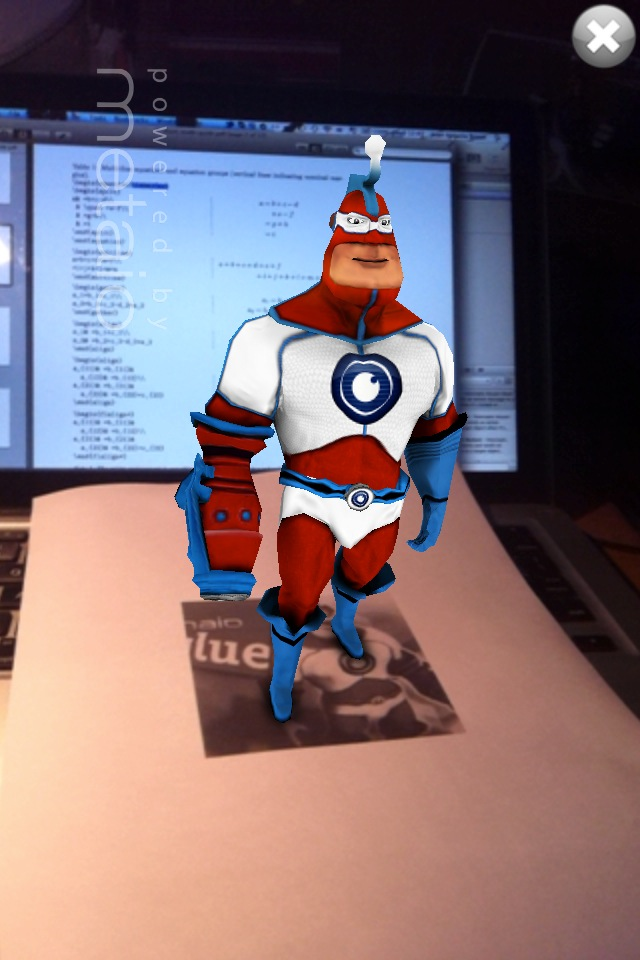
\includegraphics[scale=0.222]{figs_alcance/metaio.png} & 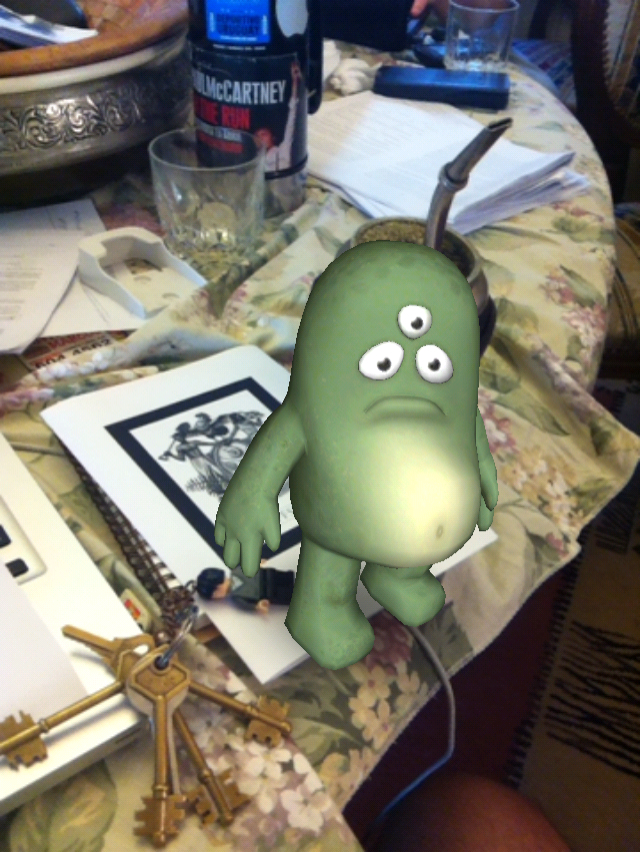
\includegraphics[scale=0.5]{figs_alcance/string.png}
\end{array}
$$
\caption{Izq.: Ejemplo de realidad aumentada que incluye por defecto el kit de desarrollo \textit{Metaio}. Der.: Otro ejemplo de realidad aumentada inclu�do por \textit{String}.}
\label{fig: metaioystring}
\end{figure}

Si bien se probaron algunas de estas herramientas y se tomaron de ellas est\'andares en cuanto a la \textit{performance} que una aplicaci\'on de realidad aumentada debe tener, \textbf{no es un objetivo} del proyecto el desarrollo de aplicaciones de realidad aumentada con kits de desarrollo ya existentes. Se hace hincapi\'e en la investigaci\'on de herramientas y adquisici\'on de experiencia propia, con el objetivo de marcar una hoja de ruta para todo aquel que desee continuar la investigaci\'on con nuevas ideas y algoritmos. Se deja a disposici\'on de cualquier interesado el c\'odigo de la aplicaci\'on final, los algoritmos implementados o editados, as\'i como toda la documentaci\'on.

\section{Explicaci�n global de la aplicaci�n}
\label{sec: app}
Si bien se dijo que la creaci�n de la aplicaci�n integral, correspondiente a un recorrido en realidad aumentada para muesos, corresponde tan s�lo a un quinto del alcance total del proyecto; la visualizaci�n de la aplicaci�n total es quiz� la forma m�s sencilla de comprender el proyecto en su conjunto.\\

Esta se desglosa en tres grandes bloques:

\begin{itemize}
\item \textbf{Navegaci�n}
\item \textbf{Identificaci�n de obras}
\item \textbf{Realidad aumentada}
\end{itemize}
que son resumidos individualmente en secciones subsiguientes.


\subsection{Navegaci�n}
La navegaci�n es la ubicaci�n del usuario dentro del museo, �til tanto para el usuario como para la aplicaci�n, ya que sabiendo en qu� regi�n del museo este se encuentra, se simplifica un poco la identificaci�n de la obra. Se estudiaron distintas alternativas para la navegaci�n. La primera posibilidad analizada fue la utilizaci�n de tres o m�s \textit{access points}, mediante los cuales, una vez mapeadas las caracter�sticas de las se\~nales en cada uno de los puntos de las salas, se puede ubicar al usuario dentro de las mismas. Otra forma de navegaci�n que se tuvo en cuenta fue la localizaci�n a trav�s de la tecnolog�a GPS. Sin embargo, se opt� por utilizar c�digos QR dada su amplia difusi�n, practicidad y facilidad de implementaci�n. Esta discusi�n t�cnica se ve m�s en detalle en el Cap�tulo \ref{chap: navident}.\\

\subsection{Identificaci�n de obras}
Por identificaci�n de obras se entiende al proceso mediante el cual la aplicaci�n detecta frente a qu� obra se encuentra el usuario para as� entonces brindarle informaci�n de la misma, una audiogu�a y si fuera el caso la posibilidad de desplegar realidad aumentada sobre ella. La forma en la que se implement� este bloque fue mediante un algoritmo de detecci�n de caracter�sticas de im�genes llamado SIFT. Este algoritmo genera descriptores que sirven como identificadores de las im�genes y se ver� en profundidad en el Cap�tulo \ref{chap: navident}.\\

\subsection{Realidad Aumentada}

El proceso mediante el cual se logra la realidad aumentada puede verse en el diagrama de bloques de la Figura \ref{fig: bloques_ra}. Resulta muy importante aclarar que cada uno de estos bloques es perfectamente intercambiable por otro de id�ntica funci�n, tan s�lo ajustando las interfaces entre ellos.\\

\begin{figure}[h!]
\centering

\includegraphics[scale=1.2]{figs_alcance/bloques_ra.eps}
\caption{Diagrama de bloques del proceso mediante el cual se logra la realidad aumentada.}
\label{fig: bloques_ra}
\end{figure}

En el diagrama de bloques de la Figura \ref{fig: bloques_ra}, primero la c�mara toma una imagen, que luego es procesada con el objetivo de detectar en esta caracter�sticas. Estas caracter�sticas pueden ser segmentos, esquinas, descriptores; que luego son utilizados por un alg�n algoritmo de estimaci�n de la pose, que busca estimar en qu� posici�n se encuentra la c�mara respecto de cierto eje de coordenadas previamente definido y hacia d�nde esta apunta. Es de inter�s para este proyecto el utilizar en particular la detecci�n de segmentos como m�todo para la extracci�n de caracter�sticas de las im�genes adquiridas. Con la informaci�n anterior, se debe poder \textit{renderizar} una escena de manera consistente con la pose de la c�mara, para as� entonces lograr la salida del sistema, que ser� una imagen con la realidad aumentada incorporada.\\

Para este proyecto se dise\~n� un marcador formado por tres grupos de cuadrados conc�ntricos, a partir del cual se extraen los segmentos necesarios para la estimaci�n de la pose del dispositivo. El bloque de detecci�n de caracter�sticas est� compuesto por los bloques del diagrama de la Figura \ref{fig: bloques_correspondencias}.\\
\begin{figure}[h!]
\centering

\includegraphics[scale=1.2]{figs_alcance/bloques_correspondencias.eps}
\caption{Diagrama de bloques de la detecci�n de caracter�sticas utilizada en este proyecto.}
\label{fig: bloques_correspondencias}
\end{figure}

En el diagrama de bloques de la Figura \ref{fig: bloques_correspondencias}, primero se detectan idealmente todos los segmentos que hay en la imagen y luego mediante cierto algoritmo se filtran tan s�lo los pertenecientes al marcador antedicho y se agrupan por cuadrado. En el tercer bloque, se hallan las esquinas de estos cuadrados mediante la intersecci�n de los segmentos. Finalmente, mediante cierta l�gica, estos puntos son ordenados de una manera predefinida. Detalles respecto de este proceso y sobre el marcador utilizado se ven en el Cap�tulo \ref{ch:marcadores}.\\

\section{Sobre el documento}

En el presente documento se ver�n en detalle todos los aspectos t�cnicos referidos a los temas vistos en este cap�tulo. Se explica claramente la investigaci�n realizada, los algoritmos utilizados, las herramientas aprendidas y en general, toda la experiencia adquirida a lo largo del proyecto. Se justifican claramente todas las decisiones que hubo que tomar y se comentar� adem�s, en cada caso, si estas fueron acertadas o no.\\

En el Cap�tulo \ref{chap: hwysw} se comparan ambas plataformas y se justifica la elecci�n de una de ellas. Luego se ven m�s a fondo algunas caracter�sticas de la plataforma seleccionada y finalmente algunas herramientas gen�ricas requeridas para el desarrollo. En el Cap�tulo \ref{chap: navident} se ven en detalle las soluciones t�cnicas para la navegaci�n y la detecci�n de la obra. Los Cap�tulos \ref{ch:detection} y \ref{ch:marcadores} abarcan respectivamente los temas detecci�n de caracter�sticas de las im�genes en general; y detalles respecto de marcadores comunmente utilizados en aplicaciones de realidad aumentada, siendo una adaptaci�n de estos, el marcador utilizado en este proyecto en parcitular. \\

M�s adelante, en el Cap�tulo \ref{chap: lsd}, se estudia a fondo un algoritmo de detecci�n de segmentos en im�genes digitales llamado LSD, utilizado para la detecci�n de segmentos representada en el primer bloque de la Figura \ref{fig: bloques_correspondencias}. Luego, en el Cap�tulo \ref{chap: camypose}, se plantea un modelo para la c�mara utilizada para la captura y se introducen conceptos b�sicos para comprender c�mo es el proceso de la estimaci�n de la pose de la misma. El algoritmo utilizado en este proyecto para tal fin, se presenta en el Cap�tulo \ref{chap: posit}.\\

El Cap�tulo \ref{chap: kalman} presenta el filtro de \textit{Kalman} y sus ecuaciones b�sicas. En el Cap�tulo \ref{chap: render} se introduce brevemente el concepto de \textit{render} y se presenta la herramienta utilizada para realizar \textit{renders} en la plataforma escogida. Luego, en el Cap�tulo \ref{chap: casoUso}, se presentan los distintos casos de uso implementados para probar integrar todos los bloques necesarios para la realidad aumentada en peque\~nas aplicaciones individuales. M�s adelate, en el Cap�tulo \ref{chap: imp}, se explican los detalles t�cnicos respecto de la aplicaci�n completa, tal y como se define en la secci�n \ref{sec: app}.\\

Las herramientas utilizadas para analizar el desempe\~no y la validaci�n de cada algoritmo se explican en el Cap�tulo \ref{chap: benchmark}. Finalmente, en el Cap�tulo \ref{chap: costos}, se analizan los costos econ�micos que tuvo el proyecto.
\chapter{Hardware y Software}
\label{chap: hwysw}
\section{Introducci�n}
Introducci�n
\section{Software de procesamiento de im�genes}
Software de procesamiento de im�genes
\subsection{Lenguaje C}
Ventajas del Lenguaje C para procesamiento de im�genes
\subsection{Librer�as y recursos}
\subsubsection{OpenCV}
\subsubsection{IPOL}
\subsubsection{ITK e ImageMagik}

\section{Elecci�n de plataforma}
La elecci�n de la plataforma para desarrollar fue una de las primeras desiciones que se tuvo que hacer m�s all� del proceso natural inicial de investigaci�n del proyecto. Esto es debido a que existen muchos factores que se ven afectados en funci�n de la plataforma que se eligiera que van desde aprendizaje de lenguaje, entorno de desarrollo hasta la adquisici�n de plataformas y/o m�quinas para desarrollar. As� entonces las dos grandes posibilidades que se ten�an al comienzo y que determinaban estos factores era la elecci�n de trabajar en plataformas que tuvieran los sistemas operativos Android o iOS (en ning�n momento se consider� desarrollar sobre plataformas con Symbian dado que est� en proceso de desaparici�n). Uno de los aspectos desfavorables que se ve�a sobre Android era la multiplicidad de plataformas existentes, de distintas caracter�sticas de procesamiento, c�mara y sensores entre otras cosas con respecto a las plataformas que utilizan iOS. Por otra parte luego de un proceso de investigaci�n se vio que el conjunto de herramientas existentes y el estado de maduraci�n del desarrollo de aplicaciones para iOS hac�an de este sistema operativo, un camino m�s seguro para comenzar en un �rea que era desconocida. Es sabido que Android es un sistema operativo que viene en pleno crecimiento y que a nivel masivo es una buena alternativa desarrollar en �l, pero para los fines de investigaci�n y de desarrollo de sotware que ten�a el presente proyecto se vio que era mejor desarrollar sobre iOS y plataformas Apple.\\

Al trabajar con Apple entonces se cuenta con la ventaja de contar con pocas variantes en cuanto al Hardware utilizado. B�sicamente existen tres familias de dispositivos en los que se puede desarrollar: iPhone, iPad y iPod Touch. Para cada variante de plataforma existen distintos modelos que hacen que algunas caracter�sticas importantes como la capacidad de procesamiento, la resoluci�n de c�mara o el tama\~no de la pantalla entre otras puedan verse afectadas. A continuaci�n se presenta brevemente c�mo fue el surgimiento de cada uno de los dispositivos al mercado y se describen resumidamente las principales caracter�sticas.
\subsection{iPhone, iPad, iPod Touch}
\subsubsection{Comparaci�n de plataformas.}
Sin dudas el iPhone fue uno de los saltos m�s grandes en el mundo tecnol�gico en los �ltimos a\~nos. Logr� llenar el hueco que los PDAs de la d�cada de los 90 no hab�an sabido completar y comenz� a desplazar al invento que revolucion� el mercado de los contenidos de m�sica, el iPod. Gracias a su pantalla t�ctil capacitiva de alta sensibilidad logr� reunir todas las funcionalidades agregando solamente un gran bot�n y algunos extra para controlar volumen o desbloquar el dispositivo. \\
La primera generaci�n del iPhone fue lanzada por Apple en Junio de 2007 en Estados Unidos, luego de una gran inversi�n de la operadora AT\&T que exig�a exclusividad de venta dentro de dicho pa�s durante los siguientes cuatro a\~nos. La misma soportaba tecnolog�a GSM cuatribanda y se lanz� en dos variantes de 4GB y 8GB de ROM. El segundo modelo lanz� como novedad el soporte de tecnolog�a 3G cuatribanda y GPS asistido. Luego le siguieron el iPhone 3GS, 4, 4S y el 5, siendo este �ltimo, la sexta y �ltima generaci�n disponible al momento de la redacci�n de este trabajo.\\

%http://ipod.about.com/od/ipadcomparisons/a/ipad-iphone-3gs-ipod-touch.htm
%http://www.apple.com/ipod-touch/specs.html
%http://www.apple.com/iphone/specs.html
%http://www.apple.com/ipod-touch/fourth-generation-specs.html
%http://www.apple.com/ipad/compare/

%http://en.wikipedia.org/wiki/List_of_iOS_devices
%http://en.wikipedia.org/wiki/IPod_Touch
%http://en.wikipedia.org/wiki/IPhone
%http://en.wikipedia.org/wiki/IPad

%SUPPORT
%http://support.apple.com/kb/SP587
%http://support.apple.com/kb/SP643
%http://support.apple.com/kb/SP594
%http://support.apple.com/kb/SP622

%PLATFORM NOTES
%http://developer.apple.com/library/ios/#documentation/3DDrawing/Conceptual/OpenGLES_ProgrammingGuide/OpenGLESPlatforms/OpenGLESPlatforms.html

%BENCHMARK GPU
%http://www.anandtech.com/show/4216/apple-ipad-2-gpu-performance-explored-powervr-sgx543mp2-benchmarked

%COMPARE
%http://www.gsmarena.com/compare.php3

%GPU SGX
%http://developer.apple.com/library/ios/#documentation/3DDrawing/Conceptual/OpenGLES_ProgrammingGuide/OpenGLESPlatforms/OpenGLESPlatforms.html
Por su parte tanto el iPad como el iPod Touch tambi�n representaron un gran salto en el mundo de las plataformas y \textit{Tablets}, agrandando las posibilidades de desarrollo y procesamiento. Como se dijo, de cada una de estas tres familias de dispositivos existen distintas versiones y modelos. Por eso, a continuaci�n se muestra una tabla comparativa de determinadas caracter�sticas que son de inter�s a los 
efectos del presente proyecto.

\tiny
\begin{table}[htbp]
\caption{Comparativa de algunas plataformas Apple}
\begin{tabular}{|l|l|l|l|l|}
\hline
& \textbf{iPhone 4} & \textbf{iPhone 4s} & \textbf{iPod Touch 4G} & \textbf{iPad 2} \\ \hline

\textbf{ROM} & \scriptsize 8, 16 o 32 GB & \scriptsize 16, 32 o 64 GB & \scriptsize 8, 32 o 64 GB & \scriptsize  16, 32 o 64 GB \\ \hline

\textbf{RAM} & \scriptsize 512 MB  & \scriptsize 512 MB & \scriptsize 256 MB & \scriptsize 512 MB \\ \hline

\textbf{SoC} & \scriptsize Apple A4 & \scriptsize Apple A5 & \scriptsize Apple A4 & \scriptsize Apple A5 \\ \hline

\textbf{CPU} & \scriptsize 1 GHz, ARM Cortex-A8 & \scriptsize 1 GHz,  dual-core ARM Cortex-A9 & \scriptsize 800 MHz, ARM Cortex-A8 & \scriptsize 1 GHz  dual-core ARM Cortex-A9   \\ \hline

\textbf{GPU} & \scriptsize PowerVR SGX535 GPU & \scriptsize PowerVR SGX543MP2 & \scriptsize PowerVR SGX535 GPU & \scriptsize PowerVR SGX543MP2 \\ 
		    & \scriptsize  & \scriptsize  (2-core) GPU & \scriptsize  & \scriptsize  (2-core) GPU \\ \hline

\textbf{C�MARA} & \scriptsize Foto: 5.0 MP & \scriptsize Foto: 8.0 MP & \scriptsize Foto: 0.7 MP & \scriptsize Foto: 0.7 MP \\ 
				    	& \scriptsize  Video: 720p HD (30 fps) & \scriptsize  Video: 1080p HD (30 fps) & \scriptsize Video: 720p HD (30 fps) & \scriptsize Video: 720p HD (30 fps) \\ \hline

\textbf{PANTALLA} & \scriptsize Diagonal: 3.5'' & \scriptsize Diagonal: 3.5'' & \scriptsize Diagonal: 3.5'' & \scriptsize Diagonal: 9.7'' \\ 
				  & \scriptsize Pixels: 960x640 & \scriptsize Pixels: 960x640 & \scriptsize Pixels: 960x640 & \scriptsize Pixels: 1024x768 \\ 
				  & \scriptsize Densidad de Pixels: 326 ppi  & \scriptsize  Densidad de Pixels: 326 ppi  & \scriptsize Densidad de Pixels: 326 ppi  & \scriptsize  Densidad de Pixels: 123 ppi \\ 
				  & \scriptsize Multit�ctil & \scriptsize Multit�ctil & \scriptsize Multit�ctil & \scriptsize Multit�ctil \\ \hline


\textbf{SENSORES} & \scriptsize Girs�scopo de 3 ejes & \scriptsize Girs�scopo de 3 ejes & \scriptsize Girs�scopo de 3 ejes & \scriptsize Girs�scopo de 3 ejes \\
& \scriptsize Aceler�metro  & \scriptsize Aceler�metro & \scriptsize Aceler�metro & \scriptsize Aceler�metro\\
& \scriptsize Sensor de luz ambiente & \scriptsize Sensor de luz ambiente & \scriptsize  Sensor de luz ambiente & \scriptsize  Sensor de luz \\ 
& \scriptsize Sensor de proximidad & \scriptsize Sensor de proximidad &  & \\ \hline
\end{tabular}
\label{tab: compHWiOS}
\end{table}
\normalsize
%http://www.edaboard.com/thread75452.html

%Microcontroller and System-on-a-chip
%Seminar on Embedded Systems Architecture
%Peter Thoman (peter.thoman@uibk.ac.at)
%University of Innsbruck 2009-12-03
\subsubsection{Algunas caracter�sticas a detallar.}
Hay algunos comentarios respecto de la Tabla \ref{tab: compHWiOS} que es bueno destacar. Primeramente, es importante decir que se eligieron esos cuatro dispositivos pues pareci� de inter�s conocer al menos una plataforma de cada familia y dentro de las mismas se eligieron las que fueron utilizadas para desarrollar.\\
Uno de los puntos a evaluar es el \textbf{SoC}, que refiere a \textit{System on Chip} por sus siglas en ingl�s. \textit{System on Chip} es un concepto de los sistemas embebidos que refiere a la integraci�n de todo lo necesario para poder correr un sistema operativo, en un solo circuito integrado. En contraposici�n a un microcontrolador que es capaz de realizar procesamiento m�s b�sico y menos potente, con poca interacci�n de usuario y menor flexibilidad, un \textit{SoC} refiere a la idea de tener todo lo necesesario para desarrollar sobre la plataforma y poder hacer procesamiento sin tantas limitaciones. B�sicamente cumplen funciones similares pero el \textit{SoC} forma parte de una evoluci�n de los microcontroladores, siendo de una complejidad mayor e integrado en un tama\~no muy reducido buscando poco consumo y eficiencia de costos. As� entonces un \textit{SoC} puede estar conformado por un microcontrolador y hardware adicional como procesadores de se\~nal y bloques de memoria.  \\
%http://www.arm.com/products/processors/cortex-a/index.php
En la Figura \ref{fig: soc} se ilustran los dos tipos de \textit{SoC} de los dispositivos de la Tabla \ref{tab: compHWiOS}: Apple A4 y Apple A5. Algunos dispositivos que no figuran en la tabla como el \textit{iPhone 5} o el \textit{iPad 4} usan \textit{SoCs} m�s recientes como el Apple A6 o Apple A6x respectivamente. La familia de \textit{SoCs} Apple Ax, es la que la mencionada firma utiliza en todas sus plataformas, inclusive en el \textit{Apple TV} y es manufacturada por Samsung. Estos \textit{SoCs} se caracterizan por utilizar CPUs de arquitectura ARM, en su mayor�a ARMv7 y GPUs de PowerVR de la l�nea SGX. \\

\begin{figure}[h!]
\centering
$
\begin{array}{cc}
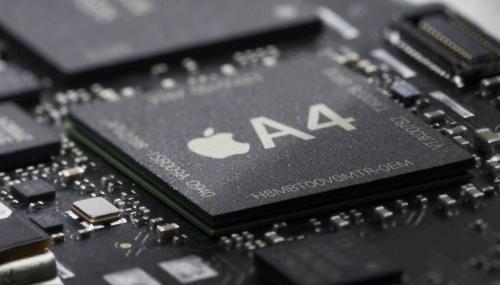
\includegraphics[scale=0.3]{figs_hwysw/applea4.png} & 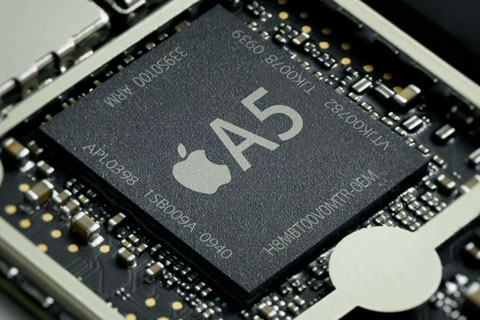
\includegraphics[scale=0.3]{figs_hwysw/applea5.png} \\
\end{array}
$
\caption{\textit{System on Chip}: SoC.}
\label{fig: soc}
\end{figure}

La arquitectura ARM incorpora algunas caracter�sticas de la arquitectura RISC (\textit{Reduced Instruction Set Computer}) como el hecho que las operaciones sean llevadas a cabo sobre un conjunto de registros a tales efectos y no sobre la memoria directamente. Otra caracter�stica que tiene de RISC es que tiene un modo simple de direccionamiento donde las direcciones son tambi�n guardadas sobre registros destinados a tales efectos. La mayor�a de los procesadores est�n hechos con un ancho de palabra de 32-bit salvo el reciente ARMv8 que incorpora la posibilidad de utilizar ambos anchos de palabra: 32-bit o 64-bit. Otra caracter�stica a destacar sobre estos procesadores es que es posible programar sobre ellos utilizando lenguaje C/C++. Por m�s informaci�n sobre esta arquitectura referirse a la web de la empresa \url{http://www.arm.com}.\\
Por su parte las GPU utilizadas en los \textit{SoCs} de la serie Apple Ax, son GPUs de PowerVR, una divisi�n de la firma Imagination Technologies (\url{http://www.imgtec.com/}) que desarrolla hardware y software para \textit{rendering} 2D y 3D, procesamiento de im�genes y codificaci�n. La funci�n que tiene la GPU es asignar a cada pixel de la pantalla su color para cada cuadro. En particular, estas GPU implementan un concepto innovador de \textit{renderizado} que mejora notoriamente la performance de los gr�ficos: \textit{Tile-Bassed Deferred Rendering} (TBDR). Este concepto aprovecha la independencia de �reas alejadas de la pantalla y de la correlaci�n de p�xeles cercanos y divide la pantalla en \textit{tiles} o baldozas. A cada \textit{tile} se le asocia un procesamiento paralelo y con esto se mejora notablemente la performance respecto al m�todo tradicional: Immediate mode renderers (IMRs), que procesa la pantalla completa. Las im�genes \textit{renderizadas} est�n hechas por tri�ngulos (pol�gonos), por lo que uno de los indicadores fundamentales para evaluar la performance de una GPU es la cantidad de tri�ngulos (pol�gonos) que es capaz de procesar por segundo. En (referencia benchmark: http://www.anandtech.com/show/4216/apple-ipad-2-gpu-performance-explored-powervr-sgx543mp2-benchmarked) se puede ver un an�lsis interesante que compara entre otros, a los dos tipos de GPU que se presentaron en la Tabla \ref{tab: compHWiOS}: SGX535 y SGX543MP2. En dicho an�lisis se muestra por ejemplo que en el mejor de los casos la GPU SGX535 fue capaz de procesar 8.69 millones de tri�ngulos por segundo frente a los 29 millones procesados por la GPU SGX543MP2.\\
%http://www.imgtec.com/powervr/powervr-graphics-technology.asp


\section{Software de Apple Inc.}

\subsection{Sistemas Operativos}
Para poder desarrollar aplicaciones sobre dispositivos m�viles de la firma Apple Inc. es necesario contar con computadoras que corran el sistema operativo \textbf{Mac OS X}. Esto puede ser llevado a cabo, ya sea adquiriendo plataformas de desarrollo de la mencionada firma o creando m�quinas virtuales que corran dicho sistema operativo. Para la segunda opci�n (la m�s econ�mica pero con ciertas dificultades de performance), es necesario que la computadora cuente con virtualizaci�n de hardware. Se comenz� trabajando de esta manera hasta el momento de adquirir plataformas de desarrollo que contaran con Mac OS X en forma nativa.\\
Mac OS X refiere a la versi�n n�mero 10 (en n�meros romanos) de una serie de sistemas operativos que comenzaron a desarrollarse en la d�cada de los 80 (Mac OS 1 data del a?o 1984). En los �ltimos 28 a?os se han ido sucediendo nuevas versiones que han ido mejorando caracter�sticas en la estructura de datos con la incorporaci�n de la jerarqu�a de archivos en Mac OS 3 por ejemplo, en la b�squeda de archivos, con la simultaneidad de tareas, multiplicidad de usuarios o incluso con el �nfasis en la interfaz de usuario por mencionar algunas caracter�sticas importantes en la evoluci�n de esta familia de sistemas operativos. Dentro de Mac OS X existen distintas versiones, siendo la m�s actual la Versi�n 10.8: Mountain Lion lanzada durante 2012.\\
Por su parte todas las plataformas m�viles de Apple Inc corren otro dispositivo de c�digo cerrado: \textbf{iOS}. Originalmente llamado as� por ser el sistema operativo utilizado por la plataforma iPhone, este sistema operativo est� tambi�n en las plataformas iPad, iPod Touch y Apple TV en todas sus versiones. La versi�n m�s reciente de este SO es el iOS 6.1.\\
Una de las grandes innovaciones de estas plataformas es el hecho de poder desarrollar aplicaciones y correrlas en el propio dispositivo (por supuesto tambi�n sucede lo mismo en el mundo Android). Para poder lograr esto, es necesario como se ha dicho, contar con una m�quina que corra Mac OS X y contar con el SDK apropiado llamado \textbf{Xcode}. Este entorno de desarrollo y su lenguaje se explican en la secci�n \ref{sec: objc}.

\subsection{Objective-C}
\label{sec: objc}
%http://developer.apple.com/library/mac/#documentation/Cocoa/Conceptual/ObjectiveC/Introduction/introObjectiveC.html
El lenguaje que fue elegido por Apple Inc para desarrollar sobre plataformas m�viles es Objective-C. Este lenguaje fue desarrollado en la d�cada de 1980 como un superconjunto de C orientado a objetos. Es decir que es una extensi�n del standard ANSI C que incorpora un modelo orientado a objetos basado en \textbf{Smalltalk}. Una de las diferencias sustanciales del modelo orientado a objetos de Objective-C respecto a otros lenguajes como Java o C++, es el hecho de la invocaci�n de los m�todos (procedimientos) de las instancias de clases. En objective-C esta invocaci�n se da enviando mensajes, algo que se hereda de Smalltalk. As� entonces para invocar un m�todo se procede con el siguiente c�digo por ejemplo:
\begin{verbatim}
[receiver message];
\end{verbatim}
Donde $receiver$ es un objeto que recibe un mensaje (acci�n) $message$ a realizar. Esta acci�n puede tener par�metros asociados, como por ejemplo el siguiente c�digo real:
\begin{verbatim}
[myRectangle setWidth:20.0];
\end{verbatim}
Esta diferencia conceptual de utilizar mensajes se representa en el hecho de que en tiempo de compilaci�n estos mensajes no son m�s que una etiqueta y no est�n asociados al bloque de c�digo como es el caso de Java o C++. Entonces es factible que suceda el hecho de que ese mensaje o m�todo no est� implementado por esa clase y reci�n en tiempo de ejecuci�n es que saltar� el error al sustituirse esa etiqueta por un c�digo inexistente, pues un objeto recibe un mensaje para realizar un m�todo que no est� dentro de su repertorio. Para esto es que en la documentaci�n de Apple Inc se recomienda utilizar ciertos trucos para garantizar que el objeto que reciba el mensaje sea capaz de responder correctamente, como por ejemplo consultando primero si es capaz de realizar dicha acci�n y luego en caso de poder realizar dicha acci�n.\\
Otro detalle a destacar es que este lenguaje, al igual que Java tambi�n soporta la herencia m�ltiple. Esto es, dado un conjunto de m�todos que son comunes a un conjunto de clases pero que no llegan a tener un lazo tan fuerte como para estar jer�rquicamente relacionadas con una superclase com�n, se puede generar una clase abstracta cuyos m�todos sean implementados por m�s de una clase sin necesidad de generar ese v�nculo fuerte que es la herencia. As� como en Java existen las interfaces, que hacen esto posible, en Objective-C existen los protocolos. Existen protocolos formales e informales y con m�todos obligatorios de implementar y otros opcionales. Una clase que implemente un protocolo dado tiene que tener dentro de su encabezado declarado el nombre del protocolo. Esto es:
\begin{verbatim}
@interface ClassName : ItsSuperclass < protocol list >
\end{verbatim}
Hay otras particularidades del lenguaje pero que no van m�s all� de la sintaxis como los m�todos de clase y los m�todos de instancia, como los m�todos \textit{get} y \textit{set} para acceder y setear atributos (propiedades) de los objetos, como la notaci�n de \textit{import} en lugar de \textit{include} para quienes est�n acostumbrados a C y as� varias detalles m�s. Sin embargo m�s all� de estas y otras diferencias y particularidades resulta un lenguaje relativamente �gil y dentro de todo sencillo de aprender para quien tiene ya un conocimiento de otros lenguajes orientados a objetos. 
\subsection{Xcode: Herramientas y Librer�as}
Como se dijo anteriormente el entorno de desarrollo de aplicaciones t�pico es Xcode, el cual es gratuito y permite compilar c�digo C, C++, Objective-C, Objective-C++, Java y AppleScript. Xcode integra en una sola interfaz todo lo que involucra c�digo, dise?o de interfaz de usuario (\textbf{Interface Builder}) y \textit{debugging}. Tambi�n viene con un conjunto herramientas �tiles para evaluar la performance de la aplicaci�n en distintos aspectos que se llama \textbf{Instruments}. Por otra parte viene con un conjunto importante de \textit{Frameworks} entre los cuales se encuentran \textbf{Cocoa} y \textbf{Cocoa Touch} que proveen de herramientas �tiles para desarrollar m�s f�cilmente aplicaciones para Mac OS X e iOS respectivamente. \\
%http://developer.apple.com/library/ios/#documentation/Miscellaneous/Conceptual/iPhoneOSTechOverview/Introduction/Introduction.html#//apple_ref/doc/uid/TP40007898-CH1-SW1
%http://developer.apple.com/library/ios/navigation/#section=Frameworks&topic=EventKitUI
Las aplicaciones que corren sobre los distintos dispositivos como iPhone, iPod Touch, iPad o AppleTV est�n desarrolladas en Objective-C pero sobre la base de estas librer�as o \textit{Frameworks} de iOS que se pueden separar en cuatro grandes capas seg�n el nivel de abstracci�n: Cocoa Touch, Media, Core Services y Core OS.
\begin{figure}[h!]
\centering
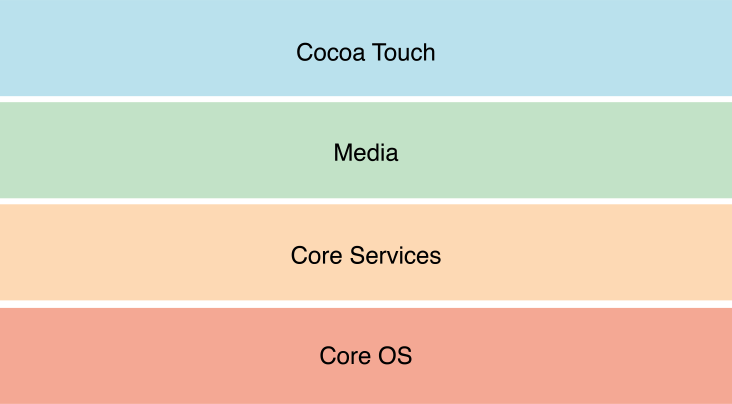
\includegraphics[scale=0.3]{figs_hwysw/iOSLayers.png}
\caption{Capas de iOS}
\label{fig: capas}
\end{figure}
%http://developer.apple.com/library/ios/#DOCUMENTATION/AudioVideo/Conceptual/AVFoundationPG/Articles/00_Introduction.html#//apple_ref/doc/uid/TP40010188
As� entonces, dentro de cada capa existen distintos \textit{Frameworks} seg�n la funcionalidad. A continuaci�n se explica un poco m�s en detalle el rol de cada capa, los distintos \textit{Frameworks} que tiene cada una y para qu� sirven.
\subsubsection{Cocoa Touch Layer}
Cocoa Touch es la capa de m�s alto nivel de iOS y es la encargada de proveer al desarrollador de ciertos \textit{Frameworks} que permitan lograr distintas tecnolog�as como la posibilidad de multitarea, el ingreso de �rdenes a la aplicaci�n a trav�s de la pantalla t�ctil, notificaciones y alertas, preservaci�n del estado de la aplicaci�n al salir de la misma, reconocimiento de gestos en la pantalla y otro tipo de funcionalidades de alto nivel. Permiten al desarrollador, sin tener que involucrarse demasiado a bajo nivel, el acceso a determinados servicios que ya est�n resueltos en forma bastante modular.\\
Cocoa Touch est� basado en la arquitectura \textbf{Modelo-Vista-Controlador}, en el que se separa en tres �reas distintas el modelo de la informaci�n, la interfaz de usuario y el conjunto de reglas que negocian la presentaci�n de la informaci�n en base a la interacci�n con el usuario. As� pues, el usuario y una aplicaci�n se podr�an considerar dos sistemas que interaccionan. Por su parte el usuario tiene como entrada la vista de la aplicaci�n y como salida tiene su respuesta a esta entrada, generando efectos sobre el control de la aplicaci�n. Por otro lado la aplicaci�n tiene como entrada las �rdenes dadas por el usuario que tienen efectos sobre el modelo de la informaci�n y este sobre la vista, quien resulta ser la salida de la aplicaci�n. Esta interacci�n se puede ilustrar con la figura \ref{fig: mvc}.
\begin{figure}[h!]
\centering
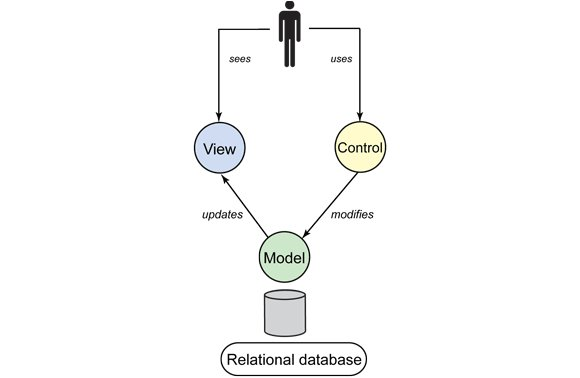
\includegraphics[scale=0.6]{figs_hwysw/mvc3.png}
\caption{Interacci�n entre las tres partes del MVC}
\label{fig: mvc}
\end{figure}
%http://developer.apple.com/library/mac/#documentation/Cocoa/Conceptual/ObjectiveC/Introduction/introObjectiveC.html 
Como se dijo, dentro de Cocoa Touch, existen distintos \textit{Framewokrs} enfocados en permitirle al desarrollador resolver en alto nivel distintos aspectos. Los mismos son los siguientes:
\begin{itemize}
\item[(1)] Address Book UI Framework
\item[(2)] Event Kit UI Framework
\item[(3)] Game Kit Framework
\item[(4)] iAd Framework
\item[(5)] Map Kit Framework
\item[(6)] Message UI Framework
\item[(7)] Twitter Framework
\item[(8)] UIKit Framework
\end{itemize}
Quiz� sea bueno mencionar que varias de estas API no fueron utilizadas en el presente proyecto dada su funci�n espec�fica y que no fueron necesarias. Sin embargo hay una en particular que tiene bastante importancia y que permite la mayor�a de las funcionalidades b�sicas que toda aplicaci�n tiene. Se trata del \textbf{UIKit}, encargado de gestionar la aplicaci�n, su interfaz de usuario y gr�ficos, encargado soportar eventos frente al toque de la pantalla, de manejar sensores como el aceler�metro y giroscopio, y de tener acceso a la c�mara y galer�a de fotos entre lo m�s importante a destacar. El soporte de la multitarea y de \textbf{Storyboards} tambi�n est� a cargo de este \textit{Framework}.\\
Hay funcionalidades que han ido cambiando con las distintas versiones de iOS. Una de ellas y quiz� una que ha generado bastantes diferencias respecto a versiones anteriores a iOS 5, es esta �ltima, el Storyboard, una herramienta muy �til de programaci�n gr�fica, que permite generar instancias de clases y v�nculos entre las mismas en forma visual a la vez de ser una contraparte de interfaz de usuario. Con una biblioteca de objetos disponibles, listos para ser usados, mediante el uso de Storyboard se hace accesible con algunas horas de dedicaci�n implementar aplicaciones sencillas. Esta herramienta vino para sustituir los archivos \textit{.nib} que permit�an dise?ar la interfaz pero no tantas funcionalidades program�ticas como el Storyboard. En particular �ste �ltimo permite agregar la funcionalidad de \textit{segues}, encargados de vincular un \textit{ViewController} con otro. Este tipo de diferencias vinieron con la idea de evitar la necesidad de implementar ciertos bloques de c�digo en forma repetitiva. Un Storyboard luce como en la figura \ref{fig: story}.
\begin{figure}[h!]
\centering
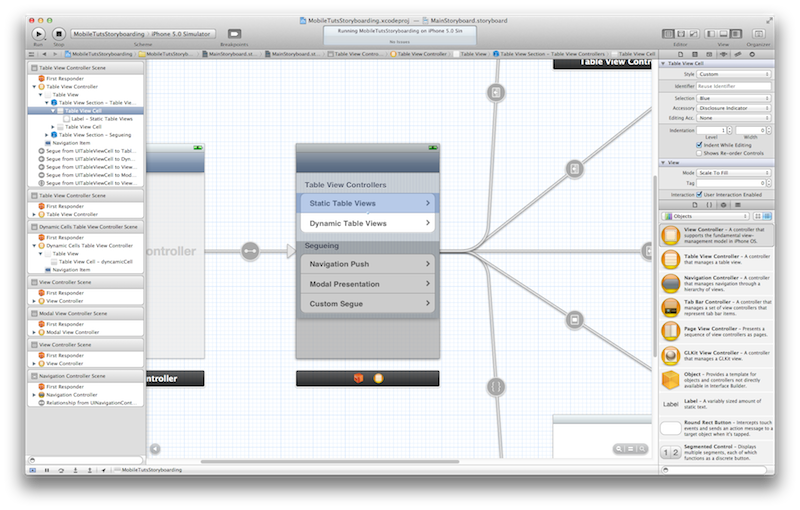
\includegraphics[scale=0.3]{figs_hwysw/story.png}
\caption{Ejemplo de Storyboard.}
\label{fig: story}
\end{figure}

Si bien se podr�a extender bastante m�s la explicaci�n sobre los detalles de Cocoa Touch, a los efectos del presente proyecto, no es de tanta relevancia excederse en este punto. 
\subsubsection{Media Layer}
\textit{Media Layer} es la capa encargada de gestionar correctamente elementos multimedia y es posible ditinguir tres grandes grupos que engloban distintos \textit{Frameworks}: Gr�ficos, Audio y Video. \\
Dentro de las tecnolog�as m�s destacadas est� todo lo vinculado a \textbf{gr�ficos} 2D y 3D, dentro de lo que se puede incluir algunos \textit{Frameworks} bastante utilizados en el presente proyecto, tales como: \textbf{Core Graphics}, muy utilizado para dibujos 2D, \textbf{Quartz Core}, quien contiene las herramientas necesarias para interactuar con otro \textit{Framework} para animaci�n de vistas, de una capa de m�s bajo nivel como \textit{Core Animation}, que es comentado m�s adelante en la secci�n \ref{sec: coreserv}. Tambi�n es parte de lo vinculado a gr�ficos, el \textit{Framework} \textbf{Core Image}, conteniendo lo vinculado a procesamiento de im�genes a trav�s filtros que utilizan directamente la lu unidad de procesamiento de gr�ficos (GPU) y otros dos \textit{Frameworks} bastante importantes en lo que respecta a \textit{rendering} como \textbf{Open GL ES} y \textbf{GLKit} (utilizado por el motor de juegos \textit{Isgl3d} entre otros).\\
Por otra parte hay otra gran familia de \textit{Frameworks} dentro de Media Layer que apunta a resolver todo lo vinculado al manejo de audio, ya sea de grabaci�n como procesamiento y reproducci�n de alta calidad. Existen algunos SDK como \textbf{iSpeech} o \textbf{Dragon Mobile} que resuelven de manera similar al proyecto Siri, el procesamiento de la voz humana reconociendo palabras e interpretando, que utilizan algunos de los \textit{Frameworks} de procesamiento de audio de esta familia. \\
En cuanto a lo vinculado al manejo de video, como parte de esta capa, se tienen dos \textit{Framework} importantes con distintos niveles de abstracci�n: \textbf{MediaPlayer} y \textbf{AVFoundation}. Tambi�n existen otros \textit{Frameworks} fuera de esta capa que son capaces de manejar video como la clase UIImagePickerController (muy utilizada en el proyecto) del mencionado UIKit. En la figura \ref{fig: avfound} se esquematiza el nivel de abstracci�n de los \textit{Frameworks} de las distintas capas que son capaces de manejar multimedia.
\begin{figure}[h!]
\centering
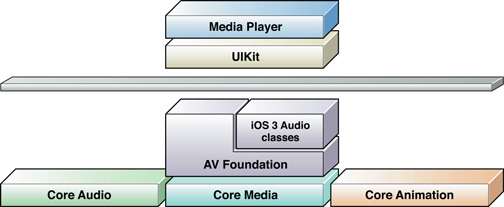
\includegraphics[scale=0.6]{figs_hwysw/avFoundation.png}
\caption{Frameworks de las distintas capas para manejo de video}
\label{fig: avfound}
\end{figure}
Con MediaPlayer es posible reproducir audio y video muy f�cilmente en determinada �rea de la pantalla ya sea desde un URL o de un archivo, es posible mostrar o no los elementos de control del video as� como tambi�n controlar, volumen y tama?o de la pantalla. Por su parte, con AVFoundation es posible capturar con la c�mara, reproducir, editar y procesar audio y video. Es posible implementar ciertos protocolos que hace de esto algo relativamente sencillo. 


\subsubsection{Core Services}
\label{sec: coreserv}
Core Services es la capa de m�s bajo nivel de iOS y contiene los elementos fundamentales sobre los que se construyen las capas superiores. Es posible que al comenzar a programar para iOS no se tenga mucha interacci�n con esta capa pero sin embargo existen algunos conceptos importantes de esta capa que s� vale la pena mencionar dado que en el presente proyecto se tuvieron que entender y discutir. Una de ellas es la \textit{Automatic Reference Counting} o \textbf{ARC}. Esta funcionalidad compete a la reserva y liberaci�n de memoria por parte de los objetos. La idea b�sica es lograr que el uso de memoria sea el m�nimo posible, logrando que los objetos existan en la medida que son necesarios y que su memoria sea liberada ni bien sea posible. 
\begin{figure}[h!]
\centering
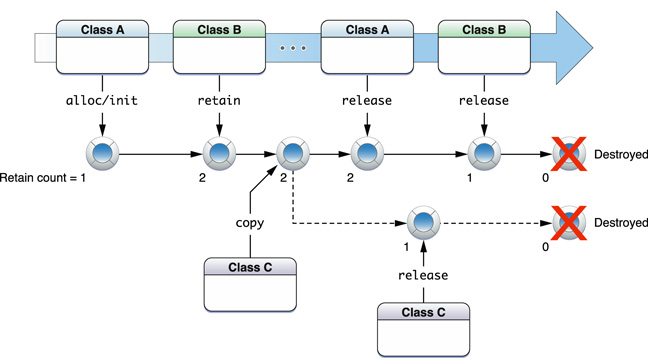
\includegraphics[scale=0.6]{figs_hwysw/mrr.png}
\caption{Ciclo de vida de objetos, Manual-Retain-Release.}
\label{fig: manualRR}
\end{figure}
T�picamente, al crear una instancia de un objeto se incrementa un contador y al liberar se decrementa y entonces se tiene cierto control sobre la reserva y liberaci�n de memoria en base al contador. Sin embargo, la liberaci�n de memoria reservada por objetos queda bajo la responsabilidad del desarrollador y en casos de un c�digo complejo puede llegar a ser habitual olvidarse de la liberaci�n de memoria.	 Lo anterior refiere a una gesti�n manual de la reserva y liberaci�n conocido como \textit{manual retain-release}. Para no tener que enfrentar este tema y poder instanciar clases sin tener presente la posterior liberaci�n de memoria (pues quiz� se sepa cu�ndo no ser� m�s necesario un objeto o no), se utiliza ARC. Esta funcionalidad eval�a el ciclo de vida de los objetos y agrega c�digo en tiempo de compilaci�n en caso de considerarlo necesario. Es bueno aclarar que esto refiere a memoria reservada pura y exclusivamente por objetos, es decir mediante \textit{alloc}. En caso de tratarse de memoria reservada para variables de lenguaje C (\textit{malloc}), es necesario proceder de igual manera que en dicho lenguaje, liberando la memoria mediante un \textit{free}. \\
Adem�s del ARC, Core Services permite el manejo de archivos XML y manejo de base de datos SQL as� como tambi�n la protecci�n de datos cuando el dispositivo est� bloqueado entre otros servicios importantes. Tiene varios \textit{Frameworks} como \textbf{Core Media} que logran un nivel a�n m�s bajo que AVFoundation para el manejo de multimedia, \textbf{Quick Look} para las vistas previas de archivos, \textbf{Social} que viene a suplantar el \textit{Framework} para la utilizaci�n de Twitter que existe en iOS 5 y extiende la gesti�n para otras redes sociales, \textbf{Core Motion} para el manejo de sensores como el aceler�metro y el giroscopio, \textbf{Core Telephony} para el manejo de la informaci�n de red del dispositivo como elemento de la red de telefon�a, \textbf{CFNetwork} para el manejo de protocolos de red como http, https, ftp y resoluci�n de servidores DNS, entre otros \textit{Frameworks} importantes dentro de la capa.
%manual reference counting http://developer.apple.com/library/ios/#documentation/Cocoa/Conceptual/MemoryMgmt/Articles/MemoryMgmt.html#//apple_ref/doc/uid/10000011i
% ARC http://developer.apple.com/library/ios/#releasenotes/ObjectiveC/RN-TransitioningToARC/Introduction/Introduction.html#//apple_ref/doc/uid/TP40011226
\subsubsection{Core OS}
Con esta capa de iOS en general es dif�cil que el desarrollador tenga que involucrarse directamente dado que es la de m�s bajo nivel. Salvo que se est� frente a una aplicaci�n que requiera aspectos de seguridad o comunicaci�n con HW externo, esta capa solamente existe para ser la base sobre la cual se desarrollan los \textit{Frameworks} de las capas de m�s alto nivel. Los distintos \textit{Frameworks} que tiene est�n enfocados en resolver temas de procesamiento basados en el hardware de iOS, en comunicarse con dispositivos externos basados en iOS y de garantizar la seguridad de los datos de una aplicaci�n.


\subsubsection{Simulador}
Uno de los detalles m�s importantes del entorno de desarrollo es la capacidad de simular lo que se programa antes de probarlo en un dispositivo. Esto es �til por cuestiones de seguridad e incluso permite programar sin la necesidad de contar con una plataforma. Esto existe para \textit{Xcode} y es necesario decir que funciona muy bien, generando una representaci�n bastante fiel de lo que sucede en el dispositivo real. La �nica cr�tica que se le podr�a hacer es el hecho de no contar con c�mara y para el caso de aplicaciones de realidad aumentada esto es algo bastante importante. Sin embargo, sin ser eso, el simulador cuenta con conexi�n a internet, pantalla multit�ctil, con informaci�n de GPS ingresada por el programador, acceso a la galer�a de fotos, capacidad de procesamiento y todas las funcionalidades que un dispositivo real tiene. 
\subsubsection{Instruments}
%https://developer.apple.com/library/ios/#documentation/DeveloperTools/Conceptual/InstrumentsUserGuide/Introduction/Introduction.html#//apple_ref/doc/uid/TP40004652
Dentro de las herramientas que vienen con el entorno de desarrollo viene \textit{Instruments}, un conjunto de herramientas que permiten analizar la performance de una aplicaci�n para iOS o para Mac OS X desde distintos puntos de vista. Resulta muy �til pues muchas veces sucede que una aplicaci�n compila y se ejecuta correctamente y sin embargo puede que el desarrollador no est� conforme en cuanto a los tiempos de procesamiento o el uso de memoria consumido.\\
Para poder hacer uso del \textit{Instruments}, es necesario correr la aplicaci�n en modo \textit{Profile}. Eso despliega una ventana como la de la Figura \ref{fig: instru}. All� es posible elegir dentro de cada una de las posibilidades que ofrece \textit{Instruments}, si se quiere analizar tiempos, memoria, recursos de CPU, \textit{multithreading} entre otros tipos de datos de inter�s que es posible recoger de la aplicaci�n. Tambi�n es posible elegir la plataforma, ya sea iOS, simulador iOS o Mac OS X.\\

\begin{figure}[h!]
\centering
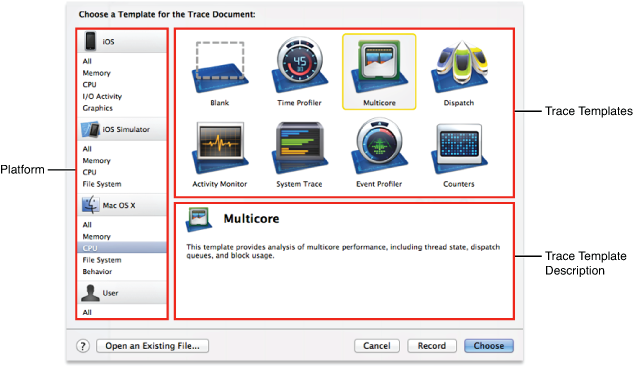
\includegraphics[scale=0.6]{figs_hwysw/instrumentsWindow.png}
\caption{Distintas opciones de \textit{Instruments}.}
\label{fig: instru}
\end{figure}
Luego de elegir el tipo de datos a ser recolectados seg�n lo que se busque analizar, se despliega una ventana como se ve en la Figura \ref{fig: instru2}. All� es necesario registrar durante varios segundos los datos mientras se corre la aplicaci�n y luego de terminado el registro, \textit{Instruments} dedica un tiempo a analizar los datos recolectados. En el detalle inferior, se desglozan los procesos que corre la aplicaci�n en forma de �rbol. Cuando se desea medir tiempos por ejemplo, esto resulta muy �til porque entre otras cosas se puede analizar qu� porcentaje del tiempo de la aplicaci�n es consumido por un m�todo en particular. Esto es posible simplemente buscando dentro del �rbol mencionado, al m�todo y leyendo el valor asignado de tiempo. Para el caso de an�lisis de memoria tambi�n es posible identificar f�cilmente en qu� parte del c�digo se est� dando alg�n problema de reserva de memoria no liberada.
\begin{figure}[h!]
\centering
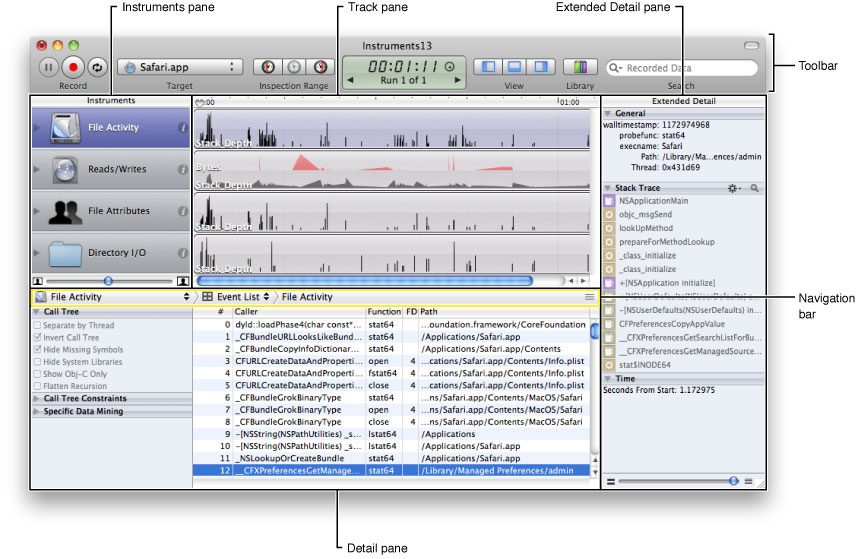
\includegraphics[scale=0.6]{figs_hwysw/instruments_tracing.png}
\caption{Trazado y an�lisis de datos recogidos.}
\label{fig: instru2}
\end{figure}
En el presente proyecto se hizo uso principalmente del \textbf{Time Profiler} que permite analizar tiempos y del \textbf{Memory Leak} que permite hacer un an�lisis de la reserva de memoria no liberada. Con los mismos fue posible optimizar tiempos en determinados m�todos del procesamiento, as� como tambi�n eliminar problemas de memoria no liberada que desencadenaban en la interrupci�n abrupta de la aplicaci�n luego de llegado un cierto nivel de reserva. Esta interrupci�n abrupta es una forma de proteger la memoria del dispositivo y evitar que se vea afectada cierta memoria �til a otros efectos. El resto de las herramientas de \textit{Instruments} fueron probadas pero no utilizadas en detalle para resolver problemas particulares.

\section{Herramientas}
Herramientas
\subsection{GIT}
\subsection{GoogleCode}
\subsection{Github}


\chapter{Detecci�n}
\label{ch:detection}

\section{Introducci�n}
En este cap�tulo se trata con algunas de las herramientas y algoritmos de detecci�n de caracter�sticas del tipo de primitivas geom�tricas como ser puntos, esquinas, bordes, l�neas, segmentos de l�nea y arcos. 

El objetivo principal es mostrar qu� caracter�sticas se pueden detectar y determinar qu� algoritmos son adecuados para su posterior utilizaci�n para la estimaci�n de pose, tema que se desarrolla en los Cap�tulos \ref{chap: camypose} y en forma m�s espec�fica en el Cap�tulo \ref{chap: posit}. El tipo de caracter�sticas elegidas para su detecci�n en la aplicaci�n final est�n fuertemente ligadas con el desempe�o del algoritmo que realiza dicha detecci�n. Existe un requerimiento de tiempo ya que la aplicaci�n final se debe ejecutar en tiempo real. Tambi�n se desea que la caracter�stica seleccionada ofrezca la posibilidad de ser procesada posteriormente mediante algoritmos relativamente simples.

Se busca que las caracter�sticas detectadas, asociadas a objetos o elementos presentes en la escena, presenten estabilidad en su ubicaci�n frente a cambios en la pose. En forma m�s espec�fica, si se tiene una esquina a detectar en una escena, por ejemplo de una mesa, la esquina puede ser detectada en im�genes o ``fotos'' de la mesa desde distintas posiciones y que en todos los casos la esquina detectada corresponde con la esquina de la mesa en la foto. Tambi�n se busca que las caracter�sticas sean robustas frente a cambios en las condiciones en que se adquiere la imagen. Estas condiciones podr�an ser iluminaci�n, presencia de ruido, oclusiones, etc.

El cap�tulo comienza con la revisi�n de algunos detectores cl�sicos de bordes y esquinas como son Canny y Harris. Posteriormente se desarrollan algunos detectores de l�neas, segmentos de l�nea y algunas estructuras m�s complejas, como el M�todo de la Transformada de Hough, LSD, EDLines y ORT. A lo largo de todo el cap�tulo se presentan resultados de estos algoritmos.
% \section{T�pos de caracter�sticas}

\section{Bordes y esquinas}
Los detectores de bordes, en particular los detectores de bordes tipo escal�n son una parte esencial de muchos sistemas de visi�n. El proceso de detecci�n de bordes cumple la funci�n de simplificar dr�sticamente la cantidad de informaci�n a procesar conservando aspectos estructurales utilizables para establecer los l�mites de cierto objeto en la imagen \cite{Canny:1986:ACA}. 

Un \textbf{borde} se puede definir intuitivamente como un cambio brusco sobre una zona en la intensidad de una imagen. M�s formalmente puede ser asociado a la b�squeda de discontinuidades y naturalmente su implementaci�n est� relacionada con la derivada primera de una imagen. En una imagen una derivada primera puede ser aproximada de distintas formas por un operador de gradiente como lo son los operadores de Sobel, Prewitt o Roberts por ejemplo\cite{operador_gradiente}. Hay implementaciones de detecci�n de bordes que toman en cuenta el \textit{efecto rampa} y por lo tanto acuden a derivadas de segundo y tercer orden. El efecto rampa se muestra en la Figura \ref{fig:rampa} en donde se puede ver en lo que aparentemente ocurre una discontinuidad en la imagen si uno se acerca lo suficiente a la regi�n, esta discontinuidad es en realidad continua.
\begin{figure}[h!]
  \centering
    
\includegraphics[scale=0.8]{figs_detection/rampa.png}
  \caption{Efecto rampa. A la izquierda una imagen que presenta una discontinuidad. A la derecha una acercamiento en la regi�n marcada en rojo.}
  \label{fig:rampa}
\end{figure}
	
\subsection{Detector de bordes de Canny}
El detector de bordes de Canny fue desarrollado en 1986 por John F. Canny \cite{Canny:1986:ACA} en el art�culo \emph{``A Computational Approach to Edge Detection''} con el objetivo de descubrir el algoritmo de detecci�n de bordes �ptimo. En esta secci�n se describe brevemente el algoritmo y se muestran algunos resultados de inter�s. La presentaci�n de este algoritmo est� inspirada principalmente en el art�culo del detector de bordes de Canny de Wikipedia \cite{canny_wiki}.\\ %\footnote{\url{http://en.wikipedia.org/wiki/Canny_edge_detector}}.

Las caracter�sticas buscadas por Canny para el detector de borde �ptimo son:
\begin{itemize}
 \item \textbf{Buena detecci�n}: El algoritmo debe marcar todos los bordes reales en la imagen como sea posible.
 \item \textbf{Buena localizaci�n}: Los bordes marcados deben estar lo m�s cercanos posibles a los bordes reales en la imagen.
 \item \textbf{Respuesta m�nima}: Dado un borde en la imagen este no debe ser marcado m�s de una vez y de ser posible la presencia de ruido no debe crear falsos bordes.
\end{itemize}
En la Figura \ref{fig:resultado_canny_lena}(b) se muestra un ejemplo del detector de bordes de Canny para la imagen de Lena original \ref{fig:resultado_canny_lena}(a).

\begin{figure}[h!]
  \centering
  \subfigure[Imagen de entrada: Lena]{
    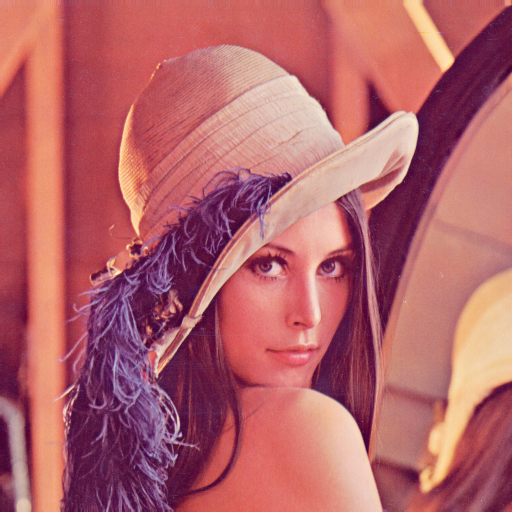
\includegraphics[scale=0.35]{figs_detection/canny/input_0.png}}
  \subfigure[Imagen de salida: Canny]{
    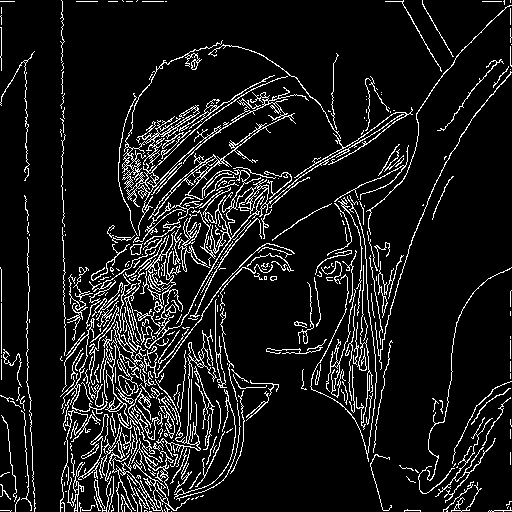
\includegraphics[scale=0.35]{figs_detection/canny/output.png}}
  \caption{Detector de bordes de Canny para la imagen Lena con par�metros: $\sigma=1.6$, $th_{lo}=4.0$, $th_{hi}=20.0$}
  \label{fig:resultado_canny_lena}
\end{figure}

El algoritmo consiste en cuatro etapas b�sicas las cuales se describen a continuaci�n. A lo largo de estas etapas se ejemplifica mediante el uso del demo \emph{online} de Canny en IPOL \cite{ipol_canny} para la imagen de Lena. Estos resultados intermedios se encuentran en la Figura \ref{fig:resultado_canny_lena_inter}.
\begin{itemize}

 \item 
\textbf{Reducci�n de Ruido}: Debido a que el detector de bordes de Canny es sensible a la presencia de ruido en las im�genes se utiliza en una primera etapa un filtrado Gaussiano en donde se realiza la convoluci�n de la imagen con un n�cleo Gaussiano. El resultado da lugar a una imagen levemente borrosa como se puede observar en la Figura \ref{fig:resultado_canny_lena_inter}(a).

 \item 
\textbf{Gradiente de intensidad de la imagen}: De forma de detectar bordes en todas las direcciones posibles, respecto a vecinos inmediatos de un p�xel, se utilizan cuatro filtros para detectar bordes en direcciones horizontal, vertical, y las dos direcciones diagonales. Un operador de detecci�n de bordes, por ejemplo Roberts, Prewitt o Sobel, devuelve un valor para la derivada primera en la direcci�n horizontal ($\mathbf{G}_x$) y otro para la derivada primera en la direcci�n vertical ($\mathbf{G}_y$). En base a estos valores se puede obtener m�dulo y direcci�n del gradiente sobre cada p�xel (Figura \ref{fig:resultado_canny_lena_inter}(b)). 
\begin{eqnarray}
\mathbf{G} = \sqrt{\mathbf{G}_x^2 + \mathbf{G}_y^2} \\
\Theta = \arctan\left(\frac{\mathbf{G}_y}{\mathbf{G}_x}\right)
\end{eqnarray}
Finalmente el �ngulo de direcci�n del borde es redondeado a uno de los cuatro �ngulos ($0$, $45$, $90$ o $135$ grados).

 \item 
\textbf{Supresi�n de no-m�ximos}: Dados los estimadores del gradiente de la imagen se realiza una b�squeda para determinar si el m�dulo del gradiente asume un rol de m�ximo local. De esta etapa se obtiene un conjunto puntos en forma de imagen binaria llamados \emph{``thin edges''} como se puede ver en la Figura \ref{fig:resultado_canny_lena_inter}(c). Estos proporcionan informaci�n de direcci�n para realizar el umbralizado con hist�resis.  

La b�squeda de m�ximos se realiza observando el �ngulo del punto y el m�dulo de �l y sus vecinos. Por ejemplo, si el �ngulo del gradiente pertenece al conjunto de los de cero grados (el borde es vertical) se observa el m�dulo de sus vecinos horizontales. Si el m�dulo del gradiente del punto es mayor a los de estos entonces el punto asume un rol de m�ximo local. Los otros casos son an�logos.

 \item 
\textbf{Umbrales con hist�resis}: El umbralizado con hist�resis requiere de dos umbrales, uno bajo y uno alto. El umbral alto asegura que se marcan bordes de los cuales se puede estar suficientemente seguros de que son borde (Figura \ref{fig:resultado_canny_lena_inter}(d)). Luego en base a los bordes correspondientes a umbrales altos se aplica el umbral bajo recorriendo los caminos de direcci�n obtenidos previamente. Una vez finalizado el proceso se tiene una imagen binaria en donde cada p�xel es marcado como borde o no (Figura \ref{fig:resultado_canny_lena_inter}(e)).
\end{itemize}

El algoritmo consiste en una serie de par�metros que ya fueron mencionados pero que vale la pena resaltar. En primer lugar el par�metro $\sigma$, la desviaci�n estandar del filtro Gaussiano utilizado en la etapa de reducci�n de ruido. Este par�metro afecta notablemente el desempe�o del algoritmo y debe ser ajustado seg�n la aplicaci�n ya que aporta un compromiso entre el detalle para bordes m�s fino y la cantidad de falsos bordes producto del ruido. Por otro lado en la etapa de umbralizado con hist�resis se tienen dos par�metros m�s, los valores de los dos umbrales; alto y bajo. En estos dos par�metros residen los t�picos problemas de los umbrales y no hay un enfoque gen�rico que lo solucione, si el umbral alto es muy alto se puede perder informaci�n importante y por otro lado si el umbral bajo es muy bajo se producir�n m�s falsos bordes debido a ruido. 
\begin{figure}[h!]
  \centering
  \subfigure[Reducci�n de ruido: Blur]{
    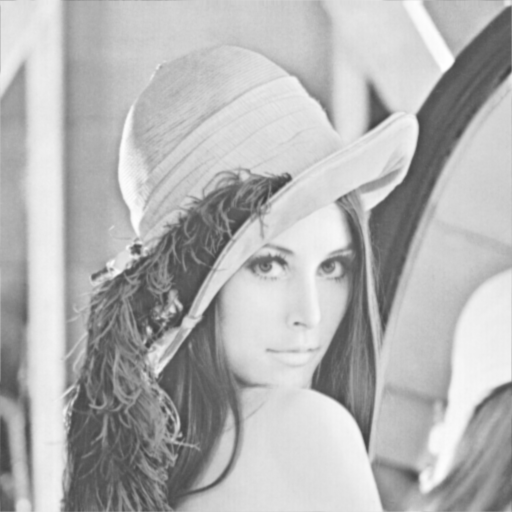
\includegraphics[scale=0.28]{figs_detection/canny/o_blur.png}}
  \subfigure[Gradiente]{
    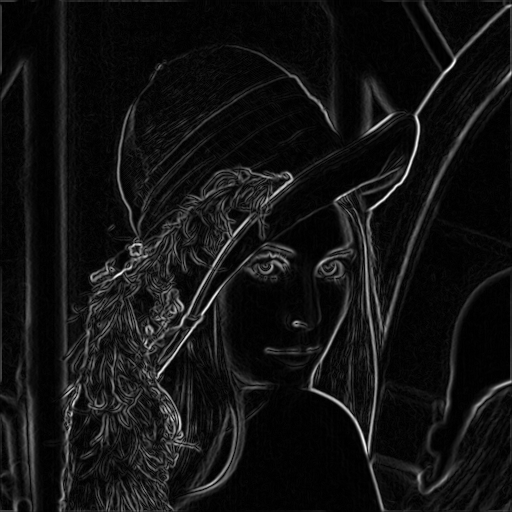
\includegraphics[scale=0.28]{figs_detection/canny/o_gradient.png}}
  \subfigure[Supresi�n de no-m�ximos]{
    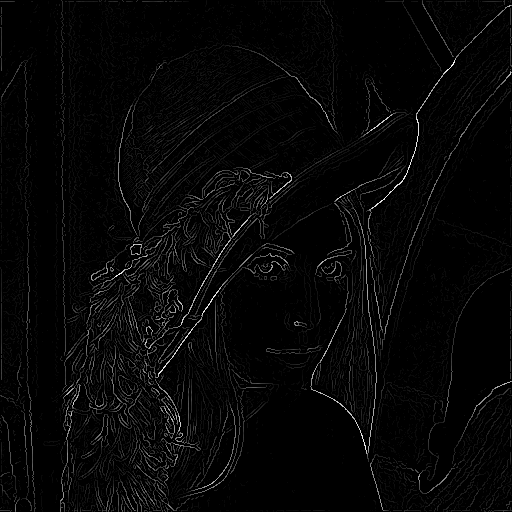
\includegraphics[scale=0.28]{figs_detection/canny/o_maxima.png}}
  \subfigure[Umbralizado con hist�resis: umbral alto]{
    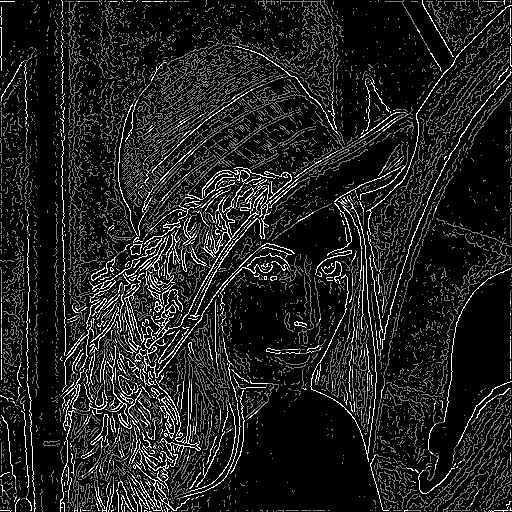
\includegraphics[scale=0.28]{figs_detection/canny/o_hi.png}}
  \subfigure[Umbralizado con hist�resis: umbral bajo]{
    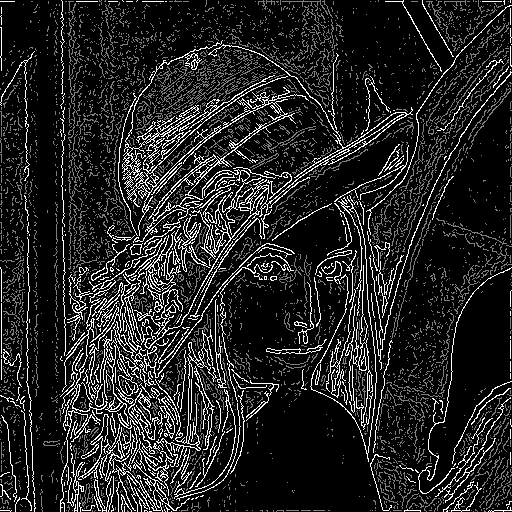
\includegraphics[scale=0.28]{figs_detection/canny/o_lo.png}}
  \caption{Resultados intermedios del detector de bordes de Canny para la imagen Lena con par�metros: $\sigma=1.6$, $th_{lo}=4.0$, $th_{hi}=20.0$}
  \label{fig:resultado_canny_lena_inter}
\end{figure}


\subsubsection{Ejemplos de inter�s}
En la Figura \ref{fig:resultado_canny_marcador} se muestran distintos resultados de Canny para distinto valor de $\sigma$, utilizando como entrada una imagen conteniendo el marcador utilizado en el proyecto.
\begin{figure}[h!]
  \centering
  \subfigure[Imagen de entrada: Marcador]{
    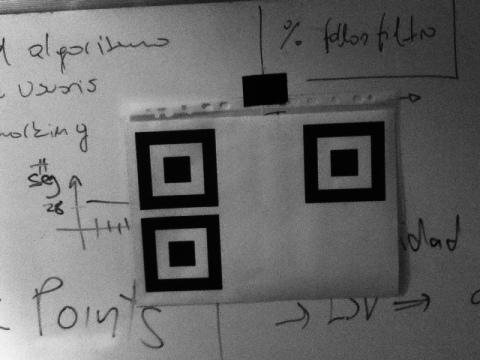
\includegraphics[scale=0.4]{figs_detection/canny_mrkr/canny_in.png}}
  \subfigure[$\sigma=0.5$]{
    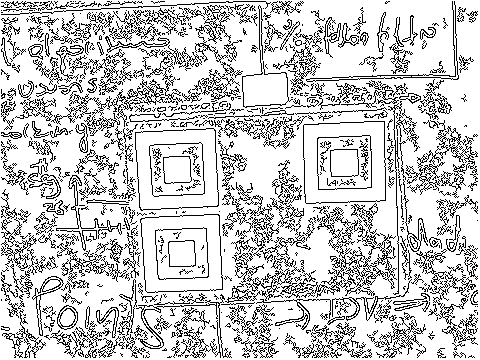
\includegraphics[scale=0.4]{figs_detection/canny_mrkr/canny_05.png}}
  \subfigure[$\sigma=1.4$]{
    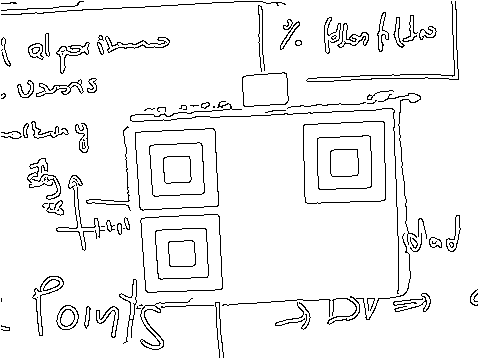
\includegraphics[scale=0.4]{figs_detection/canny_mrkr/canny_14.png}}
  \subfigure[$\sigma=6.0$]{
    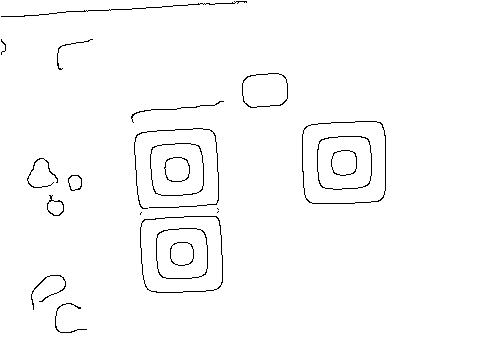
\includegraphics[scale=0.4]{figs_detection/canny_mrkr/canny_60.png}}
  \caption{Resultados del detector de bordes de Canny variando el par�metro de reducci�n de ruido $\sigma$ para una imagen de entrada conteniendo un marcador. $th_{lo}=0.2$, $th_{hi}=0.8$ (umbrales normalizados}
  \label{fig:resultado_canny_marcador}
\end{figure}
Se puede ver que con $\sigma = 0.5$ la presencia de ruido afecta notablemente la detecci�n produciendo una gran cantidad de falsos bordes. Para $\sigma=1.4$ la detecci�n es buena eliminando pr�cticamente todos los falsos bordes producto del ruido y conservando la informaci�n de borde real. Por otro lado para $\sigma=6.0$ el \emph{bluring} resulta en una detecci�n de bordes muy reducida aunque preservando la informaci�n de bordes m�s significativos como los bordes del marcador los cuales son el inter�s principal en la aplicaci�n. De todas formas se produce un efecto no deseado de ``redondeo'' de los bordes asociados al uso de un n�cleo Gaussiano circular.


\subsection{Detector de bordes y esquinas de Harris}
El detector de bordes y esquinas de Harris es un m�todo desarrollado por Chris Harris et al. en 1988 en el art�culo \emph{``A combined corner and edge detector''}\cite{Harris88acombined}. 

% Se considera una ventana en el p�xel $(x,y)$ en donde se define la suma
% cuadrada ponderada de los elementos de la ventana como
% $$E_{x,y}= \sum_{u,v} w_{u,v}[I_{x+u,y+v}-I(u,v)]^2 = \sum_{u,v} w_{u,v}[xI_x+yI_y+O(x^2,y^2)]^2 $$
% en donde $w_{u,v}$ es un n�cleo gaussiano para suavizar la respuesta y los gradientes pueden ser aproximados por
% $$I_x = I*(-1,0,1) \hspace{8mm} I_y = I*(-1,0,1)^T.$$
% Para peque�os variaciones, se puede tomar la aproximaci�n 
% $$E(x,y) = Ax^2 + 2Cxy + By^2$$
% en donde $A = I_x^2*w$, $B = I_y^2*w$ y $C = I_xI_y*w$. De forma de tomar en cuenta la variaci�n de $E$ junto con la direcci�n del cambio se reformula la
% ecuaci�n anterior como 
% $$E(x,y) =  \begin{pmatrix}
% 	      x &   y
% 	    \end{pmatrix}
% 		  \begin{pmatrix}
%                    A & C \\
% 		   C & B
%                   \end{pmatrix} \begin{pmatrix}
% 				    x\\
% 				    y
% 				\end{pmatrix} = \begin{pmatrix}
% 	      x &   y
% 	    \end{pmatrix}
% 		  M \begin{pmatrix}
% 				    x\\
% 				    y
% 				\end{pmatrix}$$
% Dado que $E$ est� fuertemente relacionado con la funci�n de autocorrelaci�n, si $\alpha$ y $\beta$ son los valores propios de la matriz $M$,
% ser�n proporcionales a la curvatura de la funci�n de autocorrelaci�n formando un descriptor invariante a rotaciones de $M$. La respuesta
% a esquinas propuesta para el detector de harris es computacionalmente m�s eficiente y no es necesario calcular valores propios de la matriz $M$. Esta dada
% por 
% $$R = det(M)-k tr^2(M)$$
% en donde $k$ es una constante de sensibilidad. Las esquinas est�n representadas por los valores de $R$ positivos mientras que los bordes corresponden a los 
% $R$ negativos y con $R$ cercano a cero tendremos zonas planas. 
Si tomamos una imagen $(I)$ en escala de grises y dos regiones solapadas de la misma que distan $(x,y)$ en las direcciones $i$ y $j$ respectivamente, definidas por una ventana $w(u,v)$; la suma ponderada del cuadrado de las diferencias entre ambas regiones ser\'a:\\
\[
E(x,y) = \sum_u{\sum_v{w(u,v) \left[ I(u+x,v+y) - I(u,v) \right]^2}}
\]
en donde $w_{u,v}$ es un n�cleo Gaussiano para suavizar la respuesta. Si realizamos una expansi\'on de Taylor de $I(u+x,v+y)$, obtenemos la siguiente aproximaci\'on:\\
\[
I(u+x,v+y) \approx I(u,v) + I_x(u,v)x + I_y(u,v)y
\]
Los gradientes de la imagen representados por $I_x$, $I_y$  pueden ser aproximados por:
$$I_x = I*(-1,0,1) \hspace{8mm} I_y = I*(-1,0,1)^T.$$
Reemplazando entonces:
\[
E(x,y) \approx \sum_u{\sum_v{w(u,v) \left[  I_x(u,v)x + I_y(u,v)y \right]^2}}
\]
o lo que es lo mismo:
\[
E(x,y) = ( \: x\:,\:y\: ) 
A 
\left(\begin{array}{c}
x\\
y
\end{array}\right)
\]
siendo:
\[
A = 
\left( 
\begin{array}{cc}
\left<I_x^2\right> & \left<I_xI_y\right> \\
\left<I_xI_y\right> & \left<I_y^2\right> 
\end{array} 
\right)
\]
donde los par\'entesis angulares denotan el promediado ponderado que puede ser, como se explica anteriormente, Gaussiano.\\

Por construcci\'on, es f\'acil ver que grandes variaciones en $E(x,y)$ ocasionadas por cambios en ambas direcciones $(i,j)$ estar\'an indicando la existencia de una esquina, mientras que grandes variaciones en $E(x,y)$ ocasionadas por cambios en una sola de direcci\'on indicar\'an la existencia de un borde. Es posible entonces limitar el estudio a la matriz A y sus valores propios.\\
Sean $\alpha$ y $\beta$ los valores propios de A. Se concluye por lo anterior que si:
\begin{itemize}
\item
Ambos valores propios son grandes: Se est� en presencia de una esquina.
\item
Un valor propio es grande y el otro peque\~no: Se est� en presencia de un borde.
\item
Ambos valores propios son peque\~nos: Se est� en presencia de una regi\'on ``plana''.
\end{itemize}
En la Figura \ref{fig:Fundamento1} se muestra la clasificaci�n de la regi�n correspondiente a la matriz $A$ correspondiente a las tres zonas de arriba. 
\begin{figure}[h!]
\centering
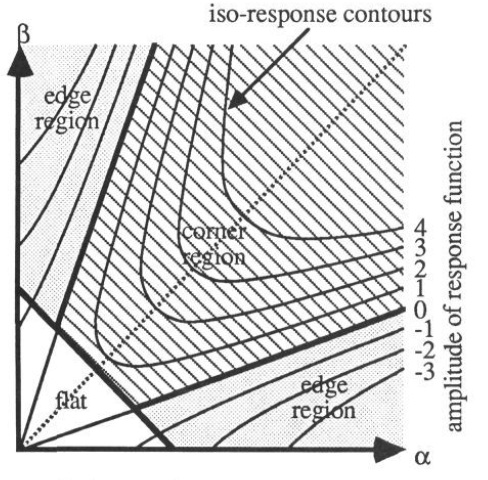
\includegraphics[scale=0.5]{figs_detection/harris/fundamento1.jpg}
\caption{Clasificaci�n de caracter�sticas seg�n los valores propios. Tomada de \cite{Harris88acombined}.}
\label{fig:Fundamento1}
\end{figure}
Debido a que el c�lculo de los valores propios de una matriz es un proceso computacionalmente costoso, se define la funci�n de respuesta $R$ que depende �nicamente de los valores propios $\alpha$ y $\beta$ y almacena b\'asicamente la misma informaci\'on.
\[
R = \alpha.\beta - k.(\alpha + \beta) = Det(A) - k.Tr(A)
\] 
donde $Det(A)$ denota el determinante de la matriz A, $Tr(A)$ su traza y $k$ es un par�metros de sensibilidad que normalmente pertenece al rango $[0.04 - 0.15]$. Por lo tanto se pueden clasificar los p�xeles de la siguiente forma:
\begin{itemize}
\item
$ R \gg 0$: Se tiene una esquina.
\item
$R \ll 0$: Se tiene un borde.
\item
$R \approx 0$: Se tiene una regi\'on ``plana''.
\end{itemize}

\subsubsection{Ejemplos de inter�s}
En la Figura \ref{fig:resultado_harris} se muestran los resultados para el detector de Harris provisto por Matlab en la funci�n \texttt{corner}. La misma tiene un par�metro modificable asociado a la m�xima cantidad de esquinas que se desean tener.
\begin{figure}[h!]
  \centering
  \subfigure[Harris para $n=50$]{
    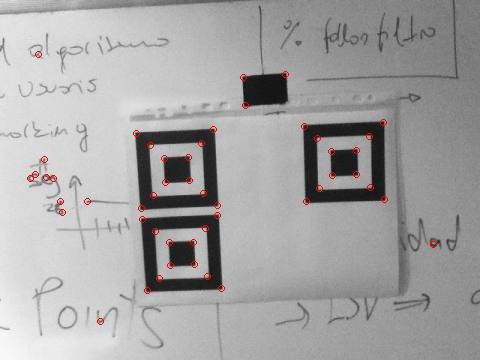
\includegraphics[scale=0.5]{figs_detection/harris/harris_50.png}}
  \subfigure[Harris para $n=100$]{
    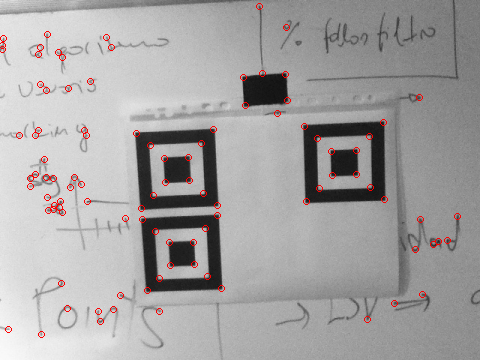
\includegraphics[scale=0.5]{figs_detection/harris/harris_100.png}}
  \caption{Resultados Harris para la imagen del marcaodor. El par�metro $n$ es un m�ximo en la cantidad de esquinas detectadas.}
  \label{fig:resultado_harris}
\end{figure}
Se puede ver que los resultados son buenos para ambos casos y particularmente buenos si se desean detectar las esquinas del marcador.

\subsubsection{Aplicabilidad}
Se pudo ver que el detector de Harris result� en una detecci�n razonable para el ejemplo tratado aunque su funcionamiento en general puede no ser tan bueno. Bajo otras condiciones menos controladas como para la detecci�n de esquinas naturales, no generadas por la presencia de un marcador, puede ser inestable y poco robusto requiriendo de alg�n tipo de validaci�n \emph{a posteriori}.

Una desventaja importante que tiene la detecci�n de caracter�sticas tipo esquinas es que si se desea saber qu� esquinas se unen entre s� mediante los lados del marcador sin ambiguedad se debe obtener m�s informaci�n que permita conectarlas. Por lo tanto un buen complemento puede ser el gradiente o una detecci�n de bordes. La detecci�n de l�neas o segmentos ya contiene esta informaci�n y por lo tanto parece m�s apropiada.

\section{L�neas y segmentos de l�nea}
Las l�neas o segmentos de l�nea son elementos que contienen una estructura m�s definida en comparaci�n con los bordes. Esta estructura definida produce a su vez que la detecci�n de este tipo de elementos sea m�s estable y menos sensible al ruido que la detecci�n de bordes o esquinas. Como se ver� en a lo largo de la secci�n, los detectores de l�neas que se presentan tienen en com�n que utilizan al inicio de la detecci�n las herramientas de gradientes y operadores gradientes o directamente la detecci�n de bordes en s� misma para realizar el objetivo de detecci�n de l�neas.

En esta secci�n de explican brevemente algunos detectores de l�neas y segmentos de l�nea. En primer lugar se menciona un detector de l�neas cl�sico y popular como es el detector de Hough y se explica su funcionamiento as� como sus principales desventajas que hacen que este m�todo sea descartado para su desarrollo en el proyecto. En segundo lugar se menciona y se hace referencia al cap�tulo en donde ser� tratado el detector de segmentos de l�nea, uno de los pilares principales de este proyecto, el LSD. Tambi�n se muestran otros detectores que fueron tomados en consideraci�n pero por diferentes razones (explicadas en su secciones correspondientes) no fueron utilizados como son el ORT y EDLines.

 \subsection{Detector de l�neas de Hough}
El M�todo de la Transformada de Hough forma parte de una t�cnica de extracci�n de caracter�sticas con fuerte aplicaci�n a detecci�n de curvas y l�neas. 

Esta t�cnica consiste en tres pasos b�sicos. En primer lugar la imagen en niveles de gris es procesada por un detector de bordes devolviendo una m�scara binaria en donde los puntos borde son marcados. En segundo lugar la Transformada de Hough es aplicada a la m�scara de forma de detectar candidatos a l�neas en forma de m�ximos locales. Esta transformada consiste en una representaci�n param�trica de formas geom�tricas. Para detecci�n de l�neas se utiliza la representaci�n
\begin{equation}
 r = xcos(\theta) + y sin(\theta)
\end{equation}
en donde $r$ representa la distancia entre la l�nea y el origen y $\theta$ es el �ngulo del vector perpendicular a la recta desde el origen. Es posible
asociar una recta al par de par�metros $(r, \theta)$. El plano $(r,\theta)$ es es plano de Hough. Se determina en este plano para cada punto de la imagen
una �nica sinusoidal en donde mediante su superposici�n se tendr�, para una serie de puntos alineados en la imagen, un punto de cruce de estas sinusoides dado
por los par�metros $(r,\theta)$. Mediante la b�squeda de m�ximos locales en el plano de Hough se tienen definidas l�neas en la imagen.

Finalmente los segmentos son extra�dos de las l�neas detectadas utilizando umbrales sobre dos par�metros geom�tricos: el largo m�nimo de un segmento y la distancia m�xima permitida entre dos segmentos consecutivos.\\

La principal desventaja del m�todo de la transformada de Hough para detecci�n de l�neas resulta ser el ajuste de par�metros. El detector de bordes contiene por lo menos un par�metro ajustable de tipo de sensibilidad, la Transformada de Hough est�ndar involucra usualmente cuatro par�metros. Uno asociado a la escala, un segundo asociado al compromiso entre falsos positivos y falsos negativos y los otros dos a la discretizaci�n de los par�metros $r$ y $\theta$, aunque estos �ltimos pueden ser asociados a la resoluci�n de la imagen. Por otro lado est�n los dos par�metros asociados a la etapa de extracci�n de segmentos \cite{GJMR08}.

El ajuste de estos par�metros puede dar problemas y desafortunadamente no hay una regla general para realizar esto. Si el ajuste es correcto este m�todo puede proveer muy buenos resultados pero en otro caso el desempe�o se puede ver fuertemente afectado.

\subsubsection{Ejemplos de inter�s}
En la Figura \ref{fig:resultado_hough} se muestran los resultados para el detector l�neas mediante el M�todo de la Transformada de Hough implementado por Matlab mediante el uso de la funci�n \texttt{houghlines}. El script utilizado se encuentra en el Centro de Documentaci�n de Mathworks\cite{matlab_hough}. Del script proporcionado se realizaron algunos cambios, se carg� la ruta de la imagen de entrada, se elimin� la rotaci�n a la imagen de entrada y se modificaron algunos par�metros. Los resultados mostrados representan los mejores casos para los distintos ajustes de par�metros probados. El tama�o m�nimo de segmento se fij� en $15$ y el m�ximo hueco entre segmentos a llenar en $8$.
\begin{figure}[h!]
  \centering
  \subfigure[El plano de Hough]{
    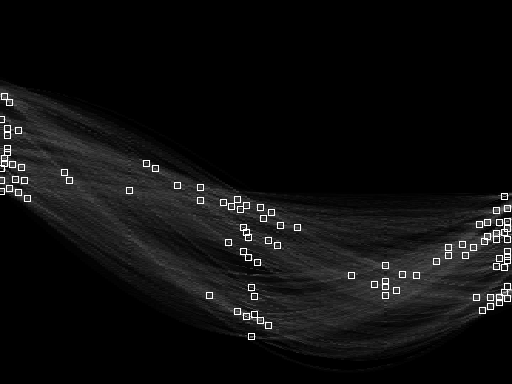
\includegraphics[scale=0.47]{figs_detection/hough/hough_transform.png}}
  \subfigure[Detecci�n de l�neas de Hough]{
    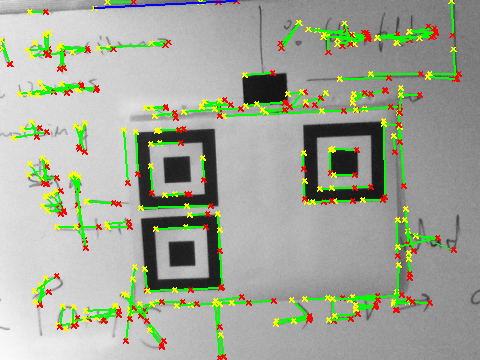
\includegraphics[scale=0.5]{figs_detection/hough/hough_lines.png}}
  \caption{Resultados para la detecci�n de l�neas por el M�todo de Hough para los par�metos: Tama�o m�nimo de segmentos $=15$, M�ximo hueco $=8$, N�mero de m�ximos $=100$ y Threshold en \texttt{houghpeaks} $=ceil(0.05*max(H(:)))$ }
  \label{fig:resultado_hough}
\end{figure}

\subsubsection{Aplicabilidad}
Se comprob� la dificultad intr�nseca del m�todo asociada al ajuste de par�metros no pudi�ndose obtener los resultados deseados en ning�n caso.

  \subsection{Detector de segmentos de l�nea: LSD}
El algoritmo Line Segment Detector (LSD) es capaz de detectar segmentos de l�nea rectos y uno de los componentes principales en este proyecto. Debido a su importancia es que se le dedica el Cap�tulo \ref{chap: lsd} a su desarrollo.

\subsubsection{Ejemplo de inter�s}
\begin{figure}[h!]
  \centering
    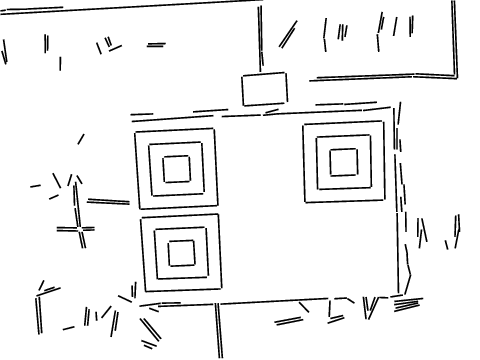
\includegraphics[scale=0.5]{figs_detection/lsd/lsd.png}
  \caption{Resultados de LSD para la imagen del marcador.}
  \label{fig:resultado_lsd_ipol}
\end{figure}
En la Figura \ref{fig:resultado_lsd_ipol} se muestran los resultados del algoritmo LSD para la imagen del marcador. Este ejemplo fue realizado mediante el uso del demo \emph{online} de IPOL para este algoritmo\cite{IpolLsd12}.

Se puede observar que el algoritmo logra detectar con �xito todas las estructuras de segmento de l�nea presentes en la imagen y en particular las que corresponden al marcador, los lados de los cuadril�teros.

El algoritmo produjo un n�mero de $169$ segmentos de l�nea detectados en un tiempo de ejecuci�n de $130ms$ sobre el servidor que aloja la aplicaci�n. La misma ejecuci�n realizada en el marco de este proyecto sobre una PC con procesador Intel Core 2 Duo de $2Ghz$ tom� un tiempo de aproximadamente $40ms$.

  \subsection{Detector de segmentos de l�nea: EDLines}
EDLines\cite{edlines} es un detector de segmentos de l�nea de tiempo lineal que provee resultados comparables con LSD. No requiere ajuste de par�metros y se ejecuta en tiempo real. En muchos aspectos es similar al LSD ya que utiliza validaci�n de l�neas mediante el principio de Helmholtz que permite controlar el n�mero de falsos positivos. El algoritmo hace uso del r�pido detector de bordes Edge Drawing (ED) \cite{edgedrawing} desarrollado por los mismos autores que provee una cadena de p�xeles borde en forma contigua.

EDLines trabaja sobre im�genes en niveles de gris y consiste b�sicamente en tres etapas: detecci�n de bordes seguido por extracci�n de segmentos y finalmente la validaci�n de l�neas. Se describen aqu� cada una de estas etapas.
\begin{itemize}
 \item 
\textbf{Detecci�n de bordes}: La detecci�n de bordes se realiza utilizando el algoritmo Edge Drawing el cual provee resultados r�pidos y libres de artefactos de ruido.

El algoritmo se aplica a la imagen de entrada en niveles de gris. En primer lugar se le aplica un filtrado para remoci�n de ruido y suavizar la imagen. A continuaci�n se calcula el gradiente, m�dulo y direcci�n, en cada pixel de la imagen suavizada. En tercer lugar se calculan un conjunto de p�xeles llamados \emph{anchors} que corresponden a puntos con alta probabilidad de ser borde. Por �ltimo se conectan estos \emph{anchors} mediante un proceso de dibujado de bordes entre ellos bas�ndose en el valor del m�dulo y direcci�n del gradiente previamente calculado. Este es en cierto sentido un proceso similar a los juegos de dibujo para ni�os.

 \item 
\textbf{Extracci�n de segmentos de l�nea}: El objetivo de esta etapa es el de ``partir'' la cadena contigua de p�xeles obtenida mediante el detector de bordes en uno o m�s segmentos de l�nea rectos. B�sicamente lo que se hace es recorrer la secuencia de p�xeles e ir ajustando l�neas a los p�xeles utilizando el m�todo de ajuste de l�neas por m�nimos cuadrados hasta que el error exceda cierto umbral. En el momento en que se excede ese umbral se genera un nuevo segmento de l�nea y as� recursivamente se recorren todos lo p�xeles de la cadena.

 \item 
\textbf{Validaci�n de l�neas}: El m�todo de validaci�n de segmentos de l�nea est� basado en el principio de Helmholtz el cual postula que para que una estructura sea perceptualmente significativa, la esperanza de que la misma (agrupado o Gestalt) ocurra de casualidad debe ser muy baja. Este es un efoque \emph{a contrario} en donde los objetos son detectados como \emph{outliers} sobre el modelo de fondo. En esta etapa se logra eliminar los falsos positivos controlando el n�mero de falsas alarmas. Este enfoque en particular es el propuesto originalmente por LSD y se explica tambi�n en el Cap�tulo \ref{chap: lsd}. 

Si la aplicaci�n lo permite, esta validaci�n puede ser eliminada o sustituida por otra, por ejemplo por un umbral de largo m�ximo de segmentos, acelerando a�n m�s el algoritmo EDLines. En LSD esta etapa esta integrada con la etapa de detecci�n de segmentos para cada iteraci�n aunque podr�a ser desacoplada en cierta medida. De todas formas EDLines presenta esa ventaja de modularidad frente a LSD que puede llegar a ser �til.
\end{itemize}

\subsection{Ejemplos de inter�s}
En la Figura \ref{fig:resultado_edlines}(a) se muestra la imagen de entrada junto con los segmentos detectados por EDLines para la imagen del marcador. En la Figura \ref{fig:resultado_edlines}(b) se muestra �nicamente los segmentos de salida de EDLines numerados.
\begin{figure}[h!]
  \centering
  \subfigure[Imagen de entrada y segmentos]{
    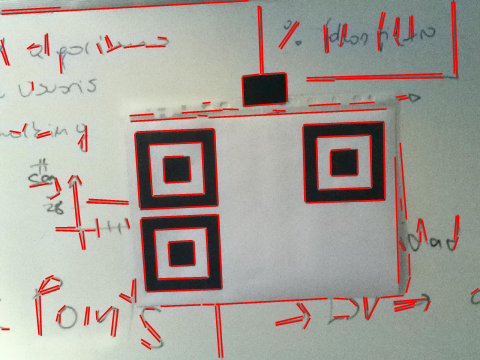
\includegraphics[scale=0.6]{figs_detection/edlines/edlines_img.png}}
  \subfigure[Segmentos de salida numerados]{
    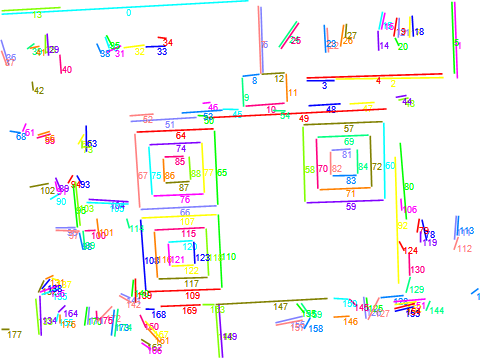
\includegraphics[scale=0.6]{figs_detection/edlines/edlines_nb.png}}
  \caption{Resultados de EDLines para la imagen del marcador.}
  \label{fig:resultado_edlines}
\end{figure}
El tiempo de ejecuci�n declarado para esta imagen por la aplicaci�n \emph{online} es de $30ms$ en su servidor pero alega que para una PC Intel con CPU de $2Ghz$ el mismo ser�a de $10ms$. Suponiendo una detecci�n en el tiempo declarado para una PC este ser�a dos veces m�s veloz que el de LSD para la misma imagen. Se detectaron $178$ segmentos y se puede ver que los resultados son muy similares a los que produce LSD que detecta $169$ segmentos para la misma imagen (Figura \ref{fig:resultado_lsd_ipol}).

\subsubsection{Aplicabilidad}
El algoritmo EDLines se encuentra disponible para descarga como una librer�a compilada para Windows o Linux. Tambi�n se puede probar en forma de demo \emph{online} desde la p�gina web del laboratorio Computer Vision \& Pattern Recognition de la Universidad de Anadolu de Turqu�a en donde tambi�n explica en forma resumida su funcionamiento\cite{edlines_demo}.\\

El c�digo fuente por su parte no est� disponible para la descarga de ning�n tipo en contraste con el LSD. Esto es un factor determinante para la utilizaci�n del algoritmo en el proyecto ya que se tiene que poder compilar para la plataforma de desarrollo utilizada, en este caso ser�a para el sistema operativo iOS. Una implementaci�n del algoritmo en lenguaje C/C++ no fue considerada como parte del alcance de este proyecto pero s� puede ser considerada como trabajo a futuro si se desea seguir con el enfoque de segmentos de l�nea para detecci�n.

  \subsection{Detector de segmentos de l�nea y arcos: ORT}
El Object Recongnition Toolkit (ORT) provee una serie de herramientas para la detecci�n de segmentos de l�nea, arcos y tambi�n puntos e incluso estructuras m�s complejas como pol�gonos. El c�digo est� disponible para su descarga en la p�gina del curso ``CSE 576 Computer Vision'' de la Univeristy of Washington de Estados Unidos de Am�rica\cite{ort_curso} como tambi�n desde un repositorio SVN p�blico se puede encontrar otra distribuci�n del c�digo con documentaci�n inclu�da\cite{ort_juanc}.

El ORT consiste en un n�mero de herramientas para ejecuci�n en cascada desde consola de comandos que resultan en la detecci�n de las caracter�sticas deseadas. Cada una de las herramientas corresponde a un algoritmo, estos son \textbf{Fex}\cite{fex}, \textbf{Lpeg}\cite{lpeg} e \textbf{Ipeg}. 

A continuaci�n de explican algunas de ellas.
\begin{itemize}

 \item 
\textbf{Chainpix}: produce una lista de p�xeles encadenados desde una imagen binaria que es salida de un detector de bordes tipo Canny. Se ejecuta mediante
\begin{verbatim}
chainpix < blocks.canny.pgm > blocks.cpx
\end{verbatim}
en donde \texttt{blocks.canny.pgm} es la imagen binaria salida de Canny y \texttt{blocks.cpx} la lista de p�xeles encadenados en un formato predefinido.

\item
\textbf{Fex}: convierte la lista de p�xeles encadenados en segmentos de l�nea rectos y arcos circulares. Su ejecuci�n se realiza mediante:
\begin{verbatim}
fex < blocks.cpx > blocks.fex
\end{verbatim}
y tiene como salida \texttt{blocks.fex}.

\item
\textbf{Lpeg}: realiza un agrupado de bajo nivel sobre los segmentos producidos por Fex hacia pares de l�neas paralelas y varios tipos de junturas. Tiene ciertos par�metros opcionales como el \emph{m�nimo largo de l�nea}, \emph{m�ximo �ngulo} tolerable entre dos l�neas paralelas y un \emph{nivel de calidad} m�nimo. Se ejecuta como:
\begin{verbatim}
lpeg < blocks.fex > blocks.lpg
\end{verbatim}
en donde la salida se escribe en \texttt{blocks.lpg}.

\item
\textbf{Ipeg}: realiza un agrupado de nivel medio sobre los conjuntos producidos por Lpeg hacia agrupaciones en tipo de ternas, esquinas y pol�gonos. Al igual que Lpeg tiene par�metros opcionales para producir �nicamente el tipo de agrupaciones de salida deseadas. Se ejecuta como:
\begin{verbatim}
ipeg < blocks.lpg > blocks.ipg
\end{verbatim}
en donde la salida se escribe en \texttt{blocks.ipg}.

\item
\textbf{Ort2Image}: toma la salida de Fex, Lpeg o Ipeg y realiza el dibujado de segmentos de l�nea rectos y segmentos de arco produciendo una imagen de salida en formato PGM.
\end{itemize}

\subsubsection{Ejemplos de inter�s}
En la Figura \ref{fig:resultado_ort} se muestran los resultados de las diferentes herramientas del ORT. Se utiliza como entrada el resultado del detector bordes de Canny para la imagen de la Figura \ref{fig:resultado_canny_marcador} para $\sigma = 1.4$ ya que fue el valor que demostr� mejores resultados entre las pruebas realizadas.
\begin{figure}[h!]
  \centering
  \subfigure[Imagen de entrada: Canny]{
    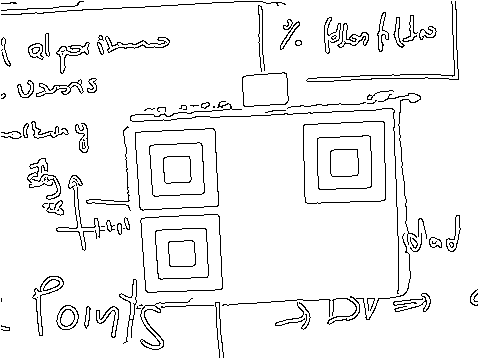
\includegraphics[scale=0.4]{figs_detection/ort/canny_140.png}}
  \subfigure[Fex]{
    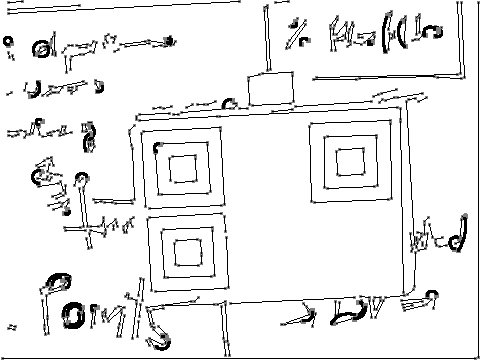
\includegraphics[scale=0.4]{figs_detection/ort/fex.png}}
  \subfigure[Lpeg]{
    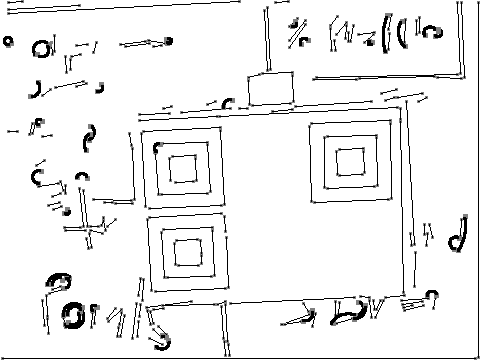
\includegraphics[scale=0.4]{figs_detection/ort/lpeg.png}}
  \subfigure[Ipeg]{
    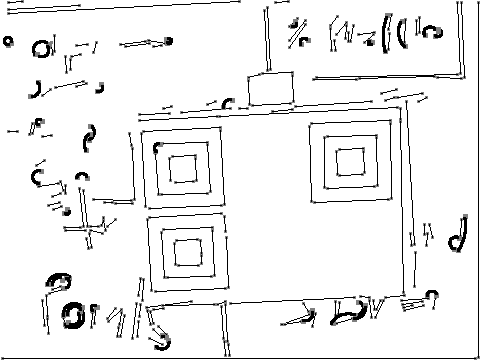
\includegraphics[scale=0.4]{figs_detection/ort/ipeg.png}}
  \caption{Resultados del Object Recognition Toolkit (ORT) para una imagen de entrada salida de Canny.}
  \label{fig:resultado_ort}
\end{figure}
Se puede observar que la salida de Fex logra capturar en buena forma los segmentos de l�nea correspondientes al marcador aunque alguno de ellos en forma ``quebrada''. Tambi�n se pueden ver los segmentos de arco detectados, otro de los elementos de este algoritmo. Lpeg logra eliminar una buena parte de los segmentos dejando s�lo aquellos que son en alg�n sentido paralelos entre s�. Por su parte Ipeg no produce ning�n cambio sobre los resultados de Lpeg. En otras pruebas realizadas tampoco se lograron los resultados deseados para este algoritmo a�n utilizando los par�metros opcionales. Un estudio m�s detallado del funcionamiento de esta herramienta en particular queda pendiente ya que resulta interesante para la aplicaci�n.

\subsubsection{Aplicabilidad}
El c�digo fuente de estas herramientas est� disponible para la descarga pero este genera un conjunto de programas ejecutables para consola de comandos. Su aplicaci�n para el proyecto no es directa ya que se deber�a portar a una interfaz compatible con nuestra aplicaci�n. Por otro lado mediante algunas pruebas realizadas sobre este algoritmo los tiempos de ejecuci�n total no resultaron suficientemente buenos para cumplir los requerimientos de tiempo real. Tambi�n se debe notar que aunque se obtuvieron resultados razonables para las herramientas Fex y Lpeg no fue as� para Ipeg que aporta un inter�s adicional para la aplicaci�n.

Un estudio m�s detallado del c�digo fuente y la posibilidad de reutilizarlo dentro del marco de la aplicaci�n queda como trabajo a futuro ya que ORT provee algunas herramientas interesantes y de m�s alto nivel que el detector de segmentos elegido LSD.

\section{Resumen}
En este cap�tulo se introdujo el tema de detecci�n de caracter�sticas orientado a primitivas. Se hizo �nfasis en el tipo de caracter�sticas de esquinas, bordes, l�neas y segmentos de l�nea recorriendo algunos algoritmos de detecci�n cl�sicos y otros m�s actuales. Se realiz� mediante el uso de un mismo ejemplo conteniendo un marcador algunas de las propiedades que interesan al proyecto concluyendo que el uso de segmentos de l�nea es el m�s apropiado por la naturaleza del marcador elegido. Se observ� que todos los algoritmos de l�neas y segmentos de l�nea analizados tienen en com�n la utilizaci�n de alg�n tipo de detecci�n de bordes o gradientes asociados a bordes al comienzo de la detecci�n. Se compararon los detectores de segmentos de l�nea obteniendo buenos resultados para los tres presentados, LSD, EDLines y ORT; eligiendo por diferentes razones LSD. A lo largo del an�lisis se establecieron pautas para realizar como trabajo a futuro en cuanto a los detectores de segmentos de l�nea, si es que se desea continuar con esta l�nea de trabajo.




\chapter{Marcadores}
\label{ch:marcadores}
\section{Introducci�n}
La inclusi�n de \emph{marcadores} en la escena ayuda al problema de extracci�n de caracter�sticas y por lo tanto al problema de estimaci�n de pose \cite{Lepetit05b}. Estos por construcci�n son elementos que presentan una detecci�n estable en la imagen para el tipo de caracter�stica que se desea extraer as� como medidas f�cilmente utilizables para la estimaci�n de la pose.

Los marcadores planos se pueden obtener mediante la construcci�n en una geometr�a coplanar de una serie de primitivas identificables como esquinas, segmentos o l�neas. Un �nico marcador plano puede contener por si solo todas las seis restricciones espaciales necesarias para definir un marco de coordenadas asociado a su pose.

Como se explica en el Cap�tulo \ref{chap: camypose} el problema de estimaci�n de pose requiere de una serie de correspondencias $\mathbf{M}_i\leftrightarrow \mathbf{m}_i$ entre puntos 3D en la escena en coordenadas del mundo y puntos en la imagen.

En el primer lugar se explican brevemente algunos de los sistemas de Realidad Aumentada m�s populares basados en marcadores planos. En segundo lugar se propone el dise�o de un marcador espec�fico para la aplicaci�n a este proyecto y se desarrollan las soluciones a los algoritmos de detecci�n de dicho marcador mostrando algunos resultados parciales en el proceso. Por �ltimo se muestran algunos resultados de Benchmark para establecer l�mites para la detecci�n.

\section{Sistemas basados en marcadores planos}
Existen muchos sistemas de visi�n basados en \emph{marcadores planos} con aplicaci�n en Realidad Aumentada y Navegaci�n. Algunos de ellos son \emph{ARToolKit}
 \cite{artoolkit}, \emph{ARTag} \cite{artag} y \emph{ARToolKitPlus} \cite{artoolkitplus} utilizados para Realidad Aumentada. A continuaci�n se realiza una breve descripci�n del funcionamiento general de los mismos.

Los sistemas basados en marcadores planos utilizan t�picamente marcadores bitonales. Esto perimte reducir la sensibilidad a las condiciones de luz de la escena y a las configuraciones de la c�mara por lo que no hay necesidad de identificar tonos de grises y la regla de decisi�n para cada p�xel puede ser reducida, en la versi�n m�s simple, a un umbral o \emph{threshold} \cite{markerdetection}. El dise�o de los marcadores depende en gran medida de la aplicaci�n. En la figura \ref{fig:Marcadores_AR} se muestran algunos marcadores planos para aplicaciones de Realidad Aumentada en donde cada uno de ellos provee suficientes puntos para permitir el c�lculo de pose tridimensional y adicionalmente contienen cierta informaci�n en su interior para permitir su identificaci�n.
\begin{figure}[h!]
  \centering
  \subfigure[\emph{ARToolKit}]{
    
\includegraphics[scale=0.45]{figs_detection/artoolkit.png}}
  \subfigure[\emph{ARTag}]{
    
\includegraphics[scale=0.45]{figs_detection/artag.png}}
  \caption{Cuatro ejemplos de marcadores para los sistemas de Realidad Aumentada indicados. Figura tomada de \cite{artag}.}
  \label{fig:Marcadores_AR}
\end{figure}

Es importante que los marcadores puedan ser localizados en un campo de visi�n amplio para permitir la correcta detecci�n bajo la distorsi�n asociada a la transformaci�n proyectiva que lleva el marcador en el mundo real al plano de imagen. Por otro lado, si los marcadores contienen informaci�n en su interior, esta no debe ser muy densa para permitir la recuperaci�n de la misma a mayor distancia. T�picamente, esta informaci�n es solo una identificaci�n entre marcadores de un mismo sistema por lo que la informaci�n es poca y esto no es un problema.

Estos sistemas contienen ciertos puntos caracter�sticos con los que se realiza el c�lculo de pose. En general su contorno es basado en un cuadril�tero y se utilizan las cuatro esquinas del contorno del marcador para realizar el c�lculo. 

Si se utiliza un �nico marcador la cantidad de puntos necesarios para la estimaci�n de pose resultan ser pocos lo que puede ser una desventaja en cuanto a la precisi�n del algoritmo de estimaci�n de pose. Esto se puede mejorar construyendo un marcador m�s complejo compuesto de una serie de marcadores y mediante la identificaci�n de los mismos asignar los puntos correspondientes para la estimaci�n de pose.

\subsection{ARToolKit}
\emph{ARToolKit} es un muy popular sistema de marcadores planos para Realidad Aumentada e Interacci�n Hombre-Computador. Su popularidad reside ser de los primeros proyectos en utilizar la Realidad Aumentada en dispositivos m�viles y tambi�n debido a que es un proyecto de c�digo abierto. 

Los marcadores bitonales consisten en un cuadrado con borde negro y un patr�n en el interior. La primer etapa del proceso de reconocimiento consisten en detectar los bordes negros. Esto se realiza buscando grupos conexos de p�xeles (\emph{blobs}) que est�n por debajo de un determinado umbral. Posteriormente se extrae el contorno de cada grupo, esos grupos que est�n rodeados por cuatro l�neas rectas son marcados como marcadores potenciales. Las cuatro esquinas de cada marcador potencial son utilizados para calcular la homograf�a y as� remover la distorsi�n perspectiva. Con el marcador en una vista can�nica, se procede a identificar el patr�n interno muestreando en una grilla, de por lo general $16\times 16$ o $32\times 32$, los valores de gris. Con esto se construye un vector caracter�stico y se compara por correlaci�n con una librer�a de vectores de caracter�sticos logrando la identificaci�n del mismo.

Este sistema tiene algunas desventajas o ``puntos d�biles''. En primer lugar la detecci�n es basada en un umbral por lo que las condiciones de iluminaci�n pueden afectar fuertemente la efectividad de la misma. Dado que el c�digo esta disponible este se puede modificar para realizar \emph{threshold} local o adaptivo por ejemplo. Otras desventajas est�n relacionadas con el proceso de identificaci�n del marcador frente a la librer�a.

\subsection{ARTag}
\emph{ARTag} es otro sistema de marcadores planos para Realidad Aumentada e Interacci�n Hombre-Computador que surge como una evoluci�n de ciertos aspectos de \emph{ARToolKit}. Los marcadores son tambi�n bitonales y basados en un borde negro. En contraste con el \emph{ARToolKit} este sistema utiliza un enfoque basado en bordes por lo que es m�s robusto a condiciones de iluminaci�n. Los bordes son unidos en segmentos que a su vez se unen en cuadril�teros. Al igual que con \emph{ARToolKit} con las esquinas se calcula la homograf�a y se muestrea en el interior del marcador pero con una grilla de $6\times 6$. 

El sistema puede lidiar con condiciones de iluminaci�n cambiantes, oclusiones y segmentos partidos hasta cierto punto. Otra mejora notable con respecto a \emph{ARToolKit} reside en el sistema de identificaci�n de marcadores. El proceso de identificaci�n de los marcadores entre s� es a su vez m�s veloz y robusto que el de \emph{ARToolKit}.

\section{Marcador QR}
El enfoque elegido para la detecci�n de caracter�sticas utilizando marcadores parte del trabajo de fin de curso denominado Autoposicionamiento 3D de \emph{Mat�as Tailani�n} y \emph{Santiago Paternain} para el curso \emph{Tratamiento de im�genes por computadora} de Facultad de Ingenier�a, Universidad de la Rep�blica\cite{tailanian}. La elecci�n se basa principalmente en los buenos resultados obtenidos para dicho trabajo con un enfoque relativamente simple. El trabajo desarrolla, entre otras cosas, un dise�o de marcador y un sistema de detecci�n de marcadores basado en el detector de segmentos LSD \cite{GJMR08} por su buena \emph{performance}. 

El marcador utilizado est� basado en la estructura de detecci�n incluida en los c�digos \emph{QR} y se muestra en la Figura \ref{fig:Marker}. �ste consiste en tres grupos id�nticos de tres cuadrados conc�ntricos superpuestos en ``capas''. La primer capa contiene el cuadrado negro de mayor tama�o, en la segunda capa se ubica el cuadrado mediano en color blanco y en la �ltima capa un cuadrado negro peque�o. De esta forma se logra un fuerte contraste en los lados de cada uno de los cuadrados facilitando la detecci�n de bordes o l�neas. El resultado de una detecci�n de l�neas para esta configuraci�n produce para cada cuadrado la detecci�n de sus lados. A diferencia de los c�digos \emph{QR} la disposici�n espacial de los grupos de cuadrados es distinta para evitar ambig�edades en la identificaci�n de los mismos entre s�. 
% Estas dos caracter�sticas son esenciales para la extracci�n de los \emph{puntos fiduciales} de forma coherente, es decir, las correspondencias tienen que poder ser determinadas completamente bajo criterios razonables.
\begin{figure}[h!]
\centering

\includegraphics[scale=0.3]{figs_detection/Marker.eps}
\caption{Marcador propuesto basado en la estructura de detecci�n de c�digos QR.}
\label{fig:Marker}
\end{figure}

\subsection{Estructura del marcador}
\label{sec:detection_estructuras}
A continuaci�n se presentan algunas definiciones de las estructuras b�sicas que componen el marcador propuesto. Estas son de utilidad para el dise�o y forman un flujo natural y escalable para el desarrollo del algoritmo de determinaci�n de correspondencias.\\

Los elementos m�s b�sicos en la estructura son los \emph{segmentos} los cuales consisten en un par de puntos en la imagen, $\mathbf{p} = (p_x,p_y)$ y $\mathbf{q} = (q_x,q_y)$. Estos \emph{segmentos} forman lo que son los lados del \emph{cuadril�tero}, el pr�ximo elemento estructural del marcador.\\

Un \emph{cuadril�tero} o \emph{quadrilateral} en ingl�s, al que se le denomina $Ql$, est� determinado por cuatro segmentos conexos y distintos entre s�. El cuadril�tero tiene dos propiedades notables; el \emph{centro} definido como el punto medio entre sus cuatro v�rtices y el \emph{per�metro} definido como la suma de el largo de sus cuatro lados. Los \emph{v�rtices} de un cuadril�tero se determinan mediante la intersecci�n, en sentido amplio, de dos segmentos contiguos. Es decir, si $s_1$ es contiguo a $s_2$ dadas las recta $r_1$ que pasa por los puntos $(\mathbf{p}_1$, $\mathbf{q}_1)$ del segmento $s_1$ y la recta $r_2$ que pasa por los puntos $(\mathbf{p}_2, \mathbf{q}_2)$ del segmento $s_2$, se determina el v�rtice correspondiente como la intersecci�n $r_1 \cap r_2$. \\
%La propiedad de conexi�n entre dos segmentos se relaja a la intersecci�n de dos discos de un cierto radio en torno a los puntos de dos segmentos vecinos. \\

A un \emph{conjunto de cuadril�teros} o \emph{quadrilateral set} se le denomina $QlSet$ y se construye a partir de $M$ cuadril�teros, con $M>1$. Los cuadril�teros comparten un mismo centro pero se diferencian en un factor de escala. A partir de dichos cuadril�teros se construye un lista ordenada $(Ql[0],Ql[1],\dots,Ql[M-1])$ en donde el orden viene dado por el valor de per�metro de cada $Ql$. Se define el \emph{centro del grupo de cuadril�teros}, $\mathbf{c}_i$, como el promedio de los centros de cada $Ql$ de la lista ordenada.\\

Finalmente el \emph{marcador QR} est� constituido por $N$ conjuntos de cuadril�teros dispuestos en una geometr�a particular. Esta geometr�a permite la determinaci�n de un sistema de coordenadas; un origen y dos ejes a utilizar. Se tiene una lista ordenada  $(QlSet[0],QlSet[1],\dots,QlSet[N-1])$ en donde el orden se puede determinar mediante la disposici�n espacial de los mismos o a partir de hip�tesis razonables.\\

Un marcador proveer� un numero de $4\times M \times N $ v�rtices y por lo tanto la misma cantidad de puntos para proveer las correspondencias $\mathbf{M}_i\leftrightarrow \mathbf{m}_i$ al algoritmo de estimaci�n de pose. De esta forma se tienen una cantidad de puntos superior a los que se podr�an tener utilizando uno de los marcadores de los sistemas como \emph{ARToolKit} a un costo de detecci�n relativamente bajo. Por otro lado se podr�a agregar alg�n patr�n para la identificaci�n de marcadores en la esquina que completa el rect�ngulo en donde no hay $QlSet$ como se realiz� en el trabajo Autoposicionamiento 3D \cite{tailanian}.

\subsection{Dise�o}
En base a las estructuras previamente definidas es que se describe el dise�o del marcador. Como ya se explic� se toma un marcador tipo QR basado en cuadril�teros y m�s espec�ficamente en tres conjuntos de tres cuadrados dispuestos en como se muestra en la figura \ref{fig:Marker}.\\

Los tres cuadril�teros correspondientes a un mismo conjunto de cuadril�teros tienen id�ntica alineaci�n e id�ntico centro. Los diferencia un factor de escala, esto es, $Ql[0]$ tiene lado $l$ mientras que $Ql[1]$ y $Ql[2]$ tienen lado $2l$ y $3l$ respectivamente. Esto se puede ver en la figura \ref{fig:QlSetDetail}. Adicionalmente se define un sistema de coordenadas con centro en el centro del $QlSet$ y ejes definidos como $\textbf{x}$ horizontal a la derecha e $\textbf{y}$ vertical hacia abajo. Esta convenci�n en las direcciones de los ejes es muy utilizada en el �rea de Procesamiento de Im�genes para definir las direcciones de los ejes de una imagen. Definido el sistema de coordenadas se puede fijar un orden a los v�rtices $v_{j_{1}}$ de cada cuadril�tero $Ql[j]$ como,
\begin{align*}
v_{j_{0}} = (a/2,a/2) && v_{j_{2}} = (-a/2,-a/2)  \\
v_{j_{1}} = (a/2,-a/2)&& v_{j_{3}} = (-a/2,a/2)
\end{align*}
con $a=(j+1)\times l$. El orden aqu� explicado se puede ver tambi�n junto con el sistema de coordenadas en la figura \ref{fig:MarkerDetail}.\\
\begin{figure}[h!]
\centering
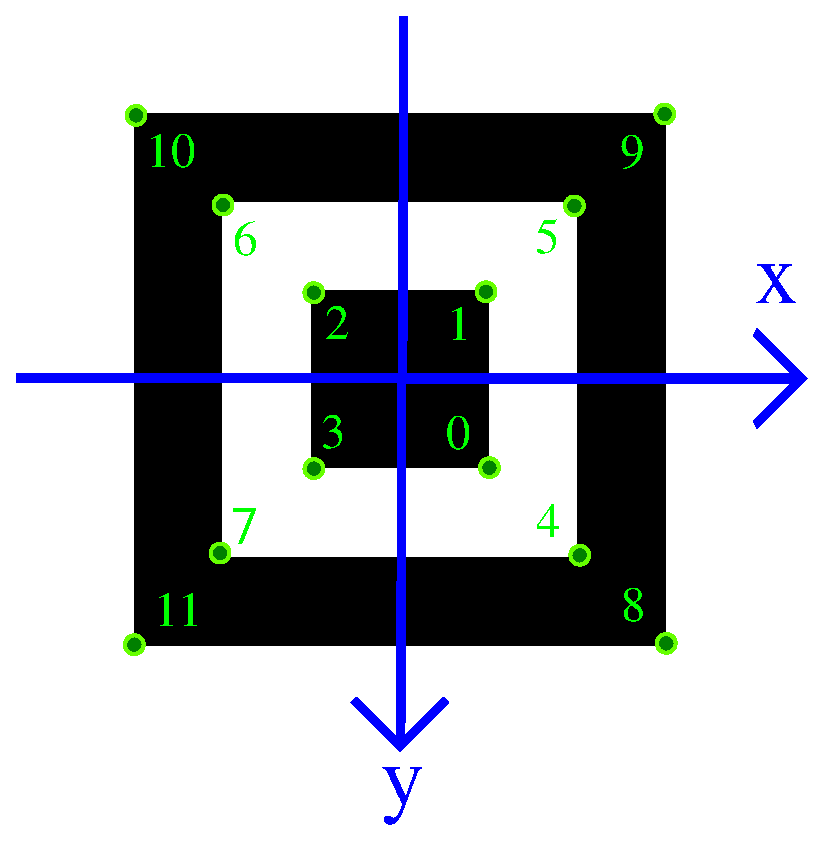
\includegraphics[scale=0.35]{figs_detection/QlSetDetail.eps}
\caption{Detalle de un $QlSet$. A la izquierda se muestra el resultado de la detecci�n de un $QlSet$ y el orden interno de sus cuadril�teros y a la derecha el orden de los v�rtices respecto al sistema de coordenadas local.}
\label{fig:QlSetDetail}
\end{figure}

Un detalle del marcador completo se muestra en la figura \ref{fig:MarkerDetail} en donde se define el conjunto $i$ de cuadril�teros conc�ntricos como el $QlSet[i]$ y se definen los respectivos centros de cada uno de ellos como $\mathbf{c}_i$. El sistema de coordenadas del marcador QR tiene centro en el centro del $QlSet[0]$ y ejes de coordenadas id�nticos al definido para cada $Ql$. Se tiene adem�s que los ejes de coordenadas pueden ser obtenidos mediante los vectores normalizados,
\begin{equation}
\begin{split}
\mathbf{x}  = \frac{\mathbf{c}_1 - \mathbf{c}_0}{||\mathbf{c}_1-\mathbf{c}_0||} & \quad
\mathbf{y}  = \frac{\mathbf{c}_2 - \mathbf{c}_0}{||\mathbf{c}_2-\mathbf{c}_0||}
\end{split} 
\label{ec:detection_ejes}
\end{equation}

La disposici�n de los $QlSet$ es tal que la distancia indicada $d_{01}$ definida como la norma del vector entre los centros $\mathbf{c}_1$ y $\mathbf{c}_0$ es significativamente mayor que la distancia $d_{02}$ definida como la norma del vector entre los centros $\mathbf{c}_2$ y $\mathbf{c}_1$. Esto es, $d_{01}\gg d_{02}$. Este criterio facilita la identificaci�n de los $QlSet$ entre s� basados �nicamente en la posici�n de sus centros y es explicado en la secci�n de determinaci�n de correspondencias (Secci�n \ref{sec:detection_correspondencias}).
\begin{figure}[h!]
\centering
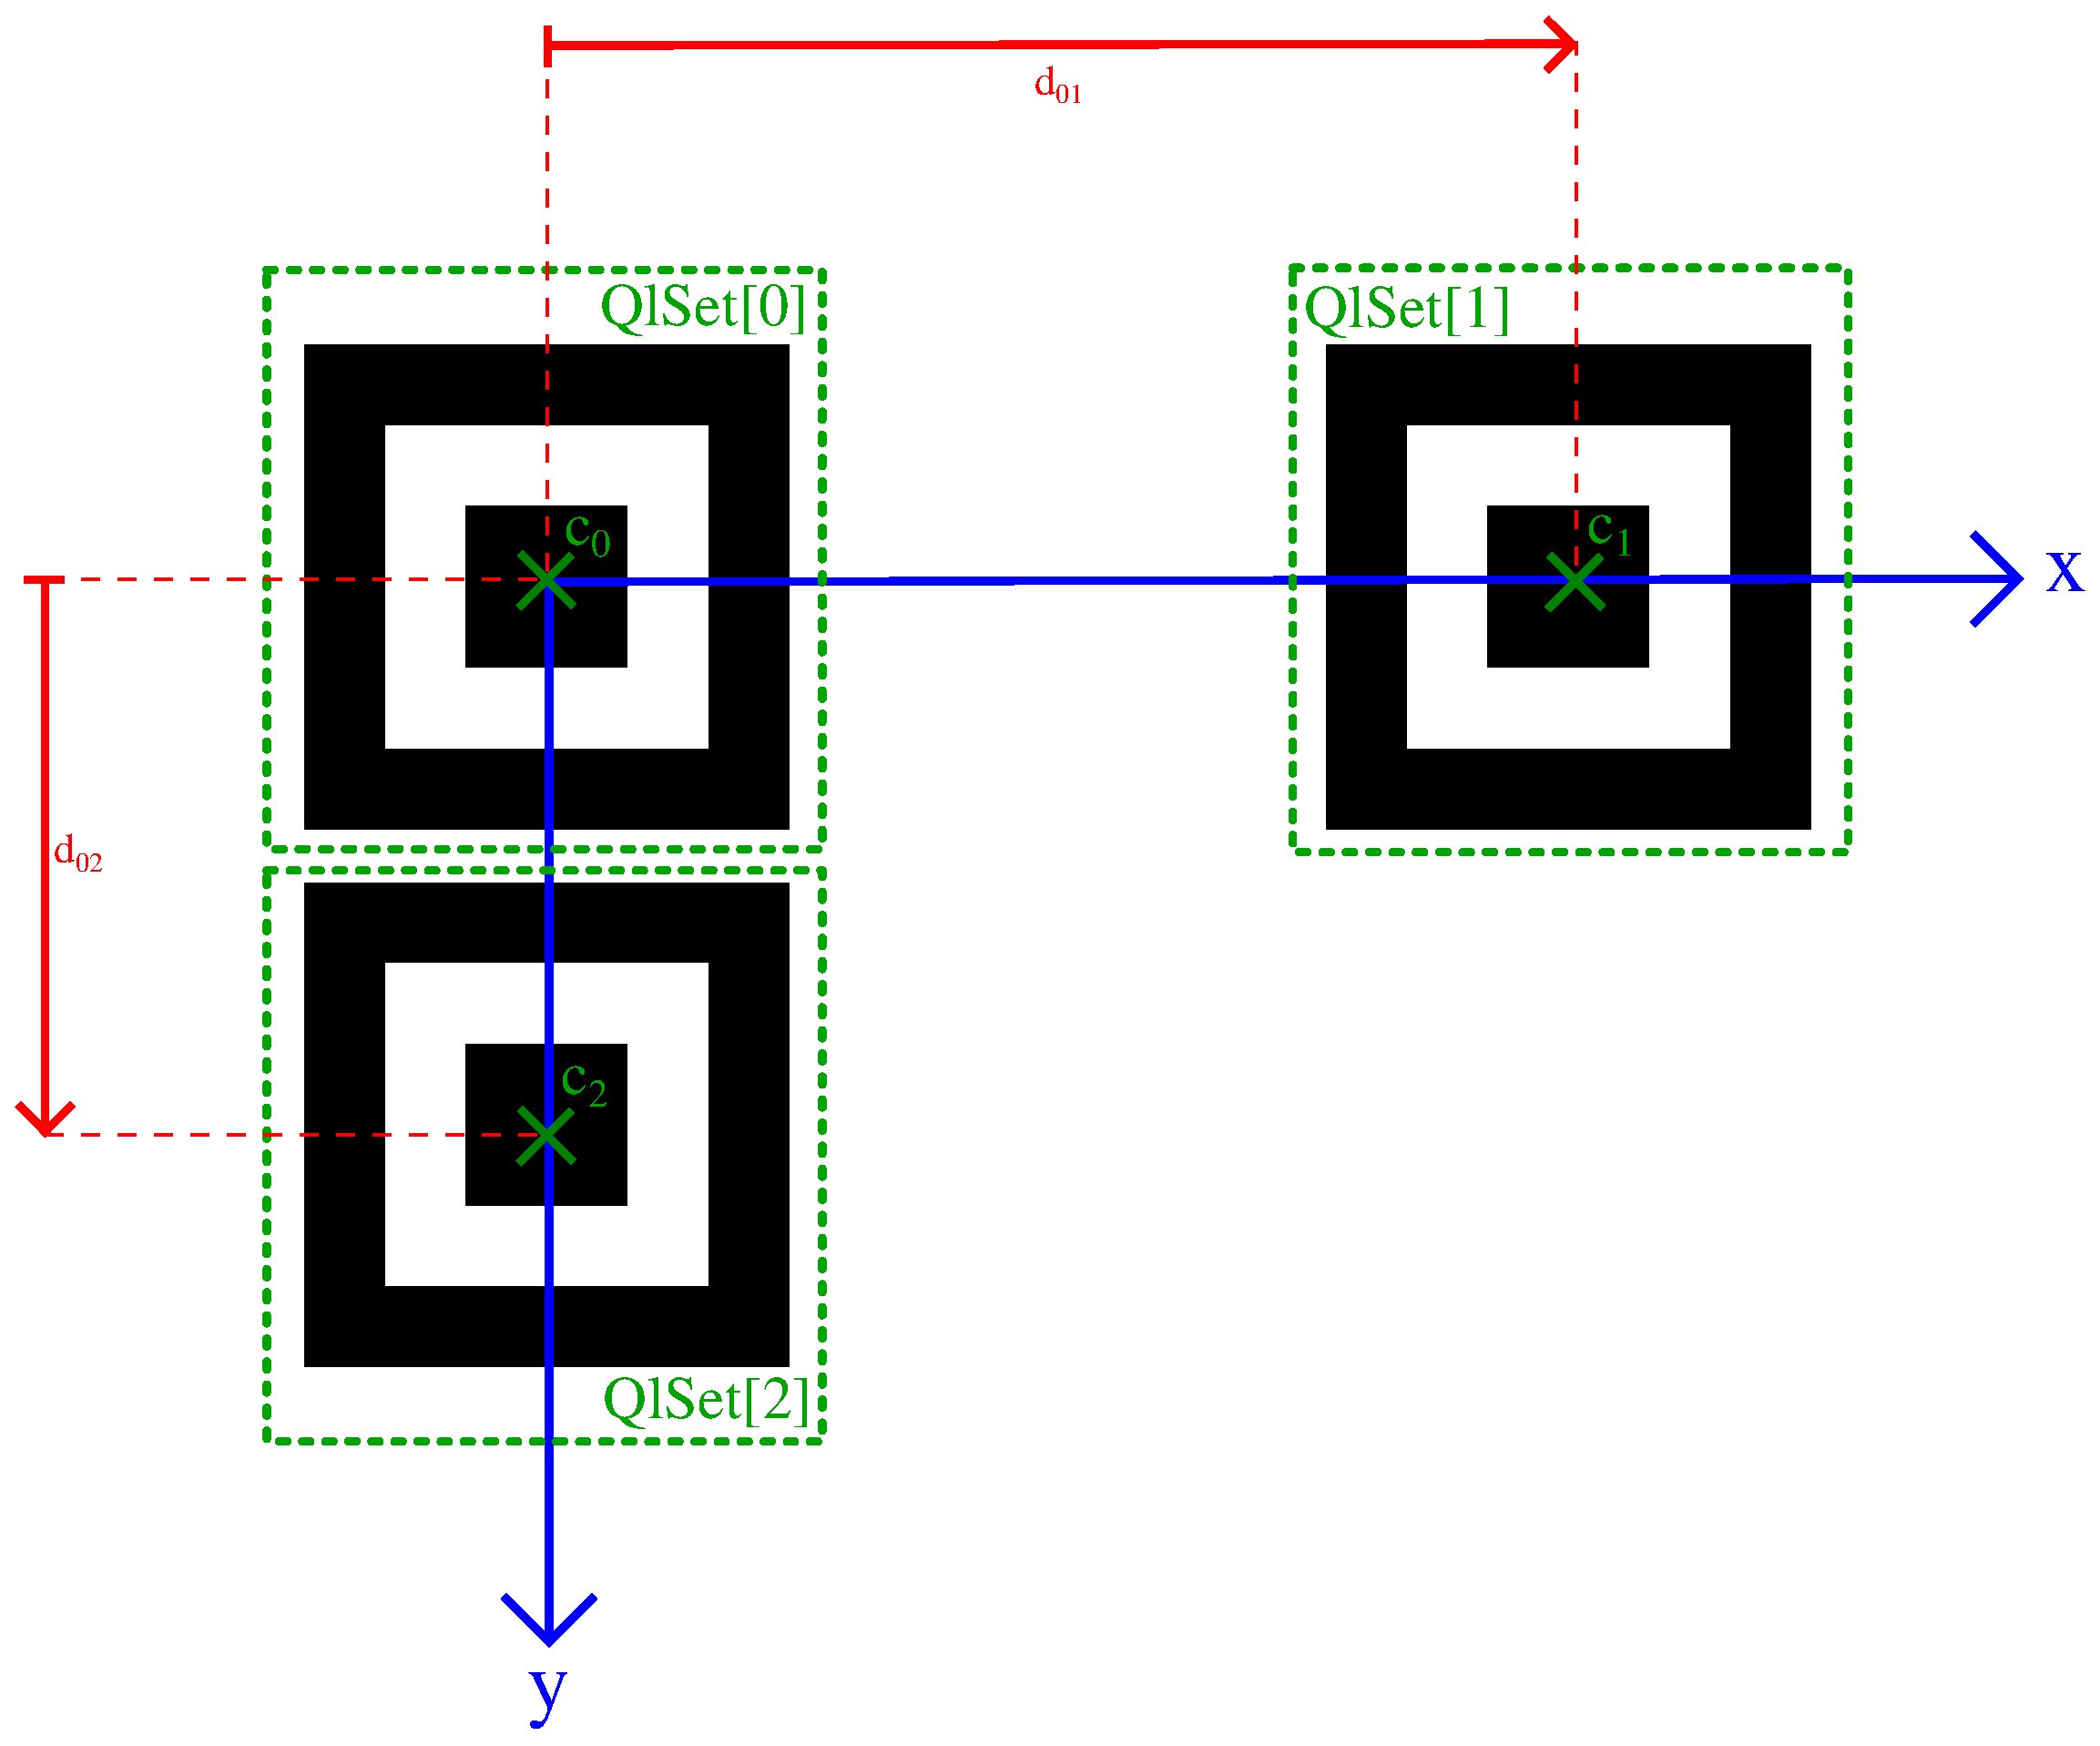
\includegraphics[scale=0.3]{figs_detection/MarkerDetail.eps}
\caption{Detalle del marcador propuesto formando un sistema de coordenadas.}
\label{fig:MarkerDetail}
\end{figure}


\subsection{Par�metros de dise�o}
Provisto el dise�o del marcador descrito, quedan definidos ciertos par�metros \textbf{estructurales} que fueron tomados fijos a lo largo del proyecto pero que podr�an ser cambiados para trabajos futuros asociados. Estos par�metros son:
\begin{itemize}
\item M: cantidad de conjuntos de cuadril�teros.
\item N: cantidad de cuadril�teros por conjuntos de cuadril�teros.
\item Geometr�a: geometr�a de los cuadril�teros ($Ql$).
\item Disposici�n: disposici�n espacial de los conjuntos de cuadril�teros ($QlSet$).
\end{itemize}

El criterio de elecci�n de $M$ y $N$ parte del dise�o los c�digos QR como ya fue explicado. La detecci�n por segmentos de l�nea resulta una cantidad de $3\times QlSet$'s conteniendo $3 \times Ql$'s cada uno. Bajo esta elecci�n de par�metros se tienen $36$ segmentos y v�rtices. Se tiene entonces un n�mero de puntos caracter�sticos razonable para la estimaci�n de pose.

La elecci�n de \emph{cuadrados} como par�metro de geometr�a se basa en la necesidad de tener igual resoluci�n en los dos ejes del marcador. De esta forma se asegura una distancia l�mite en donde, en un caso ideal enfrentado al marcador, la detecci�n de segmentos de l�nea falla simult�neamente en los segmentos verticales como en los horizontales. De otra forma se tendr�a una direcci�n que limita m�s que la otra desaprovechando resoluci�n.

La disposici�n espacial de los conjuntos de cuadril�teros esta en primer lugar limitada a un plano y en segundo lugar es tal que se puede definir ejes de coordenadas ortogonales mediante los centros como se muestra en la Figura \ref{fig:MarkerDetail}.\\

Por otro lado se tiene otro juego de par�metros \textbf{din�micos} que concluyen con el dise�o del marcador. Estos par�metros conservan la estructura intr�nseca del marcador permitiendo versatilidad en la aplicaci�n y sin la necesidad de modificaci�n alguna de los algoritmos desarrollados. Estos son:
\begin{itemize}
\item $d_{ij}$: distancia entre los centros $QlSet[j]$ con $QlSet[i]$.
\item $l$: lado del cuadril�tero m�s peque�o ($Ql[0]$) de los $QlSet$.
\end{itemize}

En este caso se debe cumplir siempre la condici�n impuesta previamente en donde $d_{01}\gg d_{02}$. De otra forma se deber�n realizar ciertas hip�tesis no gen�ricas o se deber� aumentar ligeramente la complejidad del algoritmo para la identificaci�n del marcador.\\

\subsection{Dise�o utilizado}
\textbf{Dise�o de Test}: Durante el desarrollo e implementaci�n de los algoritmos de detecci�n e identificaci�n de los v�rtices del marcador se trabaj� con determinados par�metros de dise�o de dimensiones apropiadas para posibilitar el traslado y las pruebas dom�sticas. 
\begin{itemize}
 \item $l = 30 mm$
 \item $d_{01} = 190 mm$
 \item $d_{02} = 100 mm$
\end{itemize}

\section{Detecci�n}
La etapa de detecci�n del marcador se puede separar en tres grandes bloques:
\begin{itemize}
 \item Detecci�n de segmentos de l�nea.
 \item Filtrado y agrupamiento de segmentos.
 \item Determinaci�n de correspondencias.
\end{itemize}
En esta secci�n se muestran algunos resultados para la detecci�n de segmentos de l�nea por LSD y se centra en profundidad en los algoritmos desarrollados durante el proyecto para el filtrado de segmentos y determinaci�n de correspondencias.

\subsection{Detecci�n de segmentos de l�nea}
La detecci�n de segmentos de l�nea se realiza mediante el uso del algoritmo LSD el cual se detalla en el Cap�tulo \ref{chap: lsd}. En forma resumida, dicho algoritmo toma como entrada una imagen en escala de grises de tama�o $W\times H$ y devuelve una lista de segmentos en forma de pares de puntos de origen y destino. 

En la Figura \ref{fig:resultado_lsd} se muestra un resultado para la detecci�n de segmentos de l�nea por LSD.
\begin{figure}[h!]
  \centering
  \subfigure[Entrada: imagen conteniendo al marcador]{
    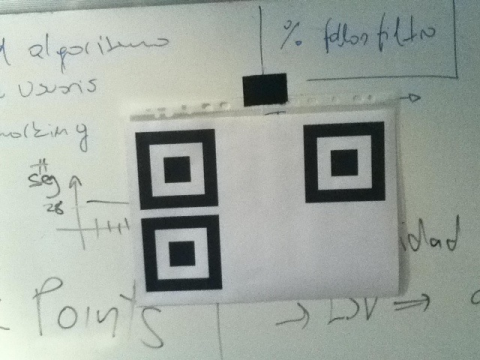
\includegraphics[scale=0.45]{figs_detection/img.png}}
  \subfigure[Salida: segmentos de l�nea detectados por LSD]{
    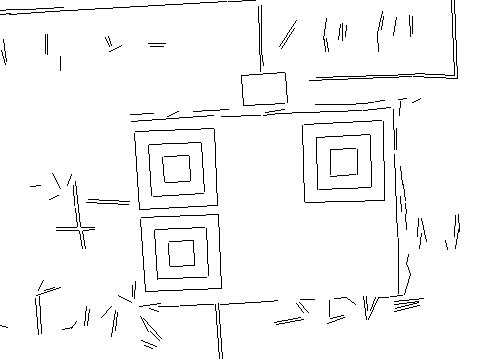
\includegraphics[scale=0.45]{figs_detection/lsd.png}}
  \caption{Resultados del algoritmo de detecci�n de segmentos de l�nea LSD.}
  \label{fig:resultado_lsd}
\end{figure}

\subsection{Filtrado y agrupamiento de segmentos}
El filtrado y agrupamiento de segmentos consiste en la b�squeda de conjuntos de cuatro segmentos conexos en la lista de segmentos de l�nea detectados por LSD. Los conjuntos de segmentos conexos encontrados se devuelven en una lista en el mismo formato a la de LSD pero agrupados de a cuatro. A continuaci�n se realiza una breve descripci�n del algoritmo de filtrado de segmentos implementado.\\

Se parte de una lista de $m$ segmentos de l�nea,
\begin{equation}
 \mathbf{L} = \begin{pmatrix}
               \mathbf{s}_0 & \mathbf{s}_1 & \dots & \mathbf{s}_{m-1} 
              \end{pmatrix}^t
\end{equation}
y se recorre en $i$ en busca de segmentos vecinos. La estrategia utilizada consiste en buscar, para el $i$-�simo segmento $\mathbf{s}_i$, dos segmentos vecinos. En una primera etapa $\mathbf{s}_j$ y en una segunda etapa $\mathbf{s}_k$, de forma que se forme una ``U'' como se muestra en la Figura \ref{fig:SegmentosRectas}. La tercer etapa de b�squeda consiste en completar ese conjunto con un cuarto segmento $\mathbf{s}_l$ que cierre la ``U''.

Dos segmentos $\mathbf{s}_i$ y $\mathbf{s}_j$ son vecinos si se cumple que la distancia eucl�dea entre puntos, $d_{ij}$, es menor a un cierto umbral para alguna de las combinaciones $\mathbf{p}_i\leftrightarrow \mathbf{p}_j$, $\mathbf{q}_i\leftrightarrow \mathbf{q}_j$, $\mathbf{p}_i\leftrightarrow \mathbf{q}_j$ o $\mathbf{q}_i\leftrightarrow \mathbf{p}_j$. En la primera etapa de la b�squeda se testean todas las posibilidades mientras que en la segunda etapa se testean solo los puntos del segmento que no fueron utilizados. Por ejemplo, si se encontr� la correspondencia $\mathbf{p}_i\leftrightarrow \mathbf{p}_j$ se busca el $k$-�simo segmento $\mathbf{s}_k$ que cumple que la distancia euclidiana $d_{ij}$ es menor a cierto umbral para alguna de las combinaciones $\mathbf{q}_i\leftrightarrow \mathbf{p}_k$ y $\mathbf{q}_i\leftrightarrow \mathbf{q}_k$. En la tercer etapa la chequeo se realiza de forma a�n m�s restringida probando para el segmento $\mathbf{s}_l$ correspondencia simult�nea entre sus puntos y solamente un punto cada uno de los segmentos $\mathbf{s}_j$ y $\mathbf{s}_k$ .\\
\begin{figure}[h!]
\centering
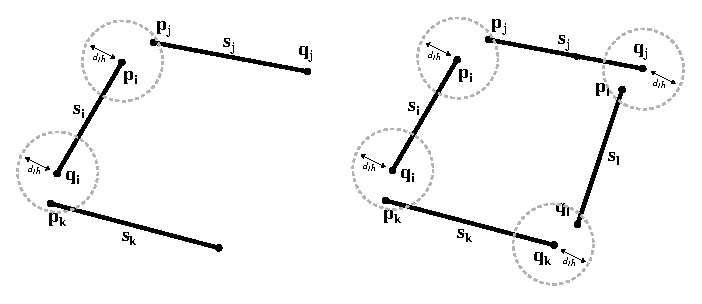
\includegraphics[scale=0.8]{figs_detection/SegmentosRectas.eps}
\caption{Conjunto de cuadril�teros conexos. A la izquierda la primera y segunda etapa del filtrado completadas para el segmento $\mathbf{s}_i$ en donde se busca una ``U''. A la derecha la �ltima etapa en donde se cierra la ``U'' con el segmento $\mathbf{s}_l$.}
\label{fig:SegmentosRectas}
\end{figure}

Una vez encontrado el conjunto de cuatro segmentos conexos estos se marcan como utilizados, se guardan en una lista de salida y se contin�a con el segmento $i+1$ hasta recorrer los $m$ segmentos de la lista de entrada. De esta forma se obtiene una lista de salida $\mathbf{S}$ de $n$ segmentos en donde $n$ es por construcci�n m�ltiplo de cuatro.\\

En la Figura \ref{fig:resultado_lsdfilt} se muestran lo resultados obtenidos para el algoritmo tomando como entrada la lista de segmentos de LSD. Se puede ver que los lados de los cuadrados del marcador son detectados correctamente pero tambi�n hay otras detecciones presentes. Por ejemplo el rect�ngulo negro correspondiente a un trozo de cinta negra que sostiene el marcador (ver Figura \ref{fig:resultado_lsd}(a)). Tambi�n sobreviven otro tipo de elementos indeseados que se explican a continuaci�n.
\begin{figure}[h!]
  \centering
  \subfigure[Entrada: segmentos de l�nea detectados por LSD]{
    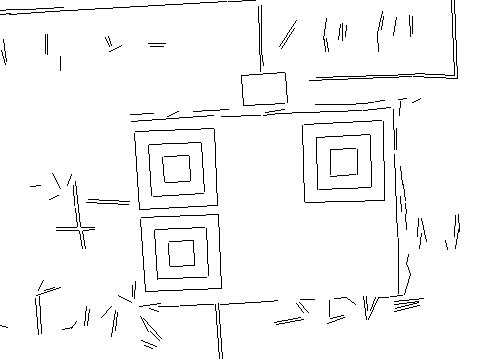
\includegraphics[scale=0.45]{figs_detection/lsd.png}}
  \subfigure[Salida: segmentos de l�nea filtrados y agrupados]{
    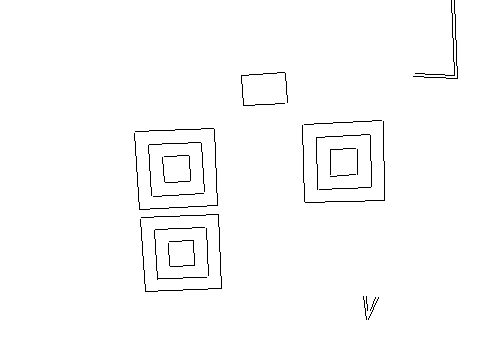
\includegraphics[scale=0.45]{figs_detection/lsdfilt.png}}
  \caption{Resultados del algoritmo de filtrado y agrupamiento de segmentos de l�nea.}
  \label{fig:resultado_lsdfilt}
\end{figure}

El algoritmo descrito es simple y provee resultados aceptables en general pero es propenso a tanto a detectar \emph{falsos positivos} como al \emph{sobre-filtrado} algunos conjuntos. 

La detecci�n de falsos positivos se puede atribuir principalmente a la condici�n de vecindad utilizada en donde un caso como el que se muestra en la Figura \ref{fig:FilterError} de un conjunto de segmentos paralelos cercanos y de tama�o similar ``sobrevive'' al filtrado de segmentos. De forma de evitar estos  falsos positivos, se podr�a considerar implementar un condici�n de vecindad que tome en cuenta el punto de  intersecci�n entre los segmentos y la distancia de este punto a los puntos $\mathbf{p}$, $\mathbf{q}$ m�s cercanos de cada segmento. Como se explicar� en le Secci�n \ref{sec:detection_correspondencias}, debido a que el algoritmo de determinaci�n de correspondencias realiza la intersecci�n entre estos segmentos se puede chequear alguna condici�n sobre los segmentos o su intersecci�n y en ese momento filtrar estos casos.
\begin{figure}[h!]
\centering
\includegraphics[scale=0.8]{figs_detection/FilterError.eps}
\caption{Posible configuraci�n de segmentos paralelos que ``sobreviven'' al filtrado. A la izquierda el grupo de segmentos, a la derecha se muestra como se desarrolla el filtrado de $\mathbf{s}_i$.}
\label{fig:FilterError}
\end{figure}

El sobre-filtrado de segmentos tiende a ocurrir cuando no se cumple la condici�n de distancia entre segmentos vecinos cuando visualmente si lo son. Se debe principalmente a que se utiliza para el filtrado un valor de $d_{th}$ fijo que conduce a buenos resultados para la aplicaci�n pero en ciertas circunstancias produce este problema. Esta medida de distancia se podr�a tomar relativa al largo del los segmentos a \emph{testear} de forma de generalizar el valor pero se deber�a analizar un poco m�s en detalle la posible implementaci�n para que resulte en buenos resultados y no introduzca otra clase de errores.\\

El algoritmo de filtrado y agrupamiento de segmentos es sensible respecto a la elecci�n del par�metro $d_{th}$. Si este par�metro est� por debajo del valor �ptimo la \emph{performance} del algoritmo se ver� afectada fuertemente, pues se corre el riesgo de sobre filtrar y no proporcionar suficientes segmentos para la correcta determinaci�n de correspondencias. Por el contrario, si el par�metro est� por encima del valor �ptimo, el filtrado tiende a proveer falsos positivos, aunque este caso no llega a ser tan cr�tico como el primero para la aplicaci�n. A modo de ejemplo, para una imagen de tama�o $480 \times 320$ con el marcador ocupando entre un $25\%$ y un $80\% $ el valor del par�metro que da mejores resultados es aproximadamente de $6$ o $7$ p�xeles.

\subsection{Determinaci�n de correspondencias}
\label{sec:detection_correspondencias}
Se detalla a continuaci�n el algoritmo de determinaci�n de correspondencias a partir de grupos de cuatro segmentos de l�nea conexos. Para ese algoritmo se hace uso de los elementos estructurales del marcador vistos en la Secci�n \ref{sec:detection_estructuras}, de forma de desarrollar un algoritmo modular, escalable y simple.

Se toma como entrada la lista de segmentos filtrados y agrupados
\begin{equation}
\mathbf{S} = \begin{pmatrix}
			 \mathbf{s}_0 & \mathbf{s}_1 & \dots & \mathbf{s}_{i} & \mathbf{s}_{i+1} & \mathbf{s}_{i+2} & \mathbf{s}_{i+3} & \dots & \mathbf{s}_{n-1}
			 \end{pmatrix}^t
\end{equation}
en donde cada segmento se compone de un punto inicial $\mathbf{p}_{i}$ y un punto final $\mathbf{q}_{i}$, $\mathbf{s}_{i} = (\mathbf{p}_{i},\mathbf{q}_{i})$, con $n$ m�ltiplo de cuatro. Si $i$ tambi�n lo es, entonces el sub-conjunto, 
$\mathbf{S}_i = \begin{pmatrix}
				\mathbf{s}_{i} & \mathbf{s}_{i+1} & \mathbf{s}_{i+2} & \mathbf{s}_{i+3}
				\end{pmatrix}^t$, corresponde a un conjunto de cuatro segmentos del l�nea conexos.

Para cada sub-conjunto $\mathbf{S}_i$ se intersectan entre s� los segmentos obteniendo una lista de cuatro v�rtices,
$\mathbf{V}_i =  \begin{pmatrix}
		 \mathbf{v}_{i} & \mathbf{v}_{i+1} & \mathbf{v}_{i+2} & \mathbf{v}_{i+3} 
		 \end{pmatrix}^t$. 
Si  $\mathbf{r}_i$ es la recta que pasa por los puntos $\mathbf{p}_i$ y $\mathbf{q}_i$ del segmento  $\mathbf{s}_i$, la lista de v�rtices se obtiene como sigue,
\begin{eqnarray}
\mathbf{v}_i = & \mathbf{r}_i\cap \mathbf{r}_{i+1} \nonumber\\
\mathbf{v}_{i+1} = & \mathbf{r}_i\cap \mathbf{r}_{i+2} \nonumber\\
\mathbf{v}_{i+2} = & \mathbf{r}_{i+3}\cap \mathbf{r}_{i+2} \nonumber\\
\mathbf{v}_{i+3} = & \mathbf{r}_{i+3}\cap \mathbf{r}_{i+1} \nonumber
\end{eqnarray}
resultando en dos posibles configuraciones de v�rtices. Las dos configuraciones se muestran en la Figura \ref{fig:Vertices} en donde una de ellas tiene sentido horario y la otra antihorario partiendo de ${v}_i$.
\begin{figure}[h!]
\centering
\includegraphics[scale=0.8]{figs_detection/Vertices.eps}
\caption{Posibles configuraciones de v�rtices posterior a la intersecci�n de conjuntos de segmentos pertenecientes a un cuadril�tero.}
\label{fig:Vertices}
\end{figure}

Posterior a la intersecci�n se realiza un chequeo sobre el valor de las coordenadas de los v�rtices. Si alguno de ellos se encuentra fuera de los l�mites de la imagen, el conjunto de cuatro segmentos es marcado como inv�lido. Este chequeo resulta en el filtrado de ``falsos cuadril�teros'' corrigiendo un defecto del filtrado de segmentos, como por ejemplo un grupo de segmentos paralelos cercanos como ya se explic�. 

Para cada uno de los conjuntos de v�rtices se construye con ellos un elemento cuadril�tero que se almacena en una lista de cuadril�teros
\begin{eqnarray*}
 QlList =  \begin{pmatrix}
            Ql[0] & Ql[1] & \dots & Ql[i] & \dots & Ql[\frac{n}{4}]
           \end{pmatrix}^t
\end{eqnarray*}
% en sentido amplio, de dos segmentos contiguos, $s_i\cap s_{i+1}$ dadas las recta $r_1$ que pasa por los puntos $\mathbf{p}_1$, $\mathbf{q}_1$ del segmento $s_1$ y la recta $r_2$ que pasa por los puntos $\mathbf{p}_2$, $\mathbf{q}_2$ del segmento $s_2$, se determina el v�rtice correspondiente como la intersecci�n $r_1 \cap r_2$. \\
% 
% y se intersectan en grupos de cuatro obteniendo cuatro v�rtices por cada grupo. Para cada grupo de v�rtices $v_k$ se construye un elemento cuadril�tero $\text{Ql}[k]$ que se almacena en una lista de cuadril�teros. 

A partir de esa lista de cuadril�teros, se buscan grupos de tres cuadril�teros $QlSet$ que ``compartan'' un mismo centro. Para esto se recorre ordenadamente la lista en $i$ buscando para cada cuadril�tero dos cuadril�teros $j$ y $k$ que cumplan que la distancia entre sus centros  y el del $i$-�simo cuadril�tero sea menor a cierto umbral $c_{th}$,
\begin{equation}
\begin{split}
 d_{ij} = ||\mathbf{c}_i - \mathbf{c}_j||<c_{th}, & \quad  d_{ik} = ||\mathbf{c}_i - \mathbf{c}_k||<c_{th}.
\end{split}
\end{equation}
Estos cuadril�teros se marcan en la lista como utilizados con ellos se forma el $l$-�simo $QlSet$ orden�ndolos seg�n su per�metro, de menor a mayor como  
$$QlSet[l] = \begin{pmatrix} Ql[0] & Ql[1] & Ql[2] \end{pmatrix}$$
con $l = (0,1,2)$. Esta b�squeda se realiza hasta encontrar un total de tres $QlSet$ completos de forma de obtener un marcador completo, esto es, detectando todos los cuadril�teros que lo componen. \\

Una vez obtenida la lista de tres $QlSet$, 
$$QlSetList = \begin{pmatrix} QlSet[0] & QlSet[1] & QlSet[2] \end{pmatrix}$$
�sta se ordena de forma que su disposici�n espacial se corresponda con la del marcador QR. Para esto se calculan las distancias entre los centros de cada $QlSet$ y se toma el �ndice $i$ como el �ndice que produce el vector de menor distancia, $\mathbf{u}_i = \mathbf{c}_{i+1} -\mathbf{c}_i$. En este punto es importante que la condici�n de distancia entre los centros de los $QlSet$ se cumpla, $d_{10} \gg d_{20}$, para una simple identificaci�n. Bajo una transformaci�n proyectiva del marcador, es posible que esta relaci�n se modifique e incluso que deje de valer, pero imponiendo la condici�n ``mucho mayor'' se asegura que el algoritmo funciona correctamente para condiciones razonables. Esto es, para proyecciones o poses que se encuentran dentro de las hip�tesis de uso de la aplicaci�n.

Una vez seleccionado el vector $\mathbf{u}_i$, se tienen obtiene el juego de vectores $(\mathbf{u}_i,\mathbf{u}_{i+1},\mathbf{u}_{i+2})$ como se muestra en la figura \ref{fig:Centros}.
\begin{figure}[h!]
\centering
\includegraphics[scale=0.45]{figs_detection/Centros.eps}
\caption{V�rtices de cada $Ql$ ordenados respecto al signo de sus proyecciones contra el sistema de coordenadas local a cada $QlSet$.}
\label{fig:Centros}
\end{figure}

Existen solo dos posibles configuraciones para estos vectores por lo que se utiliza este conocimiento para ordenar los $QlSet$ de la lista realizando el producto vectorial, aumentando la dimensi�n de los vectores $\hat{\mathbf{u}_i}$ y $\hat{\mathbf{u}_{i+1}}$ con coordenada $z=0$,
\begin{equation*}
 \mathbf{b} = \hat{\mathbf{u}_i} \times \hat{\mathbf{u}_{i+1}}.
\end{equation*}
Si el vector $\mathbf{b}$ tiene valor en la coordenada $z$ positivo se ordena como,
\begin{eqnarray*}
 QlSet[0]\longleftarrow & QlSet[i]\\
 QlSet[1]\longleftarrow & QlSet[i+2]\\
 QlSet[2]\longleftarrow & QlSet[i+1]
\end{eqnarray*}
o de lo contrario se ordena como,
\begin{eqnarray*}
 QlSet[0]\longleftarrow & QlSet[i+1]\\
 QlSet[1]\longleftarrow & QlSet[i+2]\\
 QlSet[2]\longleftarrow & QlSet[i]
\end{eqnarray*}

Por ultimo se construye un marcador QR que contiene la lista de tres $QlSet$ ordenados seg�n lo indicado permitiendo la definici�n de un centro de coordenadas como el centro $\mathbf{c}_0$ del $QlSet[0]$ y ejes de coordenadas definidos en la Ecuaci�n \ref{ec:detection_ejes}. Los ejes de este sistema de coordenadas permiten, para cada $Ql$ de cada $QlSet$, proyectar los v�rtices sobre el sistema de coordenadas local al $QlSet$ y seg�n su signo ordenarlos como se muestra en la Figura \ref{fig:VerticesProyectados}.
\begin{figure}[h!]
\centering
\includegraphics[scale=0.8]{figs_detection/VerticesProyectados.eps}
\caption{Posibles configuraciones de centros resultan en la orientaci�n de los vectores $\mathbf{u}_{i+k}$.}
\label{fig:VerticesProyectados}
\end{figure}
De esta forma, recorriendo ordenadamente los elementos del marcador, se ordenan los v�rtices de cada $Ql$ del marcador.\\

Por �ltimo, a partir del marcador ordenado, se extrae una lista de v�rtices que se corresponde con la lista de v�rtices del marcador en coordenadas del mundo. Este recorrido se realiza en el siguiente orden,
\begin{algorithm}
\For{$i=(0,1,2)$}
  { \For{$j=(0,1,2)$}
  { \For{$k=(0,1,2,3)$} {
    So obtiene el punto v�rtice: $\mathbf{p} = QlSet[i] \rightarrow Ql[j] \rightarrow v[k]$\;
    Se agrega a la lista de correspondencias $\mathbf{m}_{l} \leftarrow \mathbf{p}$\;
    Se incrementa $l$;
  }}}
\end{algorithm}

Se determinan las correspondencias $\mathbf{M}_i\leftrightarrow \mathbf{m}_i$ necesarias para la estimaci�n de pose las cuales se muestran en la Figura \ref{fig:resultado_points}. Se puede ver que el algoritmo de determinaci�n de correspondencias funciona correctamente por lo que los ``falsos'' cuadril�teros que sobreviven al filtrado de segmentos no son un problema.
\begin{figure}[h!]
  \centering
  \subfigure[Entrada: segmentos de l�nea filtrados y agrupados]{
    \includegraphics[scale=0.45]{figs_detection/lsdfilt.png}}
  \subfigure[Salida: puntos v�rtices ordenados.]{
    \includegraphics[scale=0.45]{figs_detection/points.png}}
  \caption{Resultados del algoritmo de determinaci�n de correspondencias.}
  \label{fig:resultado_points}
\end{figure}

\subsection{Detecci�n robusta}
El algoritmo descripto al momento requiere que dentro de la lista de segmentos filtrados se encuentren todos los segmentos que componen el marcador pero este requerimiento representa un problema importante en cuanto a el desempe�o del algoritmo. En caso de que esto no se cumpla no es posible proporcionar las correspondencias necesarias para la estimaci�n de pose y no se tendr� una pose v�lida para ese cuadro o \emph{frame} para la aplicaci�n. En aplicaciones en tiempo real en donde el procesamiento de la imagen es la mayor limitante, la fluidez visual dada por el \emph{frame rate} se ve notablemente perjudicada resultando en que el sistema sea inc�modo e incluso inutilizable. Es por esto que en esta secci�n se desarrolla la extensi�n del algoritmo de determinaci�n de correspondencias para una cantidad menor de segmentos detectados y filtrados que resulta en una mejora sustancial en la cantidad de \emph{frames} en los cuales es posible determinar correspondencias y obtener as� una pose v�lida.

Se busca una determinaci�n de correspondencias m�s robusta pero manteniendo las esencia del algoritmo desarrollado. Por esto se tienen dos aspectos a tomar en cuenta; la detecci�n de $QlSet$'s se realiza basada en la b�squeda de cuadril�teros conc�ntricos por lo que se debe contar con un m�nimo de dos cuadril�teros por $QlSet$ para permitir la diferenciaci�n entre un conjunto de segmentos filtrados debido a que pertenecen al marcador y a otro conjunto que no pertenece pero si cumple con las condiciones, por ejemplo podr�a ser el marco de una obra o cualquier elemento en la escena que forme un cuadril�tero. Esto fija un l�mite de no menos de $24$ segmentos necesarios para el funcionamiento. El otro aspecto a tomar en cuenta se refiere a la forma en que se ordenan los $Ql$'s dentro de cada $QlSet$. Como ya se explic� el orden se basa en la medida del per�metro de los $Ql$'s ordenando de menor a mayor por lo que ser� necesario contar con, al menos, un $QlSet$ completo de forma de tener una referencia a la hora de identificar los $QlSet$'s incompletos hallados. Por lo tanto la extensi�n del algoritmo permite una correcta identificaci�n de los v�rtices del marcador con un n�mero mayor o igual a $28$ segmentos.\\

La implementaci�n de esta extensi�n del algoritmo se realiz� manteniendo la estructura b�sica descrita anteriormente y se detalla aqu� solamente los agregados realizados.

Al realizar la b�squeda de conjuntos de cuadril�teros conc�ntricos se buscan en primer lugar los $QlSet$'s completos y luego en caso de que estos no lleguen a ser tres, se intenta completar buscando $QlSet$'s incompletos o sea conjuntos de dos cuadril�teros que comparten un mismo centro. Estos se agrupan en una lista de la misma forma en que se describi� anteriormente pero dejando el tercer cuadril�tero, $Ql[2]$, marcado como inv�lido.

Una vez completada la lista de tres $QlSet$, con al menos uno de ellos detectado completo, se ordenan en primer lugar los $QlSet$ completos y de ellos se extrae una lista de per�metros promedio. Esta lista de per�metros promedio se utiliza para el ordenamiento de los $QlSet$ incompletos comparando con los per�metros de los $Ql[0]$ y $Ql[1]$ de cada $QlSet$. El $Ql[2]$ previamente marcado como inv�lido se posiciona por descarte en la posici�n que corresponda.

Al momento de proporcionar la lista de v�rtices ordenados $\mathbf{m}_i$ y correspondientes con los del modelo $\mathbf{M}_i$, se introducen valores inv�lidos para los $Ql$'s marcados como inv�lidos. Por �ltimo se realiza un recorte de las dos listas de puntos en base a estos valores inv�lidos, se recorre la lista de puntos en la imagen $\mathbf{m}_i$ y se extraen de la lista de puntos en la imagen y de los puntos del modelo los puntos inv�lidos obteniendo un juego de al menos $28$ correspondencias $\mathbf{m}_i' \leftrightarrow \mathbf{M}'_i$ para el algoritmo de estimaci�n de pose.\\

En la Figura \ref{fig:resultado_inc_points}(a) se muestran imagen en la que falla el filtrado de segmentos para uno de los cuadril�teros mientras que en la figura \ref{fig:resultado_inc_points}(b) se puede ver como el algoritmo de determinaci�n de correspondencias provee $32$ correspondencias ordenadas correctamente, diferenciando en el $QlSet$ incompleto los v�rtices.
\begin{figure}[h!]
  \centering
  \subfigure[Entrada: segmentos de l�nea filtrados y agrupados]{
    \includegraphics[scale=0.45]{figs_detection/mrkr_incompleto/lsdfilt.png}}
  \subfigure[Salida: puntos v�rtices ordenados.]{
    \includegraphics[scale=0.45]{figs_detection/mrkr_incompleto/points.png}}
  \caption{Resultados del algoritmo de determinaci�n de correspondencias robusto para una falla en el filtrado de segmentos.}
  \label{fig:resultado_inc_points}
\end{figure}

% La detecci�n de segmentos puede fallar debido a que las dimensiones del marcador en el plano de imagen sean peque�as y que la detecci�n de segmentos deje de ser estable. Tambi�n debido a oclusiones o ``segmentos'' partidos. Por otro lado debido a la simplicidad del algoritmo de filtrado y agrupamiento de segmentos, en particular debido simplicidad de la condici�n de vecindad, el algoritmo es propopenso a fallas por ejemplo filtrando un conjunto de cuatro segmentos cuando en la detecci�n de segmentos se puede ver que estan all�. puede fallar.

\section{Comentarios sobre la implementaci�n de los algoritmos}
Los algoritmos desarrollados en el presente cap�tulo fueron implementados en Lenguaje C y est�n autocontenidos en el mismo c�digo fuente sin la utilizaci�n de librer�as externas para su funcionamiento.\\

La elecci�n del lenguaje y la filosof�a de desarrollo comentada atr�s permite \textbf{portabilidad} en el uso de los mismos para aplicaciones m�s all� del proyecto y es un ejercicio de aprendizaje necesario. El algoritmo de filtrado y agrupamiento se implement� en los archivos \texttt{segments.c} y \texttt{segments.h} mientras que el de determinaci�n de correspondencias se implement� en los archivos \texttt{marker.c} y \texttt{marker.h}.\\

El entorno de desarrollo (IDE) utilizado para la implementaci�n fue Eclipse CDT para C/C++: \url{http://www.eclipse.org/cdt/} en un proyecto que utiliza un \emph{Makefile} para la compilaci�n por lo que se podr�a utilizar otro entorno en caso de ser necesario.\\

Adicionalmente de forma de facilitar la tareas de interfaz como el abrir/capturar, el guardado/despliegue de im�genes o video as� como el dibujado de segmentos y puntos sobre las im�genes se utiliza la librer�a OpenCV. Se aclara que esta interfaz no est� de ninguna forma integrada con los algoritmos desarrollados pero fue de gran utilidad para la implementaci�n de los mismos. Su utilizaci�n esta intr�nsecamente ligada a la librer�a OpenCV pero esta es una muy popular librer�a multifplataforma para procesamiento de im�genes.

\section{Resultados de Benchmark}
En esta secci�n se presentan algunos resultados de \emph{Benchmark} para los algoritmos de asociados a la detecci�n del marcador dise�ado. En particular se estudian los l�mites para la detecci�n de segmentos mediante LSD y el filtrado y agrupamiento de los mismos para juegos de im�genes sint�ticas generadas utilizando las herramientas explicadas en el Cap�tulo \ref{chap: benchmark}.\\

Se analizan los casos que presentaron limitaciones m�s significativas como, la profundidad m�xima del marcador respecto al eje $z$, la rotaci�n m�xima permitida sobre el eje $x$ y lo mismo para la rotaci�n sobre el eje $y$. Mediante este an�lisis se obtienen cotas \emph{pseudo-te�ricas} para establecer las limitaciones pr�cticas de uso de los algoritmos.\\

\subsection{Elecci�n de par�metros para Benchamark}
Para la evaluaci�n de los algoritmos se utilizaron algunos par�metros de Benchmark fijos y otros modificables llevando a una elecci�n definitiva de par�metros.\\

Un juego de par�metros fue tomado fijo y se refiere a la c�mara utilizada. 
\begin{itemize}
 \item $width \times height$: Tama�o de imagen tomado $480\times360$.
 \item $fov$: Campo visual referido al ancho tomado $46.46�$
 \item $centro$: Centro de la c�mara siempre ubicado en el medio de la imagen.
\end{itemize}

A lo largo de las diferentes pruebas realizadas se probaron modificar algunos par�metros para ver como estos afectaban los resultados. Los par�metros modificables son:
\begin{itemize}
 \item $d_{th}$: Distancia del threshold de filtrado de segmentos.
 \item $s$: Escala del LSD.
 \item $width \times height$: Tama�o de imagen.
\end{itemize}
Los valores que toman estos par�metros para las pruebas finales que corresponden con las que se muestran:
\begin{itemize}
 \item $d_{th} = 5px$
 \item $s = 0.5$
 \item $width\times height = 480\times360 px$
\end{itemize}
La elecci�n de estos par�metros fue \textbf{definitiva} para las pruebas de Benchmark a lo largo de todo el documento. Por m�s informaci�n sobre las herramientas de Benchmark y los par�metros ajustables para la generaci�n de im�genes sint�ticas referirse al Cap�tulo \ref{chap: benchmark}.

\newpage
\subsection{L�mite en profundidad: Eje z}
Para realizar las pruebas del l�mite de profundidad del marcador se gener� un juego de im�genes (\emph{Caso 1}) en las cuales el marcador se ubica enfrentado a la c�mara con el centro del mismo coincidente con el centro �ptico de la c�mara y por lo tanto en el centro de la imagen. Se utilizan profundidades que var�an desde $z=600mm$ hasta $z=2100mm$ de a $1mm$. \\

Se puede ver en la Figura \ref{fig:benchmark_segmentos_z} los casos l�mite sobre el cual el LSD no provee resultados satisfactorios y tambi�n el caso l�mite inmediatamente anterior a la falla del filtrado de segmentos. Se puede concluir que para el caso de profundidad el detector de segmentos LSD limita primero a una distancia de $z=1575mm$.
\begin{figure}[H]
  \centering
  \subfigure[Resultado de LSD para $z= 1575 mm$]{
    \includegraphics[scale=0.48]{figs_detection/limitesDeteccion/Caso1-LSD196.png}}
  \subfigure[Resultado de LSD para $z= 1580 mm$]{
    \includegraphics[scale=0.48]{figs_detection/limitesDeteccion/Caso1-LSD197.png}}
  \subfigure[Resultado de filtrado de segmentos para $z= 1575 mm$]{
    \includegraphics[scale=0.48]{figs_detection/limitesDeteccion/Caso1-LSDfilter196.png}}
  \caption{L�mites para la profundidad m�xima en el eje $z$ del marcador.}
  \label{fig:benchmark_segmentos_z}
\end{figure}

\newpage
\subsection{L�mite en rotaci�n: Eje x}
Para las pruebas del l�mite de rotaci�n sobre el eje $x$ del marcador se gener� un juego de im�genes (\emph{Caso 3}) en las cuales el marcador se ubica a una distancia fija de $z=1000mm$ con el centro del mismo coincidente con el centro �ptico de la c�mara y por lo tanto en el centro de la imagen. Sobre esta traslaci�n se varia la rotaci�n en el eje $x$ de a $2�$ desde $r_x = -60�$ hasta $r_x = 60�$.\\

Se puede ver en las Figuras \ref{fig:benchmark_segmentos_rx}(a) y \ref{fig:benchmark_segmentos_rx}(b) los casos de l�mite negativos y positivos respectivamente en los cuales el LSD falla. Debido a la asimetr�a del marcador limitan primero las rotaciones negativas. Por otro lado en las Figuras \ref{fig:benchmark_segmentos_rx}(c) y  \ref{fig:benchmark_segmentos_rx}(d) se observan los casos de l�mite negativos y positivos respectivamente inmediatamente anteriores a la falla del filtrado de segmentos. Se puede concluir que para las rotaciones sobe el eje $x$ limita LSD ya que el filtrado de segmentos funciona correctamente para casos inmediatamente anteriores.
\begin{figure}[H]
  \centering
  \subfigure[Resultado de LSD para $r_x= -52 �$]{
    \includegraphics[scale=0.48]{figs_detection/limitesDeteccion/Caso3-LSD5.png}}
  \subfigure[Resultado de LSD para $r_x= 56 �$]{
    \includegraphics[scale=0.48]{figs_detection/limitesDeteccion/Caso3-LSD59.png}}
  \subfigure[Resultado de filtrado de segmentos para $r_x= -50 �$]{
    \includegraphics[scale=0.48]{figs_detection/limitesDeteccion/Caso3-LSDfilter6.png}}
  \subfigure[Resultado de filtrado de segmentos para $r_x= 54 �$]{
    \includegraphics[scale=0.48]{figs_detection/limitesDeteccion/Caso3-LSDfilter58.png}}
  \caption{L�mites para la rotaci�n m�xima y m�nima sobre el eje $x$.}
  \label{fig:benchmark_segmentos_rx}
\end{figure}

\newpage
\subsection{L�mite en rotaci�n: Eje y}
An�logamente con la rotaci�n sobre el eje $x$ para las pruebas del l�mite de rotaci�n sobre el eje $y$ del marcador se gener� un juego de im�genes (\emph{Caso 4}) en las cuales el marcador se ubica a una distancia fija de $z=1000mm$ con el centro del mismo coincidente con el centro �ptico de la c�mara y por lo tanto en el centro de la imagen. Sobre esta traslaci�n se varia la rotaci�n en el eje $y$ de a $2�$ desde $r_y = -60�$ hasta $r_y = 60�$.\\

Se puede ver en las Figuras \ref{fig:benchmark_segmentos_ry}(a) y \ref{fig:benchmark_segmentos_ry}(b) los casos de l�mite negativos y positivos respectivamente en los cuales el LSD falla. Al igual que el caso anterior, debido a la asimetr�a del marcador limitan primero las rotaciones negativas. Por otro lado en las Figuras \ref{fig:benchmark_segmentos_ry}(c) y  \ref{fig:benchmark_segmentos_ry}(d) se observan los casos de l�mite negativos y positivos respectivamente inmediatamente anteriores a la falla del filtrado de segmentos. Este caso es distinto al anterior en el sentido que el filtrado se segmentos es quien limita la aplicaci�n para los valores l�mite y en particular LSD no limita para ning�n caso positivo de los utilizados.
\begin{figure}[H]
  \centering
  \subfigure[Resultado de LSD para $r_y= -54 �$]{
    \includegraphics[scale=0.48]{figs_detection/limitesDeteccion/Caso4-LSD4.png}}
  \subfigure[Resultado de LSD para $r_y= 60 �$]{
    \includegraphics[scale=0.48]{figs_detection/limitesDeteccion/Caso4-LSD61.png}}
  \subfigure[Resultado de filtrado de segmentos para $r_y= -44 �$]{
    \includegraphics[scale=0.48]{figs_detection/limitesDeteccion/Caso4-LSDfilter9.png}}
  \subfigure[Resultado de filtrado de segmentos para $r_y= 52 �$]{
    \includegraphics[scale=0.48]{figs_detection/limitesDeteccion/Caso4-LSDfilter57.png}}
  \caption{L�mites para la rotaci�n m�xima y m�nima sobre el eje $y$.}
  \label{fig:benchmark_segmentos_ry}
\end{figure}

Las pruebas para los l�mites se resumen en la Tabla \ref{tab:limites}.
\begin{table}
\centering
\begin{tabular}{|c|c|c|c|} \hline
		& L�mite inferior & L�mite superior & Limita 	\\ \hline
Profundidad $z$ & $-$		  & $1575mm$	    & LSD	\\ \hline
Rotaci�n en $x$ & $-50�$	  & $54�$	    & LSD	\\ \hline
Rotaci�n en $y$ & $-44�$	  & $52�$	    & Filtrado	\\ \hline
\end{tabular}
\caption{Resumen de l�mites impuestos por los algoritmos de filtrado de segmentos y LSD para im�genes sint�ticas.}
\label{tab:limites}
\end{table}

\section{Resumen}
En este cap�tulo se comentaron algunos sistemas de Realidad Aumentada basados en marcadores planos como ARToolKit y ARTag. Se desarroll� el dise�o del Marcador QR utilizado para el proyecto y se definieron juegos de par�metros que permiten flexibilidad en la aplicaci�n de los mismos. Se desarrollaron los algoritmos para detecci�n de los marcadores dise�ados basados en un esquema de, en primer lugar, filtrado y agrupamiento de segmentos y en segundo lugar determinaci�n de correspondencias de sus esquinas. Se vi� que algunos de los par�metros de dise�o del marcador pueden ser modificados sin necesidad de modificar los algoritmos desarrollados. Finalmente se obtuvieron resultados de benchmark para los algoritmos de LSD y filtrado de segmentos mediante el uso de im�genes sint�ticas generadas con las herramientas de Benchmark. Se establecieron l�mites \emph{pseudo-te�ricos} para la profundidad del marcador, las rotaciones respecto al eje $x$ y respecto al eje $y$. Es importante destacar que estos l�mites son cotas raramente alcanzables por la aplicaci�n final ya que se utilizaron para eso im�genes sint�ticas sin ning�n tipo de ruido, cambios de iluminaci�n ni distorsi�n de c�mara.

\chapter{LSD: ``Line Segment Detection''}

\section{Introducci�n}
LSD es un algoritmo de detecci�n de segmentos publicado recientemente \cite{GJMR12}. Es temporalmente lineal, tiene precisi�n inferior a un p�xel y no requiere de un ajuste previo de par�metros, como casi todos los dem�s algoritmos de id�ntica funci�n. Puede ser considerado el estado del arte en cuanto a detecci�n de segmentos en im�genes digitales. Como cualquier otro algoritmo de detecci�n de segmentos, LSD basa su estudio en la b�squeda de contornos angostos dentro de la imagen. Estos son regiones en donde el nivel de brillo de la imagen cambia notoriamente entre p�xeles vecinos, lo cual puede ser detectado mediante el m�dulo del gradiente de la misma.\\ 

Se genera en primer lugar, un campo de orientaciones asociadas a cada uno de los p�xeles denominado por los autores \textit{level-line orientation field}. Dicho campo se obtiene de calcular las orientaciones ortogonales a los �ngulos asociados al gradiente del la imagen. Luego, LSD puede verse como una composici�n de tres pasos:\\
\begin{itemize}
\item[(1)] Divisi�n de la imagen en las llamadas \textit{line-support regions}, que son grupos conexos de p�xeles con id�ntica orientaci�n, a menos de cierta tolerancia. 
\item[(2)] B�squeda del segmento que mejor aproxime cada  \textit{line-support region}: aproximaci�n de las regiones por rect�ngulos.
\item[(3)] Validaci�n o no de cada segmento detectado en el punto anterior. 
\end{itemize}
Los puntos (1) y (2) est�n basados en el algoritmo de detecci�n de segmentos de Burns, Hanson y Riseman \cite{burns86}, y el punto (3) es una adaptaci�n del m�todo \textit{a contrario} de Desolneux, Moisan y Morel \cite{desolneux00}. \\

En el presente cap�tulo se estudiar� a fondo el algoritmo y se presentar�n y justificar�n algunos cambios que hubo que hacerle a la imlpementaci�n del mismo con la que se contaba, versi�n 1.6 descargada de \cite{IpolSift12}, para mejorar su desempe\~no en el tiempo real.\\

\section{\textit{Line-support regions}}
El primer paso de LSD es el dividir la imagen en regiones conexas de p�xeles con igual orientaci�n, a menos de cierta tolerancia $\tau$, llamadas \textit{line-support regions}. El m�todo para realizar tal divisi�n es del tipo ``\textit{region growing}''; cada regi�n comienza por un p�xel y cierto �ngulo asociado, que en este caso coincide con el de este primer p�xel. Luego, se testean sus ocho vecinos y los que cuenten con un �ngulo similar al de la regi�n son inclu�dos en la misma. En cada iteraci�n el �ngulo asociado a la regi�n es calculado como el promedio de las orientaciones de cada p�xel dentro de la \textit{line-support region}; la iteraci�n termina cuando ya no se pueden agregar m�s p�xeles a la misma.\\

\begin{figure}[h!]
\centering
\includegraphics[scale=0.2]{figs_lsd/lsd_1.eps}
\caption{Proceso de crecimiento de una regi�n. El �ngulo asociado cada p�xel de la imagen est� representado por los peque\~nos segmentos y los p�xeles coloreados representan la formaci�n de la regi�n. Tomada de \cite{GJMR12}.}
\label{fig: lsd_1}
\end{figure}

Los p�xels agregados a una regi�n son marcados de manera que no vuelvan a ser testeados. Para mejorar el desempe\~no del algoritmo, las regiones comienzan a evaluarse por los p�xeles con gradientes de mayor amplitud ya que estos representan mejor los bordes. \\

Existen algunos casos puntuales en los que el proceso de b�squeda de \textit{line-support regions} puede arrojar errores. Por ejemplo, cuando se tienen dos segmentos que se juntan y que son colineales a no ser por la tolerancia $\tau$ descripta anteriormente, se detectar�n ambos segmentos como uno solo; ver Figura \ref{fig: lsd_2}. Este potencial problema es heredado del algoritmo de Burns, Hanson y Riseman.

\begin{figure}[h!]
\centering
\includegraphics[scale=0.25]{figs_lsd/lsd_2.eps}
\caption{Potencial problema heredado del algoritmo de Burns, Hanson y Riseman. Izq.: Imagen original. Ctro.: Segmento detectado. Der.: Segmentos que deber�an haberse detectado. Tomada de \cite{GJMR12}.}
\label{fig: lsd_2}
\end{figure}

Sin embargo, LSD plantea un m�todo para solucionar este tipo de problemas. Durante el proceso de crecimiento de las regiones, tambi�n se realiza la aproximaci�n rectangular a dicha regi�n (paso (2) de los tres definidos anteriormente); y si menos de cierto porcentaje umbral de los p�xeles dentro del rect�ngulo corresponden a la \textit{line-support region}, lo que se tiene no es un segmento. Se detiene entonces el crecimiento de la regi�n.

\section{Aproximaci�n de las regiones por rect�ngulos}

\begin{figure}[h!]
\centering
\includegraphics[scale=0.2]{figs_lsd/lsd_3.eps}
\caption{B�squeda del segmento que mejor aproxime cada \textit{line-support region}: aproximaci�n de una regi�n por un rect�ngulo. Izq.: Imagen original. Ctro.: Una de las regiones computadas. Der.: Aproximaci�n rectangular que cubre el $99\%$ de la masa de la regi�n. Tomada de \cite{GJMR12}.}
\label{fig: lsd_3}
\end{figure}

Cada \textit{line-support region} debe ser asociada a un segmento. Cada segmento ser� determinado por su centro, su direcci�n, su anchura y su longitud. A diferencia de lo que pudiese resultar intuitivo, la direcci�n asociada al segmento no se corresponde con la asociada a la regi�n (el promedio de las direcciones de cada uno de los p�xeles). Sin embargo, se elige el centro del segmento como el centro de masa de la regi�n y su direcci�n como el eje de inercia principal de la misma; la magnitud del gradiente asociado a cada p�xel hace las veces de masa. La idea detr�s de este m�todo es que los p�xeles con un gradiente mayor en m�dulo, tienen una mayor probabilidad de corresponder a un borde. La anchura y la longitud del segmento son elegidos de manera de cubir el $99\%$ de la masa de la regi�n.

\section{Validaci�n de segmentos}
La validaci�n de los segmentos previamente detectados se plantea como un m�todo de test de hip�tesis. Se utiliza un modelo \textit{a contrario}. El t�rmino \textit{a contrario} viene del lat�n y significa ``al rev�s'' o ``de forma opuesta''. En procesamiento de im�genes, el principio para la detecci�n \textit{a contrario} define, en primer lugar, un modelo llamado ``\textit{a priori}'' para el caso gen�rico en el que no haya nada que detectar. Entonces la detecci�n de un evento en particular s�lo se dar� cuando la cantidad de ocurrencias de dicho evento en el modelo \textit{a priori} sea lo suficientemente baja. N�tese la aparici�n de cierto valor umbral a ajustar.\\

Para el caso de LSD, dada una imagen de ruido blanco y Gaussiano, se sabe que cualquier tipo de estructura detectada sobre la misma ser� casual. En rigor, se sabe que para cualquier imagen de este tipo, su \textit{level-line orientation field} toma, para cada p�xel, valores independientes y uniformemente distribu�dos entre $[0,2\pi]$. Dado entonces un segmento en la imagen analizada, se estudia la probabilidad de que dicha detecci�n se d� en la imagen de ruido, y si \'esta es lo suficientemente baja, el segmento se considerar� v�lido, de lo contrario se considerar� que se esta bajo la hip�tesis $H_0$: un conjunto aleatorio de p�xeles que casualmente se alinearon de manera de detectar un segmento.\\

Para estudiar la probabilidad de ocurrencia de una cierta detecci�n en la imagen de ruido, se deben tomar en cuenta todos los rect�ngulos potenciales dentro de la misma. Dada una imagen $N\times N$, habr�n $N^4$ orientaciones posibles para los segmentos, $N^2$ puntos de inicio y $N^2$ puntos de fin. Si se consideran $N$ posibles valores para la anchura de los rect�ngulos, se obtienen $N^5$ posibles segmentos. Por su parte, dado cierto rect�ngulo $r$, detectado en la imagen $x$, se denota $k(r,x)$ a la cantidad de p�xeles alineados dentro del mismo. Se define adem�s un valor llamado \textit{Number of False Alarms} (NFA) que est� fuertemente relacionado con la probabilidad de detectar al rect�ngulo en cuesti�n en la imagen de ruido $X$:
\[
NFA(r,x) = N^5. P_{H_0}[k(r,X) \geq k(r,x) ]
\]
v�ase que el valor se logra al multiplicar la probabilidad de que un segmento de la imagen de ruido, de tama\~no igual a $r$, tenga un n�mero mayor o igual de p�xeles alineados que �ste, por la cantidad potencial de segmentos $N^5$. Cuanto menor sea el n�mero NFA, m�s significativo ser� el segmento detectado r; pues tendr� una probabilidad de aparici�n menor en una imagen sin estructuras. De esta manera, se descartar� $H_0$, o lo que es lo mismo, se aceptar� el segmento detectado como v�lido, si y s�lo si:
\[
NFA(r) \leq \epsilon
\] 
donde emp�ricamente $\epsilon=1$ para todos los casos.\\

Si se toma en cuenta que cada p�xel de la imagen ruidosa toma un valor independiente de los dem�s, se concluye que tambi�n lo har�n su gradiente y su \textit{level-line orientation field}. De esta manera, dada una orientaci�n aleatoria cualquiera, la probabilidad de que uno de los p�xeles de la imagen cuente con dicha orientaci�n, a menos de la ya mencionada tolerancia $\tau$, ser�:
\[
p = \frac{\tau}{\pi}
\]
adem�s, se puede modelar la probabilidad de que cierto rect�ngulo en la imagen ruidosa, con cualquier orientaci�n, formado por $n(r)$ p�xeles, cuente con al menos $k(r)$ de ellos alineados, como una distribuci�n binomial:
\[
P_{H_0}[k(r,X) \geq k(r,x) ] = B(n(r), k(r),p).
\]
Finalmente, el valor \textit{Number of False Alarms} ser� calculado para cada segmento detectado en la imgen analizada de la sigiuente manera:
\[
NFA(r,x) = N^5. B(n(r), k(r),p);
\]
si dicho valor es menor o igual a $\epsilon=1$, el segmento se tomar� como v�lido; de lo contrario de dacartar�.

\section{Refinamiento de los candidatos}
Por lo que se vi\'o hasta el momento, la mejor aproximaci\'on rectangular a una \textit{line-support region} es la que obtenga un valor NFA menor. Para los segmentos que no son validados, se prueban algunas variaciones a la aproximaci\'on original con el objetivo de disminu�r su valor NFA y as� entonces validarlos. Esta claro que este paso no es significativo para segmentos largos y bien definidos, ya que estos ser\'an validados en la primera inspecci\'on; sin embargo, ayuda a detectar segmentos m�s peque\~nos y algo ruidosos. \\

Lo que se hace es probar distintos valores para la anchura del segmento y para sus posiciones laterales, ya que estas son los par\'ametros peor estimados en la aproximaci\'on rectangular, pero tienen un efecto muy grande a la hora de validar los segmentos. Es que un error de un p\'ixel en el ancho de un segmento, puede agregar una gran cantidad de p\'ixeles no alineados a este (tantos como el largo del segmento), y esto se ve reflejado en un valor mayor de NFA y puede llevar a una no detecci\'on.\\

Otro m\'etodo para el refinamiento de los candidatos es la disminuci�n de la tolerancia $\tau$. Si los puntos dentro del rect�ngulo efectivamente corresponden a un segmento, aunque la tolerancia disminuya, se computar� pr�cticamente misma cantidad de segmentos alineados; y con una probabilidad menor de ocurrencia ($\frac{\tau}{\pi}$), el valor NFA obtenido ser� menor. Los nuevos valores testeados de tolerancia son: $\frac{\tau}{2}$, $\frac{\tau}{4}$,$\frac{\tau}{8}$,$\frac{\tau}{16}$ y $\frac{\tau}{32}$. El nuevo valor NFA asociado al segmento ser� el menor de todos los calculados.\\  

\section{Optimizaci�n del algoritmo para tiempo real}
Que un algoritmo de procesamiento de im�genes digitales sea temporalmente lineal significa que su tiempo de ejecuci�n crece linealmente con el tama\~no de la imagen en cuesti�n. Estos algoritmos son los mejores para el procesamiento de im�genes en tiempo real. Si bien, como se explic� con anterioridad, los autores de LSD afirman que este es temporalmente lineal; la implementaci�n con la que se cuenta no fue pensada para ser ejecutada en tiempo real. As� entonces, para poder aumentar la tasa de cuadros por segundo total de la aplicaci�n, hubo que realizar algunos cambios m�nimos en el c�digo, simpre buscando que estos alteren lo menos posible el desempe\~no del algoritmo. Se trabaj� sobre ciertos bloques en particular.\\

\subsection{Filtro Gaussiano}
Antes de procesar la imagen con el algoritmo tal y como se vi� en secciones anteriores, la misma es filtrada con un filtro Gaussiano. Se busca en primer lugar, disminuir el tama\~no de la imagen de entrada con el objetivo de disminuir el volumen de informaci�n procesada. Adem�s, al difuminar la imagen, se conservan �nicamente los bordes m�s pronunciados. Para este proyecto en particular, se escogi� la escala del submuestreo fija en $0,5$, un poco m�s adelante en la corriente secci�n se explicar� por qu�.\\

Como la funci�n Gaussiana 2D es separable, el filtrado de la imagen se hace en dos pasos, primero a lo ancho y luego a lo largo. Se utiliza el n�ceo Gaussiano de una dimensi�n normalizado de la Figura \ref{fig: lsd_4}.\\

\begin{figure}[h!]
\centering
\includegraphics[scale=0.5]{figs_lsd/lsd_4.eps}
\caption{N�cleo Gaussiano utilizado por LSD. $\sigma=1,2$.}
\label{fig: lsd_4}
\end{figure}

De esta manera, se crea una imagen auxiliar vac�a y escalada en $x$ pero no en $y$, y se recorre asign�ndole a cada p�xel en $x$ su valor correspondiente, obtenido del promedio del p�xel $\frac{x}{escala}$ en la imagen original y sus vecinos, todos ponderados por el n�cleo Gaussiano centrado en $\frac{x}{escala}$. Luego se crea otra imagen, pero esta vez escalada tanto en $x$ como en $y$, y se recorre asign�ndole a cada p�xel en $y$ su valor correspondiente, obtenido del promedio del p�xel $\frac{y}{escala}$ en la imagen auxiliar y sus vecinos, todos ponderados por el n�cleo Gaussiano centrado en  $\frac{y}{escala}$. En la Figura \ref{fig: lsd_5} se muestra la relaci�n entre las im�genes.\\

\begin{figure}[h!]
\centering
\includegraphics[scale=0.5]{figs_lsd/lsd_5.eps}
\caption{Relaci�n entre las im�genes en consideradas en el filtro Gaussiano. Escala: $0,5$.}
\label{fig: lsd_5}
\end{figure}

V�ase que cuando en el submuestreo $\frac{1}{escala}$ no es un entero, el centro del n�cleo Gaussiano no siempre debe caer justo sobre un p�xel en particular en la imagen original, sino que debe hacerlo entre dos de ellos. Lo que se hace entonces es mover $\pm 0,5$ p�xeles al centro del n�cleo en cada asignaci�n de los p�xeles en las im�genes escaladas; de manera de que la ponderaci�n en el promediado de los p�xeles de la imagen original (y luego la auxiliar) sea la debida. Aunque esta operaci�n le agrega precisi�n al algoritmo, tambi�n le agrega un gran costo computacional, ya que lo que se hace es crear un nuevo n�cleo Gaussiano en cada caso. En particular, para una imagen escalada de $240\times 180$ p�xeles (dimensiones efectivamente utilizadas en este proyecto), debido al filtrado en dos pasos, el n�cleo Gaussiano se crea y se destruye $86400 + 43 200 = 129600$ veces.\\ 

Se decidi� redondear la escala de submuestreo en $0,5$, ya que los valores utlizados emp�ricamente hasta el momento rondaban este valor, y se concluy� que para dicha escala, el n�cleo Gaussiano deb�a permanecer constante, siempre centrado en su sexta muestra (ver Figura \ref{fig: lsd_4}); por lo que se lo quit� de la iteraci�n y actualmente se crea una sola vez al ingresar la imagen al filtro. Es importante destacar que esta optimizaci�n es transparente para el algoritmo si y s�lo si $\frac{1}{escala}=n$, donde $n$ es un entero.\\

Otro cambio que se le realiz� al filtrado Gaussiano fue la supresi�n de las condiciones de borde. Cuando se filtra cualquier imagen con un filtro con memoria, algo importante a tener en cuenta son las condiciones de borde, ya que para el procesamiento de los extremos de la imagen, estos filtros requieren de p�xeles que est�n fuera de sus l�mites. Algunas de las soluciones a este problema son periodizar la imagen, simetrizarla o hasta asumir el valor 0 para los p�xeles que est�n fuera de esta. La opci�n escogida por LSD es la simetrizaci�n. Dem�s est� decir que este proceso requeire de cierto costo computacional extra, por lo que se lo decidi� suprimir. Este costo computacional extra se debe a que el algoritmo encargado del filtrado debe estar en cada bucle pregunt�ndose si es necesario contar con el valor de alg�n p�xel fuera de los l�mites de la imagen, y en ese caso asignarle a dicho p�xel el valor de su correspondiente sim�trico, con eje de simetr�a el borde de la imagen m�s pr�ximo. Actualmente, la imagen escalada no es computada en sus p�xeles terminales; estos son 3 al inicio de cada l�nea o columna y 2 al final de cada una de ellas, irrelevantes en el tama\~no total de la imagen y tambi�n, por ser un filtro FIR (``Finite Impulse Response''), en el resultado del filtrado en general. Ver Figura \ref{fig: lsd_67}.\\

\begin{figure}[h!]
\centering
\includegraphics[scale=0.25]{figs_lsd/lsd_6.eps}			
\includegraphics[scale=0.25]{figs_lsd/lsd_7.eps}
\caption{Imagen artificial del marcador trasladado y rotado, filtrada con el filtro Gaussiano. Izq.: Filtro Original. Der.: Filtro sin las condiciones de borde.}
\label{fig: lsd_67}
\end{figure}

\subsection{\textit{Level-line angles}}

La funci�n \textit{ll\_angles} es quien calcula el gradiente de la imagen previamente filtrada para luego obtener el llamado \textit{level-line orientation field}, en donde m�s tarde se hallar�n los candidatos a segmentos. Lo que se hizo en esta funci�n fu� limitar el c�lculo del grandiente a los p�xeles donde la imagen escalada haya sido efectivamente computada. De esta manera se ahorra procesamiento innecesario, adem�s de no detectarse las l�neas negras en el contorno de la imagen (Figura \ref{fig: lsd_67}), que de no ser as� se detectar�an. 

\subsection{Refinamiento y mejora de los candidatos}
Se vi� en la explicaci�n del algoritmo el problema de que si hubiesen dos o m�s segmentos que formen entre ellos �ngulos menores o iguales al valor umbral $\tau$, estos ser�an detectados como uno �nico, heredado del algoritmo de Burns, Hanson y Riseman; y se explic� c�mo, mediante un refinamiento de los segmentos, LSD soluciona este problema. Se vi� adem�s que luego de la validaci�n o no de los segmentos previamente detectados, se realiza una mejora de los mismos para intentar que los no validados a causa de una mala estimaci�n rectangular, s� puedan serlo. \\

Como en este proyecto en particular se trabaja con marcadores formados por cuadrados concentricos, de bordes bien marcados y que forman �ngulos rectos entre s�, el refinamiento y la mejora de los candidatos no es algo que afecte la detecci�n de los mismos; y por consiguiente se suprimieron ambos bloques. Como era de esperarse, dichas supresiones no significaron un cambio considerable en el algoritmo desde el punto de vista del desempe\~o ni del tiempo de ejecuci�n cuando tan s�lo se enfoca al marcador. Sin embargo, si las im�genes capturadas cuentan con muchos segmentos (im�genes naturales gen�ricas), se ve que la detecci�n de los mismos es menos precisa que la del algoritmo original, pero que los tiempos de procesamiento son notablemente inferiores.\\ 

 \subsection{Algoritmo en precisi�n simple}

Originalmente, LSD fue implementado en precisi�n doble o \textit{double} (en general 64 bits por valor). Sin embargo, el \textit{ipad 2} (dispositivo para el cual se optimiz� el algoritmo), cuenta con un procesador \textit{ ARM Cortex-A9}, cuyo bus de datos es de 32 bits. Se decidi� entonces probar cambiar al algoritmo a precisi�n simple o \textit{float} (32 bits por valor) y los resultados fueron realmente buenos. No s�lo el algoritmo baj� su tiempo de ejecuci�n, sino que adem�s no existen cambios notorios en el desempe\~no del mismo.

\subsection{Resultados}

\subsubsection{Filtro Gaussiano}
\begin{figure}[h!]
\centering
\includegraphics[scale=0.25]{figs_lsd/lsd_8.eps}
\caption{Imagen sint\'etica del marcador trasladado y rotado.}
\label{fig: lsd_8}
\end{figure}
Se analizaron los tiempos promedio para la ejecuci�n del filtro Gaussiano original y del optimizado, ambos con precisi�n doble y simple. La imagen de prueba fue la de la Figura \ref{fig: lsd_8}; s�pase que por c�mo es el algoritmo, el contenido de la imagen es independiente del tiempo de procesamiento en cualquiera de los casos, por lo que basta con una �nica imagen de prueba para sacar conslusiones respecto del desempe\~no del mismo. Los valores relevantes del experimento se muestran en las tablas \ref{tab:gaussian_double} y \ref{tab:gaussian_float}:
\begin{itemize}
\item \textbf{Precisi�n doble (\textit{double})}

\begin{table}[h!]
\centering
\begin{tabular}{|c|c|c|} \hline
 														& Filtro original 			& Filtro optimizado \\ \hline
 Tama\~no de imagen	de entrada	& $480\times 360$		&	$480\times 360$	\\ \hline
 Escala												&	$0,5$						&	 	$0,5$				\\ \hline
 Tama\~no de imagen de salida		& $240 \times 180$	& $240 \times 180$ \\ \hline
Segmentos detectados						& $36$							& $36$ \\ \hline
Tiempo medio de procesamiento		& \textbf{36ms}			& \textbf{29ms} \\ \hline
\end{tabular} 
\caption{Comparaci�n entre los tiempos de ejecuci�n del filtro Gaussiano optimizado y el original. Ambos con precisi�n doble.}
\label{tab:gaussian_double}
\end{table}


\item \textbf{Precisi�n simple (\textit{float})}

\begin{table}[h!]
\centering
\begin{tabular}{|c|c|c|} \hline
 														& Filtro original 			& Filtro optimizado \\ \hline
 Tama\~no de imagen	de entrada	& $480\times 360$		&	$480\times 360$	\\ \hline
 Escala												&	$0,5$						&	 	$0,5$				\\ \hline
 Tama\~no de imagen de salida		& $240 \times 180$	& $240 \times 180$ \\ \hline
 Segmentos detectados					& $36$							& $36$ \\ \hline
 Tiempo medio de procesamiento	& \textbf{28ms}				& \textbf{20ms} \\ \hline
\end{tabular} 
\caption{Comparaci�n entre los tiempos de ejecuci�n del filtro Gaussiano optimizado y el original. Ambos con precisi�n simple.}
\label{tab:gaussian_float}
\end{table}

\end{itemize}
\subsubsection{\textit{Line Segment Detection}}
\begin{figure}[h!]
\centering
\includegraphics[scale=0.5]{figs_lsd/lsd_9.eps}
\caption{Imagen \textit{zebras.png}.}
\label{fig: lsd_9}
\end{figure}

Se analizaron los tiempos conjuntos para la ejecucici\'on de LSD m\'as el filtro Gaussiano, los originales y los optimizados, ambos con precisi\'on doble y simple. Se probaron ambos bloques juntos ya que el algoritmo original est\'a implementado con \'estos integrados. Las im\'agenes de prueba fueron la del marcador sint\'etico (Figura \ref{fig: lsd_8}) y \textit{zebras.png} mostrada en la Figura \ref{fig: lsd_9}. Los valores relevantes de los experimentos se muestran en las tablas \ref{tab:lsd_double1}, \ref{tab:lsd_double2}, \ref{tab:lsd_float1} y \ref{tab:lsd_float2}.
\begin{itemize}
\item \textbf{Precisi�n doble (\textit{double})}

\begin{table}[h!]
\centering
\begin{tabular}{|c|c|c|} \hline
 														& Algoritmo original 	& Algoritmo optimizado \\ \hline
 Imagen utilizada								& marcador sint\'etico	& marcador sint\'etico \\ \hline
 Tama\~no de imagen	de entrada	& $480\times 360$		&	$480\times 360$	\\ \hline
 Escala												&	$0,5$						&	 	$0,5$				\\ \hline
 Tama\~no de imagen de salida		& $240 \times 180$	& $240 \times 180$ \\ \hline
  Segmentos detectados					& $36$						& $36$ \\ \hline
Tiempo medio de procesamiento		& \textbf{55,4ms}		& \textbf{48ms} \\ \hline
\end{tabular} 
\caption{Comparaci�n entre los tiempos de ejecuci�n del filtro Gaussiano m�s LSD optimizados y los originales, para la imagen \ref{fig: lsd_8}. En todos los casos con precisi�n doble.}
\label{tab:lsd_double1}
\end{table}

\begin{table}[h!]
\centering
\begin{tabular}{|c|c|c|} \hline
 														& Algoritmo original	&	Algoritmo optimizado \\ \hline
Imagen utilizada								& \textit{zebras.png}	& \textit{zebras.png} \\ \hline
Tama\~no de imagen	de entrada	& $480\times 360$		&	$480\times 360$	\\ \hline
Escala												&	$0,5$						&	 	$0,5$				\\ \hline
Tama\~no de imagen de salida		& $240 \times 180$	& $240 \times 180$ \\ \hline
Segmentos detectados						& $251$						& $179$ \\ \hline
Tiempo medio de procesamiento		& \textbf{179,7ms}		& \textbf{94,4ms} \\ \hline
\end{tabular} 
\caption{Comparaci�n entre los tiempos de ejecuci�n del filtro Gaussiano m�s LSD optimizados y los originales, para la imagen \ref{fig: lsd_9}. En todos los casos con precisi�n doble.}
\label{tab:lsd_double2}
\end{table}

\newpage
\item \textbf{Precisi�n simple (\textit{float})}
\begin{table}[h!]
\centering
\begin{tabular}{|c|c|c|} \hline
 														& Algoritmo original	& Algoritmo optimizado \\ \hline
Imagen utilizada								&  marcador sint\'etico &  marcador sint\'etico	\\ \hline
Tama\~no de imagen	de entrada	& $480\times 360$		&	$480\times 360$	\\ \hline
Escala												&	$0,5$						&	 	$0,5$				\\ \hline
Tama\~no de imagen de salida		& $240 \times 180$	& $240 \times 180$ \\ \hline
Segmentos detectados						& $36$						& $36$ \\ \hline
Tiempo medio de procesamiento		& \textbf{47,8ms}		& \textbf{38,8ms} \\ \hline
\end{tabular} 
\caption{Comparaci�n entre los tiempos de ejecuci�n del filtro Gaussiano m�s LSD optimizados y los originales, para la imagen \ref{fig: lsd_8}. En todos los casos con precisi�n simple.}
\label{tab:lsd_float1}
\end{table}


\begin{table}[h!]
\centering
\begin{tabular}{|c|c|c|} \hline
 														& Algoritmo original 	& Algoritmo optimizado \\ \hline
Imagen utilizada								&  \textit{zebras.png} 	&  \textit{zebras.png} \\ \hline
Tama\~no de imagen	de entrada	& $480\times 360$		&	$480\times 360$	\\ \hline
Escala												&	$0,5$						&	 	$0,5$				\\ \hline
Tama\~no de imagen de salida		& $240 \times 180$	& $240 \times 180$ \\ \hline
Segmentos detectados						& $252$						& $182$ \\ \hline 
Tiempo medio de procesamiento		& \textbf{189,8ms}		& \textbf{90,8ms} \\ \hline
\end{tabular} 
\caption{Comparaci�n entre los tiempos de ejecuci�n del filtro Gaussiano m�s LSD optimizados y los originales, para la imagen \ref{fig: lsd_9}. En todos los casos con precisi�n simple.}
\label{tab:lsd_float2}
\end{table}
\end{itemize}

\section{Conslusi�n}
En el presente cap�tulo se vi� en detalle LSD, un algoritmo de detecci�n de segmentos en im�genes que puede ser considerado el estado del arte en su rubro. Luego se afirm� que, si bien sus autores sostienen que el algoritmo es temporalmente lineal, lo que har�a viable su uso en tiempo real; la implementaci�n disponible del mismo, realizada por los propios autores, no est� optimizada para tal caso y por eso hubo que hacerle algunos prque\~nos cambios al c�digo. Dichos cambios lograron mejoras importantes en cuanto al tiempo de procesamiento, manteniendo pr�cticamente invariado su desempe\~no.\\

Los resultados expuestos en las Tablas \ref{tab:gaussian_double} y \ref{tab:gaussian_float} pueden interpretarse como que la decisi�n de cambiar la precisi�n de la implementaci�n del algoritmo de \textit{double} a \textit{float} fue una idea acertada. Por su parte, la lectura de las Tablas \ref{tab:lsd_double1}, \ref{tab:lsd_double2}, \ref{tab:lsd_float1} y \ref{tab:lsd_float2} sugiere que las mejoras en los tiempos de LSD optimizado para el tiempo real, respecto del original, son del �rden de:

$$
\begin{array}{cc}
\textbf{30\% para im�genes con pocos segmentos;} \\
\textbf{50\% para im�genes naturales gen�ricas, con muchos segmentos.}
\end{array}
$$
Cabe aclarar sin embargo, que si bien los resultados cualitativos\footnote{Se entiende por resultados cualitativos a la ejecuci�n de LSD en tiempo real en el \textit{iPad}, imposibles de ilustrar en el presente texto. Ver Secci�n \ref{sec: casoUso1}.} sugieren resultados similares, los resultados cuantitativos fueron logrados con tan s�lo las dos im�genes presentadas anteriormente.\\


Finalmente, en las Figuras \ref{fig: lsd_10} y \ref{fig: lsd_11} se muestan los resultados luego de haber procesado a las Figuras \ref{fig: lsd_8} y \ref{fig: lsd_9} con LSD, primero con la implementaci�n original y luego con la optimizada. Se puede ver, en primer lugar, la gran diferencia que existe entre la cantidad de segmentos detectados en una y otra imagen. Adem�s, se concluye que el desempe\~no de ambas implementaciones es muy similar para el caso de la imagen \textit{zebras.png} e id�ntico para el caso del marcador.\\

\begin{figure}[h!]
\centering
$
\begin{array}{cc}
\includegraphics[scale=0.3]{figs_lsd/marcador_lsd_original.png} & \includegraphics[scale=0.3]{figs_lsd/marcador_lsd_optimizado.png}
\end{array}
$
\caption{Resultado de procesar a la Figura \ref{fig: lsd_8} con LSD. Izq.: Implementaci�n original. Der.: Implementaci�n optimizada.}
\label{fig: lsd_10}
\end{figure}


\begin{figure}[h!]
\centering
$
\begin{array}{cc}
\includegraphics[scale=0.3]{figs_lsd/zebras_lsd_original.png} & \includegraphics[scale=0.3]{figs_lsd/zebras_lsd_optimizado.png}
\end{array}
$
\caption{Resultado de procesar a la Figura \ref{fig: lsd_9} con LSD. Izq.: Implementaci�n original. Der.: Implementaci�n optimizada.}
\label{fig: lsd_11}
\end{figure}
\chapter{Modelo de c�mara y estimaci�n de pose monocular}
\label{chap: camypose}
% !TEX encoding = IsoLatin

%Definici�n de realidad aumentada, ejemplos. Breve menci�n de las cosas que se usan, modelo c�mara pinhole, calibraci�n, extracci�n de caracter�sticas(LSD,ORT), marcador utilizado.
%Algoritmos de estimaci�n de pose. Algoritmos de correspondencias. Toda la rama Posit
%Habria que hacer un diagrama de bloques que muestre el flujo para hallar la pose

\section{Introducci�n}
% ------------------------------------------------------ INTRODUCCION: DEFINICION DE ESTIMACION DE POSE -------------------------------------------------------

Se le llama ``estimaci�n de pose'' al proceso mediente el cual se calcula en qu� punto del mundo y con qu� orientaci�n se encuentra determinado objeto respecto de un eje de coordenadas previamente definido al que se lo llama ``ejes del mundo''. Las aplicaciones de realidad aumentada requieren de un modelado preciso del entorno respecto de estos ejes, para poder ubicar correctamente los agregados virtuales dentro del modelo y luego dibujarlos de forma coherente en la imagen vista por el usuario. El objeto cuya estimaci�n de pose resulta de mayor importancia es la c�mara, ya que por �sta es por donde se mira la escena y es respecto de �sta que los objetos virtuales deben ubicarse de manera consistente.  Una forma de estimar la pose de la c�mara es mediante el uso de las im�genes capturadas por ella misma.  Asimismo, el concepto ``monocular'' hace referencia al uso de una sola c�mara, ya que es posible trabajar con m�s de una.

Para poder obtener informaci�n relevante a partir de las im�genes tomadas por una c�mara, resulta necesario contar con un modelo preciso de su arquitectura ya que no todas las c�maras son iguales. El modelo m�s comunmente utilizado es el denominado \textit{pin-hole}. Para modelar completamente la arquitectura de la c�mara se deben estimar ciertos ``par�metros intr�nsecos'' a �sta, y eso se logra luego de realizados ciertos experimentos. A la estimaci�n de estos par�metros se le denomina ``calibraci�n de la c�mara''.

En este cap�tulo se ver� en detalle el modelo de c�mara \textit{pin-hole}, tomando en cuenta la distorsi�n introducida por las lentes. M�s adelante, se mencionar�n distintos m�todos para la calibraci�n de una c�mara y se ver� en detalle en particular, el m�todo de Zhang. 

Tambi�n se presentan los algoritmos m�s utilizados para el problema de estimaci�n de pose, entre ellos el DLT(Direct Linear Transform), P\textit{n}P(Perspective \textit{n} Point) y RANSAC(RANdom SAmple Consensus).

Finalmente se presentan las diferentes maneras que hay para representar los �ngulos de la pose y los problemas que se presentan cuando se trabaja con estas representaciones. 
%\begin{figure}[h]
%\centering
%\includegraphics[scale=1.5]{../imagenes/EstPose/EstPose_1.eps}
%\caption{Diagrama de bloques para el proceso de estimaci�n de pose.}
%\label{EstPose_1}
%\end{figure}
%En este cap�tulo se presentan las t�cnicas realizadas para implementar la realidad aumentada

% ------------------------------------------------------ CALIBRACION DE CAMARA: MODELO PIN-HOLE -------------------------------------------------------
\section{Modelo de c�mara \textit{pin-hole} \cite{garciaocon07}}
\label{sec:Calibracion de camara}


\subsection{Fundamentos y definiciones}
\label{sec:Fundamentos y definiciones}
Este modelo consiste en un centro �ptico O, en donde convergen todos los rayos de la proyecci�n y un plano imagen en el cual la imagen es proyectada. Se define \textit{distancia focal} ($f$) como la distancia entre el centro �ptico O y la intersecci�n del eje �ptico con el plano imagen (punto C). Ver Figura \ref{fig:CalibracionCamara}.  

\begin{figure}[h!]
\centering
\includegraphics[scale=0.8]{figs_camaraypose/CalibracionCamara.eps}
\caption{Modelo de c�mara pin-hole.}
\label{fig:CalibracionCamara}
\end{figure}

Se llama proceso de pryecci�n al proceso en el que se asocia al punto \textbf{M} del mundo, un punto \textbf{m} en la imagen. Para modelar el mismo es necesario referirse a varias transformaciones y varios ejes de coordenadas.
\begin{itemize}
\item \textit{Coordenadas del mundo}: son las coordenadas que describen la posici�n 3D del punto \textbf{M} respecto de los ejes del mundo $(u,v,w)$. La elecci�n de los ejes del mundo es arbitraria.
\item \textit{Coordenadas de la c�mara}: son las coordenadas que describen la posici�n del punto \textbf{M} respecto de los ejes de la c�mara $(X,Y,Z)$. $i$, $j$ y $k$ son los versores de este eje de coordenadas.
\item \textit{Coordenadas de la imagen}: son las coordenadas que describen la posici�n del punto 2D, \textbf{m} respecto del centro del plano imagen, C. Los ejes de este sistema de coordenadas son $(x,y)$.
\item \textit{Coordenadas normalizadas de la imagen}: son las coordenadas que describen la posici�n del punto 2D, \textbf{m}, respecto del eje de coordenadas $(x',y')$ situado en la esquina superior izquierda del plano imagen.
\end{itemize}
La transformaci�n que lleva al punto \textbf{M}, expresado respecto de los ejes del mundo, al punto \textbf{m}, expresado respecto del sistema de coordenadas normalizadas de la imagen, se puede ver como la composici�n de dos transformaciones menores. La primera, es la que realiza la proyecci�n que transforma a un punto definido respecto del sistema de coordenadas de la c�mara $(X, Y, Z)$ en otro punto sobre el plano imagen expresado respecto del sistema de coordenadas normalizadas de la imagen $(x',y')$. V�ase que una vez calculada esta transformaci�n, es una constante caracter�stica de cada c�mara. Al conjunto de valores que definen esta transformaci�n, se le llama ``{par�metros intr�nsecos'' de la c�mara. La segunda, es la transformaci�n que lleva de expresar un punto respecto de los ejes del mundo $(u,v,w)$, a ser expresado seg�n los ejes de la c�mara $(X ,Y, Z)$. Esta �ltima transformaci�n var�a conforme se mueve la c�mara (respecto de los ejes del mundo) y el conjunto de valores que la definen es denominado ``par�metros extr�nsecos'' de la c�mara. Del c�lculo de estos par�metros es que se obtiene la estimaci�n de la pose de la c�mara.\\
De lo anterior se concluye r�pidamente que si se le llama $H$ a la matriz proyecci�n total, tal que:
\[
m = H.M,
\]
entonces:
\[
H = I.E
\]
donde $I$ corresponde a la matriz proyecci�n asociada a los par�metros intr�nsecos y $E$ corresponde a la matriz asociada a los par�metros extr�nsecos. Ambos juegos de par�metros acarrean informaci�n muy valiosa:  \\

\begin{itemize}
\item \textbf{Par�metros extr�nsecos:} pose de la c�mara.
\begin{itemize}
\item \underline{Traslaci�n:} ubicaci�n del centro �ptico de la c�mara respecto de los ejes del mundo.
\item \underline{Rotaci�n:} rotaci�n del sistema de coordenadas de la c�mara $(X ,Y, Z)$, respecto de los ejes del mundo.
\end{itemize}
\item \textbf{Par�metros intr�nsecos:} par�metros propios de la c�mara. Dependen de su geometr�a interna y de su �ptica.
\begin{itemize}
\item \underline{Punto principal (C = [$x'_C,y'_C$]):} es el punto intersecci�n entre el eje �ptico y el plano imagen. Las coordenadas de este punto vienen dadas en p�xeles y son expresadas respecto del sistema normalizado de la imagen.
\item \underline{Factores de conversi�n p�xel-mil�metros ($d_x,d_y$):} indican el n�mero de p�xeles por mil�metro que utiliza la c�mara en las direcciones $x$ e $y$ respectivamente.
\item \underline{Distancia focal (f):} distancia entre el centro �ptico (\textbf{O}) y el punto principal (\textbf{C}). Su unidad es el mil�metro.
\item \underline{Factor de proporci�n (s):} indica la proporci�n entre las dimensiones horizontal y vertical de un p�xel.   
\end{itemize}
\end{itemize}


\subsection{Matriz de proyecci�n}
\label{sec:Matriz de proyecci�n}

En la secci�n anterior se vio que es posible hallar una ``matriz de proyecci�n'' H que dependa tanto de los par�metros intr�nsecos de la c�mara como de sus par�metros extr�nsecos:
\[
m = H.M
\] 
donde \textbf{M} y \textbf{m} son los puntos ya definidos y vienen expresados en ``coordenadas homog�neas''. Por m�s informaci�n acerca de este tipo de coordenadas ver \cite{Hartley2004}.\\
Para determinar la forma de la matriz de proyecci�n se estudia c�mo se relacionan las coordenadas de \textbf{M} con las coordenads de \textbf{m}; para hallar esta relaci�n se debe analizar cada transformaci�n, entre los sistemas de coordenadas mencionados con anterioridad, por separado.\\
\begin{itemize}
\item \textbf{Proyecci�n 3D - 2D:} de las coordenadas homog�neas del punto \textbf{M} expresadas en el sistema de coordenadas de la c�mara $(X_0,Y_0,Z_0,T_0)$, a las coordenadas homog�neas del punto \textbf{m} expresadas en el sistema de coordenadas de la imagen $(x_0,y_0,s_0)$:\\
Se desprende de la imagen \ref{fig:CalibracionCamara} y algo de trigonometr�a la siguiente relaci�n entre las coordenadas en cuesti�n y la distancia focal (f):
\[
\frac{f}{Z_0} = \frac{x_0}{X_0} = \frac{y_0}{Y_0}
\]
A partir de la relaci�n anterior:
\[
\left( \begin{array}{c}
x_0 \\
y_0
\end{array} \right)
=
\frac{f}{Z_0} 
\left( \begin{array}{c}
X_0 \\ 
Y_0
\end{array} \right)
\]
Expresado en forma matricial, en coordenadas homog�neas:
\[
\left( \begin{array}{c}
x_0 \\
y_0 \\
s_0
\end{array} \right)
= 
\left( \begin{array}{cccc}
f & 0 & 0 & 0 \\ 
0 & f & 0 & 0 \\
0 & 0 & 1 & 0
\end{array} \right)
\left( \begin{array}{c}
X_0 \\ 
Y_0 \\
Z_0 \\
1
\end{array} \right)
\]
\item \textbf{Transformaci�n imagen - imagen:} de las coordenadas homog�neas del punto \textbf{m} expresadas respecto del sistema de coordenadas de la imagen $(x_0,y_0,s_0)$, a las coordenadas homog�neas de �l mismo pero expresadas respecto del sistema de coordenadas normalizadas de la imagen $(x'_0,y'_0,s'_0)$:\\

\begin{figure}[h!]
\centering
\includegraphics[scale=0.2]{figs_camaraypose/ParametrosIntrinsecos.eps}
\caption{Relaci�n entre el sistema de coordenadas de la imagen y el sistema de coordenandas normalizadas de la imagen.}
\label{fig:ParametrosIntrinsecos}
\end{figure}


Se les suma, a las coordenadas de \textbf{m} respecto del sistema de la imagen, la posici�n del punto C respecto del sistema normalizado de la imagen $(x'_C,y'_C)$. Las coordenadas de \textbf{m} dejan de ser expresadas en mil�metros para ser expresadas en p�xeles. Aparecen los factores de conversi�n $d_x$ y $d_y$:
\[
\begin{array}{c}
x'_0 = d_x.x_0 + x'_C \\
y'_0 = d_y.y_0 + y'_C
\end{array}
\]
Se obtiene entonces la siguiente relaci�n matricial, en coordenadas homog�neas:
\[
\left( \begin{array}{c}
x'_0 \\
y'_0 \\
s'_0
\end{array} \right)
= 
\left( \begin{array}{ccc}
d_x & 0 & x'_C \\ 
0 & d_y & y'_C \\
0 & 0 & 1
\end{array} \right)
\left( \begin{array}{c}
x_0 \\ 
y_0 \\
1
\end{array} \right)
\]
\item \textbf{Matriz de par�metros intr�nsecos $(I)$:} de las coordenadas homog�neas del punto \textbf{M} expresadas en el sistema de coordenadas de la c�mara $(X_0,Y_0,Z_0,1)$, a las coordenadas homog�neas del punto \textbf{m} expresadas respecto del sistema de coordenadas normalizadas de la imagen $(x'_0y'_0,s'_0)$:\\
Se obtiene combinando las dos �ltimas transformaciones. N�tese que como ya se aclar�, depende �nicamente de par�metros propios de la construcci�n de la c�mara:
\[
I = 
\left( \begin{array}{cccc}
d_x.f & 0 & x'_C & 0\\ 
0 & d_y.f & y'_C & 0\\
0 & 0 & 1 & 0
\end{array} \right)
\]

\underline{Nota:} De forma gen�rica se puede agregar a la matriz de par�metros intr�nsecos del modelo \textit{pin-hole} un par�metro \textbf{s} llamado en ingl�s \textit{skew parameter}, o ``par�metro de proporci�n''  en Espa\~nol. Este par�metro toma valores distintos de cero muy rara vez, pues modela los casos en los que los ejes \textit{x} e \textit{y} de los p�xeles de la c�mara no son perpendiculares entre s�. En casos realistas, $s\neq 0$ cuando por ejemplo se toma una fotograf�a de una fotograf�a. La matriz de par�metros intr�nsecos, tomando en cuenta este par�metro, tendr� la forma:\\

\[
I = 
\left( \begin{array}{cccc}
d_x.f & s & x'_C & 0\\ 
0 & d_y.f & y'_C & 0\\
0 & 0 & 1 & 0
\end{array} \right)
\]

\item \textbf{Matriz de par�metros extr�nsecos $(E)$:}  de las coordenadas homog�neas del punto \textbf{M} expresadas respecto del sistema de coordenadas del mundo $(U_0, V_0, W_0, P_0)$, a las coordenadas homog�neas de �l mismo pero expresadas respecto del sistema de coordenadas de la c�mara $(X_0,Y_0,Z_0,T_0)$:\\
Se obtiene de estimar la pose de la c�mara respecto de los ejes del mundo y es la combinaci�n de, primero una rotaci�n $R_{3x3}$, y luego una traslaci�n $T_{3x1}$. Se obtiene entonces la siguiente representaci�n matricial:\\
\[
\left( \begin{array}{c}
X_0 \\
Y_0 \\
Z_0 \\
T_0
\end{array} \right)
= 
\left( \begin{array}{cc}
R & T \\ 
0 & 1
\end{array} \right)
\left( \begin{array}{c}
U_0 \\ 
V_0 \\
W_0 \\
P_0
\end{array} \right)
\]
donde la matriz de par�metros extr�nsecos desarrollada toma la forma:
\[
E =
\left( \begin{array}{cccc}
r_{11} & r_{12} & r_{13} & t_{x} \\ 
r_{21} & r_{22} & r_{23} & t_{y}\\
r_{31} & r_{32} & r_{33} & t_{z} \\
0 & 0 & 0 & 1
\end{array} \right)
\]  
\item \textbf{Matriz de proyecci�n $(H)$:}  de las coordenadas homog�neas del punto \textbf{M} expresadas respecto del sistema de coordenadas del mundo $(U_0, V_0, W_0, P_0)$, a las coordenadas homog�neas del punto \textbf{m} expresadas respecto del sistema de coordenadas normalizadas de la imagen $(x'_0,y'_0,s'_0)$:\\
Es la proyecci�n total y se obtiene combinando las dos transformaciones anteriores:
\[
\left( \begin{array}{c}
x'_0 \\
y'_0 \\
s'_0
\end{array} \right)
= 
\left( \begin{array}{cccc}
d_x.f & 0 & x'_C & 0\\ 
0 & d_y.f & y'_C & 0\\
0 & 0 & 1 & 0
\end{array} \right)
.
\left( \begin{array}{cccc}
r_{11} & r_{12} & r_{13} & t_{x} \\ 
r_{21} & r_{22} & r_{23} & t_{y}\\
r_{31} & r_{32} & r_{33} & t_{z} \\
0 & 0 & 0 & 1
\end{array} \right)
.
\left( \begin{array}{c}
U_0 \\ 
V_0 \\
W_0 \\
P_0
\end{array} \right)
\]
\end{itemize}
% ------------------------------------------------------ DISTORSION INTRODUCIDA POR LAS LENTES -------------------------------------------------------
\section{Distorsi�n introducida por las lentes}
\label{sec:distorsion}
Hasta el momento se asumi� que el modelo lineal presentado para la proyecci�n de cualquier punto del mundo en el plano imagen de la c�mara es lo suficientemente preciso en todos los casos. Sin embargo, en casos reales, y cuando las lentes de las c�maras no son del todo buenas, la distorsi�n introducida por estas se hace notar. Dado el punto \textbf{M} de coordenadas $(X_0,Y_0,Z_0)$ respecto de los ejes de la c�mara, se le llama distorsi�n a la diferencia entre su proyecci�n ideal en el plano imagen $(x_0,y_0)$ y su proyecci�n real $(\tilde{x_0},\tilde{y_0})$. La m�s com�n de todas, es la denominada ``distorsi�n radial'', ya que su magnitud depende del radio medido desde el punto principal del plano imagen, hasta las coordenadas del punto en cuesti�n.\\

La forma de solucionar el presente problema es realizar una correcci�n de la distorsi�n, modelando a la misma de la siguiente manera:\\
\[
\left(
\begin{array}{c}
\tilde{x_0} \\
\tilde{y_0}
\end{array} \right)
=
L(r). \left( \begin{array}{c}
x_0 \\
y_0
\end{array}
\right),
\]
donde $r$ es la distancia radial $\sqrt{x_0^2 + y_0^2}$ y $L(r)$ es un factor de distorsi�n que depende �nicamente del radio $r$. Si se desarrolla la ecuaci�n anterior, y se expresa en p�xeles, respecto del sistema de coordenadas normalizadas de la imagen; se obtiene lo siguiente:
\[
\begin{array}{c}
\tilde{u_0}' = x_C' + L(r)(x_0' - x_C') \\
\tilde{v_0}' = y_C' + L(r)(y_0' - y_C') 
\end{array}
\]
donde $(\tilde{x_0}',\tilde{y_0}')$ son las coordenadas reales de la proyecci�n medidas en p�xeles, $(x_0',y_0')$ son las coordenadas ideales de la proyecci�n medidas tambi�n en p�xeles y $(x_C',y_C')$ son las coordenadas del punto principal. V�ase que en este caso $r=\sqrt{(x_0' - x_C')^2 +(y_0' - y_C')^2 }$.\\

La funci�n $L(r)$ es definida s�lo para valores positivos de $r$ y $L(0) = 1$. Una aproximaci�n a la funci�n arbitraria $L(r)$ puede ser una expansi�n de Taylor: $L(r) = 1 + k_1r + k_2r^2 + k_3r^3 + ...$. Finalmente, a la hora de calcular los par�metros intr�nsecos de una c�mara, tambi�n deben ser estimados sus coeficientes de distorsi�n radial $\{k_1,k_2,k_3,k_4,...\}$.\\


% ------------------------------------------------------ METODOS PARA CALIBRAR UNA CAMARA -------------------------------------------------------

\section{M�todos para la calibraci�n de c�mara}
\label{sec:Metodos de calibracion}

Como se vio algunos p�rrafos atr�s, el proceso mediante el cual se calculan los par�metros intr�nsecos reales de una c�mara es denominado ``calibraci�n de c�mara''. Existen varios m�todos para calibrar una c�mara; sin embargo, los tres algoritmos, basados en modelos planos, m�s ampliamente utilizados alrededor del mundo \cite{PP-Zollner04a} son el m�todo de Zhang \cite{Zhang99:8}, el m�todo de R.Y. Tsai \cite{Tsai86} y un m�todo llamado ``Direct Linear Transform'' (DLT) \cite{abdel1971} . Para calibrar las c�maras utilizadas en este proyecto, se trabaj� con una implementaci�n en \textit{Matlab} basada en el m�todo de Zhang (\cite{camCalib12}), que afortunadamente dio resultados muy buenos. Por eso, se explicar� a continuaci�n, de forma breve, c�mo funciona este m�todo. Por dudas respecto de cualquier resultado matem�tico expuesto sin los c�lculos intermedios, siempre se recomienda leer el art�culo original.\\

\begin{figure}[h!]
\centering
\includegraphics[scale=0.2]{figs_camaraypose/damero}
\caption{Imagen de un damero, utilizada para calibrar la c�mara del \textit{iPad} durante el proyecto.}
\label{fig:damero}
\end{figure}

El m�todo de Zhang es muy sencillo y flexible. S�lo requiere de la c�mara a calibrar, una computadora y una imagen patr�n (plana), de tipo damero; a la que se le tomar�n al menos dos fotograf�as desde orientaciones distintas. En la figura \ref{fig:damero} se ve una de las im�genes utilizadas para calibrar la c�mara del \textit{iPad} durante el proyecto. Ni las posiciones de la c�mara en cada caso, ni el movimiento entre estas posiciones tienen por qu� ser conocidos. Este m�todo devuelve los par�metros intr�nsecos de la c�mara correspondientes al modelo \textit{pin-hole} visto anteriormente, sus par�metros extr�nsecos para cada fotograf�a utilizada para la calibraci�n y la distorsi�n radial de sus lentes.\\

Recu�rdese que la relaci�n entre un punto 3D \textbf{M} expresado respecto de los ejes de coordenadas del mundo y su proyecci�n en el plano imagen \textbf{m}, expresada respecto de los ejes normalizados de la imagen, viene dada por:
\[
m = I.E.M
\]
donde $E$ representa a la matriz de par�metros extr�nsecos e $I$ representa a la matriz de par\'ametros intr�nsecos de la c�mara. Adem�s:
\[
I =
\left( \begin{array}{ccc}
\alpha & s & x'_C\\ 
0 & \beta & y'_C\\
0 & 0 & 1
\end{array} 
\right)
\]
con $\alpha = d_x.f$ y $\beta = d_y.f$.\\ 

Se asume en este m�todo que el sistema de coordenadas del mundo ``reposa'' sobre la imagen patr�n; o lo que es lo mismo, que esta se encuentra en $Z=0$. Se obtiene entonces la siguiente simplificaci�n:\\
\[
\left( \begin{array}{c}
x'_0 \\
y'_0 \\
1
\end{array} \right)
= 
I
.
\left( \begin{array}{cccc}
r_{1} & r_{2} & r_{3} & t
\end{array} \right)
.
\left( \begin{array}{c}
U_0 \\ 
V_0 \\
W_0 \\
1
\end{array} \right)
=
I
.
\left( \begin{array}{cccc}
r_{1} & r_{2}  & t
\end{array} \right)
.
\left( \begin{array}{c}
U_0 \\ 
V_0 \\
1
\end{array} \right)
\]
donde $(U_0, V_0,W_0, 1 )^T$ denota las coordenadas homog�neas del punto \textbf{M} respecto de los ejes del mundo y $(x'_0,y'_0,1)^T$ representa las coordenadas homog�neas de su proyecci�n en el plano imagen, \textbf{m}, respecto de los ejes normalizados de la imagen. Se le llam� $r_i$ a la i-�sima columna de la matriz rotaci�n de los par�metros extr�nsecos de la c�mara.\\

Dada una fotograf�a de la imagen patr�n plana (figura \ref{fig:damero}), es posible estimar una homograf�a que relacione a los puntos de la imagen con sus correspondientes en la fotograf�a. Si se toma en cuenta que dicha homograf�a vale $H =(h_{1}, h_{2}, h_{3}) = I.(r_{1}, r_{2}, t)$, con $h_i$ la i-�sima columna de la matriz, y que las columnas $r_1$ y $r_2$ son ortonormales entre s�, realizando algo de matem�tica se llega a que:
\[
\begin{array}{c}
h_1^T.(I^{-1})^T.I^{-1}.h_2 =0 \\
h_1^T.(I^{-1})^T.I^{-1}.h_1 =h_2^T.(I^{-1})^T.I^{-1}.h_2 \\
\end{array}
\]
Las anteriores son las �nicas dos relaciones b�sicas entre par�metros intr�nsecos que se pueden obtener a partir de una �nica homograf�a. Esto es porque una homograf�a tiene 8 grados de libartad y existen 6 par�metros extr�nsecos (3 para la traslaci�n y 3 para la rotaci�n).\\

Si se define la matriz $B$ como sigue:
\[
B = (I^{-1})^T.I^{-1} = 
\left( \begin{array}{ccc}
B_{11} & B_{21} & B_{31}\\ 
B_{12} & B_{22} & B_{32}\\
B_{13} & B_{23} & B_{33}
\end{array} 
\right)
=
\left( \begin{array}{ccc}
\frac{1}{\alpha^2} 										& -\frac{s}{\alpha^2.\beta} 																			& \frac{s.v_P' - u_P'.\beta}{\alpha^2.\beta} \\
 -\frac{s}{\alpha^2.\beta}  							&  \frac{s^2}{\alpha^2.\beta^2} + \frac{1}{\beta^2} 									& -\frac{s(s.v_P' - u_P'.\beta)}{\alpha^2.\beta^2} - \frac{v_P'}{\beta^2} \\
\frac{s.v_P' - u_P'.\beta}{\alpha^2.\beta}	& -\frac{s(s.v_P' - u_P'.\beta)}{\alpha^2.\beta^2} - \frac{v_P'}{\beta^2}		& \frac{(s.v_P' - u_P'.\beta)^2}{\alpha^2.\beta^2} + \frac{v_P'^2}{\beta^2} +1
\end{array} \right)
\]
se ve f�cilmente que esta es sim�trica, por lo que quedar� absolutamente definida por un vector de 6 dimensiones:
\[
b = (B{11}, B_{12}, B_{22}, B_{13}, B_{23}, B_{33})^T
\]
Si adem�s se define el vector variable $v_{ij}$ de la siguiente manera:
\[
v_{ij} = (h_{i1}.h_{j1}, h_{i1}.h_{j2}+h_{i2}.h_{j1}, h_{i2}.h_{j2},  h_{i3}.h_{j1}+h_{i1}.h_{j3}, h_{i3}.h_{j2}+h_{i2}.h_{j3}, h_{i3}.h_{j3})^T,
\]
se tiene que:
\[
h_i^T.B.h_j = V_{ij}^T.b
\]
Las dos relaciones b�sicas entre par�metros intr�nsecos obtenidas de una �nica homograf�a, vistas anteriormente, pueden ser reescritas como:
\[
\left(
\begin{array}{c}
v_{12}^T \\
(v_{11} - v_{22})^T
\end{array}
\right)
.b = V.b = 0
\]
Utilizando $n$ fotograf�as distintas de la imagen patr�n, y por lo tanto $n$ homograf�as distintas se obtiene una matriz V de tama\~no $2.n\times 6$. Es sabido que si $n\geq 3$, el sistema matricial anterior tendr� una soluci�n $b$ �nica, que var�a seg�n cierto factor de escala. Sin embargo, si $n=2$, es posible imponer la condici�n $s=0$ y as� tambi�n calcular al vector $b$ de forma �nica, sin mayores problemas.\\

Una vez estimado $b$ es posible recontruir la matriz de par�metros intr�nsecos I, para luego utilizando I y las homograf�as H obtener los par�metros extr�nsecos de la c�mara para cada fotograf�a utilizada para la calibraci�n.\\ 

El art�culo de Zhang afirma que la soluci�n obtenida hasta el momento no es del todo buena, pues se obtuvo minimizando una distancia algebraica y eso no tiene mucho sentido. Lo que se hace entonces es, utilizando las $n$ fotograf�as tomadas para la calibraci�n y los $k$ puntos seleccionados en cada una de ellas, minimizar la siguiente ecuaci�n:
\[
\sum_{i=1}^{n} \sum_{j=1}^{k}  \norm{m_{ij} - \hat{m}(I, E_i, M_j)}^2
\]
donde $\hat{m}(I, E_i, M_j)$ es la proyecci�n del punto $M_j$ en la imagen $i$ utilizando la homograf�au $H_i= I.E_i$. El resultado de dicha minimizaci�n no lineal ser� el resultado final. Este m�todo requiere de valores inicales para $I$ y para los $E_i|_{i=1..n}$; que ser�n los obtenidos en los c�lculos anteriores. \\

Finalmente se realiza una estimaci�n de la distorsi�n radial utilizando un modelo muy similar al visto en la secci�n \ref{sec:distorsion}. Cabe destacar que cuando se estimaron los par�metros intr�nsecos de las c�maras utilizadas en este proyecto, la distorsi�n radial no se tom� en cuenta y a�n as� los resultados obtenidos fueron realmente muy precisos.\\

\section{Problema de estimaci�n de pose}\label{sec:Problema de estimaci�n de pose}
Como se mencion� en \ref{sec:Fundamentos y definiciones} la matriz de par�metros extr�nsecos \textit{E} representa a la pose de la c�mara. El problema de estimaci�n de pose consiste en determinar esta matriz dadas $n$ correspondencias entre puntos $M_i$ en el mundo 3D y puntos $m_i$ en la imagen. 

Existen varios algoritmos de estimaci�n de pose, a continuaci�n se presentan algunos. 

\subsection{\textit{DLT}(\textit{D}irect \textit{L}inear \textit{T}ransform)}
Este m�todo sirve para calcular la matriz \textbf{H} en la cual est�n impl�citos los par�metros intr�nsecos y extr�nsecos. Si se conocen los par�metros intr�nsecos se pueden despejar la matriz \textbf{E} con la informaci�n de la pose. 

Como se vio anteriormente

\[
\left( \begin{array}{c}
x_i \\
y_i \\
s_i
\end{array} \right)
= 
\left( \begin{array}{cccc}
\textbf{H}_{11} & \textbf{H}_{12} & \textbf{H}_{13} & \textbf{H}_{14} \\ 
\textbf{H}_{21} & \textbf{H}_{22} & \textbf{H}_{23} & \textbf{H}_{24}\\
\textbf{H}_{31} & \textbf{H}_{32} & \textbf{H}_{33} & \textbf{H}_{34} \\
\textbf{H}_{41} & \textbf{H}_{42} & \textbf{H}_{43} & \textbf{H}_{44}
\end{array} \right)
.
\left( \begin{array}{c}
U_i \\ 
V_i \\
W_i \\
P_i
\end{array} \right)
\] 

Por comodidad a partir de ahora cuando se refiera a puntos 2D $(x_i,y_i)$ ser�n expresados siempre desde el eje de coordenadas normalizadas de la imagen. Se debe notar que la matriz \textbf{H}  puede ser multiplicada por un factor distinto de cero sin alterar el resultado de la proyecci�n, esto se debe a que se trabaja con coordenadas homog�neas. Por lo tanto lo que define la proyecci�n no son los elementos de \textbf{H} sino la relaci�n entre todos los elementos (excepto el de factor de escala) y el elemento que da el factor de escala. As� entonces \textbf{H} tiene 12 elementos pero solamente 11 grados de libertad.
 
Cada correspondencia $M_i \leftrightarrow m_i$ aporta dos ecuaciones linealmente independientes con los elementos de la matriz \textbf{H}, $\textbf{H}_{ij}$ como variables
\begin{equation*}
\begin{split}
\frac{\textbf{H}_{11}X_i+\textbf{H}_{12}Y_i+\textbf{H}_{13}Z_i+\textbf{H}_{14}}{\textbf{H}_{31}X_i+\textbf{H}_{32}Y_i+\textbf{H}_{33}Z_i+\textbf{H}_{34}} = x_i, \\
\\
\frac{\textbf{H}_{21}X_i+\textbf{H}_{22}Y_i+\textbf{H}_{23}Z_i+\textbf{H}_{24}}{\textbf{H}_{31}X_i+\textbf{H}_{32}Y_i+\textbf{H}_{33}Z_i+\textbf{H}_{34}} = y_i 
\end{split}
\end{equation*}
La ecuaci�n para $s_i$ se puede obtener como combinaci�n lineal de las de $x_i$ y $y _i$, por eso no se tiene en cuenta. 
Estas ecuaciones se pueden reescribir como $\textbf{A}h=0$ donde 
\begin{equation*}
h = \left(
\begin{array}{cccccccccccc}
\textbf{H}_{11} & \textbf{H}_{12} & \textbf{H}_{13} & \textbf{H}_{14} & \textbf{H}_{21} & \textbf{H}_{22} & \textbf{H}_{23} & \textbf{H}_{24} & \textbf{H}_{31} & \textbf{H}_{32} & \textbf{H}_{33} & \textbf{H}_{34} 
\end{array}
\right)^T
\end{equation*}
y 
\begin{equation*}
\textbf{A} = \footnotesize
\left(
\begin{array}{cccccccccccc}
X_0 & Y_0 & Z_0 & 1 & 0 & 0 & 0 & 0 & -x_0X_0 & -x_0Y_0 & -x_0Z_0 & -x_0\\
0 & 0 & 0 & 0 & X_0 & Y_0 & Z_0 & 1 & -y_0X_0 & -y_0Y_0 & -y_0Z_0 & -y_0 \\
X_1 & Y_1 & Z_1 & 1 & 0 & 0 & 0 & 0 & -x_1X_1 & -x_1Y_1 & -x_1Z_1 & -x_1\\
0 & 0 & 0 & 0 & X_1 & Y_1 & Z_1 & 1 & -y_1X_1 & -y_1Y_1 & -y_1Z_1 & -y_1 \\
\vdots & \vdots & \vdots & \vdots &\vdots & \vdots &\vdots & \vdots & \vdots & \vdots & \vdots & \vdots\\
X_{n-1} & Y_{n-1} & Z_{n-1} & 1 & 0 & 0 & 0 & 0 & -x_{n-1}X_{n-1} & -x_{n-1}Y_{n-1} & -x_{n-1}Z_{n-1} & -x_{n-1}\\
0 & 0 & 0 & 0 & X_{n-1} & Y_{n-1} & Z_{n-1} & 1 & -y_{n-1}X_{n-1} & -y_{n-1}Y_{n-1} & -y_{n-1}Z_{n-1} & -y_{n-1} \\
\end{array}
\right)
\normalsize
\end{equation*}
La transformaci�n obtenida la matriz \textbf{H} tiene 11 grados de libertad como mencion� anteriormente, por lo tanto el rango de la matriz \textbf{A} es 11. Se realiza la descomposici�n SVD de la matriz \textbf{A}, el vector propio del valor singular de \textbf{A} con valor menor es la base del n�cleo de \textbf{A}. Entonces se tiene que $h$ es este vector a menos de una constante.  Una vez que se tiene $h$ se puede armar la matriz \textbf{H}. Luego se tiene que 
$$\textbf{E} = \textbf{I}^{-1}\textbf{H}$$

\subsection{\textit{PnP} (\textit{P}erspective-\textit{n}-\textit{P}oint)}
Si se cuenta con los par�metros intr�nsecos, se puede utilizar un enfoque que se centre en calcular solamente la pose de la c�mara. Dependiendo de la cantidad de correspondencias que se tienen entre la imagen y el modelo es posible obtener un n�mero finito de soluciones de la pose. 
Si se tienen 1 o 2 correspondencias el problema tiene infinitas soluciones. Si se tienen 3 correspondencias(P3P) se obtienen hasta 4 posibles soluciones. Para 4 o m�s correspondencias se obtiene una �nica soluci�n, siempre que los puntos no est�n alineados.
La idea detr�s de este algoritmo es la siguiente: 
\begin{itemize}
\item[$\bullet$] A partir de los puntos de la imagen $m_i$ y conociendo la distancia focal $f$ es posible calcular los versores $j_i$. 
$$ j_i = \frac{1}{\sqrt{x_i^2 + y_i^2 + f^2}}\left(\begin{array}{c}
x_i \\
y_ i\\
f
\end{array}\right)
$$
\item[$\bullet$] Con estos versores es posible determinar los �ngulos que forman las lineas de vista de los puntos $\textbf{M}_i$ entre s�. 
\item[$\bullet$] Se busca estimar las distancias $l_i = \Vert\textbf{O}\textbf{M}_i\Vert$ entre el centro de la c�mara y los puntos 3D $\textbf{M}_i$ a partir de las relaciones dadas por los tri�ngulos $\textbf{O}\textbf{M}_i\textbf{M}_j$.
\item[$\bullet$]  Una vez que se calculan las distancias $l_i$, los puntos $\textbf{M}_i$ se expresan en el sistema de coordenadas de la c�mara como $\textbf{M}^\textbf{C}_i$. 
\item[$\bullet$] Finalmente \textbf{R} y \textbf{T} quedan determinadas como la transformaci�n que lleva puntos en el sistema de coordenadas del mundo a el sistema de coordenadas de la c�mara.
\end{itemize}
En la bibliograf�a \cite{Fischler} y \cite{Haralick} se encuentran varios m�todos para resolver num�ricamente el problema. 
\begin{figure}[h]
\centering
\includegraphics[scale=0.55]{figs_camaraypose/pnp}
\caption{Geometr�a del problema P3P. Se busca calcular la distancia entre el centro �ptico $O$ y los puntos del modelo 3D}
\label{fig:pnp}
\end{figure}


\subsection{RANSAC(RANdom SAmple Consensus)}
Este es un algoritmo iterativo utilizado para estimar los par�metros de un modelo matem�tico de un conjunto de datos que contiene \textit{outliers} (datos fuera del modelo). En particular se puede utilizar para el problema de estimaci�n de pose cuando no se tienen las correspondencias entre puntos detectados y puntos del modelo. 

A continuaci�n se presenta el algoritmo:
\begin{itemize}
\item[(1)] Dado un modelo que requiere un m�nimo de \textit{n} puntos para determinar sus par�metros, y un conjunto de datos \textbf{P} tal que el n�mero de puntos en \textbf{P} es mayor que \textit{n}, se sortea un subconjunto $S_1$ de \textit{n} puntos de \textbf{P} para instanciar el modelo. Con el modelo instanciado $\textbf{M}_1$ se determina el subconjunto de decisi�n $S_1^*$ de puntos de \textbf{P} que est�n a menos de una distancia \textit{t} de $\textbf{M}_1$.

\item[(2)] Si la cantidad de puntos en $S_1^*$  es mayor que un umbral \textbf{T} entonces se elige el subconjunto de decisi�n $S_1^*$ para computar el nuevo modelo $\textbf{M}_1^*$.

\item[(3)] Si la cantidad de puntos en $S_1^*$ es menor que \textbf{T}, se sortea un nuevo subconjunto $S_2$ y se repite el proceso. Si luego de una cantidad de \textit{N} n�mero de pruebas no se obtiene un subconjunto de decisi�n que cumple con el umbral \textbf{T}, se resuelve el modelo con el subconjunto de decisi�n mas grande obtenido, o se termina sin devolver modelo.
\end{itemize}
Los par�metros \textit{t}, \textbf{T} y \textit{N}, se eligen en base al modelo a estimar y a la probabilidad de encontrar un \textit{outlier} en el conjunto de datos . 


 \subsection{POSIT}
Este es un algoritmo iterativo que se basa en utilizar la proyecci�n ortogonal escalada (SOP) para resolver el problema de estimaci�n de pose. Se necesita tener m�s de cuatro correspondencias entre puntos del modelo $M_i$ y puntos en la imagen $m_i$. De todos los algoritmos presentados este fue el que se decidi� utilizar. El desarrollo de la teor�a de este algoritmo se encuentra en \ref{ch: posit}. 
Este algoritmo tiene diferentes variantes. Por un lado esta la versi�n original del algoritmo y una versi�n que resuelve el caso en que todos los puntos del modelo est�n en un mismo plano, (POSIT Coplanar). Luego se tiene una variante llamada SoftPOSIT que resuelve la estimaci�n de pose sin la necesidad de conocer las correspondencias entre puntos del modelo 3D y puntos de la imagen en el caso en que los puntos del modelo no sean coplanares. Finalmente se tiene una variante de SoftPOSIT que trabaja con l�neas.

La variante de SoftPOSIT de l�neas fue el principal argumento para tomar la decisi�n ya que el detector de caracter�sticas que se usa es el LSD\ ref{ch: lsd}. Esta variante fue implementada sin �xito, pero en busca de esta implementaci�n se desarroll� una versi�n de POSIT para puntos coplanares que no est� presentada en la bibliograf�a y dio buenos resultados. Otro argumento a favor de esta opci�n es que se contaba con implemetaciones de algunas variantes. De \cite{DeMenthonCoplanarCode} se obtuvieron las implementaciones de POSIT y POSIT coplanar en C y la implementaci�n en MatLab de SoftPOSIT. Para la variante de SoftPOSIT de l�neas s�lo se cont� con el art�culo\cite{SoftLine}.

\section{Representaci�n de la pose de la c�mara}\label{sec:Representaci�n de la pose de la c�mara}
Como se vio anteriormente, la pose de la c�mara queda determinada por una matriz de rotaci�n \textbf{R} y un vector de traslaci�n \textbf{T}. La matriz \textbf{R} indica la orientaci�n de la c�mara respecto al mundo. Hay varias maneras de representar esta orientaci�n, entre ellas se encuentran la representaci�n matricial, la representaci�n en �ngulos de Euler y los \textit{quaternions}. Dependiendo de la aplicaci�n puede resultar m�s �til utilizar las diferentes representaciones. 

\subsection{Representaci�n matricial}
Esta representaci�n es la que se introdujo en \ref{sec:Matriz de proyecci�n}. En esta matriz las filas corresponden a los versores del sistema de coordenadas de la c�mara expresados en las coordenadas del mundo. Se puede expresar como
\[
\textbf{R} = \left(\begin{array}{ccc}
i_u & i_v & i_w \\
j_u & j_v & j_w  \\
k_u & k_v & k_w 
\end{array}\right)
\]
La ventaja que tiene esta representaci�n es que el pasaje de puntos en coordenadas del mundo a coordenadas de la c�mara es directo, simplemente se multiplica por la matriz \textbf{R} al punto en coordenadas del mundo y se le suma el vector de traslaci�n. 

\subsection{�ngulos de Euler}
La matriz de rotaci�n \textbf{R} se puede escribir como un producto de matrices que representan las rotaciones alrededor de los ejes $x$, $y$ y $z$. No hay ninguna convenci�n establecida en cuanto al orden en que se realizan las rotaciones. Por ejemplo si se toman $\psi$, $\theta$ y $\phi$ como los �ngulos de rotaci�n en torno a $x$, $y$ y $z$ respectivamente se tiene 
\[
\textbf{R}=R_z(\phi)R_y(\theta)R_x(\psi)=\left(\begin{array}{ccc}
\cos \phi & -\sin \phi & 0 \\
\sin \phi & \cos \phi & 0 \\
0 & 0 & 1
\end{array}\right)  
\left(\begin{array}{ccc}
\cos \theta & 0 & \sin \theta \\
0 & 1 & 0\\
-\sin \theta & 0 & \cos \theta
\end{array}\right)  
\left(\begin{array}{ccc}
1 & 0 & 0 \\
0 & \cos \psi & -\sin \psi \\
0 & \sin \psi & \cos \psi \\
\end{array}\right)  
\]

Desarrollando el producto se tiene que 
\[
\textbf{R} = \left(\begin{array}{ccc}
\cos \theta \cos \phi & \sin\psi\sin\theta\cos\phi - \cos\psi\cos\phi & \cos\psi\sin\theta\cos\phi + \sin\psi\sin\phi \\
 \cos\theta\sin\phi & \sin\psi\sin\theta\sin\phi+\cos\psi\cos\phi & \cos\psi\sin\theta\sin\phi-\sin\psi\cos\phi \\
-\sin\theta & \sin\psi\cos\theta & \cos\psi\cos\theta
\end{array}\right)
\]

\subsubsection{Orden de rotaciones}
Cuando se trabaja con matrices de rotaciones y �ngulos de Euler es necesario saber en qu� orden se aplican las rotaciones, pues no es una transformaci�n conmutativa. Un objeto rotado primero seg�n el eje $x$ y luego seg�n el eje $y$ termina en una posici�n diferente que si se lo rota primero seg�n $y$ y luego seg�n $x$. Esto se puede ver en la Figura \ref{fig: mono3}.

\begin{figure}[h!]\label{fig: mono3}
\centering
\includegraphics[scale=0.5]{figs_camaraypose/mono3}
\caption{Se parte del mismo objeto, en la fila superior se aplica una rotaci�n de $45^\circ$ seg�n $x$ y luego una rotaci�n de $45^\circ$ seg�n $y$. En la fila de abajo se aplican las mismas rotaciones pero en orden inverso. Se puede ver que se obtienen diferentes posiciones.}
\label{fig:mono3}
\end{figure}



\subsubsection{C�lculo de los �ngulos de Euler}
Si se tiene la matriz \textbf{R} es posible realizar la descomposici�n y obtener los �ngulos de Euler. De $\textbf{R}_{31}$ se obtiene el valor de $\theta$
$$ \theta = -\arcsin(\textbf{R}_{31}).$$
Como $\sin(\theta)=\sin(\pi -\theta)$, puede haber dos posibles valores de $\theta$(si $\textbf{R}_{31}\neq \pm 1$)
\begin{equation}\label{eq_1}
\begin{split}
\theta_1 &= -\arcsin(\textbf{R}_{31}) \\
\theta_2 &= \pi - \theta_1 = \pi + \arcsin(\textbf{R}_{31})
\end{split}
\end{equation}

 A partir de estos valores de $theta$ es posible encontrar dos juegos de �ngulos que dan la misma matriz \textbf{R}. Para calcular $\psi$ se observa que 
 \[
 \frac{\textbf{R}_{32}}{\textbf{R}_{33}} = \tan\psi
\]
 de donde se deduce que 
 \[
 \psi = \arctan \left( \frac{\textbf{R}_{32}}{\textbf{R}_{33}}\right)
 \]
 Es importante obtener el cuadrante al que pertenece el �ngulo, por esto es que se usa la funci�n $\arctan2$ que esta disponible en $C$, recordar que la imagen de $\arctan$ es $[-\pi /2, \pi /2]$ por lo que hay 2 cuadrantes que no se consideran. Como en los t�rminos $\textbf{R}_{32}$ y $\textbf{R}_{33}$ aparece el t�rmino $\cos\theta$ multiplicando, hay que tener en cuenta su signo para obtener el valor de $\psi$. Si $\cos(\theta)>0$, se tiene que $\psi = \arctan\left(\textbf{R}_{32} / \textbf{R}_{33}\right)$. Si $\cos(\theta)<0$, $\psi = \arctan\left(-\textbf{R}_{32} / -\textbf{R}_{33}\right)$. Para tener en cuenta esto se toma
 \[
 \psi = \arctan\left(\frac{\textbf{R}_{32} / \cos\theta}{\textbf{R}_{33} / \cos\theta}\right)
 \]
  Por lo tanto los dos posibles valores para $\psi$ son
\begin{equation}\label{eq_2}
\begin{split}
 \psi_1 &= \arctan\left(\frac{\textbf{R}_{32}/\cos\theta_1}{\textbf{R}_{33}/\cos\theta_1}\right)\\
 \psi_2 &= \arctan\left(\frac{\textbf{R}_{32}/\cos\theta_2}{\textbf{R}_{33}/\cos\theta_2}\right)
\end{split} 
 \end{equation}

  De manera similar se puede obtener $\phi$. Se observa que
  \[
  \frac{\textbf{R}_{21}}{\textbf{R}_{11}} = \tan\phi
  \]
  por lo tanto se llega a
\begin{equation}\label{eq_3}
\begin{split}
 \phi_1 &= \arctan\left(\frac{\textbf{R}_{21}/\cos\theta_1}{\textbf{R}_{11}/\cos\theta_1}\right)\\
 \phi_2 &= \arctan\left(\frac{\textbf{R}_{21}/\cos\theta_2}{\textbf{R}_{11}/\cos\theta_2}\right)
\end{split}
\end{equation}
Las ecuaciones \ref{eq_2} y \ref{eq_3} son v�lidas para el caso en que $\cos\theta \neq 0$

En el caso en que $\cos\theta = 0$ se tiene que $\theta = \pm \pi/2$, ademas los t�rminos $\textbf{R}_{11}$, $\textbf{R}_{21}$, $\textbf{R}_{32}$ y $\textbf{R}_{33}$ son nulos. Por lo tanto se utilizan otros elementos de la matriz de rotaci�n para hallar los �ngulos restantes. 
En el caso en que  $\theta = \pi/2$ se tiene que 
\begin{equation*}
\begin{split}
\textbf{R}_{12} &=  \sin\psi\cos\phi - \cos\psi\cos\phi = \sin\left(\psi - \phi\right) \\
\textbf{R}_{13} &=  \cos\psi\cos\phi + \sin\psi\sin\phi = \cos\left(\psi - \phi\right) \\
\textbf{R}_{22} &=  \sin\psi\sin\phi + \cos\psi\cos\phi = \cos\left(\psi - \phi\right) = \textbf{R}_{13}\\
\textbf{R}_{23} &=  \cos\psi\sin\phi - \sin\psi\cos\phi = -\sin\left(\psi - \phi\right)  = -\textbf{R}_{12}
\end{split}
\end{equation*}
Cualquier $\psi$ y $\phi$ que verifiquen estas ecuaciones ser�n soluciones v�lidas. Usando las ecuaciones para $\textbf{R}_{12}$ y $\textbf{R}_{13}$ se tiene que
\begin{align*}
\centering
\left(\psi - \phi\right) =&  \arctan\left(\textbf{R}_{12}/\textbf{R}_{13}\right) \\
\psi =&  \phi + \arctan\left(\textbf{R}_{12}/\textbf{R}_{13}\right) \\
\end{align*}
Para el caso en que $\theta = -\pi/2$ se procede de igual manera y se llega a que 
\begin{align*}
\centering
\left(\psi + \phi\right) =&  \arctan\left(-\textbf{R}_{12}/-\textbf{R}_{13}\right) \\
\psi =&  - \phi + \arctan\left(-\textbf{R}_{12}/-\textbf{R}_{13}\right) \\
\end{align*}

\subsubsection{Gimbal lock}
La gran desventaja que presenta la representaci�n de la rotaci�n mediante �ngulos de Euler, es el problema denominado \textit{gimbal lock}. Este problema se da cuando 2 de los ejes de rotaci�n quedan alineados. Si hay dos ejes alineados, se pierde un grado de libertad ya que los dos ejes rotan de la misma manera. Para la composici�n de rotaciones que se utilizan en la aplicaci�n el \textit{gimbal lock} se da cuando se gira $\pi/2$ seg�n $y$. Como se vio anteriormente, en el caso en que $\theta = \pi/2$ la matriz de rotaci�n queda
\[
\textbf{R} = \left(\begin{array}{ccc}
0 & \sin\left(\psi - \phi\right)  & \cos\left(\psi - \phi\right)\\
0 & \cos\left(\psi - \phi\right) & -\sin\left(\psi - \phi\right) \\
-1 & 0 & 0
\end{array}\right)
\]
Esto es una rotaci�n entorno al vector $(0,0,-1)$ de un �ngulo $\alpha=\psi-\phi$

Esto se puede ver gr�ficamente en la Figura \ref{fig: gimbal}. Se realiza la rotaci�n seg�n $y$ y se pueden ver que los ejes de $x$ y $z$ quedan alineados. Luego se realiza una rotaci�n de $60^\circ$ en torno a $x$ y por otra parte tambi�n se hace otra igual pero de signo opuesto en torno a $z$. Se ve que la posici�n final, partiendo de los ejes alineados para una y otra rotacio�n del modelo es la misma. Lo que cambia es la posici�n del eje $y$. Cuando se rota en torno a $x$, el eje $y$ queda quieto porque est� m�s arriba en la jerarqu�a de rotaciones para este caso particular. Cuando se rota en torno a $z$, el eje $y$ se mueve ya que est� por debajo de $z$ en la jerarqu�a. 

\begin{figure}\label{fig: gimbal}
        \centering
        \subfigure[]{
                \includegraphics[scale=0.44]{figs_camaraypose/gimbal1}
				\label{fig: gimbal1}}
        \subfigure[]{
                \includegraphics[scale=0.44]{figs_camaraypose/gimbal90y}
                \label{fig: gimbal90y}}
        
       \subfigure[]{
                \includegraphics[scale=0.44]{figs_camaraypose/gimbal60x}
				\label{fig: gimbal60x}}
        \subfigure[]{
                \includegraphics[scale=0.44]{figs_camaraypose/gimbal60z}
                \label{fig: gimbal60z}}
         \caption{Los ejes rojo, verde y azul, son los ejes $x$, $y$ y $z$. En \subref{fig: gimbal1} se ve la posici�n inicial. En \subref{fig: gimbal90y} se puede ver el eje $y$ rotado $90^\circ$. En \subref{fig: gimbal60x} se ve la rotaci�n seg�n $x$ de $60^\circ$ respecto a la posici�n de \subref{fig: gimbal90y}. En \subref{fig: gimbal60z} se ve la rotaci�n seg�n $z$ de $-60^\circ$ respecto a la posici�n de \subref{fig: gimbal90y}.}
\end{figure}

\subsection{Cuaternios}
Los cuaternios son una extensi�n a los n�meros reales, son generados a\~nadiendo las unidades imaginarias \textit{i}, \textit{j} y \textit{k}. Se cumple que $i^2 = j^2  = k^2 = -1$. Un n�mero cuaternio $q$ se expresa como $q = a + bi + cj +dk$. Tambi�n puede ser expresado como un escalar y un vector de 3 elementos $(a,\textbf{v})$. Una rotaci�n alrededor del versor $\omega$ un �ngulo $\theta$ se puede expresar como el n�mero cuaternio unidad
$$ q = \left(\cos\left(\frac{1}{2}\theta\right),\omega\sin\left(\frac{1}{2}\theta\right)\right)$$

Para rotar un punto 3D \textbf{M}, se representa como un cuaternio $p = (0,\textbf{M})$ y el punto $p'$ rotado se calcula como 
$$p' = q p \overline{q}.$$ 
El producto que se utiliza es el producto de cuaternios y $\overline{q} = \left(\cos\left(\frac{1}{2}\theta\right),-\omega\sin\left(\frac{1}{2}\theta\right)\right)$ es el cuaternio conjugado de $q$.

Esta representaci�n evita el problema del \textit{gimbal lock} pero tiene como contra que tiene un mayor  costo computacional. 


\chapter{POSIT: \textit{POS} with \textit{IT}erations}\label{ch: posit}
\label{chap: posit}

\section{Introducci�n}
En este cap�tulo se explica el algoritmo utilizado para el c�lculo de la pose a partir de una imagen capturada por la c�mara. Como lo dice el nombre del algoritmo se utiliza una t�cnica llamada \textit{POS} (\textit{P}ose from \textit{O}rtography and \textit{S}caling), esta t�cnica consiste en aproximar la pose de la c�mara a partir de la proyecci�n \textit{SOP}(\textit{S}caled \textit{O}rtographic \textit{Projection}). Se comienza explicando la versi�n cl�sica de POSIT, en la cual se presentan las t�cnicas utilizadas dentro del algoritmo, entre ellas se explica en qu� consiste la proyecci�n SOP. Luego se presenta el problema de trabajar con marcadores planos y se explica c�mo se modifica el algoritmo para este caso. 
Se presenta tambi�n el algoritmo llamado SoftPOSIT, que sirve para obtener la pose en el caso en que no se conocen las correspondencias entre los puntos del modelo y los puntos detectados. 
Tambi�n  se presenta una variaci�n de POSIT que resuelve la estimaci�n de una manera diferente a la version cl�sica.
Finalmente se presentan los resultados obtenidos de la comparaci�n de las dos versiones de POSIT. 


\section{POSIT cl�sico}\label{sec:classicPosit}
La primera versi�n de POSIT presentada por DeMenthon et al. en \cite{DeMenthon95} resuelve el problema de estimar la pose de la c�mara dados 4 o m�s puntos detectados en la imagen y sus correspondientes en el mundo real,  con la condici�n de que estos puntos no sean coplanares. Si bien no es la versi�n final que se utiliz� vale la pena ser explicada ya que ayuda a explicar los fundamentos del algoritmo utilizado.

\subsection{Notaci�n}\label{sec:classicPosit1}
En la Figura \ref{fig: posit_1} se puede ver un modelo de c�mara pinhole como el que se present� en \ref{sec:Fundamentos y definiciones}. $O$ es el centro �ptico y $G$ es el plano imagen ubicado  a una distancia focal $f$ de $O$. $x$ e $y$ son los ejes que apuntan en las direcciones de las filas y las columnas del sensor de la c�mara respectivamente. $z$ es el eje que esta sobre el eje �ptico de la c�mara y apunta en sentido saliente. Los versores para estos ejes son \textbf{i}, \textbf{j} y \textbf{k} respectivamente.

Se considera ahora un objeto con puntos caracter�sticos $M_0$, $M_1$, ...., $M_i$, ...., $M_n$, cuyo eje de coordenadas esta centrado en $M_0$ y est� compuesto por los versores ($M_0u$, $M_0v$, $M_0w$ ). Como los ejes del mundo son arbitrarios se puede asumir sin p�rdida de generalidad que los ejes del objeto coinciden con los ejes del mundo. La geometr�a del objeto se asume conocida, por ejemplo ($U_i$, $V_i$, $W_i$) son las coordenadas del punto $M_i$ en el marco de referencia del objeto.
Los puntos correspondientes a los puntos del objeto $M_i$ en la imagen son conocidos y se identifican como $m_i$, ($x_i$, $y_i$) son las coordenadas de este punto en la imagen\footnote{En realidad los puntos $m_i$ no est�n dados, vienen de la etapa anterior de detecci�n.}. Las coordenadas de los puntos $M_i$ en el eje de coordenadas de la c�mara, identificadas como ($X_i$, $Y_i$, $Z_i$), son desconocidas ya que no se conoce la pose del objeto respecto a la c�mara.

\begin{figure}[h!]
\centering
\includegraphics[scale=0.5]{figs_posit/posit_1.eps}
\caption{Proyecci�n en perspectiva ($m_i$) y SOP ($p_i$) para un punto del modelo 3D $M_i$ y un punto de referencia del modelo $M_O$. Tomado de: \cite{DeMenthon95} .}
\label{fig: posit_1}
\end{figure}

Se busca computar la matriz de rotaci�n y el vector de traslaci�n del objeto respecto a la c�mara. 
%La matriz de rotaci�n \textbf{R} del objeto, es la matriz cuyas filas son las coordenadas del los versores $i$, $j$ y $k$, expresados en el sistema de coordenadas del objeto ($u$, $v$, $w$), se puede ver como la matriz de cambio de base que pasa coordenadas en la base del objeto a coordenadas en la base de la c�mara. %
Se recuerda que matriz de rotaci�n se expresa como:
\[ R=\left( \begin{array}{ccc}
i_u & i_v & i_w \\
j_u & j_v & j_w \\
k_u & k_v & k_w \end{array} \right)\] 

Por lo tanto, para obtener la matriz de rotaci�n s�lo es necesario obtener los versores  \textbf{i}  y  \textbf{j} , el versor  \textbf{k}  se obtiene de realizar el producto vectorial  \textbf{i} $\times$  \textbf{j}. El vector de traslaci�n es el vector que va del centro del objeto $M_0$ a el centro del sistema de coordenadas de la c�mara $O$. Por lo tanto las coordenadas del vector de traslaci�n son ($X_0$,$Y_0$,$Z_0$). Si este punto $M_0$ es uno de los puntos visibles en la imagen, entonces el vector \textbf{T}  esta alineado con el vector $Om_0$ y es igual a ($Z_0$/$f$)$Om_0$. La pose queda determinada si se conocen  \textbf{i}, \textbf{j} y  \textbf{$Z_0$}.

%Como detalle a tener en cuenta, se observa que para calcular la traslaci�n es necesario conocer el punto de referencia del objeto $M_0$, esta es la principal diferencia con la versi�n moderna de POSIT en la que para calcular la traslaci�n no es necesario suponer nada acerca del punto de referencia del objeto. %

\subsection{SOP: \textit{S}caled \textit{O}rtographic \textit{P}rojection}\label{sec:classicPosit2}
La proyecci�n ortogonal escalada(SOP) es una aproximaci�n a la proyecci�n perspectiva. En esta aproximaci�n se supone que las profundidades $Z_i$ de diferentes puntos $M_i$ en el eje de coordenadas de la c�mara no difieren mucho entre s�, y por lo tanto se asume que todos los puntos $M_i$ tienen la misma profundidad que el punto $M_0$. Esta suposici�n es razonable cuando la relaci�n distancia c�mara objeto - profundidad del objeto es grande.

Para un punto $M_i$ la proyecci�n perspectiva sobre el plano imagen est� dada por:
\begin{align*}
x_i &= f X_i/Z_i,  & y_i& = fY_i/Z_i,
\end{align*}
mientras que la proyecci�n SOP est� dada por: 
\begin{align*}
x^{'}_i &= f X_i/Z_0, & y^{'}_i& = fY_i/Z_0. 
\end{align*}
De aqu� en m�s las proyecciones SOP de los puntos $M_i$ se identificar�n como $p_i$, mientras que las proyecciones perspectivas, que son los puntos que se detectan en la imagen, se identifican como $m_i$. 
Al t�rmino $s=f/Z_0$ se lo conoce como el factor de escala de la SOP. Se puede ver que para el caso particular del punto $M_0$ la proyecci�n perspectiva $m_0$ y la SOP $p_0$ coinciden. 

En la Figura \ref{fig: posit_1} se puede ver como se construye la SOP. Primero se realiza la proyecci�n ortogonal de todos los puntos $M_i$ sobre $K$, el plano paralelo al plano imagen que pasa por el punto $M_0$. Las proyecciones de los puntos $M_i$ sobre $K$ se llaman $P_i$. El segundo paso consiste en hacer la proyecci�n perspectiva de los puntos $P_i$ sobre el plano imagen $G$ para obtener finalmente los puntos $p_i$. En la figura tambi�n se puede ver que el tama\~no del vector $m_0p_i$ es $s$ veces el tama\~no de $M_0P_i$. Teniendo esto en cuenta se pueden expresar las coordenadas de $p_i$ como:
\begin{equation*}\
\begin{split}
x^{'}_i = fX_0/Z_0 + f(X_i - X_0)/Z_0 = x_0 + s(X_i - X_0)\\ 
y^{'}_i = y_0 + s(Y_i - Y_0)
\end{split}
\end{equation*}

\subsection{Ecuaciones para calcular la proyecci�n perspectiva}\label{sec:classicPosit3}

Como se mencion� anteriormente la pose queda determinada si se conocen los vectores \textbf{i},\textbf{j} y la coordenada \textbf{$Z_0$} del vector de traslaci�n. La relaci�n entre las coordenadas de los puntos $M_i$  en el sistema de coordenadas del objeto y el sistema de coordenadas de la c�mara es
\begin{equation}\label{eq_1}
 \left(\begin{array}{ccc}
 X_i \\
 Y_i \\
 Z_i \\
 \end{array}\right) 
  = \left( \begin{array}{ccc}
i_u & i_v & i_w \\
j_u & j_v & j_w \\
k_u & k_v & k_w \end{array} \right) 
 \left(\begin{array}{ccc}
 U_i \\
 V_i \\
 W_i \\
 \end{array}\right) +
  \left(\begin{array}{ccc}
 X_0 \\
 Y_0\\
 Z_0 \\
 \end{array}\right) 
\end{equation}
de esta expresi�n se tiene
\begin{equation*}
x_i = f\frac{\textbf{M}_0\textbf{M}_i\cdot\textbf{i}+X_0}{\textbf{M}_0\textbf{M}_i\cdot\textbf{k}+Z_0}
\end{equation*}
y si se saca $Z_0$ de factor com�n se tiene
\begin{equation*}
x_i = \frac{\textbf{M}_0\textbf{M}_i\cdot\frac{f}{Z_0}\textbf{i}+x_0}{\textbf{M}_0\textbf{M}_i\cdot\frac{f}{Z_0}\textbf{k}+1}.
\end{equation*}
Lo mismo se tiene para $y_i$.

Por lo tanto la condici�n necesaria para que la pose definida por \textbf{i},\textbf{j}, $x_0$, $y_0$ y $Z_0$ sea la pose exacta se puede expresar en las siguientes ecuaciones: 
\begin{equation}\label{eq_2}
\textbf{$M_0M_i$}\frac{f}{Z_0} \textbf{i}=x_i(1+\epsilon_i)-x_0
\end{equation}
\begin{equation}\label{eq_3}
\textbf{$M_0M_i$}\frac{f}{Z_0} \textbf{j}=y_i(1+\epsilon_i)-y_0
\end{equation}
donde $\epsilon_i$ se define como
\begin{equation}\label{eq_4}
\epsilon_i=\frac{1}{Z_0}\textbf{$M_0M_i$} \cdot \textbf{k}
\end{equation}
Se puede ver que los t�rminos $x_i(1+\epsilon_i)$ y $y_i(1+\epsilon_i)$ son las coordenadas $(x^{'}_i,y^{'}_i)$ de la SOP, en el caso en que la pose est� determinada. En la expresi�n de $\epsilon_i$ en la Ecuaci�n \ref{eq_4}, el producto escalar con \textbf{k} da la coordenada  \textit{z} de $M_0M_i$, $Z_i - Z_0$. Entonces se tiene que 
\begin{equation*}
(1+\epsilon_i) = \frac{Z_i - Z_0}{Z_0} + 1 = \frac{Z_i}{Z_0}
\end{equation*}
adem�s se tiene la proyecci�n perspectiva $x_i=fX_i/Z_i$, combinando las dos expresiones se tiene
\begin{equation*}
x_i(1+\epsilon_i) = f\frac{X_i}{Z_i} \frac{Z_i}{Z_0} = f\frac{X_i}{Z_0}
\end{equation*} 
que es la coordenada $x^{'}_i$ del punto $p_i$.

\subsection{Algoritmo}\label{sec:classicPosit4}
Las Ecuaciones \ref{eq_2} y \ref{eq_3} se puede reescribir como:
\begin{equation}\label{eq_8}
\textbf{$M_0M_i$} \textbf{I}=x_i(1+\epsilon_i)-x_0
\end{equation}
\begin{equation}\label{eq_9}
\textbf{$M_0M_i$} \textbf{J}=y_i(1+\epsilon_i)-y_0
\end{equation} 
en donde 
\begin{align}
\textbf{I}& = \frac{f}{Z_0}\textbf{i} = s\cdot \textbf{i},&  \textbf{J} = \frac{f}{Z_0}\textbf{j} = s\cdot\textbf{j}
\end{align}

Si se conociera el valor de $\epsilon_i$, las Ecuaciones \ref{eq_8} y \ref{eq_9} representan un sistema de ecuaciones en que las inc�gnitas son los vectores $\textbf{I}$ y $\textbf{J}$. Una vez obtenidos estos vectores se pueden obtener los versores $\textbf{i}$ y $\textbf{j}$ normalizando, y $Z_0$ se obtiene de la norma de cualquiera de los vectores  $\textbf{I}$ o $\textbf{J}$. A esta parte del del algoritmo se le llama \textit{POS} (\textit{P}ose from \textit{O}rthography and \textit{Scaling}), ya que estima la pose a partir de las proyecciones SOP de los puntos $M_i$.

Si se conocieran los valores exactos de los $\epsilon_i$ la pose obtenida de resolver el sistema de ecuaciones ser�a la pose exacta del objeto, como no se conocen los valores exactos de $\epsilon_i$ se utiliza un m�todo iterativo que converge a la soluci�n buscada. En la primera iteraci�n se le toma $\epsilon_i = 0$. La ecuaci�n para un punto cualquiera est� dada por: 
\begin{equation}\label{eq_10}
\begin{split}
M_0M_i\cdot\textbf{I} = x^{'}_i - x_0\\
M_0M_j\cdot\textbf{J} = y^{'}_i - y_0
\end{split}
\end{equation}
Si se escribe la Ecuaci�n \ref{eq_10} para los $n$ puntos del modelo, se tiene un sistema de $n$ ecuaciones con \textbf{I} y \textbf{J} como inc�gnitas
  \begin{equation}\label{eq_11}
 \begin{split}
 \textbf{A}\textbf{I} = x^{'} - x_0 \\
 \textbf{A}\textbf{J} = y^{'} - y_0
 \end{split}
 \end{equation}
\textbf{A} es una matriz $n\times3$ con las coordenadas de los puntos del modelo $M_i$ en el marco de coordenadas del objeto. Si se tienen mas de 4 puntos y no son coplanares, la matriz \textbf{A} es de rango 3, y las soluciones al sistema est�n dadas por
 \begin{equation}\label{eq_12}
 \begin{split}
 \textbf{I} = \textbf{B}\left(x^{'} - x_0\right)\\
 \textbf{J} = \textbf{B}\left(y^{'} - y_0\right)
 \end{split}
 \end{equation}
donde \textbf{B} es la pseudo inversa de la matriz \textbf{A}. Se debe notar que la matriz \textbf{B} depende �nicamente de la geometr�a del modelo que se asume conocida, por lo tanto solo es necesario calcularla una sola vez. 

Una vez obtenidos \textbf{I} y \textbf{J} se calculan \textit{s} y los versores \textbf{i}, \textbf{j} y \textbf{k}
\begin{subequations} \label{eq_13}
 \begin{align}
 s& =\left(\vert\textbf{I}\vert \vert\textbf{J}\vert\right)^{1/2} \\
 \textbf{i}& = \frac{\textbf{I}}{s} \\
 \textbf{j}& = \frac{\textbf{J}}{s} \\
 \textbf{k}& = \textbf{i} \times \textbf{j}
 \end{align}
 \end{subequations}
El vector traslaci�n del centro del objeto al centro de la c�mara es el vector $OM_0$ 
\begin{equation}\label{eq_14}
OM_0 = \frac{Z_0}{f}Om_0 = \frac{Om_0}{s}
\end{equation}
El vector $Om_0$ es conocido ya que se conocen las coordenadas de los puntos $m_i$, en particular $m_0$.

Una vez que se calcularon \textbf{i}, \textbf{j}, \textbf{k} y \textbf{T} se calculan los valores actualizados de $\epsilon_i$ seg�n la Ecuaci�n \ref{eq_4}. Si la variaci�n de los $\epsilon_i$ es mayor a un determinado umbral, se repite el procedimiento actualizando las proyecciones SOP en la Ecuaci�n \ref{eq_11}, si es menor al umbral se deja de iterar y se guarda la pose calculada.

\subsection{POSIT para puntos coplanares}\label{sec:classicPosit5}

Como se mencion� anteriormente, el algoritmo POSIT no funciona en el caso en que los puntos del modelo pertenecen a un mismo plano. Como los marcadores utilizados son planos, se busc� una versi�n de POSIT que resuelve el problema de la estimaci�n de pose para este caso. El algoritmo fue escrito por DeMenthon et al. en \cite{CoplanarPosit}.

Para entender cual es el problema de trabajar con puntos coplanares se explica la situaci�n desde un punto de vista geom�trico. Como se vio anteriormente, $$ M_0M_i\cdot\textbf{I}=x^{'}_i-x_0.$$ Esto quiere decir que si se toma que la base de \textbf{I} en \textbf{$M_0$} , la punta del vector $\textbf{I}$ se proyecta sobre el vector $M_0M_i$ en un punto ${H_x}_i$, entonces todas las posibles puntas del vector \textbf{I} se encuentran en el plano perpendicular a $M_0M_i$ que pasa por el punto ${H_x}_i$. Si se tuvieran 4 puntos no coplanares $M_0$, $M_1$, $M_2$ y $M_3$, el vector \textbf{I} quedar�a determinado. La base de \textbf{I} estar�a en $M_0$ y la punta estar�a en la intersecci�n de los planos perpendiculares a $M_0M_1$, $M_0M_2$ y $M_0M_3$ por los puntos ${H_x}_1$, ${H_x}_2$ y ${H_x}_3$ respectivamente. Para este caso el sistema definido en \ref{eq_11} es de rango 3. 
\begin{figure}[h!]
\centering
\includegraphics[scale=0.3]{figs_posit/posit_2.eps}
\caption{Configuraci�n de puntos coplanares pertenecientes al plano \textit{D}. Los planos perpendiculares que pasan por los puntos ${H_x}_1$ y ${H_x}_2$ se intersectan en un recta que pasa por el punto \textit{Q}. Se puede ver que si hubiera un $4^{to}$ punto, el plano perpendicular correspondiente har�a aparecer 2 rectas paralelas. Tomado de: \cite{CoplanarPosit} .}
\label{fig: posit_2}
\end{figure}

Si los puntos son coplanares, los vectores $M_0M_1$, $M_0M_2$ y $M_0M_3$ son todos coplanares y los planos perpendiculares que pasan por los puntos ${H_x}_1$, ${H_x}_2$ y ${H_x}_3$, se intersectan todos un una l�nea o en dos l�neas paralelas por lo tanto hay infinitas soluciones para el vector \textbf{I}. En este caso el sistema de ecuaciones en \ref{eq_11} queda de rango 2. El vector soluci�n que se obtiene al realizar la pseudo inversa de \textbf{A} es el que est� a menor distancia de los planos, en la Figura \ref{fig: posit_2} es el vector $\textbf{I}_{0}$. Esta soluci�n no es la soluci�n al problema de los vectores de rotaci�n, las soluciones se pueden expresar como
\begin{equation}\label{eq_15}
\begin{split}
\textbf{I} = \textbf{I}_{0} + \lambda \textbf{u}\\
\textbf{J} = \textbf{J}_{0}+ \mu \textbf{u}
\end{split}
\end{equation}
donde \textbf{u} es un versor perpendicular al plano de los puntos, $\textbf{J}_{0}$ se calcula de manera an�loga a $\textbf{I}_{0}$ y $\lambda$ y $\mu$ son las coordenadas de \textbf{I} y \textbf{J} seg�n el versor \textbf{u}. Para encontrar las soluciones hay que calcular el versor \textbf{u} y los valores de $\lambda$ y $\mu$.

Como el vector \textbf{u} es perpendicular al plano de los puntos caracter�sticos se cumple $M_0M_i\cdot\textbf{u}=0$, se puede hallar  entonces como la base del n�cleo de la matriz \textbf{A}. En la pr�ctica este vector se halla a partir de la descomposici�n \textit{SVD} de la matriz \textbf{A}. La descomposici�n en valores singulares de la matriz \textbf{A} queda:
\begin{equation}\label{eq_16}
A = U \Sigma V^{T}
\end{equation}
donde $U \in \Re^{n\times n}$ es ortogonal, $\Sigma \in \Re^{n \times 3}$ es diagonal, con los valores singulares en la diagonal y $V \in \Re^{3 \times 3}$ es ortogonal. Como la matriz \textbf{A} es de rango 2, los dos primeros vectores columna de la matriz V corresponden a la base de todos los puntos que pertenecen al plano del modelo, mientras que el �ltimo vector de \textbf{V} es la base del n�cleo de \textbf{A}, o sea el vector \textbf{u}. El c�lculo \textbf{u} se realiza junto al c�lculo de la matriz \textbf{B}, ya que para ambos es necesario hacer la descomposici�n \textit{SVD} de \textbf{A}. 

Para calcular los valores de $\lambda$ y $\mu$ se utilizan las condiciones de que \textbf{I} y \textbf{J} tienen que ser perpendiculares entre s� y del mismo largo. Como tienen que se perpendiculares se tiene que 
$$
\textbf{I}\cdot\textbf{J} = (\textbf{I}_{0} + \lambda \textbf{u})\cdot(\textbf{J}_{0}+ \mu \textbf{u}) = 0
$$
entonces se tiene que 
\begin{equation}\label{eq_17}
\lambda \mu = -\textbf{I}_{0} \cdot \textbf{J}_{0}
\end{equation}
Como tienen que ser del mismo largo se tiene que
\begin{equation}\label{eq_18}
(\textbf{I}_{0} + \lambda \textbf{u}) \cdot (\textbf{I}_{0} + \lambda \textbf{u}) = (\textbf{J}_{0} + \mu \textbf{u}) \cdot (\textbf{J}_{0} + \mu \textbf{u}) \Leftrightarrow \lambda^{2} - \mu^{2} = \textbf{J}_{0}^{2} - \textbf{I}_{0}^{2}
\end{equation}

Se define el n�mero complejo $C = \lambda + i\mu$, si se eleva al cuadrado queda $C^{2} = \lambda^{2} - \mu^{2} + i\lambda\mu$. Utilizando \ref{eq_17} y \ref{eq_18} se llega a que
\begin{equation}\label{eq_19}
C^{2} = \textbf{J}_{0}^{2} - \textbf{I}_{0}^{2} - 2i\textbf{I}_{0} \cdot \textbf{J}_{0}
\end{equation}
por lo que $\lambda$ y $\mu$ pueden calcularse como las partes real e imaginaria del complejo \textit{$C^{2}$}. Para hallar la ra�ces de \textit{$C^{2}$}, se expresa en forma polar:
 \begin{center}
 $C^2 = \left[R, \Theta \right],$ donde \\ 
 $ R = \left(\left(\textbf{J}_{0}^{2} - \textbf{I}_{0}^{2}\right)^2 + 4\left(\textbf{I}_0\cdot\textbf{J}_0\right)^2\right)^{1/2} $\\
 $ \Theta = \arctan\left(\dfrac{-2\textbf{I}_0\cdot\textbf{J}_0}{\textbf{J}_{0}^{2} - \textbf{I}_{0}^{2}}\right),$ si $\textbf{J}_{0}^{2} - \textbf{I}_{0}^{2}>0$, y\\
 $\Theta = \arctan\left(\dfrac{-2\textbf{I}_0\cdot\textbf{J}_0}{\textbf{J}_{0}^{2} - \textbf{I}_{0}^{2}}\right) + \pi,$ si $\textbf{J}_{0}^{2} - \textbf{I}_{0}^{2}<0$\\
 si $\textbf{J}_{0}^{2} - \textbf{I}_{0}^{2}=0$ se toma $\Theta = -sg\left(\textbf{I}_0\cdot\textbf{J}_0\right)\frac{\pi}{2},$ y $R = \vert2\textbf{I}_0\cdot\textbf{J}_0\vert$
\end{center}
Se obtienen 2 ra�ces, $C  = \left[ \rho, \theta \right]$, y $C  = \left[ \rho, \theta + \pi \right]$, donde
\begin{center}
$\rho = \sqrt{R}$, y $\theta = \frac{\Theta}{2}$
\end{center}
como se mencion� anteriormente $\lambda$ y $\mu$ son las partes real e imaginaria de \textit{C}, por lo tanto
\begin{subequations}\label{eq_20}
\begin{align}
\lambda_1& = \rho \cos \theta,  &\mu_1&  = \rho \sin \theta\label{eq_21}\\
\lambda_2& = -\rho \cos \theta, &\mu_2&  = -\rho \sin \theta\label{eq_22}
\end{align}
\end{subequations}
Esto quiere decir que se obtienen dos soluciones para \textbf{I} y \textbf{J}
\begin{subequations}\label{eq_23}
\begin{align}
\textbf{I}_1&= \textbf{I}_0 + \rho \cos \theta\textbf{u},  & \textbf{J}_1& = \textbf{J}_0 + \rho \sin \theta\textbf{u}\label{eq_23a}\\
\textbf{I}_2&= \textbf{I}_0 - \rho \cos \theta\textbf{u},   &\textbf{J}_2& = \textbf{J}_0 - \rho \sin \theta\textbf{u}\label{eq_23b}
\end{align}
\end{subequations}
Como el vector \textbf{u} es perpendicular al plano del objeto, la soluci�n encontrada en \ref{eq_23a} es sim�trica a \ref{eq_23b}.  Desde el punto de vista de la c�mara, se puede ver que las dos posibles soluciones son aquellas que tienen la misma proyecci�n SOP, este comportamiento se puede ver en la Figura \ref{fig: posit_3}. 

\begin{figure}[H]
\centering
\includegraphics[scale=0.35]{figs_posit/posit_3.eps}
\caption{Dos objetos dando la misma proyecci�n SOP. Fuente: \cite{CoplanarPosit}.}
\label{fig: posit_3}
\end{figure}

Por lo tanto se toman las soluciones $(\textbf{I}_1, \textbf{J}_1)$ y $(\textbf{I}_2, \textbf{J}_2)$ y se calculan las poses. Como las dos poses son sim�tricas respecto a un plano paralelo al plano imagen, puede pasar que una pose d� una soluci�n en la que los los puntos del objeto queden ubicados detr�s de la c�mara. Por lo tanto previo a dar las dos soluciones como v�lidas hay que verificar esto.

En el caso en que las dos soluciones sean v�lidas para todas las iteraciones, el n�mero de poses posibles ser�a $2^n$ a lo largo de $n$ iteraciones. En la pr�ctica se manejan menos soluciones posibles. Se diferencian dos casos:
\begin{itemize}
\item[$\bullet$] Si se tiene que s�lo una de las dos primeras poses calculadas es v�lida, en las siguientes iteraciones se el da mismo comportamiento, por lo que hay solo un camino a seguir. Figura \ref{fig: posit_4}.

\item[$\bullet$] Si se tiene que las dos primeras poses calculadas son v�lidas, se abren dos posibles ramas. En la segunda iteraci�n cada rama da lugar a dos nuevas poses, pero en este caso se toma la pose que da menor error de reproyecci�n. Figura \ref{fig: posit_5}.

\end{itemize}

\begin{figure}[h!]
\centering
\subfigure[]{
\includegraphics[scale=0.22]{figs_posit/posit_4.eps}
\label{fig: posit_4}
	}
\subfigure[]{
\includegraphics[scale=0.25]{figs_posit/posit_5.eps}
\label{fig: posit_5}
}
\caption{\subref{fig: posit_4}:Caso en el que solo una pose de las dos iniciales es coherente, tambi�n en las siguientes iteraciones solo una de las dos poses es posible, se tiene un �nica soluci�n. \subref{fig: posit_5}: Caso en el que en cada paso hay dos posibilidades, se opta por la mejor pose(++ mejor pose, + peor pose) en cada rama. Tomado de: \cite{CoplanarPosit}.}
\end{figure}

\begin{comment}
\begin{figure}[h!]
\centering
\includegraphics[scale=0.405]{figs_posit/posit_6}
\label{fig: posit_6}
\caption{Diagrama de flujo del algoritmo para puntos coplanares, \textit{E} es el error de reproyecci�n, la condici�n $Z_i>0$ verifica que los puntos reproyectados est�n por delante del plano imagen. Tomado de: \cite{CoplanarPosit}.}
\end{figure}
\end{comment}


\section{SoftPOSIT}\label{sec:SoftPosit}
Hasta aqu� se vio el algoritmo POSIT que permite obtener la pose de un modelo respecto a la c�mara para el caso en que se tienen correspondencias entre puntos del modelo y puntos caracter�sticos en la imagen. Como se vio en el cap�tulo \ref{ch:detection} obtener correspondencias entre puntos detectados en una imagen y el modelo real puede ser complicado. Por este motivo se estudi� el algoritmo SoftPOSIT desarrollado por DeMenthon et al. en \cite{Daniel03simultaneouspose}. Este algoritmo recibe como entrada los puntos del modelo 3D, una lista de puntos detectados en la imagen para los cuales no se sabe como se relacionan con los puntos del modelo y una pose inicial para realizar la b�squeda. Utiliza un m�todo llamado \textit{softassign} para resolver las correspondencias y luego que tiene las correspondencias utiliza una versi�n modificada de POSIT. 

\subsection{Modern POSIT}\label{sec:SoftPosit1}
Como se mencion� anteriormente, SoftPOSIT utiliza una versi�n modificada de POSIT llamada Modern POSIT. POSIT cl�sico requiere que se conozca cual es el punto de referencia en el modelo y en la imagen, ya que de estos datos se calcula el vector de traslaci�n. Para el caso de SoftPOSIT no es posible saber de antemano cual es el punto de referencia del modelo ya que no se tienen las correspondencias. Modern POSIT calcula la pose, sabiendo las correspondencias, pero sin utilizar ning�n punto en particular como referencia. 

El punto $M_0$ origen del sistema de coordenadas del objeto no es conocido, por lo tanto tampoco se conoce su correspondiente $m_0$ en el plano imagen. En la Ecuaci�n \ref{eq_10} que se present� en la secci�n \ref{sec:classicPosit4} se conoc�an las coordenadas del punto $m_0$, por lo que las inc�gnitas de esta ecuaci�n eran solamente los vectores \textbf{i}, \textbf{j}. 
\begin{equation*}
\begin{split}
M_0M_i\cdot\textbf{I} = x^{'}_i - x_0\\
M_0M_j\cdot\textbf{J} = y^{'}_i - y_0
\end{split}
\end{equation*}
En este caso no se conocen las coordenadas de $m_0$, por lo que tambi�n hace falta calcularlas para obtener el vector de traslaci�n. Sabiendo que \begin{equation*}
\begin{split}
X_0 = x_0/s \\
Y_0 = y_0/s
\end{split}
\end{equation*}
se puede reescribir la Ecuaci�n \ref{eq_10} como
\begin{equation}\label{eq_24}
\begin{split}
x^{'}_i = M_0M_i\cdot s\textbf{i} + sX_0\\
y^{'}_i = M_0M_j\cdot s\textbf{j} + sY_0
\end{split}
\end{equation}
El sistema a resolver queda
\begin{equation}\label{eq_25}
 \textbf{A}\cdot \left[ \begin{array}{cc}
\textbf{I} & \textbf{J} \\
sX_0 & sY_0 \end{array} \right] = \left[ \begin{array}{cc}
x^{'} & y^{'} \end{array} \right] 
\end{equation}
donde la matriz  \textbf{A} son los puntos del modelo 3D en coordenadas homog�neas. Este sistema se puede resolver utilizando m�nimos cuadrados, como se vio en la secci�n \ref{sec:classicPosit4}.%%Se calcula la pseudo inversa de la matriz \textbf{A} y luego se obtienen \textbf{i}, \textbf{j} y \textbf{k} como se vi� en \ref{eq_13}. Finalmente el vector de traslaci�n se obtiene como.
%\begin{align}\label{eq_26}
%X_0 &= \frac{(sX_0)}{s}& Y_0 &= \frac{(sY_0)}{s}& Z_0 &= \frac{f}{s} 
%\end{align} 

Sin embargo se propone un m�todo que busca minimizar la distancia al cuadrado entre las proyecciones SOP de los puntos $M_i$ y las proyecciones SOP calculadas en cada iteraci�n. En la Figura \ref{fig: posit_7} se puede ver geom�tricamente cual es la distancia que se busca minimizar.
\begin{figure}[h!]
\centering
\includegraphics[scale=1.5]{figs_posit/posit_7}
\label{fig: posit_7}
\caption{Interpretaci�n geom�trica de POSIT. El punto $p_i$ es la proyecci�n SOP de $M_i$ que es el t�rmino de la derecha de la Ecuaci�n \ref{eq_24}. El punto $p^{'}_i$ es la proyecci�n SOP de $M_L$, ubicado en la l�nea de vista de $m_i$, corresponde al t�rmino de la izquierda de la Ecuaci�n \ref{eq_24}. Para que la ecuaci�n se satisfaga se tiene que cumplir que $p_i$ y $p^{'}_i$ sean iguales. Fuente: \cite{Daniel03simultaneouspose}.}
\end{figure}

En el t�rmino de la derecha de la Ecuaci�n \ref{eq_24} se tiene la proyecci�n SOP de $M_i$, $p_i$. Las coordenadas de este punto son
$$ p_i = s(M_0M_i\cdot \textbf{i} + X_0 , M_0M_i\cdot \textbf{j} + Y_0).$$
Por otro lado, en el t�rmino de la izquierda de \ref{eq_24} se tienen las coordenadas del punto $p^{'}_i$ 
$$ p^{'}_i = (1 + \epsilon_i)(x_i, y_i).$$
que es la proyecci�n SOP de la intersecci�n de la l�nea de vista del punto $m_i$ con el plano $G''$, esto esta demostrado en \cite{David02softposit}. La pose encontrada es correcta cuando ambos lados de la Ecuaci�n \ref{eq_24} son iguales. Por lo tanto la ecuaci�n que se busca minimizar es la siguiente:
\begin{equation}\label{eq_27}
E = \sum _i \left( \left( \textbf{Q}_1 \cdot M_0M_i - (1+ \epsilon_i)x_i \right) ^2 + \left( \textbf{Q}_2 \cdot M_0M_i - (1+ \epsilon_i)y_i \right) ^2 \right)
\end{equation}
donde 
\begin{equation}\label{eq_28}
\begin{split}
\textbf{Q}_1 = s(i,X_0)\\
\textbf{Q}_2 = s(j,Y_0)
\end{split}
\end{equation}
y $M_0M_i$ se toma en coordenadas homog�neas. 

Los vectores $\textbf{Q}_1$ y $\textbf{Q}_2$ son aquellos que minimizan el valor $E$, por lo tanto se despejan de derivar la expresi�n de $E$ e igualarla a cero. 
\begin{comment}
\begin{equation*}
\begin{split}
\frac{\partial E}{\partial \textbf{Q}_1} = \dfrac{\partial}{\partial \textbf{Q}_1}  \left[\sum _i \left( \left( \textbf{Q}_1 \cdot M_0M_i - (1+ \epsilon_i)x_i \right) ^2 + \left( \textbf{Q}_2 \cdot M_0M_i - (1+ \epsilon_i)y_i \right) ^2 \right)\right]\\ =\sum_i  2\left( \textbf{Q}_1 \cdot M_0M_i - (1+ \epsilon_i)x_i \right) \dfrac{\partial }{\partial \textbf{Q}_1}\left(\textbf{Q}_1 \cdot M_0M_i\right) = \sum_i  2\left( \textbf{Q}_1 \cdot M_0M_i - (1+ \epsilon_i)x_i \right) M_0M_i^T = 0 
\end{split}
\end{equation*}
desarrollando el t�rmino a la izquierda y despejando se tiene que:
\begin{equation*}
\sum_i \left(\textbf{Q}_1 \cdot M_0M_i M_0M_i^T\right) = \sum_i \left( (1+ \epsilon_i)x_i M_0M_i^T\right)
\end{equation*}
si se pasa $\textbf{Q}_1$  para afuera de la sumatoria y se despeja queda:
\begin{equation}\label{eq_29}
\textbf{Q}_1 = \left(\sum_i M_0M_i M_0M_i^T\right)^{-1}\left(\sum_i \left(1+ \epsilon_i\right)x_i M_0M_i^T\right)
\end{equation}
\end{comment}
La expresi�n para calcular  $\textbf{Q}_1$ y $\textbf{Q}_2$ queda:
\begin{equation}\label{eq_30}
\textbf{Q}_1 = \left(\sum_i M_0M_i^T M_0M_i\right)^{-1}\left(\sum_i \left(1+ \epsilon_i\right)x_i M_0M_i\right)
\end{equation}
\begin{equation}\label{eq_31}
\textbf{Q}_2 = \left(\sum_i M_0M_i^T M_0M_i\right)^{-1}\left(\sum_i \left(1+ \epsilon_i\right)y_i M_0M_i\right)
\end{equation}
La matriz $L = \left(\sum_i M_0M_i^T M_0M_i\right)$ es una matriz $4 \times 4$ y como s�lo depende de los puntos del modelo puede ser calculada previamente.

Para calcular la pose se procede como sigue:
\begin{itemize}
\item[(1)] Se calculan los vectores $\textbf{Q}_1$ y $\textbf{Q}_2$ asumiendo que se conocen los valores de $\epsilon_i$, para el paso inicial se supone que $\epsilon_i = 0$.

\item[(2)] Con los vectores $\textbf{Q}_1$ y $\textbf{Q}_2$ calculados se calculan los $\epsilon_i$ corregidos. 
\end{itemize}
Cuando $E$ es menor a determinado umbral el algoritmo se detiene y se obtiene la pose. 

\subsection{C�lculo de pose sin correspondencias}\label{sec:SoftPosit2}
Se tienen \textit{N} puntos detectados en la imagen y \textit{M} puntos en el modelo. Cuando no se conocen las correspondencias cada punto detectado $m_j$ es candidato a corresponderse con cualquier punto del modelo $M_i$. La distancia que se busca minimizar es 
\begin{equation*}
d^2_{ji} = \left(\textbf{Q}_1 \cdot M_iM_0 - \left(1+\epsilon_i\right) x_j\right)^2 + \left(\textbf{Q}_2 \cdot M_iM_0 - \left(1+\epsilon_i\right) y_j\right)^2
\end{equation*}
Se puede ver que para cada punto de modelo hay \textit{N} candidatos, la distancia $d^2_{ji}$ da una idea de que tan cerca esta de ser el correspondiente. 
Para resolver el problema de estimar la pose y las correspondencias simult�neamente se busca minimizar la siguiente funci�n:
\begin{multline}\label{eq_32}
E = \sum_{j=1}^N \sum_{i=1}^M a_{ji}(d^2_{ji} - \alpha)\\
  = \sum_{j=1}^N \sum_{i=1}^M a_{ji}\left( \left( \textbf{Q}_1 \cdot M_0M_i - (1+ \epsilon_i)x_j \right) ^2 + \left( \textbf{Q}_2 \cdot M_0M_i - (1+ \epsilon_i)y_j \right) ^2 - \alpha\right)
\end{multline}
donde $a_{ji}$ son pesos para cada una de las distancias $d^2_{ji}$. Los pesos $a_{ji}$ forman lo que se llama matriz de asignaci�n, en esta matriz se puede ver el grado de correspondencia de cualquier punto detectado con cualquier punto del modelo. El valor $\alpha$ es la tolerancia que se le da a la medida de distancia.

Las expresiones para los vectores $\textbf{Q}_1$ y $\textbf{Q}_2$ se modifican
\begin{equation}\label{eq_33}
\textbf{Q}_1 = \left(\sum_{i=1}^M a^{'}_i M_0M_i^T M_0M_i\right)^{-1}\left(\sum_{j=1}^N \sum_{i=1}^M a_{ji} \left(1+ \epsilon_i\right)x_j M_0M_i\right)
\end{equation}
\begin{equation}\label{eq_34}
\textbf{Q}_2 = \left(\sum_{i=1}^M a^{'}_i M_0M_i^T M_0M_i\right)^{-1}\left(\sum_{j=1}^N \sum_{i=1}^M a_{ji} \left(1+ \epsilon_i\right)y_j M_0M_i\right)
\end{equation}
donde $a^{'}_i = \sum_{j=1}^N a_{ji}$. El t�rmino $L = \sum_{i=1}^M a^{'}_i M_0M_i^T M_0M_i $ es una matriz $4\times 4$, para este caso \textit{L} no se puede calcular previamente porque la matriz de asignaci�n cambia en cada iteraci�n.

Para minimizar \textit{E} se procede como sigue:
\begin{itemize}
\item[(1)] Se calculan las variables de la matriz de asignaci�n asumiendo todo lo dem�s conocido.

\item[(2)] Se calculan los vectores $\textbf{Q}_1$ y $\textbf{Q}_2$ asumiendo que se conocen los valores de $\epsilon_i$. Para el paso inicial se supone que $\epsilon_i = 0$.

\item[(3)] Con los vectores $\textbf{Q}_1$ y $\textbf{Q}_2$ calculados se calculan los $\epsilon_i$ corregidos. 
\end{itemize}
Esto se repite hasta que la pose converge. \\

Este algoritmo realiza la b�squeda a partir de una pose inicial. La funci�n de costo que se busca minimizar, presentada en la Ecuaci�n \ref{eq_32}, presenta m�nimos locales. La t�cnica de \textit{softassign} suaviza esta funci�n de costo por lo que muchos m�nimos locales se evitan. Sin embargo no siempre es posible suavizar la funci�n de costo hasta tener un solo el m�nimo global, y mucho suavizado hacer que se pierda el m�nimo global. Es importante entonces contar con una buena pose inicial para que el resultado sea el correcto. Otro enfoque que se presenta en \cite{Daniel03simultaneouspose} es el de correr  el algoritmo varias veces con poses iniciales aleatorias y llegar as� al m�nimo global. 

\subsection{Matriz de asignaci�n}\label{sec:SoftPosit3}
Se busca tener una matriz \textit{a} que indique las correspondencias entre los \textit{N} puntos detectados y los \textit{M} puntos en del modelo y adem�s minimice \textit{E}. 
La matriz de asignaci�n tiene las siguientes caracter�sticas:
\begin{itemize}
\item[$\bullet$] Tiene \textit{N+1} filas y \textit{M+1} columnas.
\item[$\bullet$] $a_{ji}\in\left[0,1\right]$. Si $a_{ji} = 1$ quiere decir que el punto detectado $m_j$ se corresponde con el punto del modelo $M_i$.
\item[$\bullet$] La fila \textit{N+1} y la columna \textit{M+1} se utilizan para ver si hay alguna correspondencia en esa fila o columna. Por ejemplo si el elemento \textit{j} de la columna \textit{M+1} es 1, significa que el punto detectado $m_j$ no se corresponde con ning�n punto del modelo. 
\item[$\bullet$] La suma de los elementos a los largo de cualquier fila o columna es siempre 1. 
\end{itemize}
Para obtener una matriz \textit{a} que cumpla con las caracter�sticas mencionadas se utiliza una t�cnica llamada \textit{softassign}. Se comienza con una matriz $a^0$ en la que los elementos est�n dados por
\begin{equation*}
a^0_{ji} = e^{-\beta\left(d^2_{ji} - \alpha\right)}
\end{equation*}
en donde $\beta$ es una constante muy peque\~na y la fila $N+1$ y la columna $M+1$ son inicializadas con constantes peque\~nas. Luego se itera utilizando los siguientes pasos hasta obtener la matriz \textit{a}.
\begin{itemize}
\item[(1)] Se normaliza cada fila y columna por la suma de los elementos de esa fila o columna respectivamente hasta que $\Vert a^i - a^{i-1}\Vert$ sea peque\~no. La matriz resultante cumple que todas la filas y columnas suman 1.
\item[(2)] Se incrementa el valor de $\beta$ a medida que se itera. A medida que se agranda $\beta$ cada fila y columna de $a^0$ es renormalizada, los t�rminos $a^0_{ji}$ correspondientes a las $d^2_{ji}$ convergen a 1, mientras que los dem�s convergen a 0.
\end{itemize}
Al final del algoritmo se observa que la matriz \textit{a} est� muy cerca de ser una matriz binaria indicando las correspondencias.  

\subsection{Implementaci�n}
Durante la investigaci�n de este algoritmo se desarrollaron versiones de POSIT moderno y SoftPOSIT en C. Ambas implementaciones son autocontenidas, no se necesita ninguna librer�a adicional para poderlas usar. Adem�s todas las funciones est�n incluidas en un solo archivo. Esto es de gran valor ya que no se encontr� en la web una versi�n de estos algoritmos que fuera del tipo \textit{plug and play} como lo son estas. 
 
\section{POSIT moderno para puntos coplanares}
La implementaci�n que se us� en la aplicaci�n es el POSIT moderno adaptado para trabajar con puntos coplanares. Inicialmente se quiso desarrollar una versi�n de SoftPOSIT que trabajara con puntos coplanares, para ello previamente se desarroll� POSIT moderno coplanar a modo de prueba. 

Como se vio en la secci�n \ref{sec:classicPosit5} cuando los puntos son coplanares, al resolver el sistema \ref{eq_11} se obtienen las proyecciones de los vectores \textbf{i} y \textbf{j} sobre el plano del objeto. Se utiliz� el enfoque de POSIT moderno para hallar las proyecciones de \textbf{i} y \textbf{j} sobre el plano del modelo, as� como los componentes en \textit{x} e \textit{y} del vector de traslaci�n. Luego aplicando lo visto en POSIT para puntos coplanares se termino de calcular la pose. 

Se definen los puntos $M_0M_i^*$ como los puntos $M_0M_i$ sin la coordenada \textit{z}, ya que la coordenada \textit{z} es funci�n de \textit{x} e \textit{y}. A su vez se definen los vectores $\textbf{Q}_1^*$ y $\textbf{Q}_2^*$ como los vectores $\textbf{Q}_1$ y $\textbf{Q}_2$ sin la componente seg�n el eje \textit{w} en el sistema de coordenadas del modelo. Teniendo esto en cuenta se tiene 
\begin{equation*}
E^* = \sum _i \left( \left( \textbf{Q}_1^* \cdot M_0M_i^* - (1+ \epsilon_i)x_i \right) ^2 + \left( \textbf{Q}_2^* \cdot M_0M_i^* - (1+ \epsilon_i)y_i \right) ^2 \right)
\end{equation*}
Los vectores $\textbf{Q}_1^*$ y $\textbf{Q}_2^*$ se calculan de
\begin{equation*}
\textbf{Q}_1^* = \left(\sum_{i=1}^M m^{'}_i M_0M_i^{*T} M_0M_i^*\right)^{-1}\left(\sum_{j=1}^N \sum_{i=1}^M m_{ji} \left(1+ \epsilon_i\right)x_j M_0M_i^* \right)
\end{equation*}
\begin{equation*}
\textbf{Q}_2^* = \left(\sum_{i=1}^M m^{'}_i M_0M_i^{*T} M_0M_i^*\right)^{-1}\left(\sum_{j=1}^N \sum_{i=1}^M m_{ji} \left(1+ \epsilon_i\right)y_j M_0M_i^* \right)
\end{equation*}
En este caso el t�rmino $L = \sum_{i=1}^M m^{'}_i M_0M_i^{*T} M_0M_i^* $ es una matriz $3\times 3$.
Una vez que se tienen los vectores $\textbf{Q}_1^*$ y $\textbf{Q}_2^*$ se procede como se vio en la secci�n \ref{sec:classicPosit5}

Esta implementaci�n de POSIT para puntos coplanares dio resultados levemente mejores que la versi�n obtenida de \cite{DeMenthonCoplanarCode}. Es una variante de POSIT coplanar que no se encuentra en la bibliograf�a, permite obtener la pose minimizando una funci�n de costo a diferencia de POSIT cl�sico que usa m�nimos cuadrados. 

Adem�s desde el punto de vista de programaci�n se mejor� en la interfaz respecto a la versi�n cl�sica. En la versi�n cl�sica se tiene varios archivos con las diferentes funciones que se necesitan, puede llegar a ser dif�cil entender por completo la arquitectura del algoritmo y el c�digo esta comentado en franc�s. En cambio en la versi�n implementada para este proyecto se busco tener un solo archivo con todas las funciones y mejorar la arquitectura respecto a la versi�n anterior. 

\section{Resultados}\label{sec: resultadosPosit}
Se realiz� una comparaci�n entre la implementaci�n en C de POSIT cl�sico para puntos coplanares, obtenida de \cite{DeMenthonCoplanarCode} , y una versi�n desarrollada para esta aplicaci�n de POSIT moderno para puntos coplanares. 

En una primera instancia se utilizaron im�genes sint�ticas para las cuales se cuenta con la informaci�n de la pose. Con estas poses se proyectaron los puntos del modelo sobre las im�genes y se aplic� el algoritmo para los puntos del modelo y sus proyecciones. Se busc� evaluar los algoritmos de manera aislada y no como parte del proceso completo. Este an�lisis ayud� a elegir el algoritmo a utilizar. 

Luego se utilizaron im�genes reales capturadas con el \textit{iPad 2} e im�genes sint�ticas y se les aplic� todo el proceso. Para estas im�genes se calcul� el error de reproyecci�n entre los puntos a la entrada de POSIT y los puntos reproyectados por la pose obtenida. 

\subsection{Error en pose}
En esta secci�n se analiza el error de estimaci�n obtenido de las diferentes implementaciones. Se trabaj� �nicamente con im�genes sint�ticas, para cada pose estimada se la compara con la pose utilizada para generar la imagen. Se definen dos tipos de errores: el \textit{error de orientaci�n} que es la diferencia entre los �ngulos de la pose real y la pose estimada, y el \textit{error de posici�n} es la diferencia entre la posici�n del centro del objeto calculado y el real. Se utiliz� un conjunto de 360 im�genes. 180 im�genes simulan el marcador a 1m de distancia y se utilizan rotaciones entre $[-30^\circ,30^\circ]$ en torno a todos los ejes. Para las otras 180 im�genes se toman las mismas rotaciones pero la distancia al marcador es de 1.5m. 

Se estudia cu�l es el rango de funcionamiento de los algoritmos, es decir para qu� orientaciones y posiciones el algoritmo estima la pose correctamente.

\subsubsection{Error de orientaci�n}
En la Figura \ref{fig:posit_8}se muestran los resultados obtenidos para el error en orientaci�n.  

\begin{figure}[H]
\centering
        \includegraphics[scale=0.62]{figs_posit/histAngulosPosit2}
        \label{fig:posit_8}
         \caption{Histograma de los errores obtenidos en la orientaci�n. En la columna de la izquierda se muestran los resultados obtenidos para POSIT coplanar moderno seg�n \textit{x}, \textit{y}  y \textit{z}.  En la columna de la derecha se muestran los histogramas para POSIT coplanar cl�sico seg�n \textit{x}, \textit{y}  y \textit{z}. La escala de las gr�ficas es logar�tmica.}
\end{figure}


Se puede ver que los dos algoritmos se comportan de manera similar, en la mayor�a de los casos se obtiene un error de estimaci�n menor a $2^\circ$. Los casos en los que el error es mayor a  $2^\circ$ se corresponden con posiciones de la c�mara en las que el plano imagen es paralelo al plano del marcador. Este comportamiento se puede ver en la Figura \ref{fig:posit_9}. Si los �ngulos de rotaci�n en torno a $x$ o a $y$ est�n en un intervalo de $(-10^\circ,+10^\circ)$, la proyecci�n SOP del marcador var�a muy poco. Esto lleva a que el algoritmo termine eligiendo una pose que no es la correcta, o puede llevar a que el algoritmo no converja. 

\begin{figure}[ht]
\label{fig:posit_9}
        \centering
        \subfigure[]{
                \includegraphics[scale=0.65]{figs_posit/barrido}
				\label{fig:posit_10}}
        \subfigure[]{
                \includegraphics[scale=0.6]{figs_posit/zoom}
                \label{fig:posit_11}}
                
         \caption{En \subref{fig:posit_10} se puede ver un barrido de rotaciones respecto al eje $y$, solo hay error cuando el �ngulo de rotaci�n es peque\~no. En \subref{fig:posit_11} se puede ver mas de cerca el comportamiento en torno a cero, se grafican los limites aproximados para los cuales el algoritmo presenta problemas.}
\end{figure}
En la Figura \ref{fig:posit_11} se puede ver que el algoritmo no presenta problemas para posiciones de la c�mara que corresponden a im�genes del marcador muy deformadas por la perspectiva, �ngulos cercanos a $90^\circ$. Este l�mite est� dado por el filtro de correspondencias visto en \ref{ch:marcadores}.


\subsubsection{Error de posici�n}
En la Figura \ref{fig:posit_12} se muestran los errores de posici�n para los diferentes ejes, en general la estimaci�n de la posici�n es buena, en la mayor�a de los casos el error es menor al $1\% $ . Se vio que para las distancias al marcador a las que se trabaja el algoritmo no presenta problema, en este caso la limitante est� dada por el filtro de correspondencias presentado en \ref{ch:marcadores}. 

\begin{figure}[H]
\centering
        \includegraphics[scale=0.62]{figs_posit/histTrasPosit2}
        \label{fig:posit_12}
         \caption{Histograma de los errores obtenidos en traslaci�n En la columna de la izquierda se muestran los resultados obtenidos para POSIT coplanar moderno seg�n \textit{x}, \textit{y}  y \textit{z}.  En la columna de la derecha se muestran los histogramas para POSIT coplanar cl�sico seg�n \textit{x}, \textit{y}  y \textit{z}. La escala en el de las gr�ficas es logar�tmica.}
\end{figure}

\subsubsection{Comportamiento global}\label{sec: positComportamientoGlobal}
A continuaci�n se muestra el comportamiento de las dos variantes del algoritmo para una trayectoria representativa del movimiento que se realiza con el dispositivo. Se generaron 100 im�genes a partir de poses a las que se les sum� un ruido blanco para simular el comportamiento de una persona. La trayectoria se puede dividir en dos movimientos. 
\begin{figure}[H]
\label{fig:posit_13}
        \centering
        \subfigure[]{
                \includegraphics[scale=0.4]{figs_posit/recorridaCopl}
				\label{fig:posit_14}}
        \subfigure[]{
                \includegraphics[scale=0.4]{figs_posit/recorridaComp}
                \label{fig:posit_15}}
                
         \caption{Trayectoria en la que se ve que el error es mayor cuando el marcador es visto de frente. Cuando se empieza a rotar el error de orientaci�n es chico. En la Figura \subref{fig:posit_14} se puede ver el comportamiento de POSIT coplanar moderno y en la Figura \subref{fig:posit_15} se puede ver el comportamiento para POSIT coplanar cl�sico.}
 \end{figure}

El primer movimiento simula la c�mara acerc�ndose al marcador. En este movimiento se puede ver c�mo ambos algoritmos fallan en la estimaci�n de la pose. La versi�n moderna comete menos error. El segundo movimiento se tiene a la c�mara en una posici�n fija y va cambiando su orientaci�n, se puede apreciar que para este caso el error cometido en orientaci�n es muy peque\~no. 

Si bien el comportamiento de los dos algoritmos result� similar, la versi�n de POSIT coplanar moderno dio resultados levemente mejores que la versi�n cl�sica. Adem�s en la pr�ctica se comport� mejor por lo que esta versi�n es la que se utiliza en la aplicaci�n final. 

\section{Error de reproyecci�n}

Se utilizaron im�genes de prueba obtenidas con el \textit{iPad 2} e im�genes sint�ticas. Para ambos grupos de im�genes se midi� el error de proyecci�n obtenido entre los puntos del modelo y los puntos detectados. 

Para el caso de las im�genes de prueba del \textit{iPad} se eligieron 9 posiciones y en cada posici�n se sacaron 50 fotos. Con estas 450 fotos se obtuvo la estad�stica del funcionamiento de los algoritmos. En la Figura \ref{fig:posit_16} se puede ver una de las im�genes utilizadas para cada posici�n. Tambi�n se utilizaron im�genes sint�ticas en posiciones similares a las de las im�genes de prueba que se pueden ver en la Figura \ref{fig:posit_20}, se utilizaron 9 casos con 50 fotos por caso. Se parti� de una posici�n base y se vari� la posici�n muy poco, intentando simular el movimiento que se  tuvo al sacar las fotos con el \textit{iPad}. En total se probaron 900 im�genes. 


 


 
A las im�genes se les aplica todo el proceso, se realiza la detecci�n y filtrado de segmentos, se calculan las correspondencias y luego se estima la pose. Para cada imagen se calcula el error de proyecci�n de cada punto, luego se promedian obteniendo una sola medida de error por imagen, esta medida es a su vez promediada con los errores obtenidos de la im�genes para un mismo caso. Esto sirve para evaluar el comportamiento de los algoritmos ya que los puntos a la entrada son los mismos para las dos variantes. En las tablas hay valores que no pudieron ser calculados debido a que el filtro de segmentos no pudo detectar todos los segmentos. Estos comportamientos fueron discutidos en \ref{ch:detection}. 

\begin{figure}[H]
\centering
\includegraphics[scale=0.2]{figs_posit/posit_8b}
\label{fig:posit_16}
\caption{Posiciones que se utilizaron para las im�genes de prueba.}
\end{figure}

\begin{figure}[H]
\label{fig:posit_17}
        \centering
        \subfigure[]{
                \includegraphics[scale=0.4]{figs_posit/histDistEuclCopl}
				\label{fig:posit_18}}
        \subfigure[]{
                \includegraphics[scale=0.4]{figs_posit/histDistEuclComp}
                \label{fig:posit_19}}
                
         \caption{Histograma normalizado de los errores de reproyecci�n para POSIT para las im�genes de prueba. \subref{fig:posit_18}, POSIT moderno. \subref{fig:posit_19}, POSIT cl�sico}
 \end{figure}

\begin{table}[H]
\centering
\begin{tabular}{|l||r|r|}
\hline
 & \multicolumn{1}{l|}{\textbf{Modern POSIT}} & \multicolumn{1}{l|}{\textbf{Classic POSIT}} \\ \hline \hline
\textbf{Media} & 3.9684 &  5.1368  \\ \hline
\textbf{Desviaci�n est�ndar} &   5.1212 &     6.8950 \\ \hline
\end{tabular}
\caption{Error de proyecci�n de im�genes de pruebas. El error est� expresado en p�xeles}
\label{posit_tabla1}
\end{table} 

\begin{figure}[ht]
\centering
\includegraphics[scale=0.2]{figs_posit/posit_9b}
\label{fig:posit_20}
\caption{Posiciones que se utilizaron para las im�genes sint�ticas}
\end{figure}

\begin{figure}[H]
\label{fig:posit_21}
        \centering
        \subfigure[]{
                \includegraphics[scale=0.4]{figs_posit/histDistEuclCoplSint}
				\label{fig:posit_22}}
        \subfigure[]{
                \includegraphics[scale=0.4]{figs_posit/histDistEuclCompSint}
                \label{fig:posit_23}}
                
         \caption{Histograma normalizado de los errores de reproyecci�n para POSIT para las im�genes sint�ticas. \subref{fig:posit_22}, POSIT moderno. \subref{fig:posit_23}, POSIT cl�sico}
 \end{figure}

\begin{table}[ht]
\centering
\begin{tabular}{|l||r|r|}
\hline
 & \multicolumn{1}{l|}{\textbf{Modern POSIT}} & \multicolumn{1}{l|}{\textbf{Classic POSIT}} \\ \hline \hline
\textbf{Media} & 4.033 &  5.4942  \\ \hline
\textbf{Desviaci�n est�ndar} &   5.6196 &    7.2591 \\ \hline
\end{tabular}
\caption{Error de proyecci�n de im�genes sint�ticas. El error est� expresado en p�xeles}
\label{posit_tabla2}
\end{table} 


%\begin{table}[htbp]
%\centering
%\begin{tabular}{|l||r|r|r|r|}
%\hline
% & \multicolumn{1}{l|}{\textbf{Modern POSIT}} & \multicolumn{1}{l|}{\textbf{Varianza}} & \multicolumn{1}{l|}{\textbf{Classic POSIT}} & \multicolumn{1}{l|}{\textbf{Varianza}} \\ \hline \hline
%\textbf{Caso1} &   4.2712 &     0.3192 &     5.7352 &     0.4525 \\ \hline
%\textbf{Caso2} &     1.0831 &     0.0375 &     1.0889 &     0.0358 \\ \hline
%\textbf{Caso3} &        - &        - &        - &        - \\ \hline
%\textbf{Caso4} &     0.7975 &     0.0169 &     0.9778 &     0.0185 \\ \hline
%\textbf{Caso5} &        - &        - &        - &        - \\ \hline
%\textbf{Caso6} &        - &        - &        - &        - \\ \hline
%\textbf{Caso7} &     0.3796 &     0.0121 &     0.4761 &     0.0077 \\ \hline
%\textbf{Caso8} &        - &        - &        - &        - \\ \hline
%\textbf{Caso9} &        - &        - &        - &        - \\ \hline
%\end{tabular}
%\caption{Error de proyecci�n en im�genes sint�ticas}
%\label{posit_tabla2}
%\end{table}

%Para otro grupo de im�genes sint�ticas se compar� la pose original con la pose obtenida luego de aplicar el procesamiento, se relev� el desempe\~no de los algoritmos para rotaciones seg�n los tres ejes. En general se vio que la implementaci�n de  POSIT moderno dio mejores resultados. 
%En la Figura \ref{fig:posit_16} se pueden algunos de los resultados obtenidos de la comparaci�n de desempe\~no de los dos algoritmos implementados. En la columna de la izquierda se muestran los resultados de POSIT moderno y en la de la derecha los resultados para POSIT cl�sico. 
%\begin{figure}\label{fig:posit_16}
%        \centering
%        \subfigure[]{
%                \includegraphics[scale=0.44]{figs_posit/poses_coplanar_scale3}
%				\label{fig:posit_10}}
%        \subfigure[]{
%                \includegraphics[scale=0.44]{figs_posit/poses_composit_scale3}
%                \label{fig:posit_11}}
%        
%       \subfigure[]{
%                \includegraphics[scale=0.44]{figs_posit/poses_coplanar_scale4}
%				\label{fig:posit_12}}
%        \subfigure[]{
%                \includegraphics[scale=0.44]{figs_posit/poses_composit_scale4}
%                \label{fig:posit_13}}
%        
%        \subfigure[]{
%                \includegraphics[scale=0.44]{figs_posit/poses_coplanar_scale5}
%				\label{fig:posit_14}}
%        \subfigure[]{
%                \includegraphics[scale=0.44]{figs_posit/poses_composit_scale5}
%                \label{fig:posit_15}}
%         \caption{Rotaci�n seg�n eje \textit{x} para Modern POSIT \subref{fig:posit_10} y para Classic POSIT \subref{fig:posit_11}, rotaci�n seg�n eje \textit{y} para Modern POSIT \subref{fig:posit_12} y para Classic POSIT \subref{fig:posit_13} y rotaci�n seg�n eje \textit{z} para Modern POSIT \subref{fig:posit_14} y para Classic POSIT \subref{fig:posit_15}}
%\end{figure}




En general se puede ver que el error de proyecci�n y la varianza son un poco menores para el caso de POSIT coplanar moderno.  Esto justifica la elecci�n del POSIT coplanar moderno. 

\section{Resumen}
En este cap�tulo se present� la teor�a detr�s del algoritmo POSIT. Se explicaron las diferentes versiones que se utilizaron, se vio que para marcadores coplanares hay ambig�edad en la estimaci�n de la pose lo que genera errores. Se present� una variante del POSIT coplanar moderno que minimiza una funci�n de costo para estimar la pose, a diferencia de la versi�n cl�sica que resuelve la estimaci�n utilizando m�nimos cuadrados. Tambi�n se explic� el algoritmo SoftPOSIT que estima las pose para conjuntos de puntos para los cuales no se saben las correspondencias. Este algoritmo requiere de una pose inicial para realizar la b�squeda. 

Se realiz� un estudio detallado del desempe\~no de los las dos versiones de POSIT coplanar y se compararon los resultados obtenidos, se vio que las dos versiones funcionan de manera similar.



\chapter{Filtrado de Kalman para estimaci�n de pose}

\section{Kalman cl�sico}

\section{Kalman con sensores}

\section{Kalman robusto}
\chapter{\textit{Rendering} en iOS: ISGL3D}
% v5.0: Corregida por el tribunal.
\label{chap: render}
\section{Introducci�n}
\textit{Rendering} es un t�rmino en ingl�s que denota el proceso de generar una imagen 2D a partir de un modelo digital 3D o un conjunto de ellos, a los que se les llama ``escena''. Puede ser comparado con tomar una foto o filmar una escena en la vida real, en donde se tiene una c�mara, luces y actores u objetos. Cada uno de estos componentes tiene su equivalente digital cuando se hace un \textit{render}. Afortunadamente, existen varias herramientas de \textit{rendering}, tambi�n llamadas ``motores de juego 3D'', para plataformas m�viles, en especial que funcionen sobre iOS. Algunas de ellas son Unity 3D, ISGL3D, Cocos3D, Open GL ES y ShiVa3D. A continuaci�n ser�n comentadas tan s�lo las consideradas durante el presente proyecto por ser populares y gratuitas.\\

La primera en ser tomada en cuenta fue ``Open Graphics Library Embedded Systems'' (Open GL ES), que es un subconjunto de las herramientas de gr�ficos 3D de Open GL. Fue dise\~nada para ser utilizada sobre sistemas embebidos (dispositivos m�viles, consolas de video juegos, etc.); Open GL es el est�ndar m�s ampliamente usado alrededor del mundo para la creaci�n de gr�ficos 2D y 3D, es gratis y multiplataforma. Como la programaci�n en Open GL y en particular en Open GL ES es de muy bajo nivel y por lo tanto bastante complicada, se opt� por investigar otras herramientas. Se descubri� entonces ISGL3D \cite{isgl3d12} un \textit{framework} escrito en Objective-C que trabaja sobre Open GL ES y que busca facilitar la tarea del programador al momento de crear y manipular escenas 3D mediante una ``\textit{Application Program Interface}'' (API) sencilla e intuitiva. Es un proyecto gratis y en c�digo abierto. Luego de algunas semanas de trabajo con la herramienta e importantes avances desde el punto de vista del manejo de la misma se descubri� la existencia de otro \textit{framework} de id�nticas caracter�sticas llamado ``Cocos3D''. Cocos3D es una extensi�n de ``Cocos2D'', una herramienta para la generaci�n de gr�ficos 2D,  muy popular entre los desarrolladores de aplicaciones para iOS. Como no se identificaron diferencias significativas entre ISGL3D y Cocos3D, se prioriz� el tiempo dedicado a ISGL3D y se decidi� continuar trabajando de forma inalterada. Al d�a de hoy, sobre el final del proyecto, se cree que si bien t�cnicamente ambos \textit{frameworks} son muy buenos y a la vez similares entre s�, ISGL3D parece estar algo m�s avanzado en cuanto a su desarrollo. Sin embargo debido a la gran popularidad de Cocos2D, Cocos3D ha heredado muchos usuarios y cuenta con una comunidad mucho m�s activa, lo que facilita mucho su uso y hace pensar que en un futuro cercano resulte en un \textit{framework} m�s desarrollado.\\

En este cap�tulo se comentar�n algunas caracter�sticas y conceptos de ISGL3D que fueron importantes para el proyecto;  por detalles de algunos temas en particular referirse a la referencia de la ya mencionada API en: \url{www.isgl3d.com/resources/api}.  Adem�s se trazar� una hoja de ruta para todo aquel que quiera iniciarse en el manejo de la herramienta.\\


\section{Conceptos b�sicos de ISGL3D}
ISGL3D es un motor de juegos 3D para \textit{iPad}, \textit{iPhone} y \textit{iPod touch} escrito en \textit{Objective-C}, que sirve para crear escenas y \textit{renderizarlas} de forma sencilla. Es un proyecto en c�digo abierto y gratis. En su sitio web oficial: \url{www.isgl3d.com}, se puede descargar su c�digo, y de forma sencilla ISGL3D puede ser agregado como un complemento de \textit{Xcode}. Adem�s se pueden encontrar tutoriales, detalles de su API y un acceso a un grupo de \textit{Google} donde la comunidad pregunta y responde dudas propias y ajenas. Una buena manera de iniciarse en manejo de la herramienta es siguiendo los tutoriales en: \url{www.isgl3d.com/resources/tutorials}; al menos este fue el camino elegido por el grupo. Los tutoriales son 6, y abarcan distintos t�picos:
\begin{itemize}
\item \textbf{Tutorial 0:} primer paso en el creado de una aplicaci�n ISGL3D. Cubre algunos conceptos b�sicos y muestra c�mo integrar la herramienta a \textit{Xcode}.
\item \textbf{Tutorial 1:} mustra c�mo crear una escena bien simple, con tan s�lo un cubo en rotaci�n continua.
\item \textbf{Tutorial 2:} ense\~na c�mo agregar luz a una escena. Se ven las distintas fuentes de luz que existen en el \textit{framework}.
\item \textbf{Tutorial 3:} se ve c�mo hacer para mapear texturas en los objetos 3D con el objetivo de hacerlos m�s realistas.
\item \textbf{Tutorial 4:} muestra c�mo crear interacci�n entre el usuario y los distintos objetos ISGL3D, cuando este los toca a trav�s de la pantalla.
\item \textbf{Tutorial 5:} se ven algunas nuevas primitivas (modelos b�sicos) y se muestra c�mo agregar transparencia a los objetos.
\end{itemize}

Al descargar e instalar ISGL3D, se puede ver que la herramienta incluye un proyecto \textit{Xcode} integrado por varios ejemplos para ejecutar y a la vez ver su c�digo, otra buena forma de aprender c�mo realizar distintas tareas de inter�s. Entre los ejemplos se encuentra la soluci�n a cada uno de los tutoriales.\\ 

Cuando se crea una aplicaci�n ISGL3D, el n�cleo de la misma es la llamada ``\textit{view}'' (``vista'' en Espa\~nol ). Una \textit{view} est� compuesta principalmente por una escena y una c�mara:
\begin{itemize}
\item Una \textbf{escena} (\textit{Isgl3dScene3D}) es donde los objetos o modelos 3D son agregados como nodos. Todos los nodos pueden ser tanto trasladados como rotados y pueden tener otros nodos hijos; los nodos hijos son trasladados y rotados con sus padres. As� como objetos 3D, se pueden agregar luces de distinto tipo, que generar�n en la escena efectos de sombra que luego ser�n adecuadamente \textit{renderizados} en funci�n de d�nde se encuentre y hacia d�nde est� mirando la c�mara.
\item Una \textbf{c�mara} que es utilizada para para ver la escena desde una posici�n y un �ngulo en particular. La c�mara se manipula como cualquier otro objeto o nodo en la escena, se puede trasladar, rotar y hasta indicar hacia d�nde quiere uno que esta apunte. Es importante ajustar la c�mara de manera que su arquitectura sea la que uno busca. Se pueden entonces ajustar ciertos par�metros intr�nsecos a esta como por ejemplo su campo visual, su distancia focal, la altura y la anchura del plano imagen, etc.
\end{itemize}
Es importante entender que el llamado \textit{render} se realiza sumando la informaci�n de la escena, objetos 3D y sus hijos, luces, etc.; m�s la informaci�n de d�nde se encuentra la c�mara, sus caracter�sticas y hacia d�nde esta apunta.\\

\section{FOV y ejes de ISGL3D}
Una particularidad de la c�mara de ISGL3D es que el par�metro intr�nseco ``distancia focal'' visto en la secci�n \ref{sec:Calibracion de camara}, no es directamente configurable. En cambio, el valor que s� se puede alterar es el llamado ``FOV'', acr�nimo de ``Field Of View''. El \textit{field of view} de una c�mara no es m�s que su campo visual, y se mide como la extensi�n angular m�xima mapeable en el plano imagen, medida desde el centro �ptico O. Puede ser medido de forma horizontal o de forma vertical; sin embargo, en ISGL3D es definido verticalmente. Ver figura \ref{fig:render1}.

\begin{figure}[h!]
\centering
\includegraphics[scale=0.7]{figs_render/render1}
\caption{Definici�n gr�fica del FOV.}
\label{fig:render1}
\end{figure}

Realizando algo de geometr�a se ve que la relaci�n entre la distancia focal y el FOV es:
\[
FOV = 2.arctg\left(\frac{h}{2.f}\right)
\]
donde $h$ denota la altura del plano imagen y $f$ la distancia focal de la c�mara.\\

Otra particularidad de ISGL3D es el sistema de coordenadas que difiere del que se usa en algunas herramientas de modelado, como por ejemplo Blender, en las que el plano \textit{X-Y} se corresponde con el plano horizontal. Para ISGL3D los ejes est�n orientados como en la Figura \ref{fig:ejes}, con el origen en el centro del plano de la pantalla del dispositivo que coincide con el plano \textit{X-Y}, y el eje \textit{Z} saliente de la misma.\\	
\\
\begin{figure}[h!]
\centering
\includegraphics[scale=0.7]{figs_render/ejes.pdf}
\caption{Sistema de coordenadas de ISGL3D.}
\label{fig:ejes}
\end{figure}

\section{Primitivas de ISGL3D}
ISGL3D cuenta con algunas estructuras primitivas que pueden ser usadas como modelos, o incluso combinadas de manera de formar modelos algo m�s complejos. Las principales estructuras primitivas de ISGL3D son:
\begin{itemize}
\item \textbf{Isgl3DArrow:} modelo correspondiente a una flecha. Tiene 4 par�metros configurables:
\begin{itemize}
\item \textit{headHeight:} altura de la punta.
\item \textit{headRadius:} radio de la punta.
\item \textit{height:} altura total de la flecha.
\item \textit{radius:} radio de la base.
\end{itemize} 
\item \textbf{Isgl3DCone:} modelo correspondiente a un cono. Tiene 3 par�metros configurables:
\begin{itemize}
\item \textit{bottomRadius:} radio de la base inferior.
\item \textit{height:} altura del cono.
\item \textit{topRadius:} radio de la base superior.
\end{itemize}
\item \textbf{Isgl3DCube:} modelo correspondiente a un cubo. Tiene 3 par�metros configurables:
\begin{itemize}
\item \textit{depth:} profundidad del cubo. 
\item \textit{height:} altura del cubo.
\item \textit{width:} anchura del cubo.
\end{itemize}
\item \textbf{Isgl3DCylinder:} modelo correspondiente a un cilindro. Tiene 3 par�metros configurables:
\begin{itemize}
\item \textit{height:} altura del cilindio.
\item \textit{radius:} radio del cilindro.
\item \textit{openEnded:} indica si el cilindro cuenta con sus extremos abiertos o no.
\end{itemize}
\item \textbf{Isgl3DEllipsoid:} modelo correspondiente a una elipsoide. Cuenta con 3 par�metros configurables:
\begin{itemize}
\item \textit{radiusX:} radio de la elipsoide en la direcci�n \textit{x}.
\item \textit{radiusY:} radio de la elipsoide en la direcci�n \textit{y}.
\item \textit{radiusZ:} radio de la elipsoide en la direcci�n \textit{z}.
\end{itemize}
\item \textbf{Isgl3DOvoid:} modelo ovoide. Cuenta con 3 par�metros configurables:
\begin{itemize}
\item \textit{a:} radio del ovoide en la direcci�n \textit{x}. 
\item \textit{b:} radio del ovoide en la direcci�n \textit{y}.
\item \textit{k:} factor que modifica la forma de la curva. Cuando toma el valor 0, el modelo se corresponde con el de una ellipsoide.
\end{itemize}
\item \textbf{Isgl3DSphere:} modello correspondiente a una esfera. Tiene un �nico par�metro configurable:
\begin{itemize}
\item \textit{radius:} radio de la esfera.
\end{itemize}
\item \textbf{Isgl3DTorus:} modelo correspondiente a un toroide. Cuenta con 2 par�metros configurables:
\begin{itemize}
\item \textit{radius:} radio desde el origen del toroide hasta el centro del tubo.
\item \textit{tubeRadius:} radio del tubo del toroide.
\end{itemize}
\end{itemize}

\begin{figure}[h!]
\centering
\includegraphics[scale=0.2]{figs_render/render2}
\caption{Principales primitivas en ISGL3D.}
\label{fig:render2}
\end{figure}

Para la creaci�n de cada primitiva, se debe especificar adem�s, la cantidad de segmentos que la forman en las distintas dimensiones. En la figura \ref{fig:render2} se pueden ver todas las primitivas anteriores. Es f�cil ver que dichas primitivas cuentan con cierta textura cuadriculada de colores rojo y blanco, que fue lograda mapeando una imagen sobre cada una de ellas. La porci�n de c�digo que se us� para realizar tal mapeo se muestra a continuaci�n:\\
\footnotesize
\begin{verbatim}
Isgl3dTextureMaterial * material = [Isgl3dTextureMaterial
                  materialWithTextureFile:@"red_checker.png" shininess:0.9];
	
Isgl3dTorus * torusMesh = [Isgl3dTorus meshWithGeometry:2 tubeRadius:1 ns:32 nt:32];

Isgl3dMeshNode * _torus = [self.scene createNodeWithMesh:torusMesh andMaterial:material];
\end{verbatim}

\normalsize
En la primera l�nea de c�digo se crea el material. Dicho material es del tipo \textit{Isgl3dTextureMaterial}; y la imagen con la que este se crea es la de la figura \ref{fig:render3}. Luego, se crea el toroide asign�ndole los par�metros vistos m�s atr�s en esta secci�n; y finalmente, se crea y se agrega a la escena el nodo asociado al toroide, con el material creado al principio. \\

\begin{figure}[h!]
\centering
\includegraphics[scale=0.5]{figs_render/red_checker}
\caption{Imagen \textit{red$\_$checker.png}, utilizada para crear la textura asociada a las primitivas de la figura \ref{fig:render2}.}
\label{fig:render3}
\end{figure}

\section{Importaci�n de modelos a ISGL3D.}
A veces lo que se quiere no es agregar a la escena una primitiva sino un modelo previamente creado. Los modelos son realizados en herramientas de creado y animaci�n de gr�ficos 3D como por ejemplo \textit{Blender}, \textit{MeshLab}, \textit{Autodesk Maya} o \textit{Autodesk 3ds Max}. Luego deben ser exportados en un formato llamado \textit{COLLADA}, acr�nimo de ``COLLAborative Design Activity'', que sirve para el intercambio de contenido digital 3D entre distintas aplicaciones de modelado. Por su parte, ISGL3D permite importar modelos pero en un formato llamado ``POD''. Se us� entonces, una aplicaci�n llamada \textit{Collada2POD} que lo que hace es convertir modelos tridimensionales en formato \textit{COLLADA} al formato POD. \textit{Collada2POD} puede ser descargada gratuitamente de la p�gina oficial de \textit{Imagination Technologies}, su desarrollador: \url{http://www.imgtec.com}. No esta de m�s aclarar que el proceso de conversi�n de formatos no es algo bueno; en ocasiones se vuelve problem�tico y puede resultar en un modelo que no anda como uno espera.\\

\begin{figure}[h!]
\centering
\includegraphics[scale=0.2]{figs_render/render4}
\caption{Modelo de Jos� Artigas agregado dos veces a una misma escena, pero visto desde �ngulos distintos.}
\label{fig:render4}
\end{figure}

Una vez que se tiene al objeto 3D en el formato requerido, este puede ser importado en ISGL3D de forma sencilla:\\
\footnotesize
\begin{verbatim}
Isgl3dPODImporter * podImporter = [Isgl3dPODImporter podImporterWithFile:@``modelo.pod''];

Isgl3dNode * _model = [self.scene createNode];

[podImporter addMeshesToScene:_model];

 _model.position = iv3(2, 6, 0);
\end{verbatim}

\normalsize
En la primera l�nea de c�digo se instancia la clase \textit{Isgl3dPODImporter} que sirve para transformar modelos POD a objetos ISGL3D, y se le asigna a la misma el modelo ``modelo.pod''. Luego, se crea un nodo llamado ``$\_$model'', al que se le asigna el modelo; y se agrega a la escena. Finalmente, se le asigna al nodo una posici�n. En la figura \ref{fig:render4} se puede ver un modelo de Jos� Artigas, agregado dos veces a una misma escena, pero visto desde �ngulos distintos.\\

Si lo que se quiere es que los modelos sean animados, o lo que es lo mismo, que tengan movimiento, hay dos soluciones posibles a tomar en consideraci�n:

\begin{itemize}
\item{\textbf{Modelo animado}}: muchas veces lo que se tiene es un modelo 3D animado desde su construcci�n. Estos pueden ser creados, al igual que los modelos 3D inanimados, con las herramientas para el creado y la animaci�n de gr�ficos 3D antedichas. Lo que se hace es agregarle al modelo un ``esqueleto'' que al moverlo, le transmite a dicho modelo su movimiento. Existe mucha bibliograf�a al respecto, adem�s de haber m�ltiples sitios en Internet de donde bajar los modelos, incluso en forma gratuita. Luego de obtenido el modelo animado, lo que se tiene es precisamente al modelo, pero con una l�nea de tiempo con las animaciones. Nuevamente, hay que convertirlo a formato POD para ser usado en ISGL3D. El c�digo para poder visualizar al modelo es:
\footnotesize
\begin{verbatim}
Isgl3dPODImporter * podImporter = [Isgl3dPODImporter 
             podImporterWithFile:@"animated_model.pod"];

Isgl3dSkeletonNode *_model = [self.scene createSkeletonNode];
   
[podImporter addMeshesToScene:_model];
   
Isgl3dAnimationController * _animationController = [[Isgl3dAnimationController alloc] 
            initWithSkeleton:_model andNumberOfFrames:[podImporter numberOfFrames]];
                                    
[_animationController start];
\end{verbatim}
\normalsize
En la primera l�nea de c�digo se instancia la clase \textit{Isgl3dPODImporter}, y se le asigna a la misma el modelo animado ``animated$\_$model.pod''.  Luego, se crea y se agrega a la escena un nodo del tipo \textit{Isgl3dSkeletonNode} llamado ``$\_$model'' que contiene al modelo animado. La clase \textit{Isgl3dSkeletonNode} provee una interfaz sencilla para animar al ahora objeto ISGL3D, que con la ayuda de la clase \textit{Isgl3dAnimationController}, logra automatizar el movimiento del mismo. Finalmente, se instancia y configura la clase \textit{Isgl3dAnimationController} y se le da inicio a la animaci�n en la �ltima l�nea.\\

\item\textbf{M�ltiples modelos inanimados:} otra forma de animar un modelo 3D es usando m�ltiples modelos inanimados. Estos pueden ser cargados en ISGL3D como un �nico objeto o nodo y mediante ciertas instrucciones sencillas, se le dice al \textit{framework} que presente uno a continuaci�n del otro, interpolando entre posiciones contiguas, lo que genera una sensaci�n de movimento. Este fue el m�todo utilizado en el presente proyecto para animar al modelo de Jos� Artigas. En la figura \ref{fig:render5} se puede ver al mismo en 3 posiciones distintas.\\

\begin{figure}[h!]
\centering
\includegraphics[scale=0.3]{figs_render/artigases}
\caption{Modelo de Jos� Artigas en 3 posiciones distintas, utilizadas  para generar en ISGL3D una sensaci�n de movimiento.}
\label{fig:render5}
\end{figure}

El c�digo para realizar la interpolaci�n mencionada, aplicado por ejemplo a dos modelos, ser�:
\footnotesize
\begin{verbatim}
Isgl3dPODImporter * podImporter = [Isgl3dPODImporter 
          podImporterWithFile:@"model_1.pod"];

[podImporter buildSceneObjects];
        
Isgl3dPODImporter * podImporter2 = [Isgl3dPODImporter 
         podImporterWithFile:@"model_2.pod"];

[podImporter2 buildSceneObjects];

Isgl3dGLMesh* _modelMesh = [podImporter meshAtIndex:0 ];
 
Isgl3dGLMesh* _modelMesh2 = [podImporter2 meshAtIndex:0 ];

Isgl3dKeyframeMesh * _mesh = [Isgl3dKeyframeMesh keyframeMeshWithMesh:_modelMesh];
          
[_mesh addKeyframeMesh:_modelMesh2];
        
[_mesh addKeyframeAnimationData:0 duration:1.0f];
[_mesh addKeyframeAnimationData:0 duration:2.0f];
[_mesh addKeyframeAnimationData:1 duration:1.0f];
[_mesh addKeyframeAnimationData:1 duration:2.0f];

[_mesh startAnimation];

Isgl3dNode * node = [_container createNodeWithMesh:_mesh 
          andMaterial:[podImporter materialWithName:@"material_0"]];

node.position = iv3(-90, -60, -150);

[podImporter addMeshesToScene:node];
\end{verbatim}
\normalsize
En las primeras 4 l�neas de c�digo se instancia en dos oportunidades la clase \textit{Isgl3dPODImporter}, y se les asigna a las instancias los modelos inanimados ``model$\_$1.pod'' y ``model$\_$2.pod'. La instrucci�n \textit{buildSceneObjects} crea todos los objetos de la escena del modelo POD, pero no los agrega a la escena ISGL3D. Luego se obtienen los modelos indexados de cada uno de los PODs (cada POD puede tener una escena con m�s de un modelo, mediante un �ndice se referencia qu� modelo se quiere obtener) y se almacenan en ``$\_$modelMesh'' y ``$\_$modelMesh2'' respectivamente. Se genera a continuaci�n un nuevo modelo al que se le asignan los dos modelos anteriores, luego se programa la animaci�n y se le da inicio mediante la instrucci�n \textit{startAnimation}. Finalmente, se genera un nuevo objeto o nodo ISGL3D al que se le asigna el modelo, y un material tambi�n cargado desde el archivo POD; se le asigna adem�s una posici�n y se lo agrega a la escena. 
\end{itemize}

\section{Luz en ISGL3D}
%http://isgl3d.com/tutorials/3/tutorial_2_lighting_and_shading
Un tema importante al momento de proyectar modelos 3D en una escena es la luz. La visualizaci�n de un modelo puede cambiar significativamente en funci�n de las caracter�sticas de luz que tenga una escena. En ISGL3D la luz se logra mediante la suma de tres componentes independientes: \textit{ambiente}, \textit{difusa} y \textit{especular}; siendo esto un est�ndar en todos los motores de juego y programas de modelado en general. La luz ambiente es no direccional y est� presente en toda la escena. La luz difusa ya implica la reacci�n que tiene la luz proveniente de las distintas fuentes de luz direccionales sobre las superficies de los objetos que existen en la escena generando haces de luz en direcciones aleatorias. La luz especular modela el comportamiento de la luz reflejada sobre las distintas superficies en ciertas direcciones particulares (no aleatorias) que dependen del coeficiente de reflexi�n de los materiales. Cada uno de estos tres tipos de luz que modelan el mundo real, existen en ISGL3D y son representados como caracter�sticas configurables de los objetos de luz. A su vez existen fuentes lum�nicas de distintos tipos: \textit{puntual}, \textit{direccional} y \textit{c�nica}. Cada tipo tiene una funci�n distinta de la  atenuaci�n con respecto a la distancia. Un ejemplo de la creaci�n de un elemento lum�nico para una escena se ve en el siguiente c�digo:

\begin{verbatim}
Isgl3dLight * _redLight = [Isgl3dLight lightWithHexColor:@"FF0000" diffuseColor:
@"FF0000" specularColor:@"FFFFFF" attenuation:0.02];
_redLight.renderLight = YES;
[self.scene addChild:_redLight];
\end{verbatim}

En la primera l\'inea de c\'odigo se crea una luz con una componente ambiente de color rojo, una componente difusa tambi�n de color rojo y una componente especular de color blanca. En todos los casos se usa la notaci�n hexadecimal de las componentes RGBA. Adem�s se escogi� un valor $0,02$ de atenuaci\'on. Luego, se pide que el foco de luz s\'i sea \textit{renderizado} y finalmente, este es agregado a la escena. Por defecto, el tipo de luz utilizado es puntual.

\section{M�todo \textit{- (void) tick:(float)dt}}
Cuando se instancia la clase encargada de generar el render (clase \textit{HelloWorldView}), la misma ejecuta la configuraci�n b�sica de inicializaci�n del objeto. Entre otras cosas, dentro del c�digo de inicializaci�n, se agrega lo siguiente:

\begin{verbatim}
[self schedule:@selector(tick:)];
\end{verbatim}

Esto lo que hace es ``agendarse'' una invocaci�n del m�todo \textit{tick} en forma peri�dica. Dentro de dicho m�todo es que se hace la actualizaci�n de la escena, y el en caso particular de este proyecto, es en d�nde se actualiza la posici�n de los objetos 3D en funci�n de la posici�n de la c�mara respecto de los ejes del mundo. Ver Cap�tulo \ref{chap: camypose}. Este m�todo es de vital importancia por tratarse de uno de los dos \textit{callbacks} que toda aplicaci�n de realidad aumentada tiene (el otro es la captura y procesamiento de la imagen para obtener la pose).

\section{ISGL3D en la aplicaci�n}
En el Cap�tulo \ref{chap: imp} se explican algunos detalles sobre el uso de ISGL3D dentro de la aplicaci�n final. En particular se dan detalles constructivos sobre c�mo utilizar esta herramienta para generar \textit{renders} sobre un fondo que sea la captura de la c�mara y de la convivencia de los dos \textit{callbacks} de la aplicaci�n.

\section{Resumen}

En el presente cap\'itulo se mencionaron algunas herramientas existentes para realizar \textit{renders} en dispositivos m\'oviles con sistema operativo iOS. Luego, se justific\'o la elecci\'on de ISGL3D para tal funci\'on y se dieron algunos conceptos introductorios a la herramienta; adem\'as se di\'o una hoja de ruta para todo aquel que le interese ampliar sus conocimientos en el \textit{framework}. Se indicaron dos formas distintas de embeber un modelo 3D en ISGL3D y se aclar\'o cu\'al fue la forma escogida por el grupo. Finalmente, se referenci\'o el Cap\'itulo \ref{chap: imp}, en donde se explica c�mo se us� ISGL3D en la aplicaci�n final. 
\chapter{Benchmark}
\label{chap: benchmark}
Durante el desarrollo del proyecto se hizo presente la necesidad de contar con herramientas de medida del desempe�o objetivas para la validaci�n de los algoritmos que se utilizaron y desarrollaron. En particular se desea evaluar los algoritmos asociados a la detecci�n y estimaci�n de pose. Estos son LSD, filtrado de segmentos, determinaci�n de correspondencias y Posit Coplanar. 

El enfoque elegido para la validaci�n de dichos algoritmos consiste en la generaci�n de una ``verdad de piso'' o \emph{ground truth} de forma de poder comparar la detecci�n y resultados obtenidos con los valores reales o verdaderos de los mismos. Este proceso es lo que se denomina en ese proyecto como \emph{Benchmark} o Comparativa. De esta forma se pueden generar un n�mero suficiente de datos de salida de forma de obtener algunas estad�sticas de inter�s para la evaluaci�n de los algoritmos.

\section{Generaci�n de im�genes sint�ticas: Blender}
La generaci�n de im�genes sint�ticas consiste en producir una imagen 2D en base a una modelo 3D de una escena y una pose de la c�mara respecto a esa escena o viceversa. Este proceso se denomina \emph{Rendering} y el mismo trata en el Cap�tulo \ref{chap: render} para la herramienta para dispositivos m�viles \emph{ISGL3D}. 

Para realizar el Benchmark se desarroll� un entorno de generaci�n de im�genes sint�ticas que utiliza herramientas gratuitas y de c�digo abierto que permiten capacidades de \emph{scripting} y ejecuci�n en forma ``batch'' de forma de serializar la producci�n de renders en un proceso autom�tico. En el proceso de estos renders fue realizada mediante el uso del software Blender.

Blender es un \emph{suite} de creaci�n de contenidos gratiuito y de c�digo abierto. Esta disponible para los principales sistemas operativos, Windows, Mac, Linux; bajo la Licencia P�blica General GNU\cite{blender}. Algunas de sus prestaciones son modelado, \emph{shading}, animaci�n, renderizado, e iteracci�n 3D. Tambi�n presenta herramientas de \emph{scripting} mediante el uso del lenguaje \emph{Python} las cuales se explicar�n mas adelante.

\subsection{Modelo 3D y escena}
Para lograr hacer un render es necesario contar con una escena 3D y en particular con un modelo 3D del objeto de inter�s. Para realizar las tareas de detecci�n se utiliza un marcador plano que se describe en el Cap�tulo \emph{ch:marcador}. 

Se manejaron algunas alternativas para la generaci�n del modelo 3D del marcador entre las cuales se encuentran, VTK, Paraview, Autodesk 3ds Max y el mismo programa utilizado por este proyecto para rendering en una PC, Blender. Finalmente debido a la simplicidad del marcador, y principalmente a que es un marcador plano, se utiliz� un dibujo vectorial del marcador (formato svg) generado en Inkscape. Este dibujo vectorial puede ser importado a Blender y con el generar un modelo 3D que ser� un actor en la escena. Dentro de la interfaz de Blender se ajust� un factor de escala para que las medidas reales del marcador se correspondan con las unidades de Blender. En la Figura \ref{fig:blender_usrprsp} se muestra la vista de \emph{Perspectiva de usuario} en donde se reflejan algunos de los cambios que se realizan sobre la escena.
\begin{figure}[h!]
  \centering
    \includegraphics[scale=0.5]{figs_benchmark/blender/blender_usrprsp.png}
  \caption{Vista de perspectiva de usuario para el modelo 3D del marcador y la c�mara en la escena.}
  \label{fig:blender_usrprsp}
\end{figure}
Se busca construir una escena m�nima y controlada en la cual solo act�a el marcador. Con este fin es que se decide por una escena que contenga �nicamente el marcador y una c�mara. No se a�aden luces ya que el efecto de estas en el marcador para alguna pose puede resultar en artefactos de iluminaci�n indeseados. La no inclusi�n de luces en las imagen esta ligada a que el modelo 3D del marcador es en realidad hueco en las zonas blancas y negro en las zonas negras por lo tanto el negro permanece negro y la parte hueca asume el color del fondo. En otro caso se podr�a utilizar alg�n tipo de iluminaci�n de ambiente que sea pareja en todas las direcciones y lograr un efecto similar.\\

La escena conteniendo el modelo 3D del marcador se resume en el archivo \texttt{Marker.blend}.

\subsection{Ajuste de escena y par�metros}
El software Blender permite el ajuste de la escena y los par�metros y caracter�sticas asociados al render, la c�mara y el objeto mediante su interfaz gr�fica. Estos tienen como resultado final la imagen renderizada. Los par�metros y ajustes que fueron realizados y resultan ser los m�s relevantes para la reproducci�n del proceso de renderizado del marcador se explican a continuaci�n.

\begin{itemize}
 \item 
\textbf{Mundo y fondo}: Los ajustes realizados al mundo y fondo se explicaron en cierta medida anteriormente. Al no utilizar iluminaci�n en la escena es importante definir el color del fondo ya que los huecos del modelo 3D asumir�n ese color. Los ajustes realizados se muestran en la Figura \ref{fig:blender_props}(a) y consisten principalmente en definir el fondo de color blanco.

 \item 
\textbf{Parametros de Render}: Los principales par�metros ajustables en cuanto a las propiedades de render son el tama�o de imagen y el porcentaje de escala sobre el tama�o de imagen el cual por defecto en proyectos nuevos se ubica en $50\%$ y en este caso interesa que sea $100\%$. Estos ajustes se pueden ver en la Figura \ref{fig:blender_props}(b).

 \item 
\textbf{Par�metros de C�mara}: Sobre las propiedades ajustables de la c�mara se encuentra un par�metro de inter�s como es el campo visual, \emph{field of view}, o $fov$. Adicionalmente el \emph{Shift} representa el corrimiento del centro de imagen de la misma y tambi�n se puede ajustar en \emph{near} y el \emph{far}. Los ajustes realizados se pueden ver en la Figura \ref{fig:blender_props}(c).

 \item 
\textbf{Par�metros de Objeto}: Las propiedades ajustables de mayor inter�s sobre el objeto se refieren a su pose. La locaci�n y rotaci�n del objeto pueden ser asociadas a la pose del objeto respecto a la c�mara si se asume una interacci�n del tipo c�mara fija, objeto movil. Se aclara aqu� que un ajuste id�ntico se puede realizar sobre el objeto c�mara. La c�mara se fija para todos los casos en el origen de coordenadas de Blender con orientaci�n nula en las tres direcci�nes. Esto resulta en una c�mara que mira en el eje $z$. Volviendo a los ajustes del objeto marcador, se presentan los ajustes de escala ya mencionados en el ajuste de unidades del modelo 3D y tambi�n un factor de importancia como es el orden y tipo de rotaci�n \emph{XYZ Euler}. Todos los ajustes aqu� descritos para el objeto marcadores se pueden ver en la Figura \ref{fig:blender_props}(d).
\end{itemize}
Vale la pena observar que los ajustes de Render y C�mara constituyen una forma de establecer los \textbf{par�metros intr�nsecos} de la c�mara. Mientras que los ajustes de Objeto para la C�mara y el Marcador representan la \textbf{pose del objeto} en el modelo de vinculaci�n adoptado. Se aclara que los \textbf{par�metros extr�nsecos} de la c�mara respecto a las coordenadas de Blender es nula en rotaci�n y traslaci�n.
\begin{figure}[h!]
  \centering
  \subfigure[Ajustes de mundo y fondo]{
    \includegraphics[scale=0.5]{figs_benchmark/blender/blender_wrldprops.png}}
    \label{fig:blender_props_a}
  \subfigure[Ajustes de render]{
    \includegraphics[scale=0.5]{figs_benchmark/blender/blender_rndrprops.png}}
    \label{fig:blender_props_b}
  \subfigure[Ajustes de c�mara]{
    \includegraphics[scale=0.5]{figs_benchmark/blender/blender_cameraprops.png}}
    \label{fig:blender_props_c}
  \subfigure[Pose del objeto]{
    \includegraphics[scale=0.5]{figs_benchmark/blender/blender_objprops.png}}
    \label{fig:blender_props_d}
  \caption{Ajustes en la escena en Blender para realizar el render.}
  \label{fig:blender_props}
\end{figure}

\subsection{Python scripting}
Python es un lenguaje de programaci�n interpretado, interactivo y orientado a objetos. Incorpora m�dulos, excepciones, tipeo din�mico, tipos de datos de muy alto nivel y clases. Python logra combinar not�blemente poder con claridad en la sintaxis \cite{blender_python}. La mayor�a de las �reas de Blender pueden ser programadas mediante \emph{scripts}, incluyendo Animaci�n, Renderizado, Importaci�n y Exportaci�n, Creaci�n de objetos y tareas repetitivas. Para la interacci�n con Blender se hace uso de una API ``ajustada a medida''.

La API de Blender para Python se encuentra empaquetada en el m�dulo \texttt{bpy}. Mediante este m�dulo se puede acceder a los objetos y sus propiedades de la escena. De esta forma se puede de forma program�tica ajustar las propiedades y par�metros explicados anteriormente. De esta forma mediante la interprete de comandos de Blender se puede prescindir de la interfaz gr�fica de Blender. En la Figura \ref{blender_pyconsole} se muestra un \emph{screenshot} de la consola interactiva de Python en Blender.
\begin{figure}[h!]
  \centering
    \includegraphics[scale=0.5]{figs_benchmark/blender/blender_pyconsole.png}
  \caption{Consola interactiva de Python incrustada en Blender.}
  \label{fig:blender_pyconsole}
\end{figure}

\begin{itemize}
 \item Obtener referencias a la escena y el marcador.
\begin{verbatim}
>>> scene = bpy.data.scenes["Scene"]
>>> marker = bpy.data.objects["Marker"]
\end{verbatim}
 
 \item Seleccionar modo de rotaci�n y ubicar y orientar c�mara como se desea.
\begin{verbatim}
>>> scene.camera.rotation_mode = 'XYZ'
>>> scene.camera.rotation_euler = [0,0,0]
>>> scene.camera.location = [0,0,0]
\end{verbatim}

 \item Asignaci�n de valores asociados a \textbf{par�metros intr�nsecos} de la c�mara.
\begin{verbatim}
>>> scene.render.resolution_x = width
>>> scene.render.resolution_y = height
>>> scene.camera.data.angle = fov*(pi/180.0)
\end{verbatim}

 \item Asignaci�n de valores asociados a la \textbf{pose} del marcador.
\begin{verbatim}
>>> marker.rotation_mode = 'XYZ'
>>> marker.rotation_euler = [rx,ry,rz]
>>> marker.location = [tx,ty,tz]
\end{verbatim}

 \item Asignaci�n de nombre de imagen renderizada y ejecuci�n de renderizado para guardar la imagen.
\begin{verbatim}
>>> bpy.data.scenes["Scene"].render.filepath = str(fname)
>>> bpy.ops.render.render( write_still=True ) 
\end{verbatim}
\end{itemize}

\subsection{Ejecuci�n de consola de comandos}
\chapter{Casos de Uso}
\label{chap: casoUso}
\section{Introducci�n}
En este cap�tulo se presentan los distintos casos de uso que se implementaron con el fin de integrar los algoritmos comentados en cap�tulos anteriores en peque\~nas aplicaciones que funcionen \textit{de punta a punta}. Se busc� resolver individualmente los diferentes desaf�os t�cnicos que una aplicaci�n real de realidad aumentada para museos puede llegar a tener. Estas �ltimas no ser�n m�s que una combinaci�n guionada de cada uno de estos casos de uso.\\

A lo cargo del cap�tulo se ver�n entonces los tres casos de uso implementados: ``interactividad'', ``video'' y ``modelos''. El primero presenta un modelo simple sobre el marcador que responde a toques con cierto movimiento y un audio en particular, el segundo soluciona el problema de proyectar un video sobre el marcador de forma consistente con el movimiento del usuario. El �ltimo caso de uso muestra c�mo es posible importar modelos a ISGL3D de manera de lograr realidades aumentadas mucho m�s interesantes que si tan s�lo se hicieran con las primitivas del \textit{framework}, por detalles ver Cap�tulo \ref{chap: render}.

% -------------------------------- |Caso de uso INTERACTIVIDAD| ------------------------------------

\section{Caso de uso ``interactividad''}
\label{sec: casoUso1}
\subsection{Comentarios sobre el caso de uso}
En este caso de uso se implementa la parte interactiva de la aplicaci�n. Al enfocar el marcador, se puede ver un cubo sobre el $QlSet$ de la esquina superior izquierda. Ver Figura \ref{fig:CasoUso1}. Si el cubo es tocado a trav�s de la pantalla del dispositivo, este se anima y se reproduce un audio que indica la posici�n del cubo en el instante de ser presionado. Inmediatamente despu�s, es desplazado hacia el $QlSet$ de la esquina superior derecha. Nuevamente, si el cubo es tocado a trav�s de la pantalla del dispositivo, este se anima y se reproduce un audio que indica la posici�n del cubo en el instante de ser presionado. Inmediatamente despu�s, este se desplaza hacia el $QlSet$ restante. Lo anterior suceder� de forma c�clica, cada vez que se presione sobre el modelo.\\ 

Esta funcionalidad es fundamental si lo que se quiere implementar es por ejemplo una audiogu�a interactiva. Podr�a pensarse una aplicaci�n en la que el cubo anterior se reemplace por flechas 3D, y que estas sean ubicadas conjuntamente en distintas partes de una obra. Entones, al seleccionar cada una de las flechas, se podr�a reproducir un audio con informaci�n referente a esa zona o punto en particular.\\ 


\begin{figure}[h!]
\centering
\includegraphics[scale=0.3]{figs_casosuso/CasoUso1.PNG}
\caption{Captura de pantalla del caso de uso ``interactividad'. Se puede ver al cubo apoyado sobre el $QlSet$ de la esquina superior izquierda y los diferentes controles que ayudan a la depuraci�n del c�digo.}
\label{fig:CasoUso1}
\end{figure}

Esta aplicaci�n tambi�n se utiliz� con fines de \textit{debugging} o depuraci�n de la integraci�n de cada uno de los bloques. Se le agregaron las siguientes funcionalidades:
\begin{itemize}
\item La posibilidad de ver dibujados sobre la imagen los segmentos detectados por LSD. En sus versiones original y opimizada.
\item La posibilidad de ver dibujados sobre la imagen los segmentos filtrados pertenecientes al marcador. As� como tambi�n las esquinas detectadas de cada uno de los cuadril�teros que lo forman.
\item La posibilidad de variar el umbral utilizado para el filtrado de segmentos. 
\item La posibilidad de ver las esquinas de cada uno de los cuadril�teros que forman al marcador reproyectadas seg�n la pose del dispositivo obtenida.
\item La posibilidad de prender o apagar el filto de Kalman.
\item La posibilidad de aumentar o disminuir el ruido de medici�n del filtro de Kalman.
\item La posibilidad de elegir si usar o no la fusi�n de la estimaci�n de pose con los sensores. 
\end{itemize} 

%\begin{figure}[h!]
%\centering
%\includegraphics[scale=0.35]{figs_casosuso/CasoUso1ini}
%\caption{Pantalla inicial de caso de uso 1, en esta pantalla se explica como funciona la interfaz de usuario }
%\label{fig:CasoUso1ini}
%\end{figure}



En la Figura \ref{fig:CasoUso1} tambi�n se puede ver c�mo es la interfaz de usuario de este caso de uso, en donde se puede elegir entre todas las funcionalidades anteriores. El mismo fue fundamental para evaluar el desempe\~no de los algoritmos utilizados funcionando en tiempo real. Gracias a estas funcionalidades se pudieron definir las condiciones para las cuales el conjunto de todos los bloques funciona mejor. Se fue variando la distancia al marcador y se ajust� el umbral para el filtro de segmentos. Adem�s, se pudieron ajustar los par�metros del filtro de Kalman y se pudo comparar el desempe\~no de la estimaci�n de pose utilizando solamente informaci�n de la c�mara con el resultado obtenido de la fusi�n de sensores. Fue en este caso de uso que se evalu� cualitativamente el desempe\~no de la versi�n optimizada de LSD, respecto del de la versi�n original. \\

Si bien todas estas pruebas y ajustes si hicieron previamente en una computadora y con im�genes de prueba, fue necesario contar con una aplicaci�n en la que se pudiera ver sobre el dispositivo al conjunto de los algoritmos funcionando en tiempo real.  
\subsection{Detalles constructivos}
\subsubsection{Objetos ISGL3D interactivos}

La manera de agregar interactividad a un nodo ISGL3D es bastante sencilla. En primer lugar, debe configurarse su propiedad \textit{interactive} de forma positiva y luego se le debe ejecutar el m�todo \textit{addEvent3DListener}:
\footnotesize
\begin{verbatim}
Isgl3dTextureMaterial * material = [Isgl3dTextureMaterial 
materialWithTextureFile:@"red_checker.png" shininess:0.9 
precision:Isgl3dTexturePrecisionMedium repeatX:NO repeatY:NO];
 
Isgl3dCube* cubeMesh = [Isgl3dCube  meshWithGeometry:60 height:60 depth:60 nx:40 ny:40];
        
Isgl3dNode * _cubito = [self.scene createNodeWithMesh:cubeMesh andMaterial:material];

_cubito.interactive =YES;

[_cubito1 addEvent3DListener:self method:@selector(objectTouched:) forEventType:TOUCH_EVENT];
\end{verbatim}
\normalsize
En el c�digo anterior, primero se crea un nodo llamado ``$\_$cubito'' con la primitiva de un cubo y cierto material. Luego, se indica que s� se quiere que dicho nodo tenga interactividad y finalmente se lo configura para que cuando ``$\_$cubito'' reciba eventos del tipo \textit{TOUCH$\_$EVENT}, o lo que es lo mismo, cuando se lo toque; se ejecute el m�todo \textit{objectTouched}, definido en la misma clase que esta escrito el c�digo (\textit{self}).\\

En este caso de uso lo que se hizo en \textit{objectTouched} no fue m�s que cambiar la posici�n del cubo en la escena y reproducir un audio dependiente de la posici�n del mismo.\\

\subsubsection{Reproducci�n de audio en Objective-C}

Para reproducir audios en Objective-C primero la clase en la que se quiere reproducir el audio debe importar el \textit{framework AVFoundation} y luego debe implementar el protocolo \textit{AVAudioPlayerProtocol}. El c�digo que se debe escribir es el sigiuente:
\footnotesize
\begin{verbatim}
NSURL *url =[NSURL fileURLWithPath:[NSString stringWithFormat:@"%@/%@", 
         [[NSBundle mainBundle] resourcePath],audio.mp3]];

AVAudioPlayer * audioPlayer =[[AVAudioPlayer alloc] initWithContentsOfURL:url error:nil];

audioPlayer.numberOfLoops=0;
   
audioPlayer.delegate = self;

[audioPlayer play];

\end{verbatim}
\normalsize
En la primera l�nea se genera un \textit{url} que indica cu�l es el audio a reproducir y luego se le asigna a una instancia de la clase \textit{AVAudioPlayer}. Se dice que no se quiere reproducir el audio en bucle, se asigna a la clase en la que se esta escribiendo el c�digo como la delegada de \textit{audioPlayer}, una instancia de \textit{AVAudioPlayer,} y finalmente se le da inicio al audio. Luego de reproducido el audio, se ejecuta autam�ticamente el m�todo de firma:
\footnotesize
\begin{verbatim}
- (void)audioPlayerDidFinishPlaying:(AVAudioPlayer *)player successfully:(BOOL)flag;
\end{verbatim}
\normalsize
En este c�digo es en donde se indica que la pr�xima vez que se presione sobre el cubo, se querr� reproducir un audio distinto.\\

\subsubsection{Dibujar en ISGL3D}

Lo que se hizo fue crear una clase nueva, del tipo \textit{UIVIew}, a la que se la llam� ``claseDibujar''. Esta fue agregada como \textit{subView} de la \textit{view} en donde se muestra el video por detr�s de lo que dibuja ISGL3D. Dicha clase se configur� para que fuera transparente y del mismo tama\~no que la pantalla del \textit{iPad}. \textit{claseDibujar} cuenta con una cantidad de propiedades a las que se les asignan los diferentes puntos o segmentos que se quieren dibujar; son del tipo ``puntero a entero'' y ``puntero a \textit{float}'' respectivamente. Luego, un m�todo llamado \textit{drawRect} es el que se encarga de dibujar cada uno de los puntos y segmentos. Los puntos se dibujan con las siguientes l�neas de c�digo:
\footnotesize
\begin{verbatim}
CGContextRef context = UIGraphicsGetCurrentContext();

CGContextStrokeRect(context, CGRectMake(punto_X, punto_Y, 4, 4));
\end{verbatim}
\normalsize
En la primera l�nea de c�digo se crea un contexto. Un contexto contiene ciertos par�metros y toda la informaci�n especifica del dispositivo, requerida para poder dibujar. En la segunda l�nea se dibuja cada punto como un rect�ngulo centrado en el punto en cuesti�n y con 4 p�xeles de ancho y largo. Los segmentos se dibujan con las siguientes l�neas de c�digo:
\footnotesize
\begin{verbatim}
CGContextRef context = UIGraphicsGetCurrentContext();

CGContextStrokeLineSegments(context, puntos, 2);
\end{verbatim}
\normalsize
En la primera l�nea de c�digo se crea un contexto (este paso puede saltearse si ya fue creado anteriormente), y en la segunda se dibuja la l�nea. La variable ``puntos'' es un arreglo de dos variables del tipo \textit{CGPoint}, cada una de ellas tiene dos valores en precisi�n simple correspondientes a las coordenadas de un punto. Adem�s, se le configura al segmento una anchura de 2 p�xeles. \\

Finalmente, es bueno aclarar que \textit{claseDibujar} se instancia y se destruye cuadro a cuadro; el m�todo \textit{drawRect} se invoca cada vez que se instancia la clase.\\

% -------------------------------- |Caso de uso VIDEO | ------------------------------------

\section{Caso de uso ``video''}
\subsection{Comentarios sobre el caso de uso}
Este caso de uso proyecta un video sobre el $QlSet$ de la esquina superior izquierda del marcador de manera consistente con la pose del dispositivo. Ver Figura \ref{fig:CasoUso2}. La aplicaci�n de esta soluci�n t�cnica es directa. Tan s�lo ajustando un par de par�metros el video podr�a ser proyectado dentro del marco de un cuadro, sobre uno de sus extremos, sobre una pared blanca o incluso sobre un mapa. Esto puede ser de gran inter�s para un museo, por ejemplo como complemento a una audiogu�a. A continuaci�n se explican brevemente algunos detalles t�cnicos que fue necesario solucionar para lograr implementar este caso de uso.\\
	
\begin{figure}
\centering
\includegraphics[scale=0.3]{figs_casosuso/CasoUso2}
\caption{Captura de pantalla del caso de uso ``video''. Se puede ver al video proyectado sobre el $QlSet$ de la esquina superior izquierda}
\label{fig:CasoUso2}
\end{figure}

\subsection{Detalles constructivos}
El desaf�o t�cnico es, dados 4 puntos din�micos cualesquiera sobre la pantalla, poder repdocucir un video cuyas esquinas se ajusten a esos 4 puntos. Por lo tanto, en la implementaci�n del presente caso de uso, de toda la l�gica de estimaci�n de pose, solamente se hace uso de los bloques de detecci�n, filtrado y determinaci�n de correspondencias. En particular, no se utiliza el algoritmo POSIT visto en el Cap�tulo \ref{ch: posit}.  Teniendo entonces detectados los l�mites dentro de los que se quiere reproducir el video, parecer�a que el problema est� resuelto, pues s�lo basta con ubicar al video dentro de los mismos. Sin embargo, \textit{Xcode} no permite posicionar en forma directa una \textit{view} (que ser� la que embeba al video) tomando como l�mites cuatro puntos cualesquiera.\\

Si s�lo se quiere reproducir un video, y no se quiere procesar su contenido, la soluci�n m�s simple es utilizar la clase \textit{MPMoviePlayerController} que hereda de \textit{NSObject}. Una alternativa similar es hacer uso de la clase \textit{MPMoviePlayerViewController} que hereda de \textit{UIViewController} y tiene como �nica propiedad una del tipo \textit{MPMoviePlayerController}. \textit{MPMoviePlayerController} tiene como atributo una \textit{view}, del tipo \textit{UIView}, y son las esquinas de este atributo a las que se las quiere posicionar sobre 4 de los 36 puntos detectados por el filtro. La clase \textit{UIView} tiene un atributo \textit{frame} que es del tipo \textit{CGRect}:
\begin{verbatim}
theMovie.view.frame = CGRectMake(0, 0, 60, 60);
\end{verbatim}
En el c�digo anterior \textit{theMovie} es del tipo \textit{MPMoviePlayerController}. De esta manera, parecer�a que los videos solamente pueden ser reproducidos sobre rect�ngulos y no sobre cualquier cuadril�tero gen�rico. Sin embargo, algo que s� se les puede hacer a las instancias de la clase \textit{UIView} es una transformaci�n af�n o incluso, de forma m�s gen�rica, una homograf�a. \\

\subsection{\textit{CGAffineTransform} y \textit{CATransform3D}}
La clase \textit{UIView} tiene una propiedad llamada \textit{transform} que es del tipo \textit{CGAffineTransform}. Las primeras letras de esta clase  (\textit{CG}) refieren a la API \textit{\textbf{Core Graphics} }utilizada ampliamente como herramienta para resolver problemas de \textit{rendering} y cualquier tipo de transformaci�n en 2D.\\

La clase \textit{UIView} adem�s tiene una propiedad llamada \textit{layer} que es del tipo \textit{CALayer} y que permite realizar transformaciones del tipo	 \textit{CATransform3D}. Las primeras letras de estas dos clases  (\textit{CA}) refieren a la API \textit{\textbf{Core Animation}} que es utilizada para generar animaciones y transformaciones sobre objetos 3D solamente indicando un punto inicial y final para el objeto (tambi�n es posible agregar efectos para la transici�n). En definitiva, para resolver el problema del caso de uso existen \textit{a priori} dos alternativas posibles: \textit{CGAffineTransform} y \textit{CATransform3D}.\\

Se pueden generar f�cilmente instancias de transformaciones afines invocando la siguiente funci�n:
\begin{verbatim}
CGAffineTransform CGAffineTransformMake (
   CGFloat a,
   CGFloat b,
   CGFloat c,
   CGFloat d,
   CGFloat tx,
   CGFloat ty
);
\end{verbatim}
que toma 6 \textit{CGFloats} (n�meros reales en coma flotante y precisi�n simple), y crea una \textit{CGAffineTransform}, donde cada uno de los valores anteriores se corresponde con los elementos de una matriz transformaci�n af�n de la siguiente manera\footnote{V�ase que en este caso \textit{Apple} expresa la matriz af�n de forma traspuesta a lo que se comunmente acostumbra.}:
\[
\left( \begin{array}{ccc}
a & b & 0 \\ 
c & d & 0 \\
t_{x} & t_{y} & 1 
\end{array} \right)
\]
As� entonces, de los 9 valores de la matriz, 2 de ellos son nulos por tratarse de una transformaci�n af�n y otro de ellos es un factor de escala de valor constante 1. Resolviendo el sistema como se muestra en la Secci�n \ref{sec: resHomo} y obteniendo los restantes 6 valores, se le puede asignar transformaciones a la propiedad \textit{transform} y realizar la trasnformaci�n deseada. Sin embargo, una transformaci�n af�n preserva colinealidad y realaciones entre distancias; y lo que realmente se necesita en este caso es una transformaci�n proyectiva. Se decidi� entonces estudiar la posibilidad de utilizar una \textit{CATransform3D}.\\

Una \textit{CATransform3D} se define de la siguiente manera:
\begin{verbatim}
struct CATransform3D
{
CGFloat m11, m12, m13, m14;
CGFloat m21, m22, m23, m24;
CGFloat m31, m32, m33, m34;
CGFloat m41, m42, m43, m44;
};
typedef struct CATransform3D;
\end{verbatim}
donde $m_{ij}$ corresponde al elemento de la matriz ubicado en la fila $i$ y la columna $j$. As� entonces, conociendo los valores que debe tomar la homograf�a, tambi�n es posible completar los elementos de esta matriz $4\times 4$ y asignarle la transformaci�n a la propiedad \textit{layer} de cualquier objeto del tipo \textit{UIView}. Dem�s esta decir que una transformaci�n 3D es algo bastante m�s gen�rico que una transformaci�n proyectiva; pero si se anulan algunas entradas de la matriz, es posible lograr el tipo de transformaci�n que se busca. En particular, la coordenada \textit{z} debe ser nula:
\[
\left( \begin{array}{cccc}
m_{11} & m_{12} &    0   & m_{14}\\ 
m_{21} & m_{22} &    0   & m_{24}\\
   0   &    0   &    1   &    0  \\
m_{41} & m_{42} &    0   & m_{44}
\end{array} \right)
\]
donde tambi�n en este caso se asume el valor unitario para $m_{44}$ por ser tan s�lo un factor de escala. Al igual que para la transformaci�n af�n, resolviendo la homograf�a como se ve en la Secci�n \ref{sec: resHomo} se obtienen los 8 valores restantes de la matriz.

\subsection{Resoluci�n de Homograf�a}
\label{sec: resHomo}
A continuaci�n se plantea la resoluci�n del sistema de ecuaciones que, dados 4 punto correspondientes entre 2 planos, halla los par�metros de la homograf�a que los relaciona. La explicaci�n que sigue es un caso particular de la del m�todo DLT explicado en la Secci�n \ref{subsec: DLT}. Esta transformaci�n proyectiva se puede expresar en forma matricial, en coordenadas homog�neas, de la siguiente manera:
\[
\left( \begin{array}{ccc}
\textbf{H}_{11} & \textbf{H}_{12} & \textbf{H}_{13} \\ 
\textbf{H}_{21} & \textbf{H}_{22} & \textbf{H}_{23} \\
\textbf{H}_{31} & \textbf{H}_{32} & \textbf{H}_{33} 
\end{array} \right)
\left( \begin{array}{c}
x \\ 
y \\
s
\end{array} \right)
=
\left( \begin{array}{c}
U \\
V \\
P
\end{array} \right)
\]
donde la matriz $\textbf{H}_{3x3}$  representa la transformaci�n homogr�fica, el vector $(x,y,s)^t$  representa los puntos de referencia y el vector $(U,V,P)^t$  respresenta los puntos transformados. Asumiendo un valor unitario para las coordenadas $s$ y $P$ la resoluci�n del sistema se simplifica mucho y no se pierde generalidad. Imponiendo esto entonces, el sistema anterior se puede expresar de la siguiente forma:
\begin{equation}\label{eq_1}
x\textbf{H}_{11} + y\textbf{H}_{12} + \textbf{H}_{13} = U
\end{equation}
\begin{equation}\label{eq_2}
x\textbf{H}_{21} + y\textbf{H}_{22} + \textbf{H}_{23} = V
\end{equation}
\begin{equation}\label{eq_3}
x\textbf{H}_{31} + y\textbf{H}_{32} + \textbf{H}_{33} = 1
\end{equation}
Multiplicando la ecuaci�n \eqref{eq_3} por $U$ e igual�ndola a la ecuaci�n \eqref{eq_1} se obtiene lo siguiente:
\begin{equation}
x\textbf{H}_{11} + y\textbf{H}_{12} + \textbf{H}_{13} = xU\textbf{H}_{31} + yU\textbf{H}_{32} + U\textbf{H}_{33}
\end{equation}
o lo que es lo mismo:
\begin{equation}\label{eq_4}
x\textbf{H}_{11} + y\textbf{H}_{12} + \textbf{H}_{13} - xU\textbf{H}_{31} - yU\textbf{H}_{32} - U\textbf{H}_{33}=0
\end{equation}
Procediendo de manera an�loga y multiplicando la ecuaci�n \eqref{eq_3} por $V$ e igual�ndola a la ecuaci�n \eqref{eq_2} se obtiene lo siguiente:
\begin{equation}
x\textbf{H}_{21} + y\textbf{H}_{22} + \textbf{H}_{23} = xV\textbf{H}_{31} + yV\textbf{H}_{32} + V\textbf{H}_{33}
\end{equation}
o lo que es lo mismo:
\begin{equation}\label{eq_4}
x\textbf{H}_{21} + y\textbf{H}_{22} + \textbf{H}_{23} - xV\textbf{H}_{31} - yV\textbf{H}_{32} - V\textbf{H}_{33}=0
\end{equation}
Las ecuaciones \eqref{eq_3} y \eqref{eq_4} se pueden expresar en forma matricial, de la siguiente manera:
\[
\left( \begin{array}{ccccccccc}
x & y & 1 & 0 & 0 & 0 & -xU & -yU & -U \\ 
0 & 0 & 0 & x & y & 1 & -xV & -yV & -V
\end{array} \right)
\left( \begin{array}{ccccccccc}
\textbf{H}_{11} \\ 
\textbf{H}_{12} \\
\textbf{H}_{13} \\
\textbf{H}_{21} \\
\textbf{H}_{22} \\
\textbf{H}_{23} \\
\textbf{H}_{31} \\
\textbf{H}_{32} \\
\textbf{H}_{33}
\end{array} \right)
=
\left( \begin{array}{ccccccccc}
0 \\ 
0 \\
0 \\
0 \\
0 \\
0 \\
0 \\
0 \\
0
\end{array} \right)
\]
Teniendo entonces 4 parejas de puntos de referencia y puntos transformados, y asumiendo $\textbf{H}_{33}$ de valor unitario, se logran 8 ecuaciones con 8 inc�gnitas. Se tiene ahora un sistema compatible determinado, que puede ser expresado de la siguiente manera:\\
\[
\left( \begin{array}{cccccccc}
x_0 & y_0 & 1 &  0  &  0  & 0 & -U_0x_0 & -U_0y_0 \\ 
0   &  0  & 0 & x_0 & y_0 & 1 & -V_0x_0 & -V_0y_0 \\

x_1 & y_1 & 1 &  0  &  0  & 0 & -U_1x_1 & -U_1y_1 \\ 
0   &  0  & 0 & x_1 & y_1 & 1 & -V_1x_1 & -V_1y_1 \\

x_2 & y_2 & 1 &  0  &  0  & 0 & -U_2x_2 & -U_2y_2 \\ 
0   &  0  & 0 & x_2 & y_2 & 1 & -V_2x_2 & -V_2y_2 \\

x_3 & y_3 & 1 &  0  &  0  & 0 & -U_3x_3 & -U_3y_3 \\ 
0   &  0  & 0 & x_3 & y_3 & 1 & -V_3x_3 & -V_3y_3  

\end{array} \right)
\left( \begin{array}{cccccccc}
\textbf{H}_{11} \\ 
\textbf{H}_{12} \\
\textbf{H}_{13} \\
\textbf{H}_{21} \\
\textbf{H}_{22} \\
\textbf{H}_{23} \\
\textbf{H}_{31} \\
\textbf{H}_{32} 
\end{array} \right)
=
\left( \begin{array}{cccccccc}
U_0 \\ 
V_0 \\
U_1 \\
V_1 \\
U_2 \\
V_2 \\
U_3 \\
V_3
\end{array} \right)
\]

Finalmente, si los puntos de referencia se definen como 4 puntos del modelo del marcador (en el caso particular de la imagen \ref{fig:CasoUso2}, se usan los puntos 4, 5, 6 y 7 del $QlSet$ de la esquina superior izquierda del marcador), y los transformados son sus correspondientes filtrados e identificados cuadro a cuadro en las im�genes capturadas por el dispositivo; es posible transformar en cada instante a la \textit{view} que contiene al video de manera de que se mantenga siempre en dentro de los l�mites que uno quiere.\\ 
%%
%%As� entonces, lo que se hace para resolver la homograf�a es cuadro a cuadro tener detectados los puntos en los que se quiere presentar la vista del video que se corresponden con cuatro puntos detectados por el filtro y tener las correspondencias con el marcador real, se posiciona la vista en la posici�n de referencia y se le aplica la homograf�a hallada que vincula la posici�n referencia con los puntos detectados.
\section{Caso de uso ``modelos''}
\subsection{Comentarios sobre el caso de uso}

El presente caso de uso no hace m�s que importar modelos en ISGL3D de manera de agregarle valor a la realidad aumentada. La aplicaci�n de este caso de uso es casi cualquier ejemplo de realidad aumentada en la que se espere contar con una escena con m�s que tan s�lo primitivas agregadas de forma individual o conjunta. Es importante entonces, contar con una peque\~na aplicaci�n piloto para, de forma controlada, importar los modelos a la escena, ajustar sus tama\~nos, definir sus posiciones, probar diferentes configuraciones para las luces de la misma y hasta intentar animarlos; para as� entonces, a la hora de implementar una aplicaci�n final, contar con las herramientas suficientes para que los modelos se vean de la mejor manera posible.\\

Tambi�n resulta importante contar con una instancia de prueba para buscar y descargrar distintos modelos 3D de internet; incluso puede ser un buen ejercicio probar editarlos, rotarlos o escalarlos en alg�n \textit{software} de craci�n y animado de modelos. Finalmente, habr� que llevar a cabo todos los pasos necesarios para darle al modelo el formato POD, necesario para ser importado en ISGL3D.\\

En la figura \ref{fig:CasoUso3} se pueden ver dos im�genes de los modelos 3D pertenecientes a un perro chihuahue\~no y dos sillones, uno de dos plazas y otro de tres, vistas desde dos �ngulos distintos. Todos descansan sobre el marcador.
\begin{figure}[h!]
\centering
$$
\begin{array}{cc}
\includegraphics[scale=0.2]{figs_casosuso/CasoUso3_1.png} & \includegraphics[scale=0.2]{figs_casosuso/CasoUso3_2.png}
\end{array}
$$
\caption{Dos capturas de pantalla del caso de uso ``modelos'', desde dos �ngulos disintos. Se pueden ver los modelos 3D pertenecientes a un perro chihuahue\~no y a dos sillones, uno de dos plazas y otro de tres.}
\label{fig:CasoUso3}
\end{figure}

\subsection{Detalles constructivos}
Los detalles constructivos de este caso de uso pueden consultarse en el Cap�tulo \ref{chap: render}.

\section{Resumen}

En este cap�tulo se present� la necesidad de contar con ciertos casos de uso que resolvieran cada uno de los desaf�os t�cnicos existentes en una aplicaci�n interactiva y de realidad aumentada completa para museos. Se definieron y describieron los tres casos de uso, y se mostraron algunas im�genes que ayudaran al lector a comprender el funcionamiento de cada uno de ellos. Adem�s, se definieron en cada caso, las herramientas t�cnicas extra necesarias para su implemenetaci�n.
\chapter{Implementaci�n}
\label{chap: imp}
\section{Introducci�n}
En este cap�tulo se muestra la integraci�n de los conocimientos adquiridos a lo largo del proyecto para poder llevar a cabo la realidad aumentada en una aplicaci�n real. Si bien el objetivo principal del proyecto era la exploraci�n de distintos m�todos y algoritmos, parec�a importante poder poner en pr�ctica todo lo desarrollado en un producto final que pudiera parecerse a un prototipo de aplicaci�n comercial. En particular se desarroll� una aplicaci�n pensando en los cuadros de la planta baja del Museo Nacional de Artes Visuales (MNAV). Entre otros autores, tiene cuadros de Pedro Figari, Juan Manuel Blanes y de Joaqu�n Torres Garc�a, que se eligieron para hacer el prototipo. Se sigui� la l�nea que se plante� desde un inicio que fue la de tener tres partes fundamentales: Navegaci�n, Identificaci�n y Realidad Aumentada. Para eso se incorporaron a la aplicaci�n las siguientes funcionalidades:
 \begin{itemize}
\item Navegaci�n por detecci�n de QRs.
\item Identificaci�n de obras mediante SIFT.
\item Comunicaci�n con un servidor.
\item Navegaci�n por listas de cuadros.
\item Interactividad con modelos.
\item Utilizaci�n de redes sociales.
\end{itemize}
En las pr�ximas secciones se describe m�s en detalle cada uno de estos puntos y su integraci�n a la aplicaci�n final. Tambi�n se describe el flujo de la aplicaci�n y algunas clases implementadas.
\section{Diagrama global de la aplicaci�n}
En la descripci�n de las clases que conforman los bloques principales de la aplicaci�n se hace referencia a conceptos de desarrollo sobre Objective-C, as� como tambi�n a \textit{frameworks} y herramientas utilizadas que fueron explicadas en el cap�tulo \ref{chap: hwysw}. Para la comprensi�n del detalle de la implementaci�n es importante conocer estos conceptos de desarrollo.\\
Para que sea m�s sencilla la comprensi�n de los bloques que componen la aplicaci�n, en la Figura \ref{fig: Diaglobal} se muestra un diagrama esquem�tico de la misma que sirve para visualizar c�mo es su flujo \textit{a nivel de usuario}.\\
\begin{figure}[h!]
\centering
\includegraphics[scale=1.5]{figs_implementacion/implementacion_bloques.eps}
\caption{Diagrama global de la aplicaci�n}
\label{fig: Diaglobal}
\end{figure}
Al comenzar el recorrido, el usuario tiene la opci�n de elegir c�mo recorrer el museo: de manera \textit{aut�noma} o de manera \textit{autom�tica}. En la opci�n aut�noma el usuario es el encargado de elegir dentro de una lista de autores el que m�s le interese, y dentro de la lista de cuadros del autor seleccionado, la obra que desea contemplar en detalle. De esta manera el usuario llega eligiendo opciones al cuadro de inter�s y est� listo para comenzar la interacci�n con la obra, a trav�s de audiogu�as o realidad aumentada. De la otra manera de recorrer el museo, con la opci�n autom�tica, el usuario tiene la opci�n de navegar por el museo leyendo c�digos QR desplegados en las distintas salas o secciones, que sirven para identificar en qu� parte del museo se encuentra el usuario. De esta manera una vez que el usuario lee el QR, la aplicaci�n lo reconoce y despliega una foto del autor y un mensaje que invita al usuario a continuar con el recorrido. Internamente la aplicaci�n guarda la informaci�n en la que est� el usuario y la utiliza en la siguiente etapa: identificaci�n de la de obra. La identificaci�n de la obra se da una vez que el usuario est� frente a la misma y toma una foto de ella que es procesada y en pocos segundos la aplicaci�n responde con la imagen original de la obra y el usuario puede comenzar la interacci�n con la obra, a trav�s de audiogu�as o realidad aumentada. Ver Figura \ref{fig: Diaglobal}\\

De esta manera es que se da el flujo de la aplicaci�n a nivel de usuario, para llegar a un determinado cuadro de inter�s y as� entonces interactuar con �l. Pero este flujo es necesario representarlo en una serie de clases e instancias y con cierta invocaci�n de m�todos que cumplan las reglas de Objective-C con las herramientas existentes de desarrollo que provee Xcode. Para tener una idea de c�mo se mapea el flujo de la aplicaci�n en el lenguaje de desarrollo, en la Figura \ref{fig: story}, se presenta el \textit{Storyboard} de la misma, que muestra la relaci�n entre las distintas clases. Se recuerda al lector que el \textit{Storyboard} es una herramienta de programaci�n gr�fica, que permite generar instancias de clases y v�nculos entre las mismas en forma visual a la vez de ser una representaci�n gr�fica de la interfaz de usuario. A su vez, a la Figura \ref{fig: story} se le agreg� un n�mero identificador en cada \textit{ViewController} para poder referencialos en la medida que sea necesario detallar determinados aspectos de las clases involucradas.\\
\begin{figure}[h!]
\centering
\includegraphics[scale=0.3]{figs_implementacion/Storynum.png}
\caption{\textit{Storyboard} de la aplicaci�n}
\label{fig: story}
\end{figure}
En las pr�ximas subsecciones se explican algunas de las clases implementadas en la aplicaci�n y que adem�s tienen cierta relevancia. Se muestran su rol dentro de la aplicaci�n y sus principales caracter�sticas.
\subsection{NavigationViewController}
Esta clase se ve en la Figura \ref{fig: story}, identificada con el n�mero 1. La aplicaci�n est� embebida dentro de un \textit{UINavigationViewController}. Esto implica que cada uno de los \textit{ViewControllers} que tiene la aplicaci�n es gestionado por esta clase. Es quien se encarga de la presentaci�n y del pasaje de un \textit{ViewController} a otro, creando y destruyendo instancias de cada uno. Est� en esta clase la responsabilidad de manejar las jerarqu�as de los distintos \textit{ViewControllers} as� como de mantener cierta integridad visual utilizando las \textit{Toolbars} ya sea arriba como encabezado o abajo al pie. Las \textit{Toolbars} son botones que se pueden agregar en los extremos de los \textit{ViewControllers} para realizar una funcionalidad espec�fica.\\
El hecho de contar con una jerarqu�a permite entre otras cosas, la posibilidad de hacer un cambio (en la interfaz de usuario por ejemplo), en todos los \textit{ViewControllers}, simplemente afectando a la clase \textit{NavigationViewController} y sin necesidad de cambiar cada uno de ellos por separado. Esto resulta particularmente pr�ctico en aplicaciones con bastantes \textit{ViewControllers} y lo �nico que tiene que hacer el desarrollador es aclarar que ciertos atributos sean manejados por la clase encargada de la navegaci�n dentro de la aplicaci�n. \\
Por otra parte, es deseable tener un criterio com�n para todos los \textit{ViewControllers} en la orientaci�n de la aplicaci�n con respecto a la orientaci�n del dispositivo. Es decir, es posible lograr por ejemplo, que frente a rotaciones del dispositivo, la interfaz de usuario acompa\~ne la rotaci�n y gire tambi�n, o tambi�n es posible permitir que rotaciones del dispositivo en determinado sentido se vean reflejados en una rotaci�n de la interfaz de usuario y otras no. Para esto se definen cuatro posibles posiciones para el dispositivo con ayuda del aceler�metro: \textit{Potrait}, \textit{Upside Down}, \textit{Landscape Left} y \textit{Landscape Right}. Las mismas se pueden ver en la Figura \ref{fig: orientaciones}.

\begin{figure}[h!]
\centering
\includegraphics[scale=0.3]{figs_implementacion/orientaciones.png}
\caption{Orientaciones posibles del dispositivo.}
\label{fig: orientaciones}
\end{figure}
%http://developer.apple.com/library/ios/#featuredarticles/ViewControllerPGforiPhoneOS/Introduction/Introduction.html#//apple_ref/doc/uid/TP40007457-CH1-SW1

Para el caso particular de esta aplicaci�n se opt� por reimplementar la clase \textit{UINavigationViewController} bajo el nombre \textit{NavigationViewController} ya que se buscaba tener cierto control sobre las rotaciones de la interfaz de usuario, por lo que se decidi� afectar los m�todos que estuvieran a cargo de las rotaciones de interfaz de usuario. En particular se reimplementaron los m�todos \textit{supportedInterfaceOrientations} y \textit{preferredInterfaceOrientationForPresentation} de la siguiente manera
\begin{verbatim}
-(NSUInteger)supportedInterfaceOrientations
{
    NSLog(@"supportedInterfaceOrientations NAVIGATION");
    return UIInterfaceOrientationMaskLandscapeRight;
}

- (UIInterfaceOrientation)preferredInterfaceOrientationForPresentation
{
    NSLog(@"preferredInterfaceOrientationForPresentation NAVIGATION");
    return UIInterfaceOrientationLandscapeRight;
}
\end{verbatim}
Esto lo que hace es fijar la orientaci�n de la interfaz de usuario a modo \textit{LandscapeRight}. Tambi�n hubiera sido posible lograrlo editando el archivo \textit{Info.plist} que toda aplicaci�n de Xcode tiene, agregando el item \textit{SupportedInterfaceOrientations} y completado las opciones que se desean. Las rotaciones de interfaz de usuario son algo con bastante relevancia en las aplicaciones. En particular se opt� por bloquear las rotaciones de interfaz, dej�ndola fija, para facilitar la reproyecci�n de la realidad aumentada. De no haberlo hecho de esta manera, con cada rotaci�n de la interfaz se tendr�an que intercambiar los ejes de coordenadas en funci�n del sentido de la rotaci�n. Esto es posible de hacer ya que con cada rotaci�n se ejecuta una serie de m�todos en forma autom�tica entre los cuales se encuentra el siguiente:
\begin{verbatim}
- (void) willRotateToInterfaceOrientation:(UIInterfaceOrientation)
toInterfaceOrientation duration:(NSTimeInterval)duration;
\end{verbatim}
Dentro de dicho m�todo ser�a posible hacer el ajuste de coordenadas correspondiente. La serie de m�todos que son ejecutados al haber un evento del tipo rotaci�n es algo que ha sufrido cambios recientes con la actualizaci�n de \textit{software} a iOS 6. 
\subsection{InicioViewController}
Este \textit{ViewController} es la pantalla de inicio  de la aplicaci�n, identificado con el n�mero 2 en la Figura \ref{fig: story}. En la misma hay un bot�n que al ser presionado comienza un audio con instrucciones y una presentaci�n sobre c�mo es el recorrido y las funcionalidades con las que cuenta la aplicaci�n. Tambi�n hay dos botones m�s que dan al usuario la opci�n de elegir la forma de recorrer el museo: aut�noma o autom�tica. El bot�n de recorrido autom�tico instancia al \textit{ReaderSampleViewController} y el de recorrido aut�nomo instancia al \textit{AutorTableViewController}.

\subsection{UITableViewControllers}
Para el recorrido manual, el usuario es el encargado de seleccionar el autor, luego las obras disponibles del autor seleccionado y luego se muestra un detalle de la obra seleccionada por el usuario presentando una instancia del \textit{ViewController} llamado \textit{ObraCompletaViewController}. Este recorrido que parece bastante intuitivo aparece en muchas aplicaciones de iOS en las que existen listas de datos. Un ejemplo son las aplicaciones que gestionan contenido musical que est� ordenado en base a autores, dentro de los mismos, sus discos y dentro de los discos sus canciones. Como navegar en listas de datos es algo bastante frecuente, Xcode ya tiene implementada una clase llamada \textit{UITableViewController}. En la Figura \ref{fig: tablas} se puede ver un ejemplo con varios tipos de tablas que organizan la informaci�n. Como se puede ver la tabla es una forma sencilla de organizar la informaci�n en la que existe una sola columna y muchas filas, llamadas celdas. Tambi�n pueden existir secciones, con un encabezado y pie de secci�n.
\begin{figure}[h!]
\centering
\includegraphics[scale=0.5]{figs_implementacion/types_of_table_views}
\caption{Ejemplos de TableViewControllers con distintos tipos de tablas.}
\label{fig: tablas}
\end{figure}
%http://developer.apple.com/library/ios/#documentation/UserExperience/Conceptual/TableView_iPhone/AboutTableViewsiPhone/AboutTableViewsiPhone.html#//apple_ref/doc/uid/TP40007451-CH1-SW1
Volviendo a la aplicaci�n lo que se hizo entonces fue crear varias clases que heredan de \textit{UITableViewController} y manejar los contenidos de manera jer�rquica. A continuaci�n siguen dos clases que se resolvieron de esta manera.
	\subsubsection{AutorTableViewController}
	Esta clase (identificada con el n�mero 3 en la Figura \ref{fig: story}) hereda de \textit{UITableViewController} y cumple la funci�n de almacenar la lista de autores disponibles dentro del museo que a los efectos del prototipo como se dijo son: Figari, Blanes y Torres Garc�a. En lo que sigue se explican algunos detalles importantes que se tuvieron que comprender para poder organizar la informaci�n en tablas de datos (lo cual tambi�n aplica para la clase \textit{CuadroTableViewController} que se describe en la siguiente subsecci�n).\\
Uno de los m�todos implementados por esta clase es el siguiente:
	\begin{verbatim}
	- (NSInteger)numberOfSectionsInTableView:(UITableView *)tableView
	\end{verbatim}
que por defecto retorna un \textit{0}. El mismo indica la cantidad de secciones con las que cuenta una tabla. Para que tenga sentido y al instanciarse la clase se vea algo de contenido tiene que retornar algo distinto de \textit{0}. Otro m�todo importante es:
	\begin{verbatim}
	- (NSInteger)tableView:(UITableView *)tableView numberOfRowsInSection:
	(NSInteger)section
	\end{verbatim}
	
	El mismo es el encargado de devolver un n�mero con la cantidad de filas con las que cuenta la secci�n de la tabla. En esta implementaci�n se devuelve la cantidad de autores.\\ Un tercer m�todo, de mayor importancia, es el siguiente:
	\begin{verbatim}
	- (UITableViewCell *)tableView:(UITableView *)tableView cellForRowAtIndexPath:
	(NSIndexPath *)indexPath
	\end{verbatim}
	
	El mismo es el encargado de devolver una \textit{UITableViewCell} que es la que se despliega. Es en este m�todo que se configura el formato de la celda. Para el caso de la aplicaci�n se resolvi� generar una clase que hereda de \textit{UITableViewCell} que se llama \textit{CuadroTableViewCell} y que tiene ciertas caracter�sticas como una imagen, autor y obra que son mostradas en la celda. En este m�todo se asocian las caracter�sticas mencionadas de la celda en funci�n del n�mero de fila. Esta clase implementa un m�todo \textit{prepareForSegue} que le asigna un valor a la variable \textit{opcionAutor} en funci�n del autor seleccionado. Esto permite luego en la clase \textit{CuadroTableViewController} desplegar distintas listas de cuadros en funci�n del autor seleccionado.
	\subsubsection{CuadroTableViewController}
	Esta clase (identificada con el n�mero 4 en la Figura \ref{fig: story}) es muy similar a la clase \textit{AutorTableViewController} reci�n descripta pero que difiere simplemente en su contenido. Los conceptos utilizados y m�todos implementados son b�sicamente los mismos pero su contenido es un listado de obras en lugar de autores. Una especificaci�n extra es que al instanciarse la clase se completa una lista de cuadros diferente en funci�n del autor seleccionado. As� como en la clase \textit{AutorTableViewController} en esta tambi�n se implementa el m�todo \textit{prepareForSegue} para poder completar los datos de la instancia de la clase con la que se est� conectando, con los datos de la obra seleccionada (autor, obra, imagen, descripci�n, audio, ARid). El ARid es un identificador de realidad aumentada que asocia una realidad aumentada a cada cuadro.  
	\subsubsection{CuadroTableViewCell}
	Esta es una clase sencilla que hereda de la clase \textit{UITableViewCell} (identificada con el n�mero 5 en la Figura \ref{fig: story}) y simplemente tiene tres  atributos asociados a nivel de interfaz de usuario: una imagen, un nombre de autor y un nombre de obra para cada celda de la tabla que se despliega.\\
\begin{figure}[h!]
\centering
\includegraphics[scale=0.4]{figs_implementacion/AutorYCuadroTable.eps}
\caption{Autor y Cuadro TableViewControllers}
%\label{fig: implementacion_1}
\end{figure}

\subsection{ReaderSampleViewController}
Este \textit{ViewController} (identificado con el n�mero 6 en la Figura \ref{fig: story}) es el encargado de hacer la lectura de los c�digos QR y de invocar los m�todos necesarios para realizar la b�squeda de la zona del museo en la que se encuentra el usuario. Esto es, existe un c�digo QR asociado a cada autor (Blanes, Figari y Torres Garc�a) y en base al c�digo QR le�do se despliega un texto y una imagen asociados al mismo. El funcionamiento de la decodificaci�n se explica un poco m�s en detalle en la secci�n \ref{sec: QR}.

\subsection{ImagenServerViewController}
\label{sec: imagenServer}
Este \textit{ViewController} (identificado con el n�mero 7 en la Figura \ref{fig: story}) es el encargado de la comunicaci�n con el servidor. Al instanciarse esta clase, tambi�n se instancia la clase \textit{UIImagePickerController}, encargada de implementar una captura de imagen. Una vez que se toma una fotograf�a a la obra, la misma se muestra en una \textit{UIImageView} y existen dos botones: uno de ellos simplemente dispara una nueva instancia del \textit{UIImagePickerController} dando la opci�n de volver a tomar la fotograf�a y el otro bot�n inicia la comunicaci�n con el servidor. Ver Figura \ref{fig: imagenServer}.\\
\begin{figure}[h!]
\centering
\includegraphics[scale=0.4]{figs_implementacion/imagenServer.eps}
\caption{Ejemplo de captura para reconocimiento SIFT}
\label{fig: imagenServer}
\end{figure}

El bot�n encargado de la comunicaci�n con el servidor, bot�n de \textit{upload}, es un \textit{segue} hacia el \textit{ObraCompletaViewController}. Dentro del m�todo \textit{prepareForSegue}, encargado de preparar todo previo a la invocaci�n de \textit{ObraCompletaViewController} se invoca el m�todo \textit{uploadImage}. Este m�todo genera un mensaje HTTP del tipo POST y se lo env�a a la IP del servidor. En el cuerpo del mensaje se adjunta la foto tomada previamente y se le agrega una variable llamada \textit{room}. Esta variable es completada previamente en el \textit{ReaderSampleViewController} en base al QR detectado, dando informaci�n respecto de en qu� sala/regi�n del museo se encuentra el usuario (sala Figari, sala Blanes o sala Torres Garc�a). Esta variable lo que permite es tener un identificador para poder realizar la b�squeda de la imagen tomada en una base de datos m�s peque\~na, que contenga solamente los cuadros de la regi�n del museo en cuesti�n. En caso que el usuario se haya salteado la detecci�n QR y haya seleccionado directamente la opci�n de tomar una fotograf�a a la obra para comenzar la comunicaci�n con el servidor, entonces la variable \textit{room} estar� vac�a y la b�squeda de la obra se realiza en toda la base de datos del museo. El gran valor agregado de la detecci\'on QR es la velocidad con la que el servidor devuelve informaci\'on respecto de a qu\'e obra se fotografi\'o. Para la b\'usqueda con detecci\'on QR, los tiempos son claramente mejores (del orden de 3s en una LAN), mientras que cuando el usuario se ahorra este paso, los tiempos aumentan al doble (del orden de 6s en una LAN).\\

Luego de establecida la conexi�n y enviada la consulta POST, el servidor responde con otra variable llamada \textit{returnString}. Esta variable contiene un identificador de obra que indica qu� obra fue fotografiada. Esto se logra mediante un archivo \textit{upload.php} en el servidor que recibe la imagen y le ejecuta un algoritmo de detecci�n de caracter�sticas llamado SIFT, que le retorna al PHP el identificador en cuesti�n. Detalles sobre el algoritmo SIFT se pueden ver m�s adelante en la secci�n \ref{sec: sift}. El archivo \textit{upload.php} entrega esta informaci\'on a la aplicaci\'on. La variable \textit{returnString} es recibida por la aplicaci�n con cierta nomenclatura en particular, que sigue la l�gica Autor-N�mero, por ejemplo ``Figari3'' se corresponde con la obra n�mero 3 de la base de datos del autor Figari. Con este identificador de obra, la aplicaci�n le pide al servidor cierta informaci�n de inter�s acerca de la misma, como por ejemplo el nombre completo de la obra, el nombre de su autor y una breve descripci�n. El servidor cuenta con varias carpetas a las que la aplicaci�n accede remotamente:
\begin{itemize}
\item[(1)] \textbf{autor:} contiene el nombre del autor de cada obra. 
\item[(2)] \textbf{obra:} contiene el nombre completo de cada obra.
\item[(3)] \textbf{texto:} contiene una breve descripci�n de cada obra.
\item[(4)] \textbf{imagen:} contiene una imagen de cada obra.
\item[(5)] \textbf{audio:} contiene una audiogu�a asociada a cada obra.
\end{itemize}

Esta informaci�n solicitada es alojada en variables que son mostradas (imagenes, texto) y reproducidas (audio) en el siguiente \textit{ViewController}, el \textit{ObraCompletaViewController}. Ver Figura \ref{fig: obraCompleta}.

\subsection{ObraCompletaViewController}
Este \textit{ViewController} (identificado con el n�mero 8 en la Figura \ref{fig: story}) simplemente es la presentaci�n de la obra en la que se muestra una imagen del cuadro, t�tulo, autor, descripci�n y distintas opciones para interactuar con el mismo. Tiene dos botones y una animaci�n que funciona como bot�n. Ver Figura \ref{fig: obraCompleta}. El primero de los botones dispara una audiogu�a relacionada con la obra que el usuario est� contemplando. El otro bot�n conecta con el \textit{VistaViewController}, encargado de mostrar la realidad aumentada, explicado en la secci�n \ref{sec: vista}. La animaci�n que aparece funciona como \textit{segue} hacia otro \textit{ViewController}, llamado \textit{DrawSign} que se explica m�s adelante en la secci�n \ref{sec: drawsign}.\\
\begin{figure}[h!]
\centering
\includegraphics[scale=0.4]{figs_implementacion/ObraCompleta.eps}
\caption{Pantalla con la obra completa}
\label{fig: obraCompleta}
\end{figure}

\subsection{VistaViewController}
\label{sec: vista}
Este \textit{ViewController} (identificado con el n�mero 9 en la Figura \ref{fig: story}) es el encargado de mostrar la realidad aumentada. Esta clase, al ser instanciada ejecuta el siguiente m�todo:
\begin{verbatim}
- (void)viewWillAppear:(BOOL)animated
{
    NSLog(@"VIEW WILL APPEAR VISTA");
    [super viewWillAppear:animated];
   
    [self hacerRender];
     
}
\end{verbatim}
Este m�todo se ejecuta justo antes de que el controlador despliegue el contenido de la pantalla, y como se ve, invoca al m�todo hom�nimo de la clase superior y luego al m�todo \textit{hacerRender}, encargado de mostrar efectivamente la realidad aumentada. Antes de explicar los detalles de \textit{hacerRender} se comentan algunos detalles generales de las aplicaciones iOS.\\

Como en cualquier programa, en las aplicaciones de Xcode, lo que se ejecuta al comenzar es el \textit{main}. En este tipo de aplicaciones en particular, el main crea una instancia de la clase \textit{appDelegate} (delegado de la aplicaci�n). A su vez, al instanciarse al \textit{appDelegate} se ejecuta el m�todo \textit{applicationDidFinishLaunching}. En este m�todo, t�picamente el c�digo por defecto est� vac�o, pero cuando se trabaja con ISGL3D, este m�todo crea un objeto de la clase \textit{Isgl3dViewController} que hereda de \textit{UIViewController}. Es sobre la instancia de \textit{Isgl3dViewController} que se despliegan los \textit{renders}. Aclarados estos puntos se pasa ahora a explicar lo que se hace en el m�todo \textit{hacerRender}. A continuaci�n se muestran algunas de las partes m�s importantes del m�todo:
\begin{verbatim}
app0100AppDelegate *appDelegate = (app0100AppDelegate *)[[UIApplication 
sharedApplication] delegate];
self.viewController=(Isgl3dViewController*)appDelegate.viewController;
\end{verbatim}


Con lo anterior lo que se hace es generar una instancia de la clase \textit{app0100AppDelegate} que es puntero al \textit{appDelegate} de la aplicaci�n. Luego, en la segunda l�nea se le asigna a la propiedad de la clase \textit{VistaViewController} llamada \textit{viewController} (que es de tipo \textit{Isgl3dViewController}) la propiedad de igual nombre pero del \textit{appDelegate} de la aplicaci�n (que fue instanciada en el m�todo \textit{applicationDidFinishLaunching}). Luego se agregan las \textit{views} \textit{viewController.view} y \textit{viewController.videoView} con valor de transparencia \textit{alpha} nulo y se inicia una animaci�n generando un efecto de \textit{fade out} de la imagen y \textit{fade in} del \textit{render}. Este tipo de animaciones son sencillas de ejecutar con el \textit{framework} Core Animation y permiten agregar efectos interesantes a cualquier \textit{UIView}. 

\subsection{DrawSign}
\label{sec: drawsign}
Esta clase (identificada con el n�mero 10 en la Figura \ref{fig: story}) hereda de \textit{UIViewController} y est� pensada para que el usuario pueda dibujar al tocar la pantalla. Un ejemplo de c�mo queda el dibujo se puede ver en la Figura \ref{fig: draw}.
\begin{figure}[h!]
\centering
\includegraphics[scale=0.2]{figs_implementacion/Draw.eps}
\caption{Ejemplo de dibujo libre}
\label{fig: draw}
\end{figure}
Se implement� haciendo una reimplementaci�n de los siguientes tres m�todos:
\begin{verbatim}
- (void)touchesBegan:(NSSet *)touches withEvent:(UIEvent *)event;
- (void)touchesMoved:(NSSet *)touches withEvent:(UIEvent *)event;
- (void)touchesEnded:(NSSet *)touches withEvent:(UIEvent *)event;
\end{verbatim}

Cada vez que una instancia de una clase que hereda de \textit{UIViewController} detecta un toque sobre la pantalla (evento \textit{touch}), se invocan los m�todos mencionados. La secuencia de invocaciones se da al comenzar el toque en la pantalla (\textit{touchesBegan}), al desplazar el dedo sin levantarlo de la pantalla (\textit{touchesMoved}) y al finalizar el \textit{gesture} levantando el dedo de la pantalla (\textit{touchesEnded}). Un \textit{gesture} es una forma caracter�stica de tocar la pantalla. Ejemplos de \textit{gestures} existentes son: \textit{touch}, \textit{double touch}, \textit{multi touch} entre otros. Se obtienen entonces las coordenadas del punto de toque sobre la pantalla invocando el siguiente m�todo:
\begin{verbatim}
[touch locationInView:self.view]
\end{verbatim}
donde \textit{touch} es del tipo \textit{UITouch} y tiene propiedades que dependen del evento. Una vez que se tienen las coordenadas del punto de contacto en la pantalla se guarda esta posici�n y al obtener una nueva posici�n en la pantalla (luego de desplazar el dedo en \textit{touchesMoved}), se dibuja una l�nea entre el punto actual y el anterior con el m�todo siguiente:
\begin{verbatim}
[image.image drawInRect:CGRectMake(0, 0, self.view.frame.size.width,
                                       self.view.frame.size.height)];
\end{verbatim}

El m�todo \textit{drawInRect} sirve para dibujar en forma 2D sobre \textit{UIViews} y fue utilizado extensivamente en este proyecto. Finalmente en el m�todo \textit{touchesEnded} lo que se hace es dibujar una l�nea en el punto actual y s� mismo, generando un punto final al levantar el dedo de la pantalla. Otra caracter�stica interesante a mencionar respecto de la capacidad de responder a eventos \textit{touch} es el reconocimiento de \textit{gestures} que pueden ser nativos o incluso creados por el propio desarrollador. De esta manera si se quiere reconocer un \textit{double touch} por ejemplo, se puede invocar el siguiente m�todo:
\begin{verbatim}
[touch tapCount];
\end{verbatim}
que devuelve la cantidad de veces que se toc� la pantalla en un intervalo corto de tiempo. Esto fue utilizado en esta clase para borrar lo dibujado y poder comenzar a dibujar nuevamente.\\

A esta clase tambi�n se le agreg� una \textit{IBAction} que genera un \textit{tweet} con el dibujo generado por el usuario. El mismo es logrado generando una instancia de la clase \textit{TWTweetComposeViewController} y agreg�ndole un texto e imagen con los siguientes m�todos:
\begin{verbatim}
[controller setInitialText:text];
[controller addImage:img];
\end{verbatim}
donde \textit{text} e \textit{img} son el texto del \textit{tweet} y la imagen adjunta. Finalmente se presenta la \textit{view} del \textit{TWTweetComposeViewController} y una vez finalizado se vuelve a la instancia \textit{DrawSign}.
\subsection{TouchVista}
Esta clase hereda de la clase \textit{UIView} y se cre� para poder manejar eventos \textit{touch} en \textit{ViewControllers} que tienen varias \textit{subviews} y que interesa que se dispare un evento al tocar tan s�lo una de ellas en determinada �rea de la pantalla. Entonces lo que se hace en esos casos es agregar a la \textit{subview} en cuesti�n una instancia de \textit{TouchVista} en forma transparente por encima y del mismo tama\~no. De esta manera al tocar la \textit{subview} se toca en realidad la instancia de \textit{TouchVista} y se invoca el m�todo  \textit{touchesBegan}. Este m�todo simplemente configura una bandera y configura lo siguiente:
\begin{verbatim}
[super touchesBegan:touches withEvent:event];
\end{verbatim}

Lo que se hace en el c�digo anterior es invocar al m�todo \textit{touchesBegan} de la clase superior. Para el caso en que se tiene un \textit{ViewController}, con una \textit{subview} del tipo \textit{TouchVista} transparente, entonces esta l�nea invoca directamente el m�todo \textit{touchesBegan} del \textit{ViewController}. Dos de los \textit{ViewControllers} que utilizan esto son \textit{VistaViewController} y \textit{ObraCompletaViewController}.

\subsection{Realidad Aumentada en ISGL3D}
Para realizar realidad aumentada se necesita poder hacer un \textit{render} por encima de las im�genes capturadas por la c�mara del dispositivo en tiempo real. Sin embargo, cuando se crea un proyecto de ISGL3D, este permite realizar \textit{renders} pero sobre un fondo est�tico y gris (o cualquier otro color configurable). Resulta entonces necesario configurar el proyecto de manera de reemplzar al fondo antes mencionado por im�genes capturadas por la c�mara. Para lograr esto, hubo que trabajar sobre las clases \textit{Isgl3dViewController} y \textit{app0100AppDelegate}. A continuaci�n se muestran algunas modificaciones sobre estas dos clases\\
\begin{verbatim}
UIImageView* vistaImg = [[UIImageView alloc] init];

    /* Se ajusta la pantalla*/    
UIScreen *screen = [UIScreen mainScreen];
CGRect fullScreenRect = screen.bounds;   

[vistaImg setCenter:CGPointMake(fullScreenRect.size.width/2, 
fullScreenRect.size.height/2)];
[vistaImg setBounds:fullScreenRect];
    
[self.window addSubview:vistaImg];
[self.window sendSubviewToBack:vistaImg];
_viewController.videoView = vistaImg;
\end{verbatim}

Con esto se ajusta el atributo \textit{videoView} de la propiedad \textit{viewController} que pertenece a la clase \textit{app0100AppDelegate} y es instancia de la clase \textit{Isgl3dViewController}. \\

Como fue mencionado en el cap�tulo \ref{chap: hwysw}, en Xcode, si se quiere simplemente hacer una filmaci�n, sacar fotos o acceder a la galer�a de las fotos, se utiliza generalmente instancias de la clase \textit{UIImagePickerController}. Esta �ltima clase se instancia en la aplicaci�n en otras clases, como ser \textit{ImagenServerViewController}. Si lo que se desea es acceder a los p�xeles de las im�genes capturadas, para luego poder procesarlos en tiempo real, entonces la forma m�s indicada es usando el conocido \textit{framework} \textit{AVFoundation}. En la clase \textit{Isgl3dViewController}, en el m�todo \textit{viewDidLoad} est� toda la configuraci�n necesaria para la utilizaci�n de \textit{AVFoundation}. A continuaci�n se muestra el c�digo con sus comentarios sobre esta configuraci�n.\\
\begin{verbatim}
/*Creamos y seteamos la captureSession*/
    self.session = [[AVCaptureSession alloc] init];
    self.session.sessionPreset = AVCaptureSessionPresetMedium;
    
    /*Creamos al videoDevice*/
    self.videoDevice = [AVCaptureDevice defaultDeviceWithMediaType:AVMediaTypeVideo];
    
    /*Creamos al videoInput*/
    self.videoInput  = [AVCaptureDeviceInput deviceInputWithDevice:
    self.videoDevice error:nil];
    
    /*Creamos y seteamos al frameOutpt*/
    self.frameOutput = [[AVCaptureVideoDataOutput alloc] init];
    
    self.frameOutput.videoSettings = [NSDictionary dictionaryWithObject:
    [NSNumber numberWithInt:kCVPixelFormatType_32BGRA] forKey:(id)
     kCVPixelBufferPixelFormatTypeKey];
    
    /*Ahora conectamos todos los objetos*/
    /*Primero le agregamos a la sesion el videoInput y el videoOutput*/
    
    [self.session addInput: self.videoInput];
    [self.session addOutput: self.frameOutput];
\end{verbatim}

Como se ve, es necesario crear una sesi�n de captura, luego un dispositivo de captura y una salida de los datos y agregarlos a la sesi�n. Tambi�n se puede configurar el tipo de captura de la c�mara (tiene que ser soportado por el \textit{hardware}, sino se genera un error en este punto). \\
Otra cosa importante que se hace en la clase \textit{Isgl3dViewController} es la configuraci�n del \textit{multithreading}. A continuaci�n se muestra el c�digo que logra esto.
\begin{verbatim}
    dispatch_queue_t processQueue = dispatch_queue_create("procesador", NULL);
    [self.frameOutput setSampleBufferDelegate:self queue:processQueue];
    dispatch_release(processQueue);
\end{verbatim}

Con esto lo que se hace es hacer una instancia de una \textit{Queue}, que representa una cola de procesamiento. De esta manera se puede hacer que ciertas tareas se alojen en esa instancia de cola, que l�gicamente es otra distinta que la cola de procesamiento principal (\textit{mainQueue}). Esto mismo es lo que se hace en la segunda l�nea del c�digo anterior, diciendo que el \textit{Delegate} de los datos de salida (\textit{frameOutput}) es la propia clase y que ese \textit{Delegate} se ejecute en la \textit{Queue} que se instanci� en la l�nea anterior. De esta manera todo lo que sea invocado por el \textit{Delegate} en forma peri�dica ser� enviado a una cola distinta de la principal, pudiendo tener entonces, una cola de procesamiento separada de la cola de interfaz de usuario. Esto es algo ampliamente utilizado y es una recomendaci�n de la documentaci�n de iOS, pues se basa en los conceptos de tener la mayor atenci�n posible a la interfaz de usuario, impidiendo en lo posible dejar al usuario esperando por alg�n eventual procesamiento que se est� llevando a cabo.\\
Finalmente se da comienzo a la sesi�n:\\
\begin{verbatim}
[self.session startRunning];
\end{verbatim}
Como la clase \textit{Isgl3dViewController} implementa el protocolo 			textit{AVCaptureVideoDataOutputSampleBufferDelegate}, una vez que comienza la sesi�n, se invoca cuadro a cuadro el siguiente m�todo:\\
\begin{verbatim}
-(void) captureOutput:(AVCaptureOutput *)captureOutput didOutputSampleBuffer
:(CMSampleBufferRef)sampleBuffer fromConnection:(AVCaptureConnection *)connection;
\end{verbatim}
donde \textit{sampleBuffer} es una referencia al \textit{buffer} que contiene los p�xeles de la c�mara en ese momento. As� entonces, se accede a los p�xeles y se invoca dentro del \textit{captureOutput} peri�dicamente al m�todo \textit{procesamiento}, encargado de procesar la imagen recibida por la c�mara.
\section{El QR en la aplicaci�n}
\label{sec: QR}
Para el prototipo de aplicaci�n se opt� por tener un identificador QR para cada uno de los tres artistas elegidos del Museo Nacional de Artes Visuales (MNAV). De esta manera, para el caso del recorrido del museo de forma autom�tica, es posible determinar la posici�n del usuario utilizando im�genes QR debidamente ubicadas en cada zona. Esto sirve como localizaci�n y tambi�n sirve para lograr que el paso siguiente, que es la identificaci�n de la obra que el usuario tiene enfrente, sea mediante una b�squeda en una base de datos discriminada por autor como se explic� en la secci�n \ref{fig: imagenServer}. Es decir, si el usuario no escanea el QR la b�squeda de la obra a identificar se har� en una base de datos global del museo, pero en el caso que el usuario s� decida escanear el QR, entonces se cuenta con la posibilidad de realizar la b�squeda en una base de datos reducida y por lo tanto m\'as veloz. \\




\section{Servidor}
Si bien el desarrollo de la aplicaci�n busca lograr un prototipo y no una aplicaci�n comercial, por lo que la cantidad de im�genes y datos en general es peque\~na y por lo tanto puede ser almacenada dentro de la aplicaci�n, por prolijidad y escalabilidad resulta imprescindible contar con un servidor. Es necesario un servidor que guarde la toda la informaci�n y a la vez realice algo de procesamiento, siempre y cuando este no deba hacerse en tiempo real. Se decidi� entonces, almacenar toda aquella informaci�n relevante en cuanto a registro de obras (im�genes, t�tulos, autores y descripciones), audiogu�as, videos, modelos y animaciones utilizadas para la realidad aumentada en un servidor que hubo que implementar. El servidor debe estar hubicado dentro del museo y se debe poder interactuar con �l por medio de la LAN ($54$ Mbps). Si bien es cierto que el servidor podr�a perfectamente ser remoto, con acceso por medio de internet, su desempe\~no a nivel de tiempos bajar�a notoriamente.

\subsection{Creando el servidor}
Para la creaci�n del servidor se busc� primeramente la alternativa de hacerlo sobre una m�quina con sistema operativo con n�cleo Linux, distribuci�n Ubuntu, ya que se crey� ser�a m�s sencillo. Luego de realizada esta tarea, se estudi� la posibilidad de tener el servidor corriendo sobre una plataforma Mac OS X y de manera sorpresiva, en este segundo caso, el objetivo se logr� de forma mucho m�s sencilla. A continuaci�n se explica paso por paso como se implementaron los servidores en uno y otro sistema operativo.

\subsubsection{Servidor LAMP}
Se le llama LAMP a la combinaci�n de todas las herramientas necesarias para lograr un servidor web: Linux (Sistema Operativo), Apache (Servidor Web), MySQL (Gestor de base de datos) y PHP/Perl/Python (lenguaje de programaci�n del lado del servidor). Se comenz� entonces por instalar un servidor web Apache, que tiene como principales ventajas el hecho de ser multiplataforma, gratis y de c�digo abierto. La descarga y la instalaci�n son inmediatas, se abre un terminar y se escribe:
\begin{verbatim}
sudo apt-get install apache2
\end{verbatim}
Una vez finalizada la instalaci�n de este congjunto de paquetes ya se cuenta con el servidor y mediante los siguientes comandos, uno puede dar inicio y fin al mismo:
\begin{verbatim}
sudo /etc/init.d/apache2 start
sudo /etc/init.d/apache2 stop
\end{verbatim}
Luego de tener instalado Apache, se procede a instalar php:
\begin{verbatim}
sudo apt-get install php5
\end{verbatim}
%fuente http://www.guia-ubuntu.org/index.php?title=Servidor_web
Para este proyecto en particular, no fue necesario instalar MySQL.

\subsubsection{Servidor en Mac OS X}
A diferencia de otros sistemas operativos, Mac OS X cuenta por defecto con Apache y Php, no as� con MySQL. Para tener un servidor entonces, s�lo resta activarlos y si adem�s se quiere contar con MySQL, es necesario instalarlo. La activaci�n del servidor es un proceso muy simple, del cual existe bastante material disponible en internet.\\

Una vez instalado el servidor en cualquiera de ambos sistemas operativos, se puede corroborar su correcto funcionamiento abriendo cualquier navegador web y digitando la direcci�n IP de la m�quina en la que se instal� el servidor (si se est� en ella misma, se puede digitar la direcci�n del bucle local). Se deber� ver la p�gina que por defecto muestra el servidor, la de la figura \ref{fig: implementacion_4}.

\begin{figure}[h!]
\centering
\includegraphics[scale=0.3]{figs_implementacion/Itworks2.png}
\caption{P�gina por defecto del servidor Apache.}
\label{fig: implementacion_4}
\end{figure}

\subsubsection{Aspectos a mejorar del Servidor}
Como se mencion� el servidor se implement� sin MySQL y tampoco con ning�n otro gestor de base de datos, lo que hace que cualquier modificaci�n sobre la informaci�n de los cuadros, ya sea en cuanto a im�genes, descripciones, audiogu�as o cualquier informaci�n que se quiera modificar dentro del servidor hace que quien administre el mismo tenga la necesidad de comprender en cierta medida c�mo est� implementado y tener cierto dominio t�cnico. Para el caso de aplicar esto en un museo y pensando que quienes administren la informaci�n de los cuadros sea gente encargada del museo no especializada en aspectos de software, es deseable que la interfaz de gesti�n del servidor tenga un entorno m�s amigable. Esto es algo que se podr�a mejorar para un futuro en caso de querer continuar trabajando con el presente proyecto para darle m�s completitud y usabilidad.

%--------------------------------------------------------------------------------------------------- |SIFT| -------------------------------------------------------------------------------------
\section{SIFT}
\label{sec: sift}

SIFT fue utilizado en el presente proyecto para el reconocimiento de las obras contempladas por los usuarios, cuando estos deciden realizar el recorrido interactivo del museo de forma autom\'atica. El algoritmo corre en el servidor y el c\'odigo utilizado es una adaptaci\'on propia de la implementaci\'on en C que est� en la librer\'ia VL-Feat. VL-Feat es una librer\'ia gratis y en c\'odigo abierto que implementa algoritmos populares de visi\'on artificial que puede ser descargada de su p\'agina web oficial \cite{vlfeat12}. \\

% ------------------------------------------------------------------------------------------------------------------------------------------

Se tiene entonces, para cada obra en cuesti\'on, una lista de 128 descriptores invariantes a factores de escala, traslaci\'on, rotaci\'on y parcialmente invariantes a cambios de iluminaci\'on y afinidades; almacenada en el servidor. Cuando el usuario se encuentra frente a una obra determinada, este le toma una fotograf\'ia y esta es subida al servidor, en donde es procesada con SIFT y luego sus descriptores son comparados contra todos los descriptores de la base de datos, o al menos los correspondientes a la regi\'on del museo en donde el usuario se encuentra. La obra con m\'as descriptores en com\'un con la imagen en cuesti\'on ser\'a la que el usuario contempla.\\



% ------------------------------------------------------------------------------------- |COMENTARIOS SOBRE LA IMPLEMENTACI�N| ---------------------------------------------------------------------------
\section{Comentarios finales sobre la implementaci�n}
Hasta el momento se mencionaron una cantidad de herramientas m�s que interesantes, que reunidas logran un recorrido interactivo para uno o m�s museos. Sin embargo, no se expusieron cu�les son las aplicaciones puntuales de realidad aumentada que se dijo se iba a hacer sobre las obras. Por otra parte, aunque dejando afuera aspectos est�ticos y art�sticos, en el cap�tulo \ref{chap: casoUso} se mostr� como se resolvieron los aspectos t�cnicos necesarios para llevar a cabo una aplicaci�n final real de realidad aumentada. As� entonces el generar un \textit{render} de un perro junto a un sill�n (caso de uso ``modelos''), que claramente puede llegar a ser de muy poco inter�s para un museo, resuelve el mismo problema que si se quisiera generar un \textit{render} con el modelo de Jos� Artigas. Asimismo ser capaz de responder frente a al toque en la pantalla del modelo de un cubo y as� entonces actuar en consecuencia (caso de uso ``interactivo''), resuelve el mismo problema que animar al modelo de Jos� Artigas si este es tocado. Lo que se tiene en este caso (y efectivamente se logr�), es una escultura digital e interactiva de Artigas, que s�lo puede visualizarse a trav�s de un \textit{iPad}. Ver figura \ref{fig:artigases}.\\ 

\begin{figure}[h!]
\centering
$
\begin{array}{cc}
\includegraphics[scale=0.2]{figs_implementacion/artigas_1.png} & \includegraphics[scale=0.2]{figs_implementacion/artigas_2.png} \\
\includegraphics[scale=0.2]{figs_implementacion/artigas_3.png} & \includegraphics[scale=0.2]{figs_implementacion/artigas_4.png}
\end{array}
$
\caption{Escultura digital e interactiva de Artigas vista desde �ngulos distintos y en posiciones distintas.}
\label{fig:artigases}
\end{figure}


Lo mismo sucede con el caso de uso ``video'', que proyecta un video sobre el marcador, que puede facilmente adaptarse para proyectar un video de inter�s sobre una obra, parte de ella o incluso un mapa con informaci�n del museo o cualquier otra cosa. As� entonces logrando una audiogu�a interactiva, donde el usuario puede, mientras se le habla de la obra, ver fotos y videos realacionados a la misma. A la fecha se est� buscando aplicar, dentro de lo posible, los desaf�os t�cnicos resueltos en cada uno de los casos de uso mencionados en el cap�tulo \ref{chap: casoUso} a diferentes implementaciones que puedan llegar a resultar atractivas para uno o varios museos. Las opciones son much�simas y se cree que este proyecto deja una puerta abierta a seguir explorando ideas innovadoras.\\

\chapter{Costos}
\section{Introducci\'on}
En este cap\'itulo se realiza un an�lisis de los tiempos y costos econ\'omicos del proyecto \textbf{enCuadro}. Por ser un proyecto de investigaci\'on m\'as desarrollo de \textit{software}, el grueso de estos costos se deben a las horas-hombre dedicadas. Se exponen entonces las mismas y su costo estimado, para luego ser comparadas con las horas-hombre estimadas al inicio del proyecto. Finalmente, se comentan los dem�s costos que se tuvieron, que fueron principalmente, adquisici�n de tecnolog�a.

\section{Tiempos}

A lo largo de los 15 meses que dur� el proyecto (desde el $1/\text{ago}/2011$ hasta $30/\text{nov}/2012$, descontando enero de $2012$ que no se treabaj�), se anotaron cada una de las horas dedicadas al proyecto por cada uno de los integrantes. Si se asume que todos los integrantes trabajaron en promedio las mismas horas y que a lo largo de todos los meses, la dedicaci�n se mantuvo constante (esta �ltima afirmaci�n es discutible), se puede razonar como sigue:\\
$$ \begin{array}{|cc|} \hline
\text{Horas totales aproximadas dedicadas por }\textbf{enCuadro}: & \textbf{3500} \\ \hline
\end{array} $$

Por lo que cada integrante dedic\'o al proyecto unas:

$$ \begin{array}{|cc|} \hline
\text{Horas totales aproximadas dedicadas por cada integrante :} & \textbf{875} \\ \hline
\end{array} $$

En resumen, a lo largo de los 15 meses que dur� el proyecto, se tiene que cada integrante le dedic� aproximadamente unas 58 horas mensuales.
\section{Costos de investigaci\'on m\'as desarrollo}

Si se cotiza cada hora-hombre de forma lineal, a unos 15 d�lares, se tiene que el costo en recursos humanos sum�:

$$ \begin{array}{|cc|} \hline
\text{Costo total aproximado en recursos humanos :} & \textbf{USD\: 52.200} \\ \hline
\end{array} $$
\section{Otros costos}

Cualquier proyecto, mayor o menor a \textbf{enCuadro}, tiene costos extra como por ejemplo trasporte, llamadas telef�nicas, consultor�as. Sin embargo, ninguno de estos costos fueron considerables durante el proyecto, y por lo tanto no ser�n tomados en cuenta.\\
 
Sin embargo, como se desarroll� para iOS, hubo que hacerlo �nicamente en computadoras \textit{Apple} con procesadores \textit{Intel} y sistemas operativos \textit{Mac OS X}. Se decidi� entonces, presentarse a los fondos concursables del ``Programa de Apoyo a la Investigaci�n Estudiantil'' (PAIE) que dependen de la ``Comisi�n Sectorial de Investigaci�n Cient�fica'' (CSIC) con el objetivo de conseguir fondos para comprar los equipos necesarios. Felizmente, estos fueron obtenidos, por un monto en pesos Uruguayos de \textbf{$\$25.000$}.\\
 
De esta menera, se compraron una computadora \textit{Mac mini} y un \textit{iPod Touch}. En la tabla \ref{tab: otros_costos} se especifican los costos de cada uno de ellos y el costo total dedicado a la adquisici�n de tecnolog�a que es la suma de ambos.

\begin{table}[h!]
\centering
$$
\begin{array}{|c|c|} \hline
\textbf{Equipo adquirido} & \textbf{costo (USD)} \\ \hline
\textit{Man mini} & 940 \\ \hline
\textit{iPod Touch} & 370 \\ \hline \hline
\textbf{Total} & 1310 \\ \hline
\end{array}
$$
\caption{Costo total dedicado a la adquisici�n de equipamiento para el desarrollo del proyecto.}
\label{tab: otros_costos}
\end{table}

\section{Costos totales}
Una buena aproximaci\'on a lo que fueron los costos totales del proyecto es la suma de los costos dedicados a los recursos humanos destinados a la investigaci\'on m\'as desarrollo, sumados a los costos de la adquisici\'on de tecnolog\'ia necesaria para llevar a cabo el proyecto. Se puede decir entonces, que los costos de \textbf{enCuadro} fueron del orden de:\\

$$ \begin{array}{|cc|} \hline
\text{Costo total del proyecto \textbf{enCuadro} :} & \textbf{USD\: 52.310} \\ \hline
\end{array} $$

\section{Resumen}
A lo largo de este cap\'itulo se vieron los distintos costos econ\'omicos que tuvo este proyecto, y se vio el alto costo que tienen la investigaci\'on y el desarrollo, por requerir de mano de obra calificada a lo largo per\'iodos de tiempo considerables. Se destaca la importancia que tienen para nuestro pa\'is, los fondos destinados a este \'area.\\
\chapter{Conclusiones y trabajo a futuro}

\section{Introducci\'on}

En el presente cap�tulo se analiza al proyecto en su conjunto, primero desde el cumplimiento o no de sus objetivos y luego se har� una discusi�n t�cnica respecto de las elecciones realizadas, sobre todo en cuanto a los algoritmos utilizados para implementar cada uno de los bloques involucrados en la realidad aumentada. Finalmente, se plantea el trabajo que se podr\'ia hacer a futuro de manera de mejorar la aplicaci\'on final.

\section{Conclusiones generales}

En l\'ineas generales, se puede decir que el presente proyecto result� exitoso. En primer lugar, porque se considera que se cumplieron con todos los objetivos originales. Al d�a de hoy se cuenta con una documentaci�n de toda la investigaci�n realizada que brinda herramientas y un registro de la experiencia a todo aquel que busque continuar con esta l�nea de investigaci�n. Se destaca la importancia de contar con implementaciones de algoritmos disponibles en c�digo abierto, ya que implementar todos los algoritmos hubiera sido una tarea demasiado extensa y hubiera limitado la capacidad de resolver el problema completo. Tambi�n es bueno resaltar el tiempo invertido en analizar el estado del arte de los algoritmos de detecci�n de caracter�sticas, identificaci�n y estimaci�n de pose. Se logr� un nivel de comprensi�n de los mismos que permiti� incluso proponer modificaciones que lograron optimizar su performance. Por otra parte, se logr� implementar varios casos de uso que solucionan diferentes problemas en los que se puede aplicar realidad aumentada. Finalmente, se implement� el mencionado recorrido interactivo para el museo, que cuenta con los bloques de \textit{navegaci�n}, \textit{reconocimiento de obra} y \textit{realidad aumentada} que se explican en el Cap�tulo \ref{chap: alcance}.\\

En segundo lugar, se destaca el hecho de haber logrado desarrollar una aplicaci�n completa que funcione correctamente. Se cree que el desempe\~no de la misma es muy bueno, y en particular, si bien la realidad aumentada puede mejorar, es suficiente para la misma.\\

En cuanto al funcionamiento del grupo de trabajo, se cree que fue excelente. Se adquiri� una din�mica de subgrupos de trabajo que resultaron muy eficientes. Se respet� mucho la divisi�n de tareas y el trabajo se mantuvo perfectamente equilibrado, con integrantes proactivos en todo momento.

Finalmente, la relaci�n con el tutor fue muy buena. Se cree que fue un excelente orientador y que su compromiso con el proyecto fue notable.

\section{Conclusiones espec\'ificas}
\label{sec: concluespe}
Hay varios temas a discutir respecto de los bloques utilizados para el dise\~no de la realidad aumentada. Previo a tal discusi�n es bueno volver a detallar, tal y como se realiz� en el Cap�tulo \ref{chap: alcance}, el diagrama de bloques del proceso mediante el cual se logra la realidad aumentada, en la Figura \ref{fig: bloques_ra_conclu}.

\begin{figure}[h!]
\centering
\includegraphics[scale=1.2]{figs_conclusiones/bloques_ra.eps}
\caption{Diagrama de bloques del proceso mediante el cual se logra la realidad aumentada.}
\label{fig: bloques_ra_conclu}
\end{figure}

\subsection{Detecci\'on de caracter\'isticas}
El bloque de detecci\'on de catacter\'isticas se expande en la Figura \ref{fig: bloques_correspondencias_conclu}. 

\begin{figure}[h!]
\centering
\includegraphics[scale=1.2]{figs_conclusiones/bloques_correspondencias.eps}
\caption{Diagrama de bloques de la detecci�n de caracter�sticas utilizada en este proyecto.}
\label{fig: bloques_correspondencias_conclu}
\end{figure}

Se vio en cap�tulos anteriores que la detecci�n de segmentos se realiz� utilizando LSD. Se est� conforme tanto con el desempe\~no del algoritmo como con la optimizaci�n que se le hizo para tiempo real. Sin embargo, se cree que la implementaci�n se puede optimizar a�n m�s.\\

En lo que respecta a los algoritmos de filtrado y agrupaci�n de segmentos, determinaci�n de esquinas y correspondencias, se puede afirmar que funcionan correctamente. De cualquier manera, se cree que para ciertas aplicaciones en particular se podr�a utilizar un marcador m�s sencillo, con una geometr�a m�s simple de detectar; lo que simplificar�a los algoritmos de detecci�n y aumentar�a la aplicabilidad a otros casos de uso.

\subsection{Estimaci\'on de pose}

En el Cap\'itulo \ref{chap: posit} se explicaron en detalle diferentes versiones de POSIT, el algoritmo que este proyecto utiliza para estimar la pose de la c\'amara a partir de ciertas caracter\'isticas de la imagen. En particular, se utiliz\'o \textbf{el POSIT coplanar moderno} que toma como entrada ciertos puntos en un modelo predefinido y sus correspondientes en la imagen. Este es un algoritmo muy preciso bajo ciertas condiciones y  veloz respecto de los algoritmos de estimaci�n de pose tradicionales.  Sin embargo, resulta no del todo l\'ogico utilizar un algoritmo que tome puntos como entrada si las caracter\'isticas extra\'idas de la imagen primeramente son segmentos.

Existe por su parte, otra versi�n de POSIT denominada ``\textit{Soft} POSIT de l�neas''. Esta versi�n, toma como entrada l�neas en una imagen y l�neas en un modelo y tiene la habilidad de detectar correspondencias entre ellas y luego estimar la pose de la c�mara a partir de dichas correspondencias. De haberse usado esta versi�n de POSIT, el segundo y tercer bloque del diagrama de la Figura \ref{fig: bloques_correspondencias} no hubieran sido necesarios.

Sin embargo, \textit{Soft} POSIT de l�neas no funciona para marcadores planos como los utilizados en este proyecto. Adem�s, requiere de una estimaci�n de la pose inicial del dispositivo lo que no hace tan trivial su uso. Por estos motivos se opt� por utilizar POSIT coplanar y resolver las correspondencias en la etapa de filtrado de segmentos. 

\subsection{Una soluci\'on alternativa: SLAM}

``\textit{Simultaneous Localization And Mapping}'' (SLAM), o en espa\~nol ``Localizaci�n y Mapeado Simult�neos'', es el problema de ubicar a un dispositivo de visi�n artificial en un determinado lugar desconocido y que este, de manera incremental, vaya construyendo un modelo del lugar y a la vez vaya ubic�ndose dentro del modelo.

Este problema no s�lo tiene soluci�n, sino que adem�s muchos de los kits de desarrollo de realidad aumentada, como por ejemplo \textit{Metaio}, presentado en el Cap�tulo \ref{chap: alcance}, lo utilizan. Y por lo que se pudo ver, da muy buenos resultados. En particular, logra resultados sustancialmente mejores a los de este proyecto, en cuanto a los tiempos de procesamiento.

De esta manera, los bloques ``Detecci�n de caracter�sticas'' y ``Estimaci�n de pose'' del diagrama de la Figura \ref{fig: bloques_ra_conclu}, pueden ser sustituidos por un algoritmo que solucione este problema.


\subsection{Dem\'as bloques}

El desempe\~no de los dem\'as bloques involucrados en el proceso mediante el cual se logra la realidad aumentada no requiere de un an�lisis extra al realizado en cap�tulos anteriores. ISGL3D, la herramienta utilizada para realizar renders sobre las im�genes capturadas, funciona perfectamente y los dispositivos de captura y despliegue de im�genes del \textit{iPad} son muy buenos. Hubiera sido mejor capturar im�genes de mayor tama\~no, para as� lograr una mejor calidad a la salida. Pero cuanto mayor es el tama\~no de la imagen capturada, tambi\'en lo es el tiempo de procesamiento de los algoritmos de detecci�n, en particular LSD.

\section{Trabajo a futuro}

\subsection{Sobre el servidor}
Se cree que la implementaci\'on del servidor en la aplicaci\'on final estuvo bien lograda, aunque no fue la m�s ortodoxa. Es poco escalable b�sicamente por dos razones. En primer lugar, no existe una interfaz de usuario para agregar o quitar obras de la base de datos del servidor, o incluso editar la informaci�n asociada a las mismas como por ejemplo imagen, audiogu�a, descripci�n, etc. Por eso, cualquier tipo de cambio en el servidor debe ser realizado por un t�cnico conocedor del sistema en su conjunto. En segundo lugar, al d\'ia de hoy toda la informaci\'on referente a la realidad aumentada y al modelo del marcador es almacenada en la aplicaci\'on y por lo tanto, de agregarse alg\'un cuadro a la base de datos, tambi�n se requerir�a de un t�cnico conocedor del sistema para agregar esta informaci�n a la aplicaci�n.

Un trabajo a futuro importante es, en primer lugar, implementar de manera prolija tanto la interacci\'on entre la aplicaci\'on y el servidor, como la forma de almacenar los datos en este. En segundo lugar, realizar la aplicaci\'on de usuario que sirva para agregar o quitar informaci\'on de la base de datos y finalmente, independizar completamente a la aplicaci\'on de los cuadros almacenados en la base de datos.\\

Actualmente, se esta trabajando en coordinaci�n con un proyecto de fin de estudios en la carrera Tecn�logo Inform�tico de Paysand�, que tiene como objetivo realizar los cambios descriptos en el p�rrafo anterior.
\subsection{Sobre la realidad aumentada}

Lo expuesto en la Secci�n \ref{sec: concluespe} sugiere, en primer lugar, probar diferentes marcadores y hacer un estudio detallado del desempe\~no de la realidad aumentada con cada uno de ellos para diferentes aplicaciones particulares.

En segundo lugar, un desaf�o a futuro prometedor es investigar las herramientas que resuelven SLAM y buscar la forma de integrarlas al bloque de realidad aumentada. Se cree que de esta manera, puede llegar a mejorar mucho su desempe\~no, tanto desde el punto de vista de la precisi�n como en los tiempos de ejecuci�n.\\ 

De forma alternativa, se puede profundizar en la integraci\'on de los sensores inerciales del dispositivo a la estimaci\'on de la pose del mismo. Estos, mediante un bajo costo computacional, estiman de forma muy precisa cambios en su orientaci\'on lo que puede llevar bajar el \textit{frame rate} obtenido en la aplicaci�n.

\subsection{Sobre la plataforma}

Como trabajo a futuro tambi�n se considera la migraci�n de todo lo desarrollado, a dispositivos que funcionen con \textit{Android} como sistema operativo. Dado que gran parte del desarrollo fue en lenguaje C, en particular todos los algoritmos de procesamiento de im�genes, es f�cilmente portable a Android, que si bien se basa en Java, cuenta con una herramienta llamada NDK que permite reutilizar c�digo de C/C++. Una motivaci�n importante para considerar esta migraci�n a Android es que estos dispositivos son de uso m�s masivo que los dispositivos \textit{Apple} y en algunos casos tienen prestaciones similares y con precios m�s acccesibles.

\include{trabajofuturo}

% Ejemplo de como hacer una cita:
%\cite{Hartley2004}.

\bibliographystyle{unsrt}   
\bibliography{encuadro}  
\end{document}
